\documentclass[a4paper,12pt]{article}
\usepackage{graphicx}
\usepackage{geometry}
\usepackage{float}
\title{Research Proposal}
\author{Zixuan Liu\thanks{University of Bristol}}
\geometry{left = 2.5cm, right = 2.5cm,top = 2.5cm}
\usepackage{pstricks}
\usepackage{listings}
\usepackage{color}
%\usepackage{gnuplot-lua-tikz}
\usepackage{tikz}

\usepackage{pgf}
\usepackage[utf8]{inputenc}
\usetikzlibrary{arrows,automata}
\usetikzlibrary{positioning}


\tikzset{
	state/.style={
		rectangle,
		rounded corners,
		draw=black, very thick,
		inner sep=2pt,
		text centered,
	},
}
\tikzset{
	on/.style={
		circle,
		draw=red, very thick,
		inner sep=2pt,
		fill=red!25,
	},
}


\tikzset{
	off/.style={
		circle,
		draw=blue, very thick,
		inner sep=2pt,
		text centered,
	},
}



\tikzset{
	neuron/.style={
		rectangle,
		rounded corners,
		draw=black, very thick,
		inner sep=2pt,
		text centered,
	},
}



\tikzset{
	area/.style={
		rectangle,
		draw=black, very thick,
		inner sep=2pt,
		text centered,
	},
}


\tikzset{
	gc/.style={
		rectangle,
		rounded corners,
		draw=red, very thick,
		inner sep=2pt,
		text centered,
	},
}


\tikzset{
	inh/.style={
		rectangle,
		rounded corners,
		draw=blue, very thick,
		inner sep=2pt,
		text centered,
	},
}



\tikzset{
	io/.style={
		rectangle,
		draw=green, very thick,
		inner sep=2pt,
		text centered,
	},
}

\begin{document}
	\section*{Figures in section~1 to~4 similarity was caled by 1st version(with some problem)} 
	\section{Simulation Results with random initialise}\label{SRRI}
	\graphicspath{{figs/}}
	\subsection{50\_3\_800\_100}
	Time used: 71.66908250172764${s}$
	\begin{figure}[H]
		\centering
		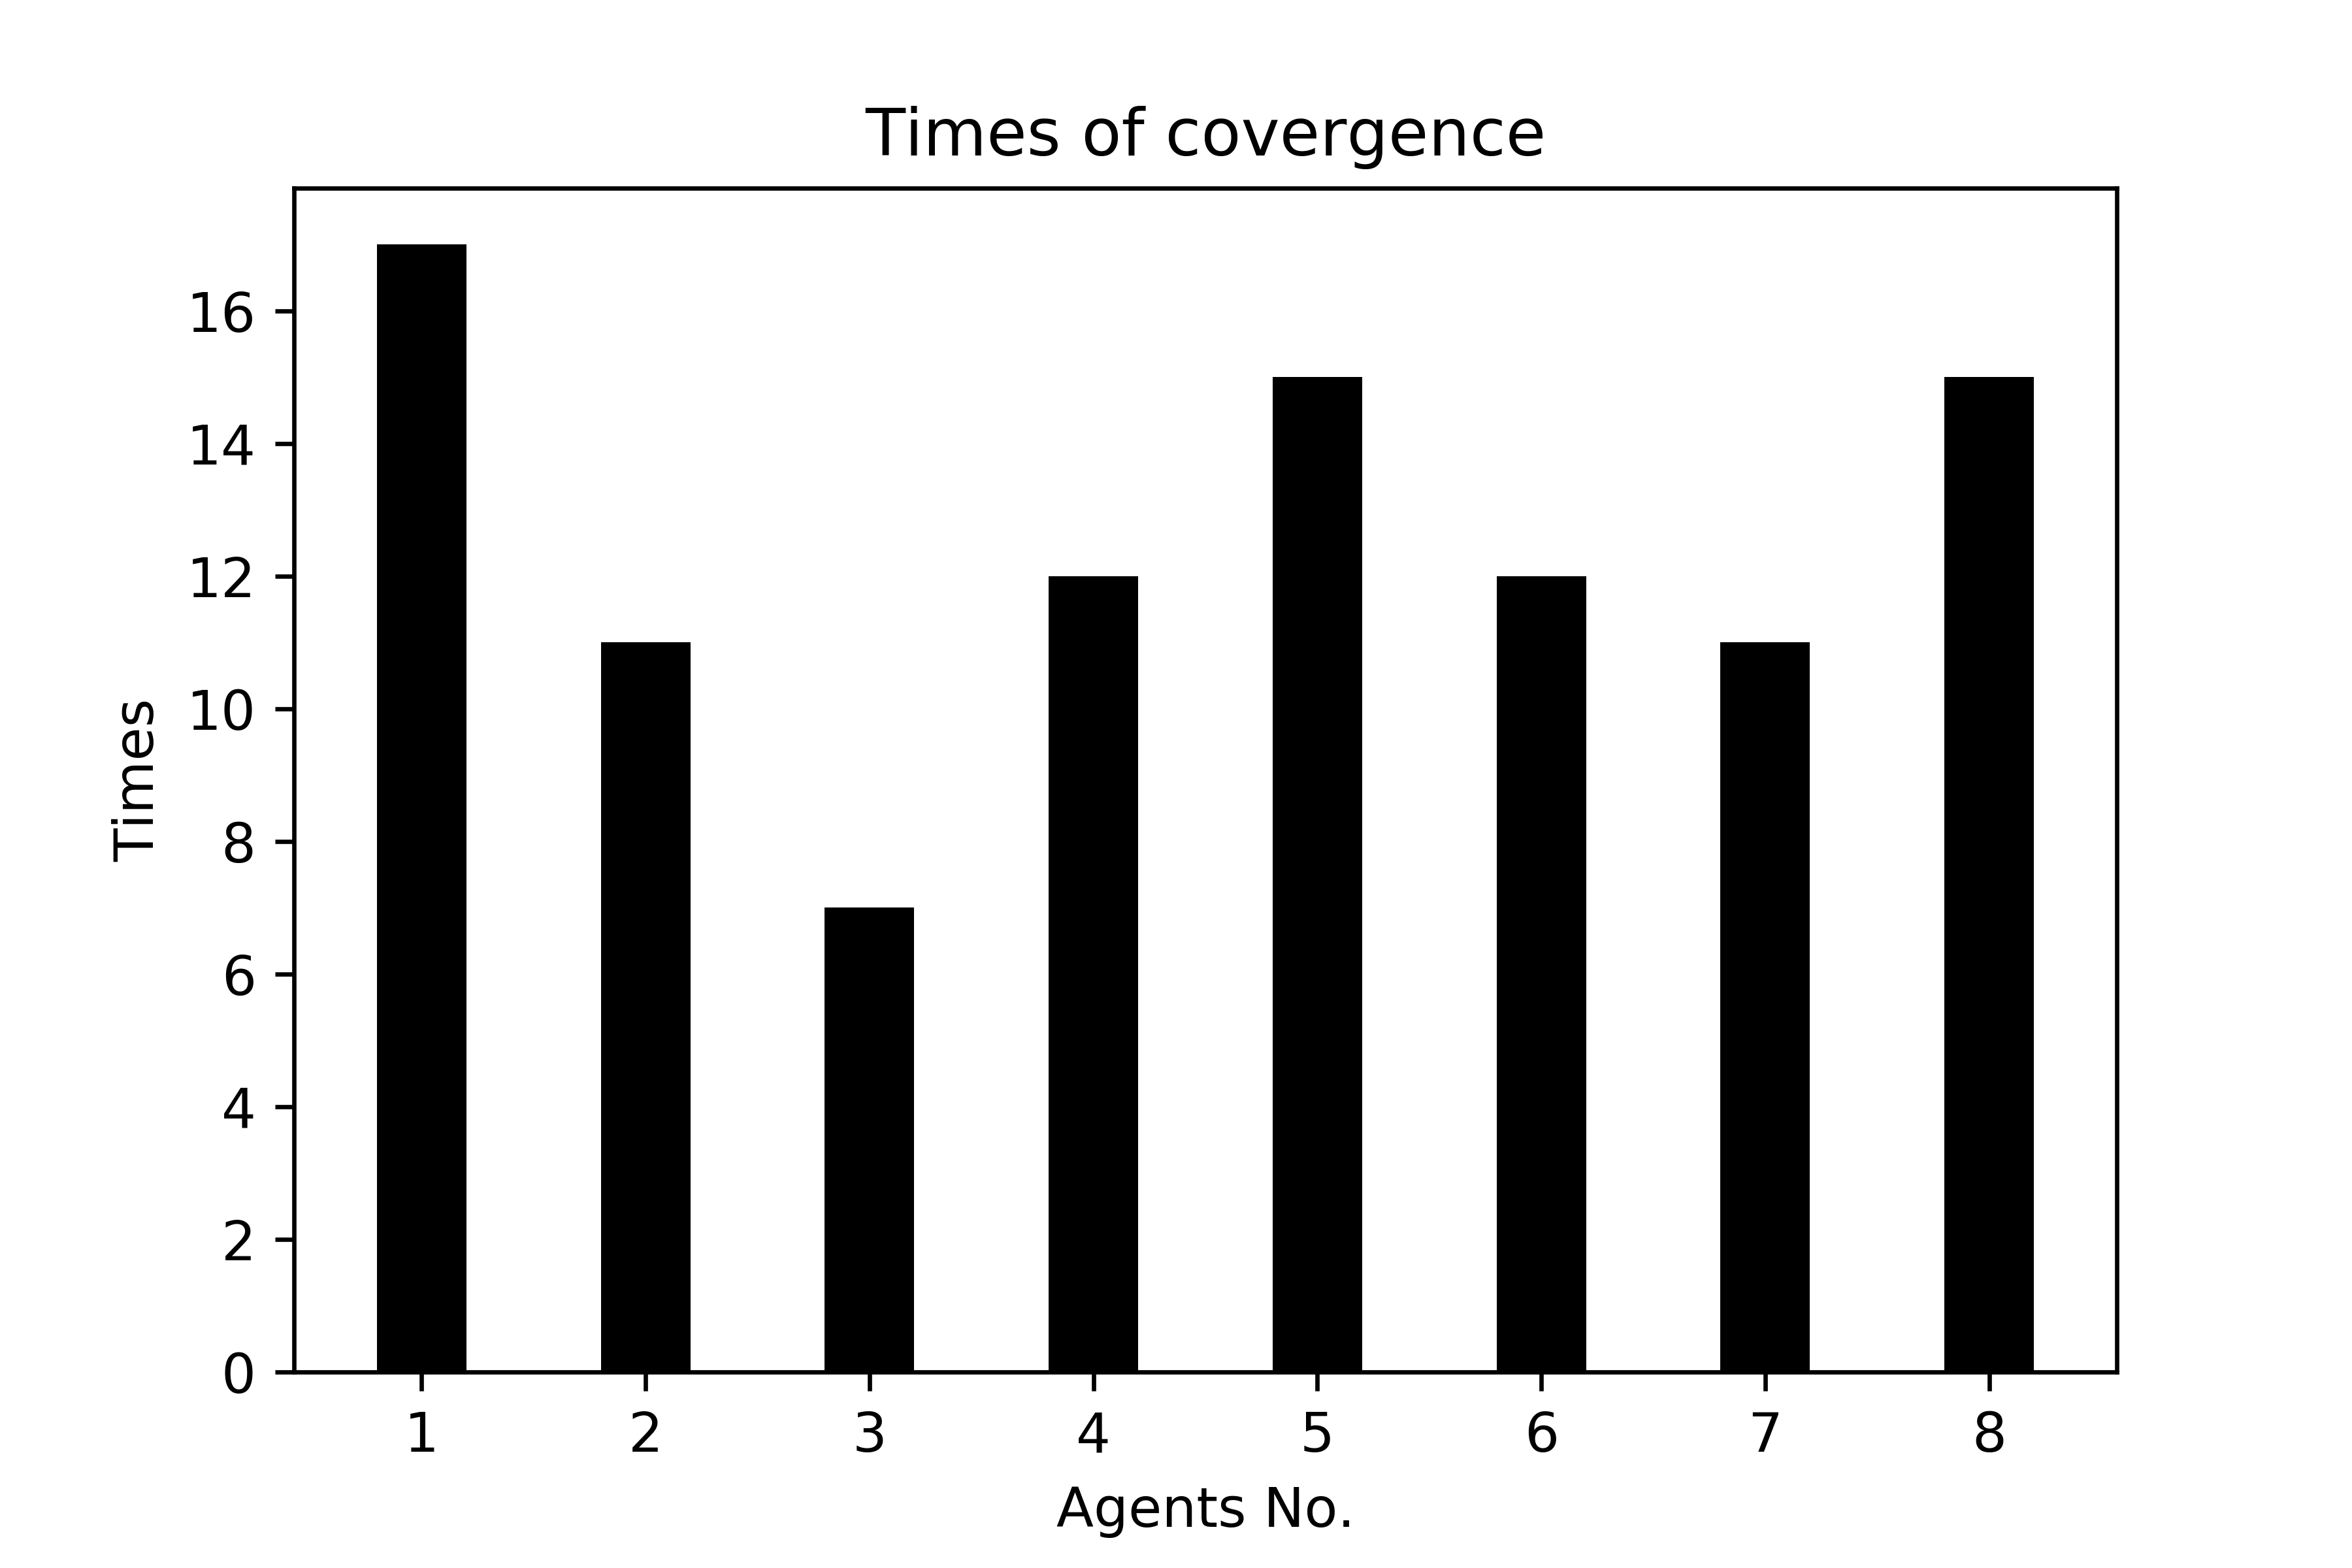
\includegraphics[width=0.9\textwidth]{agt50_3_800_100}
		\caption{Where the iterations converge}\label{agt50_3_800_100}
	\end{figure}
%
	\begin{figure}[H]
		\centering
		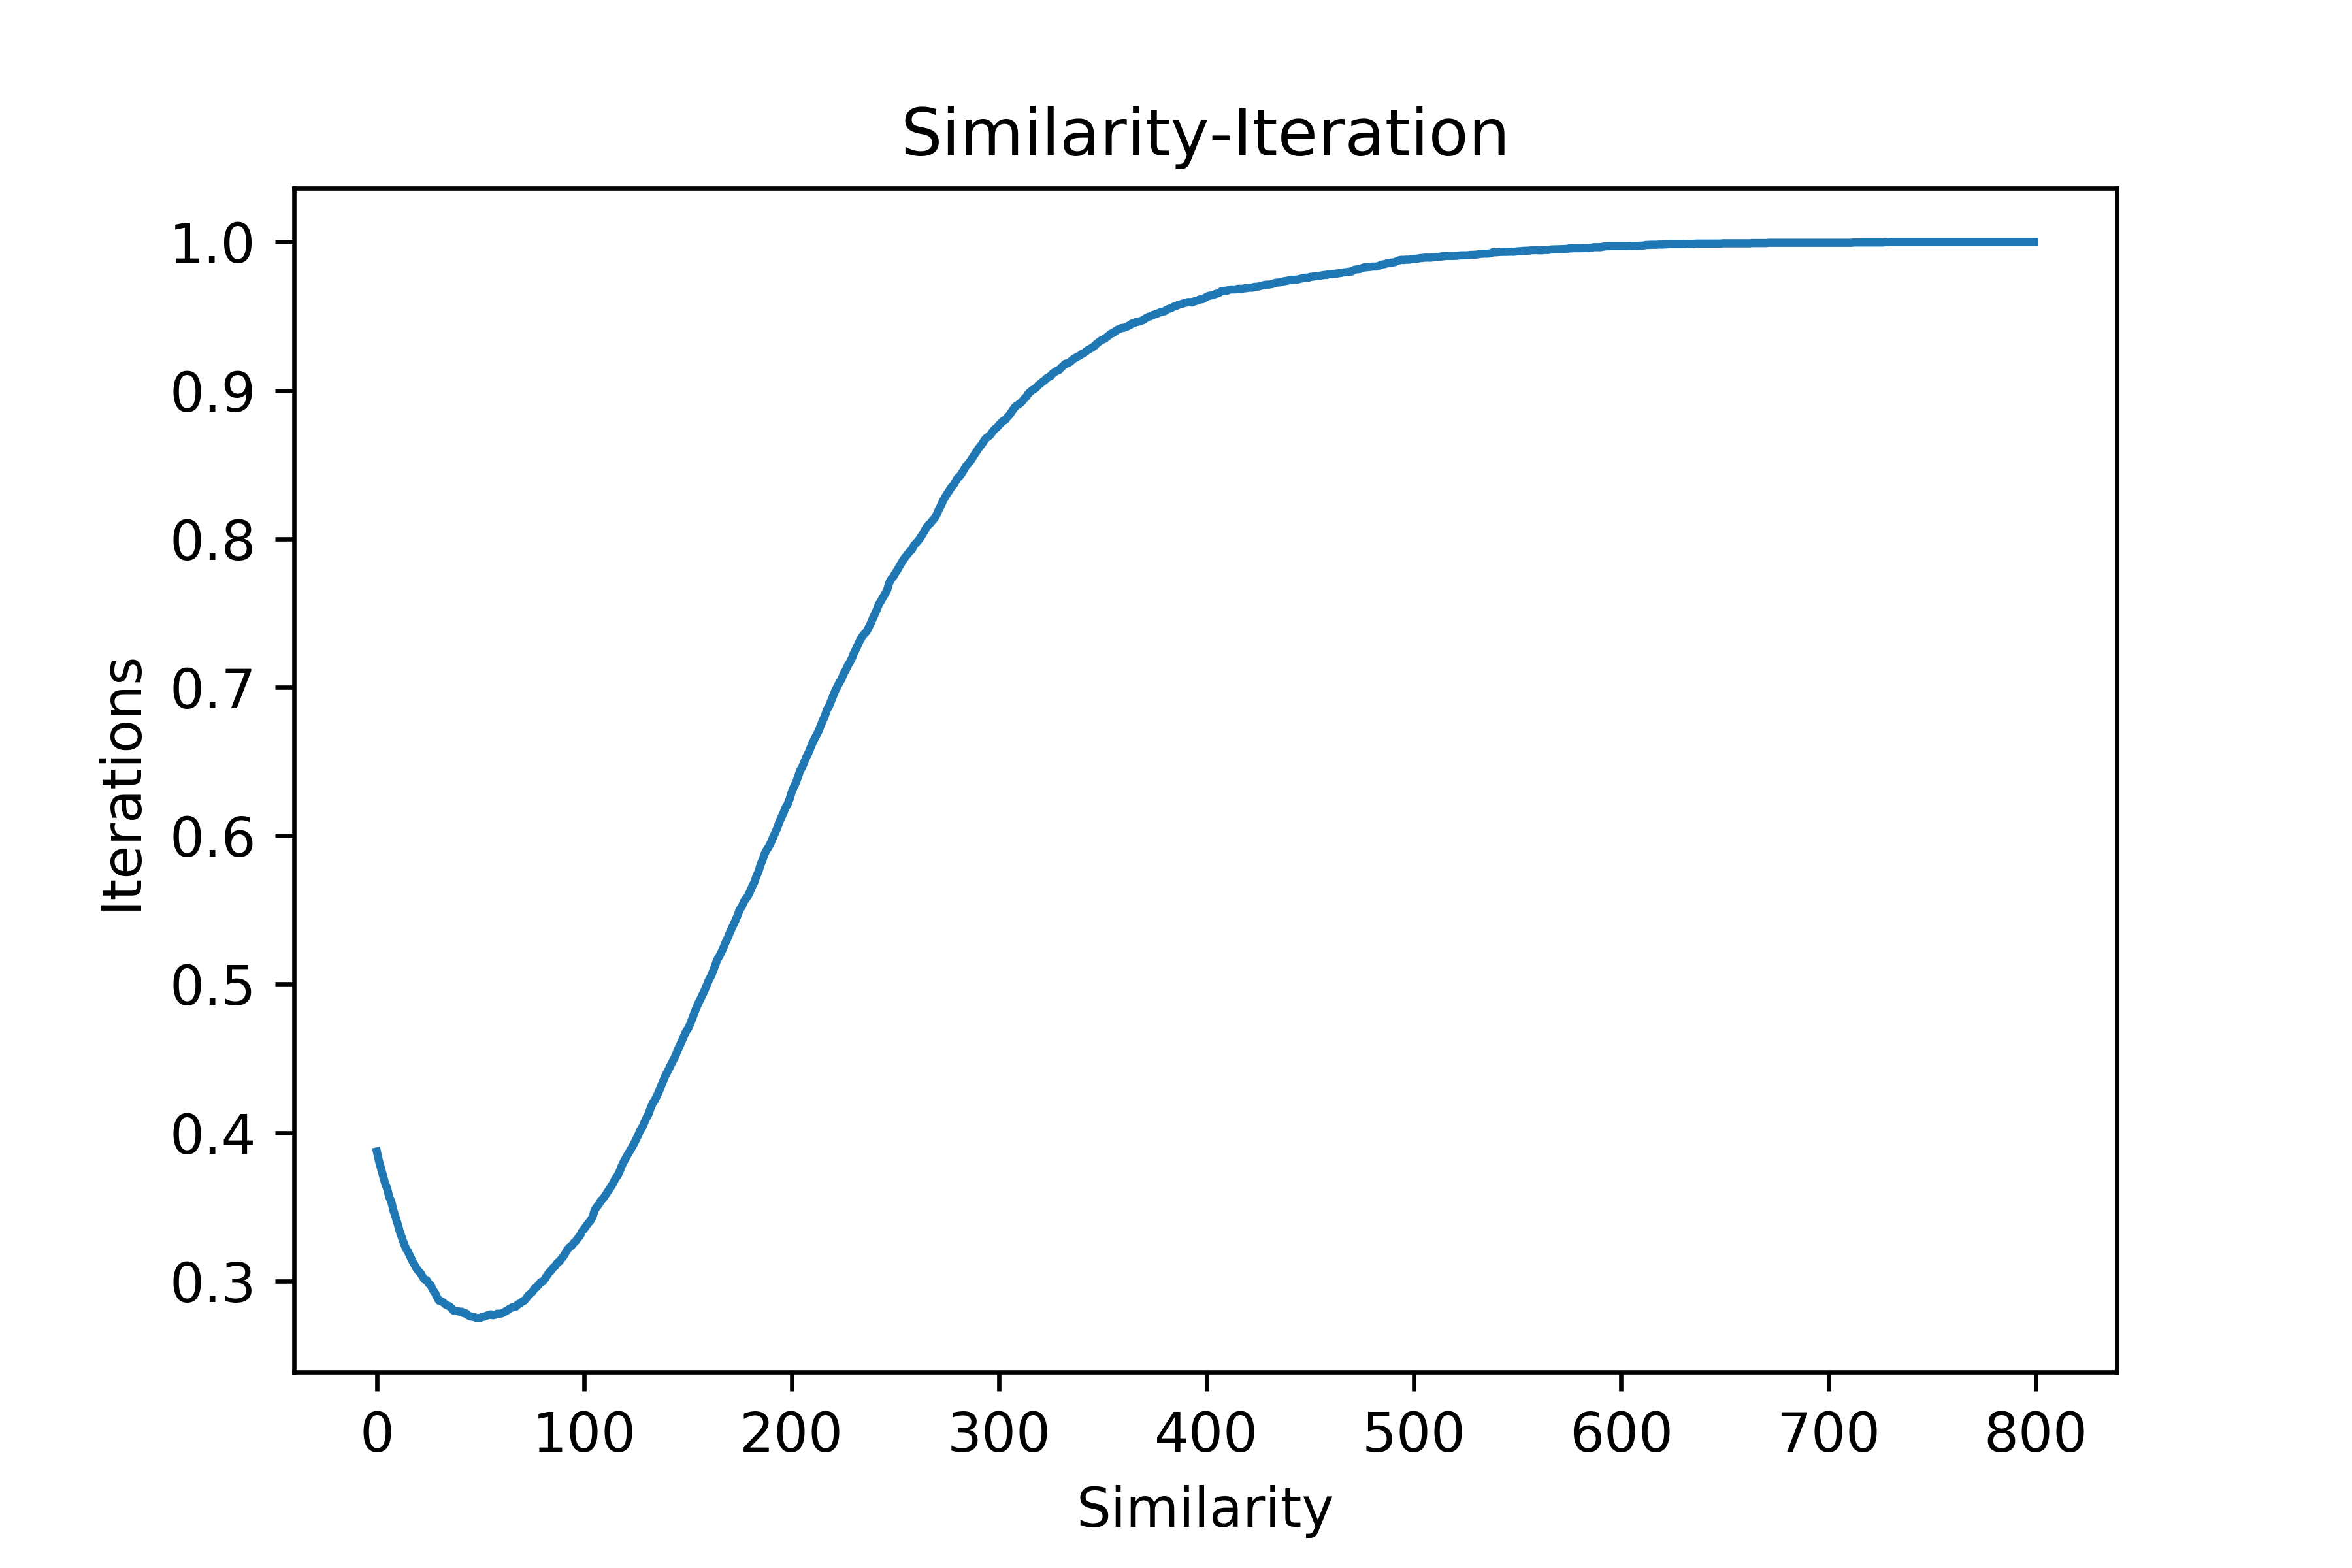
\includegraphics[width=0.9\textwidth]{Sim50_3_800_100}
		\caption{Similarity}\label{Sim50_3_800_100}
	\end{figure}
%
	\begin{figure}[H]
	\centering
	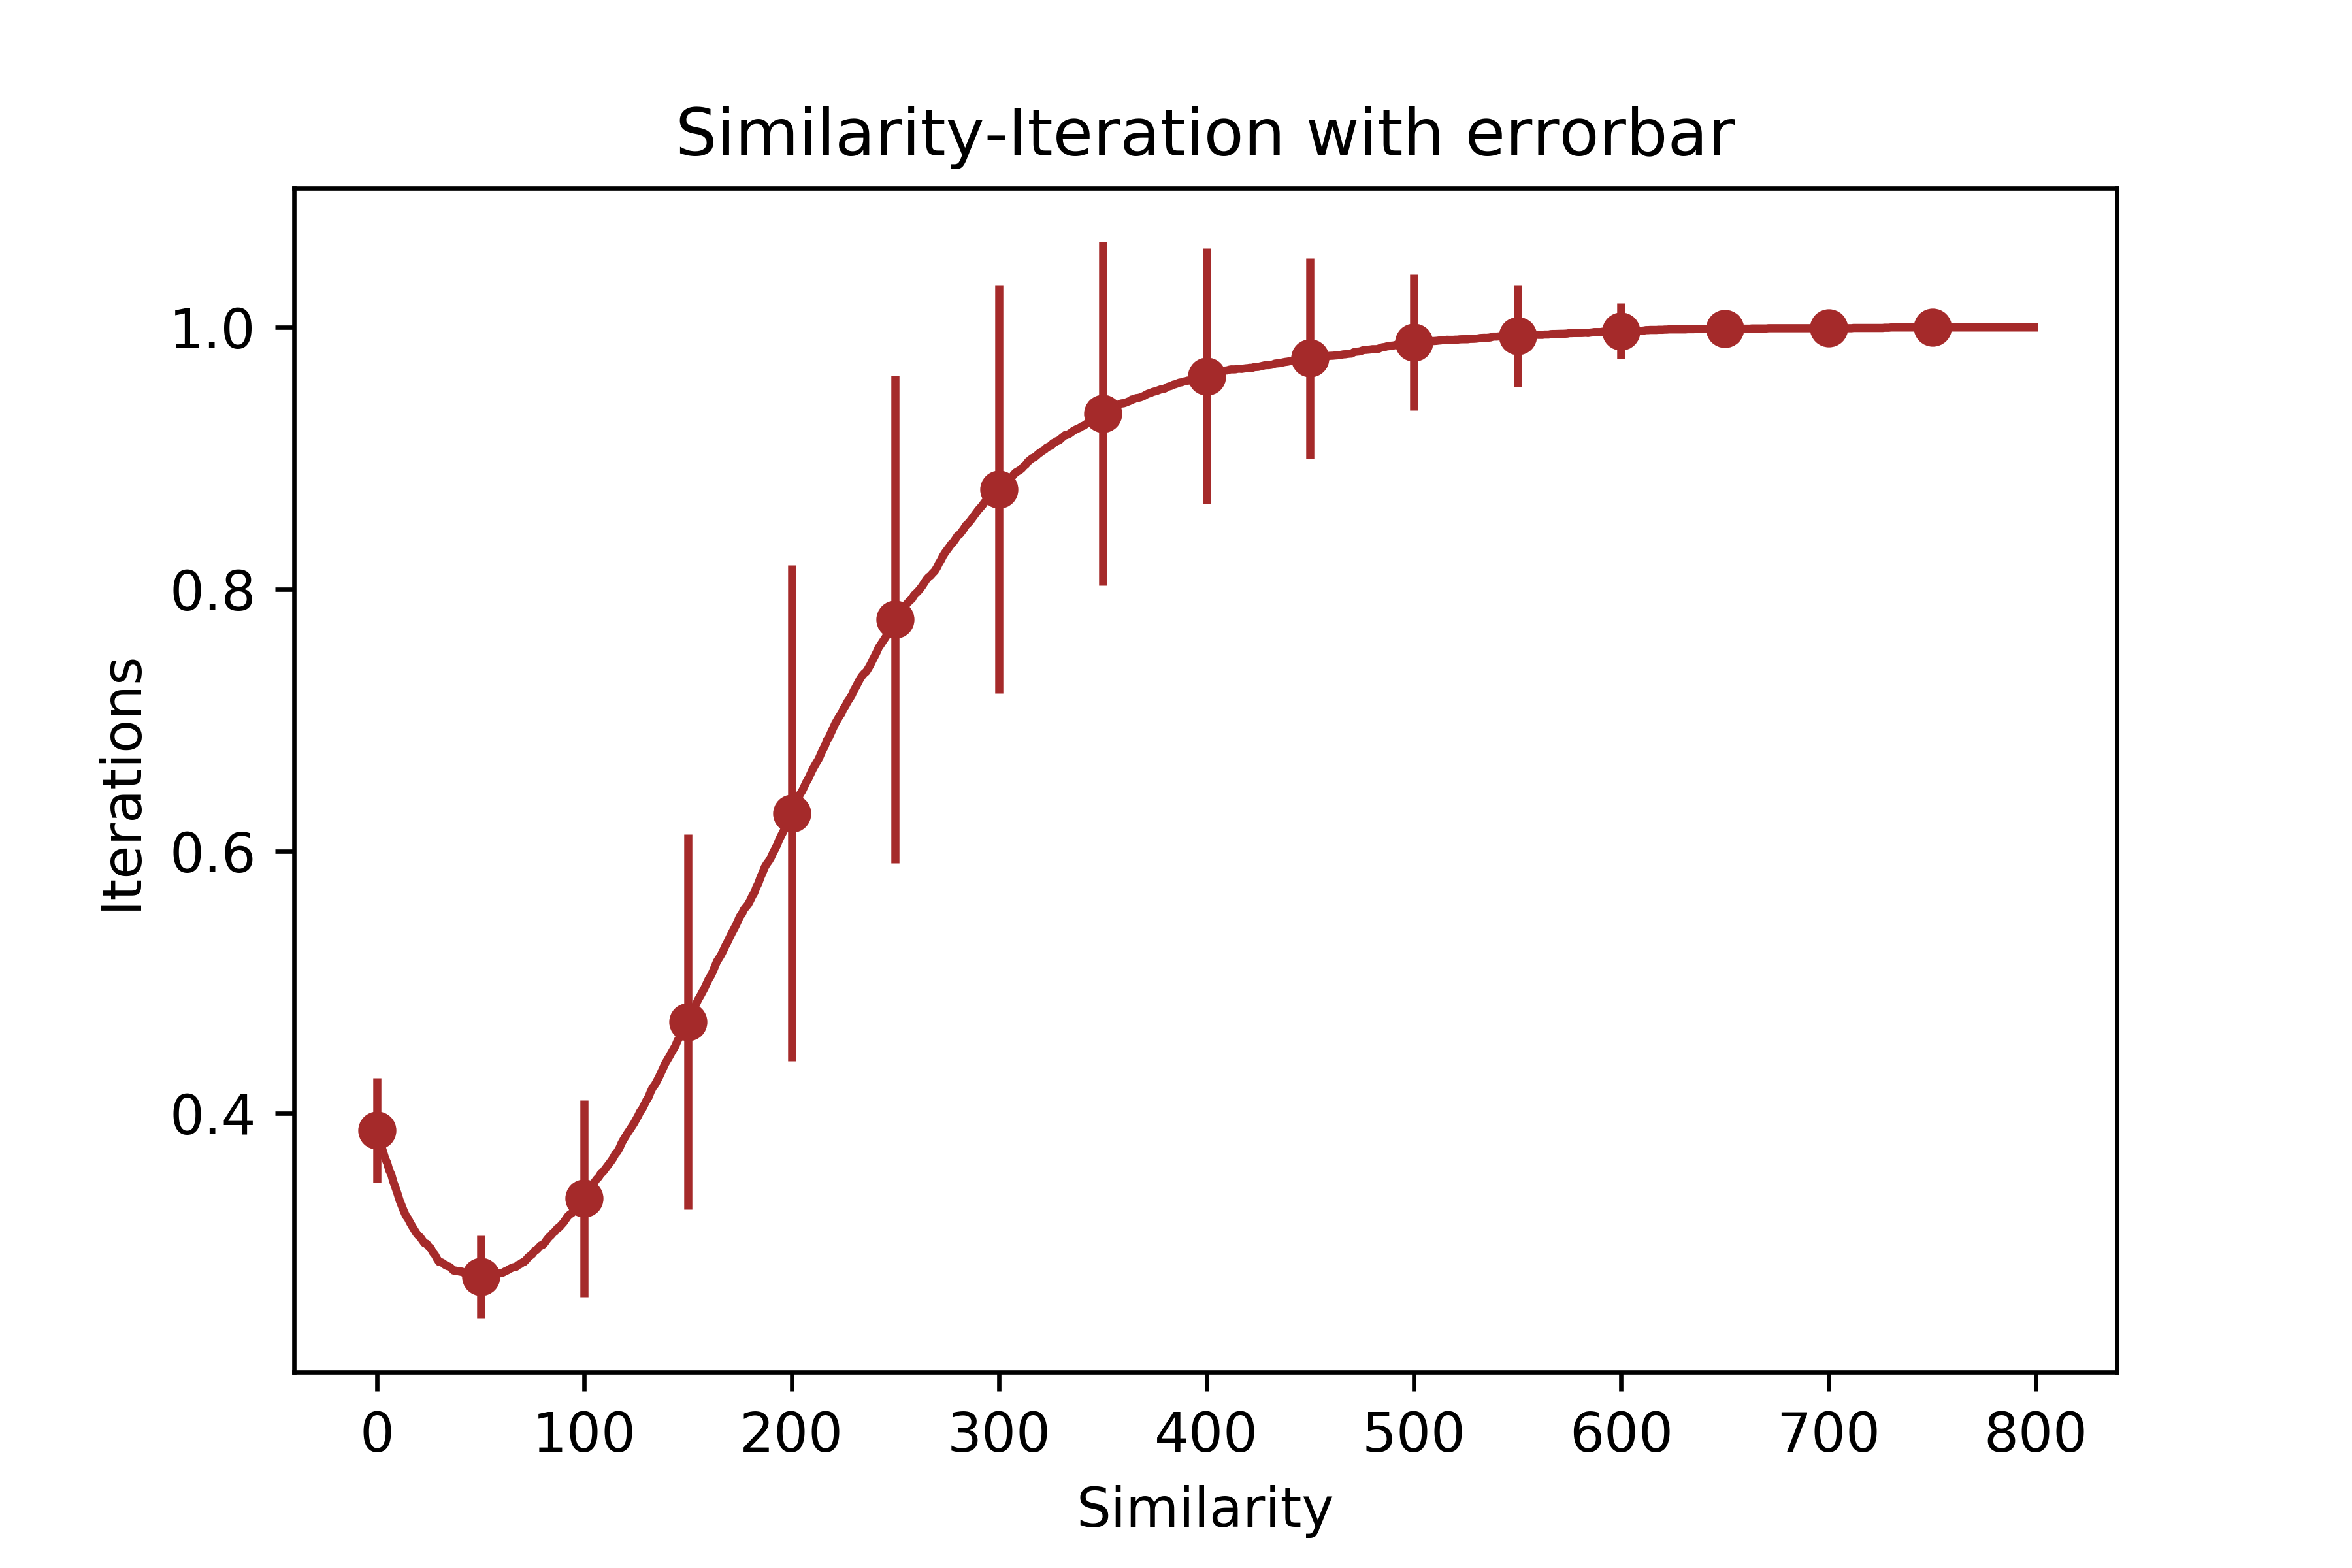
\includegraphics[width=0.9\textwidth]{SimErr50_3_800_100}
	\caption{Similarity with error bar}\label{SimErr50_3_800_100}
    \end{figure}
%
	\begin{figure}[H]
	\centering
	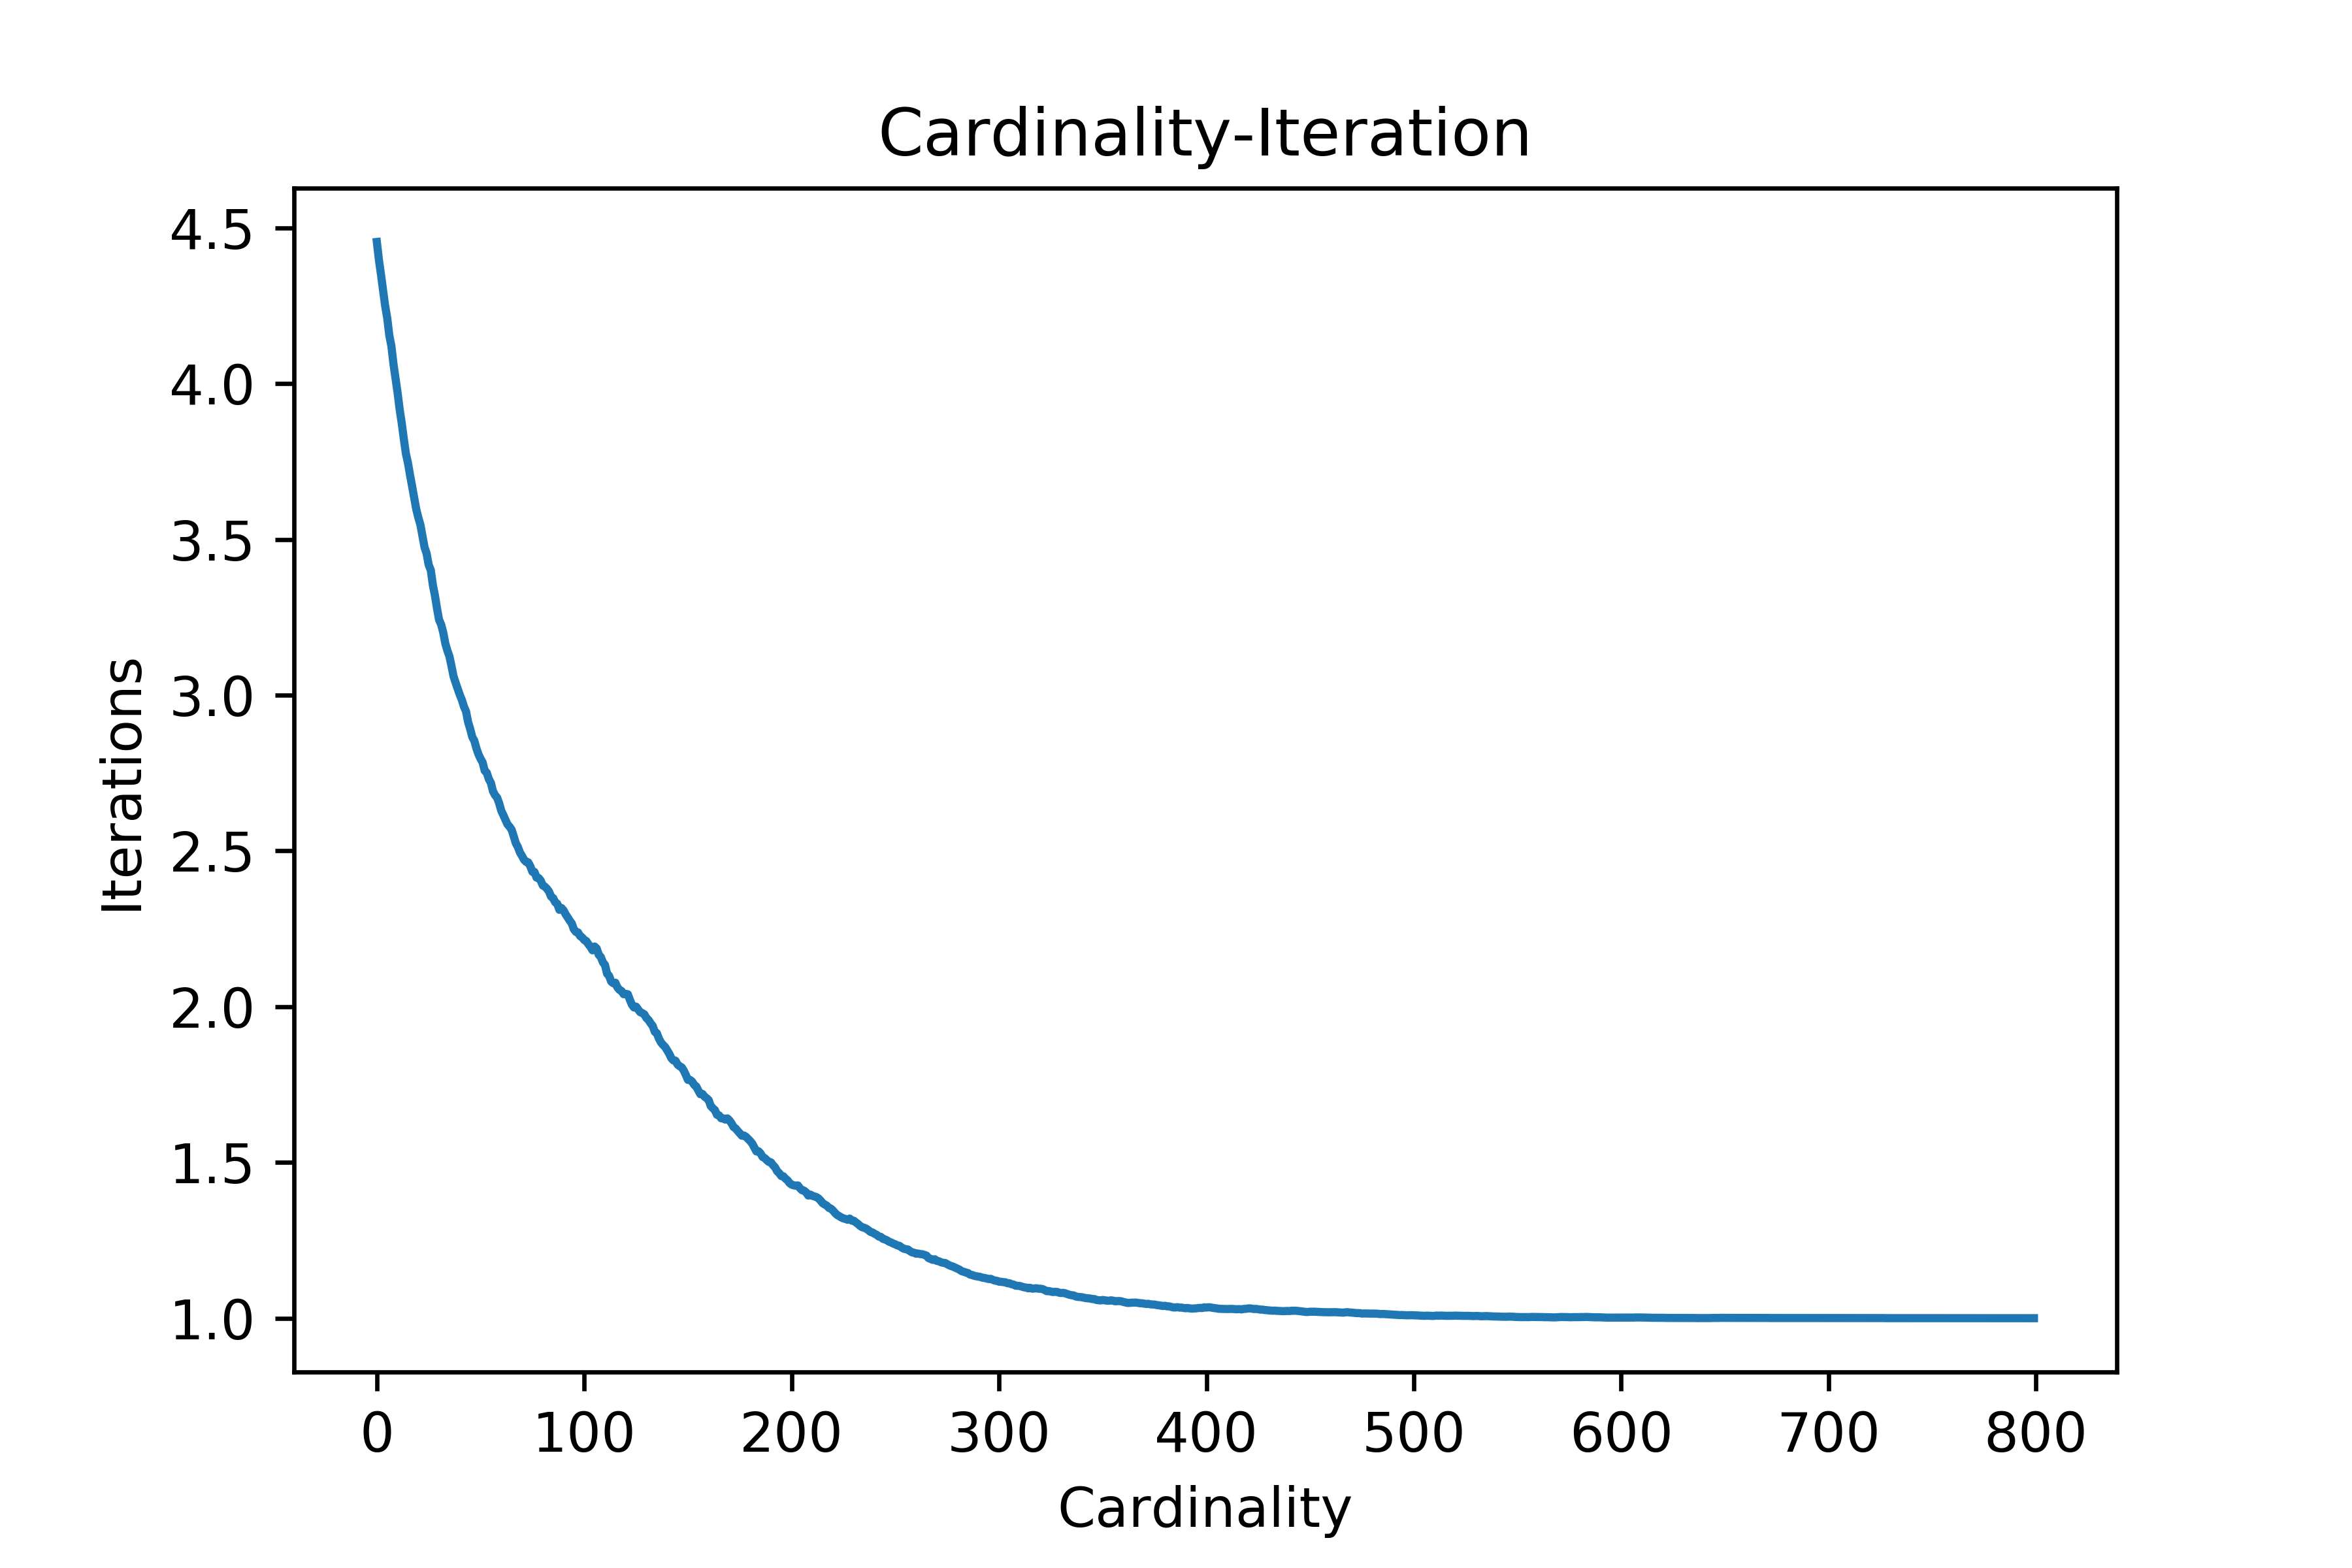
\includegraphics[width=0.9\textwidth]{Card50_3_800_100}
	\caption{Cardinality}\label{Card50_3_800_100}
   \end{figure}
%
	\begin{figure}[H]
	\centering
	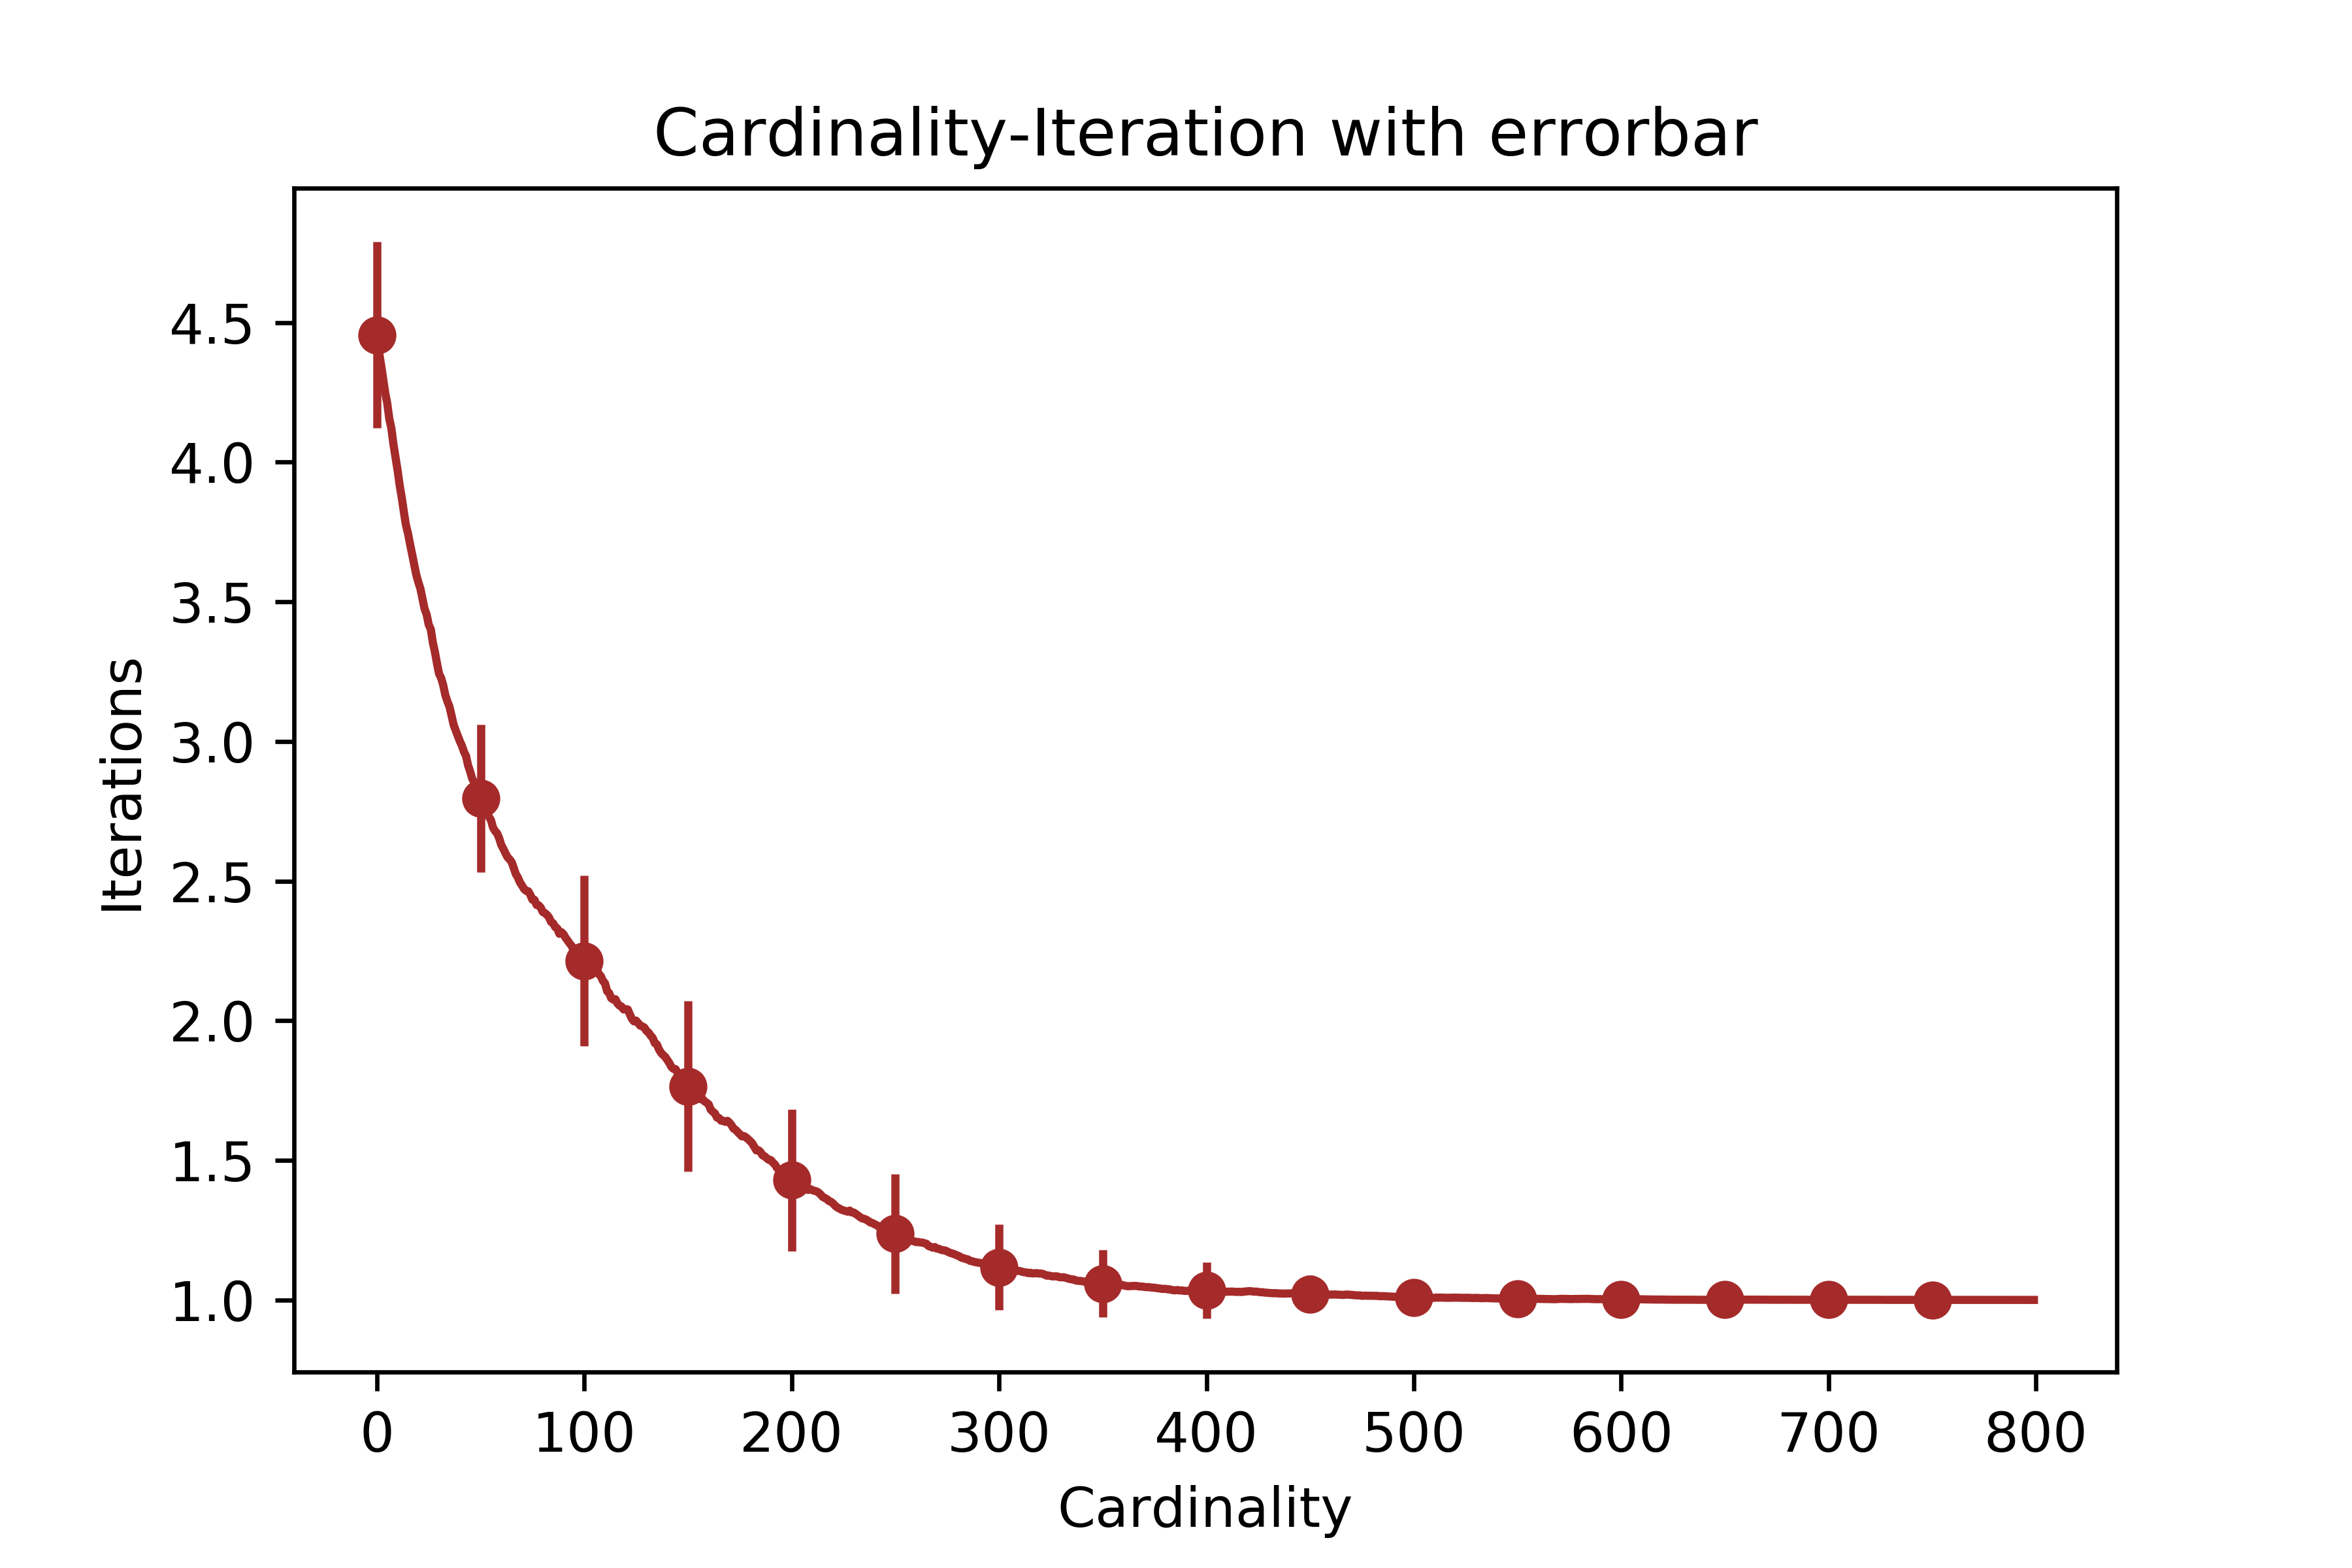
\includegraphics[width=0.9\textwidth]{CardErr50_3_800_100}
	\caption{Cardinality with error bar}\label{CardErr50_3_800_100}
    \end{figure}	

	\subsection{50\_4\_1000\_100}
	Time used: 87.256231800553$s$
	\begin{figure}[H]
		\centering
		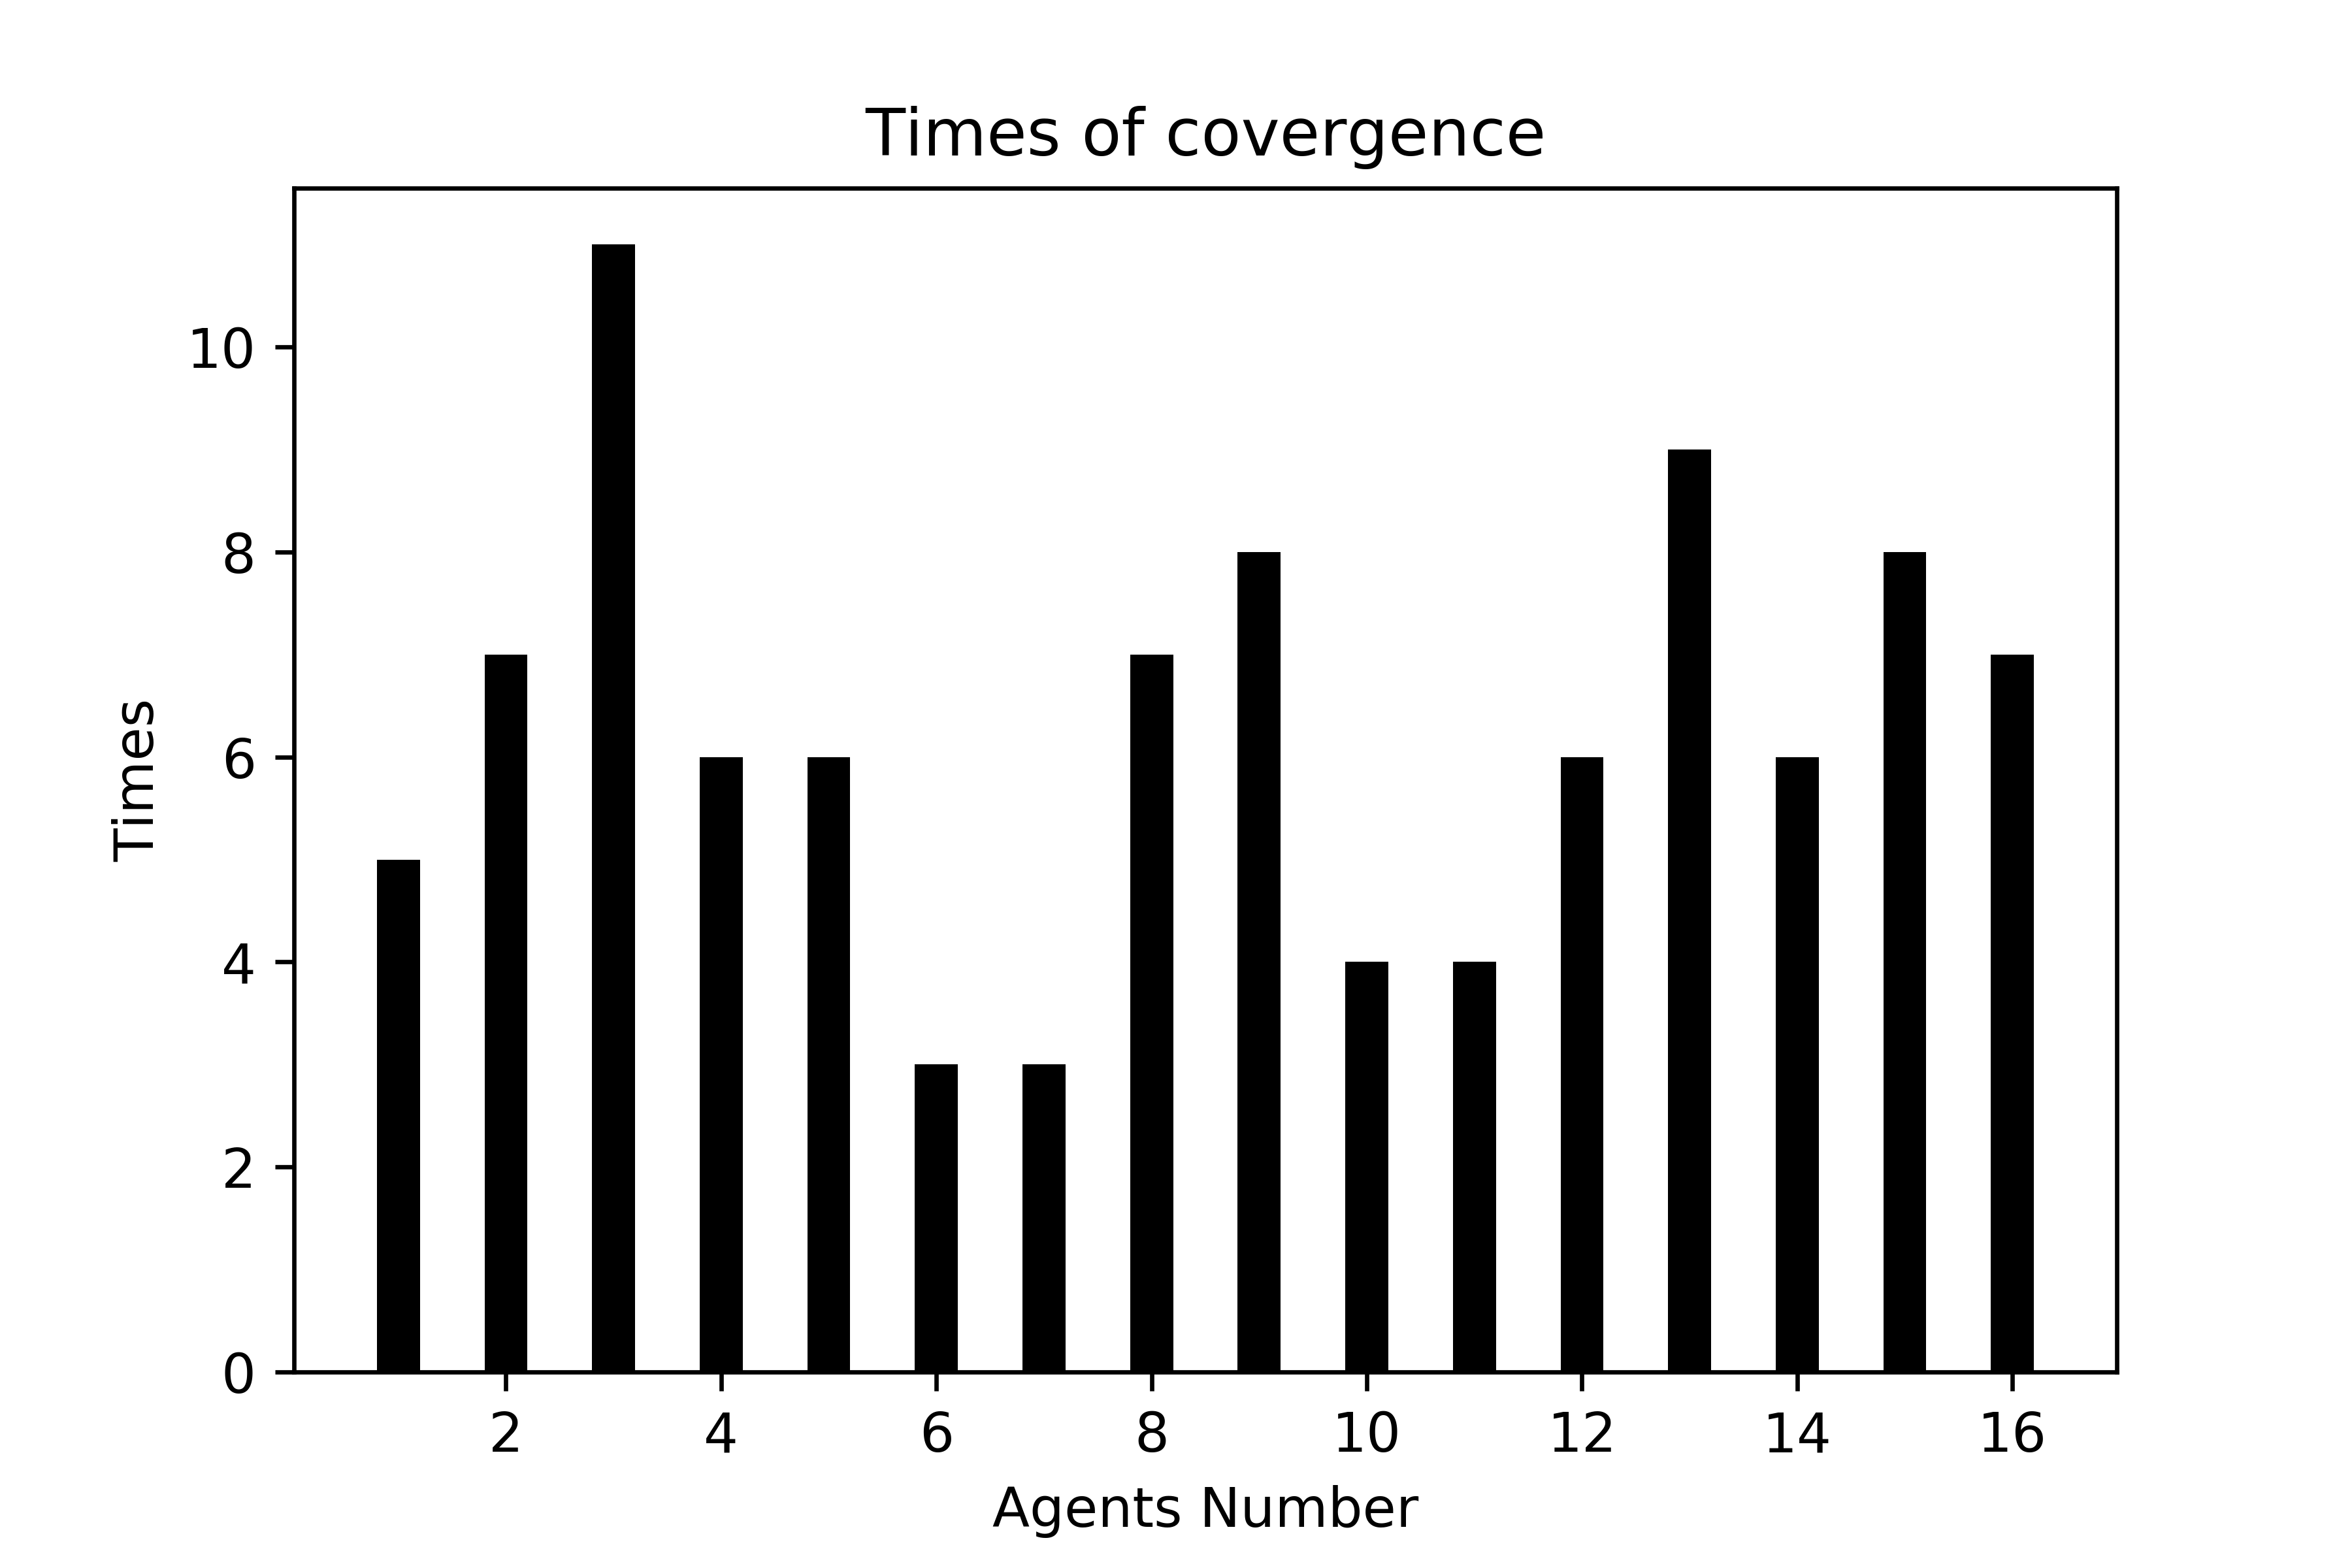
\includegraphics[width=0.9\textwidth]{agt50_4_1000_100}
		\caption{Where the iterations converge}\label{agt50_4_1000_100}
	\end{figure}
	%
	\begin{figure}[H]
		\centering
		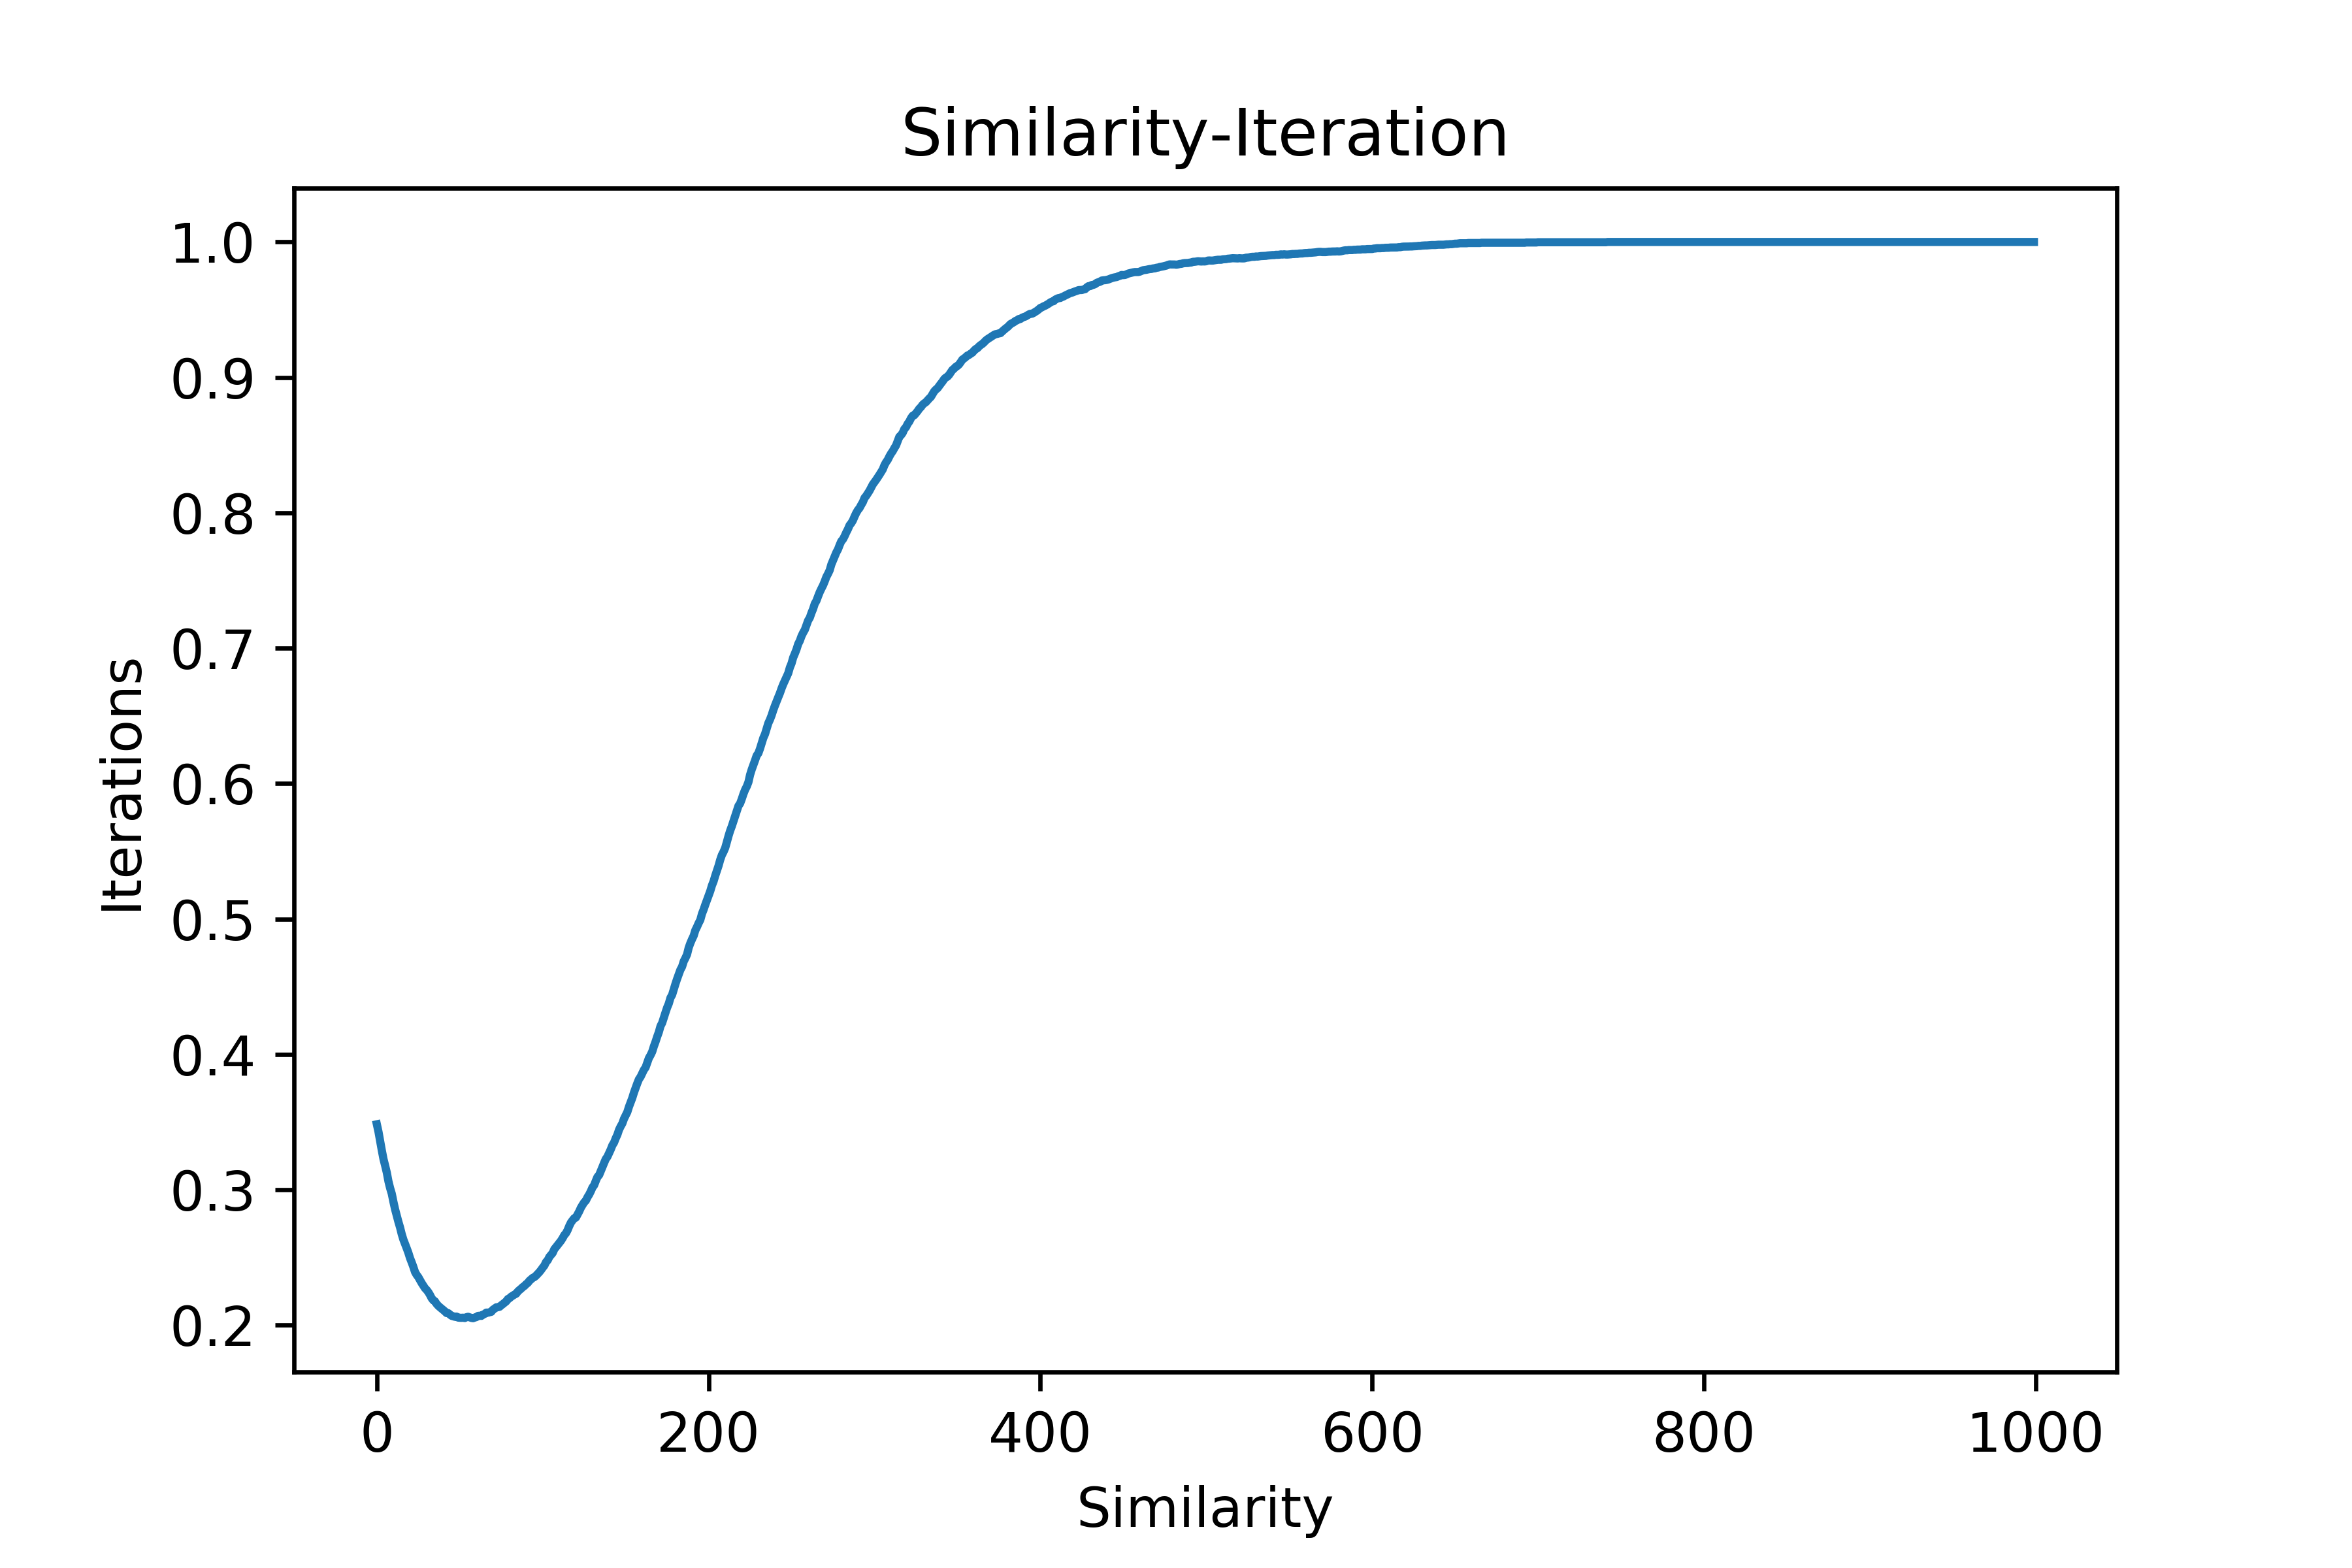
\includegraphics[width=0.9\textwidth]{Sim50_4_1000_100}
		\caption{Similarity}\label{Sim50_4_1000_100}
	\end{figure}
	%
	\begin{figure}[H]
		\centering
		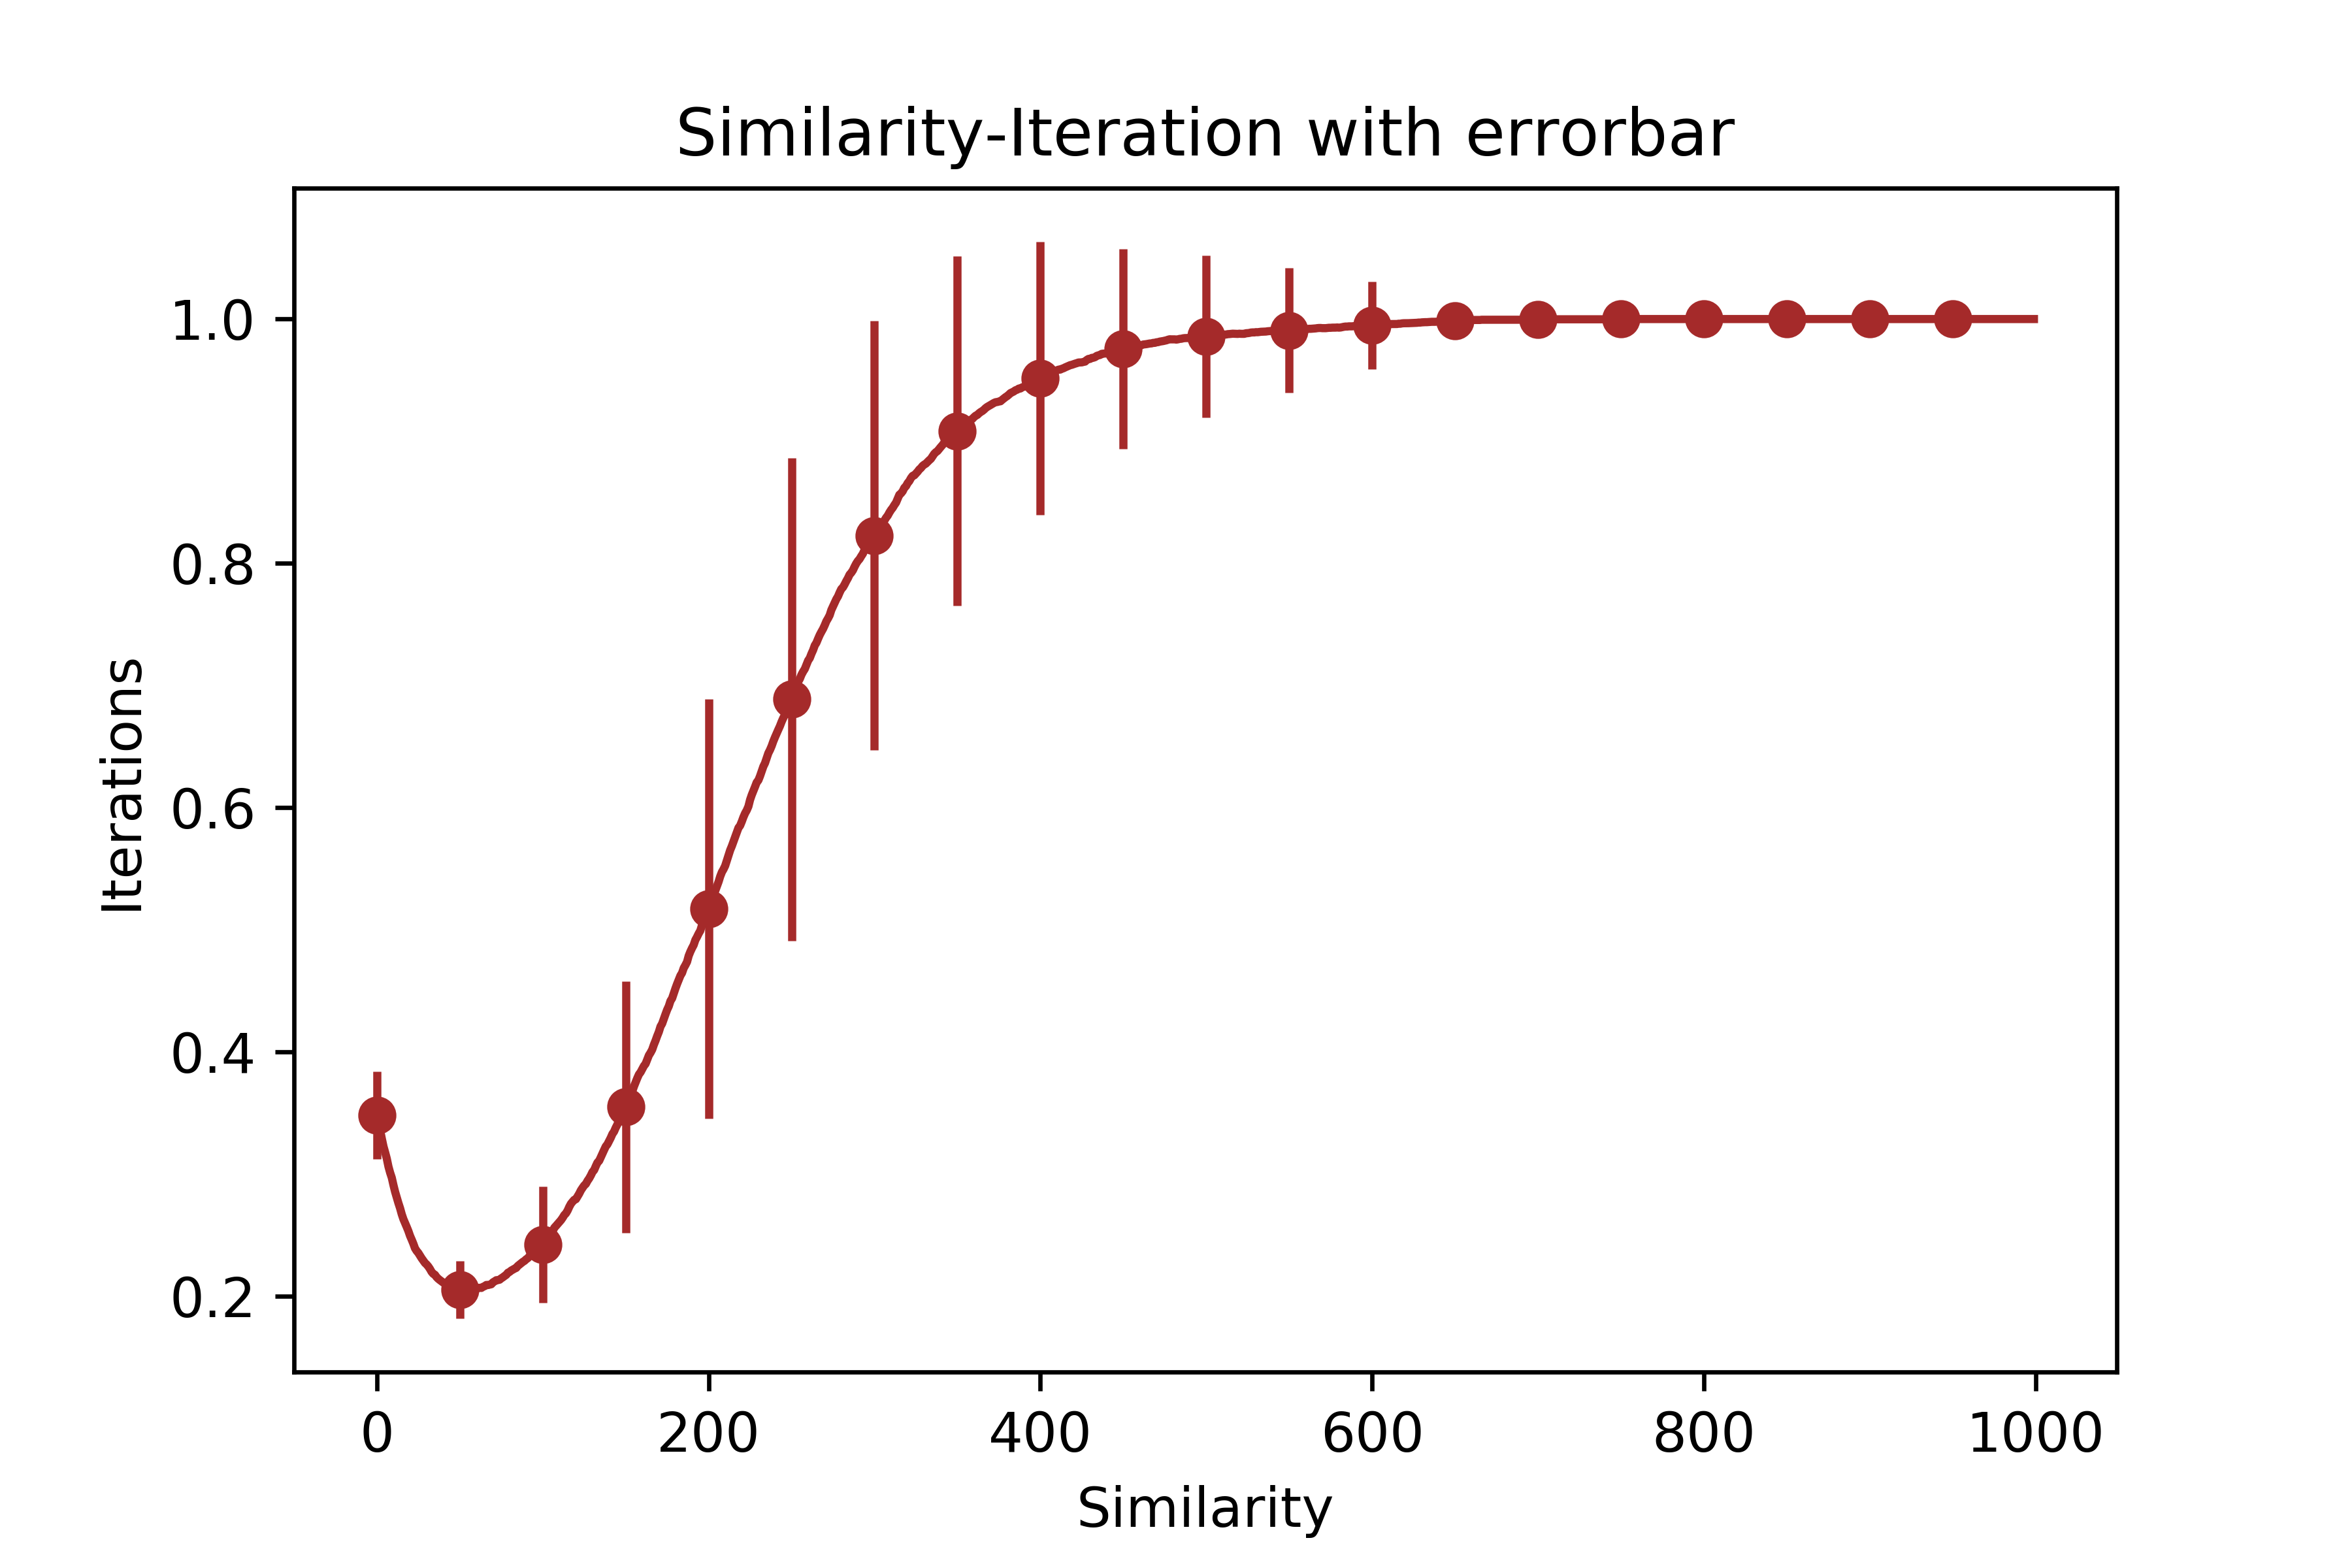
\includegraphics[width=0.9\textwidth]{SimErr50_4_1000_100}
		\caption{Similarity with error bar}\label{SimErr50_4_1000_100}
	\end{figure}
	%
	\begin{figure}[H]
		\centering
		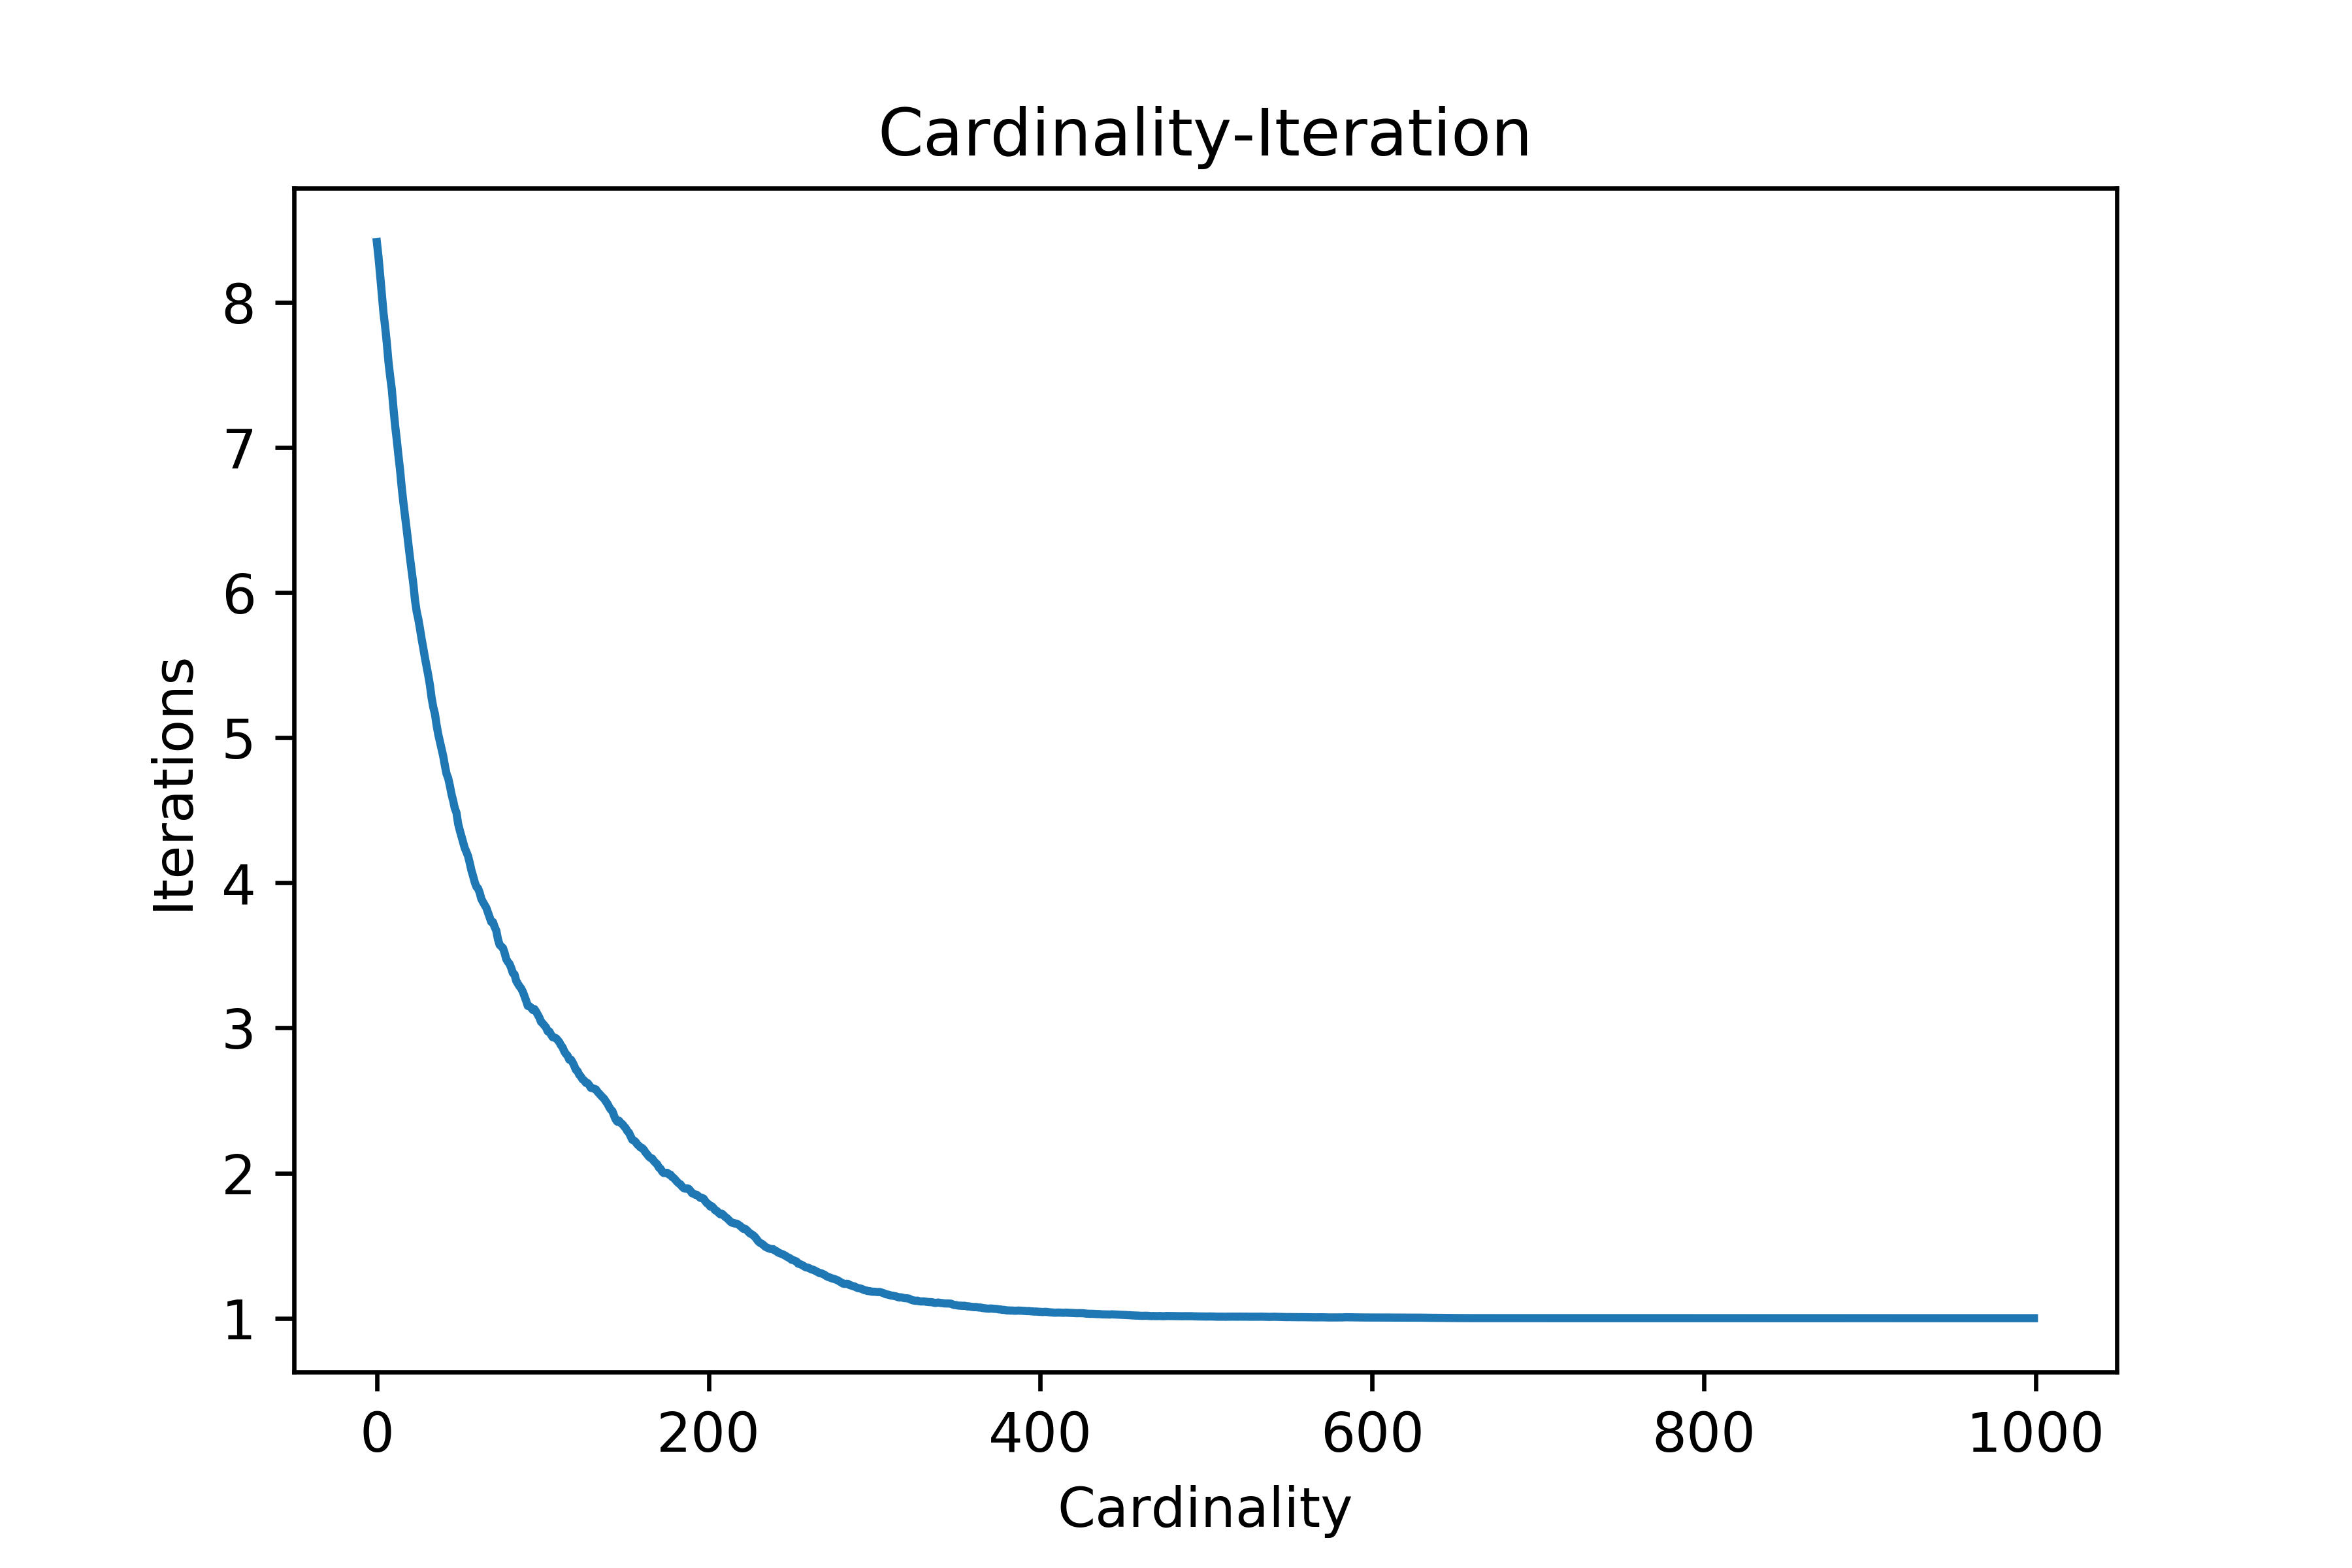
\includegraphics[width=0.9\textwidth]{Card50_4_1000_100}
		\caption{Cardinality}\label{Card50_4_1000_100}
	\end{figure}
	%
	\begin{figure}[H]
		\centering
		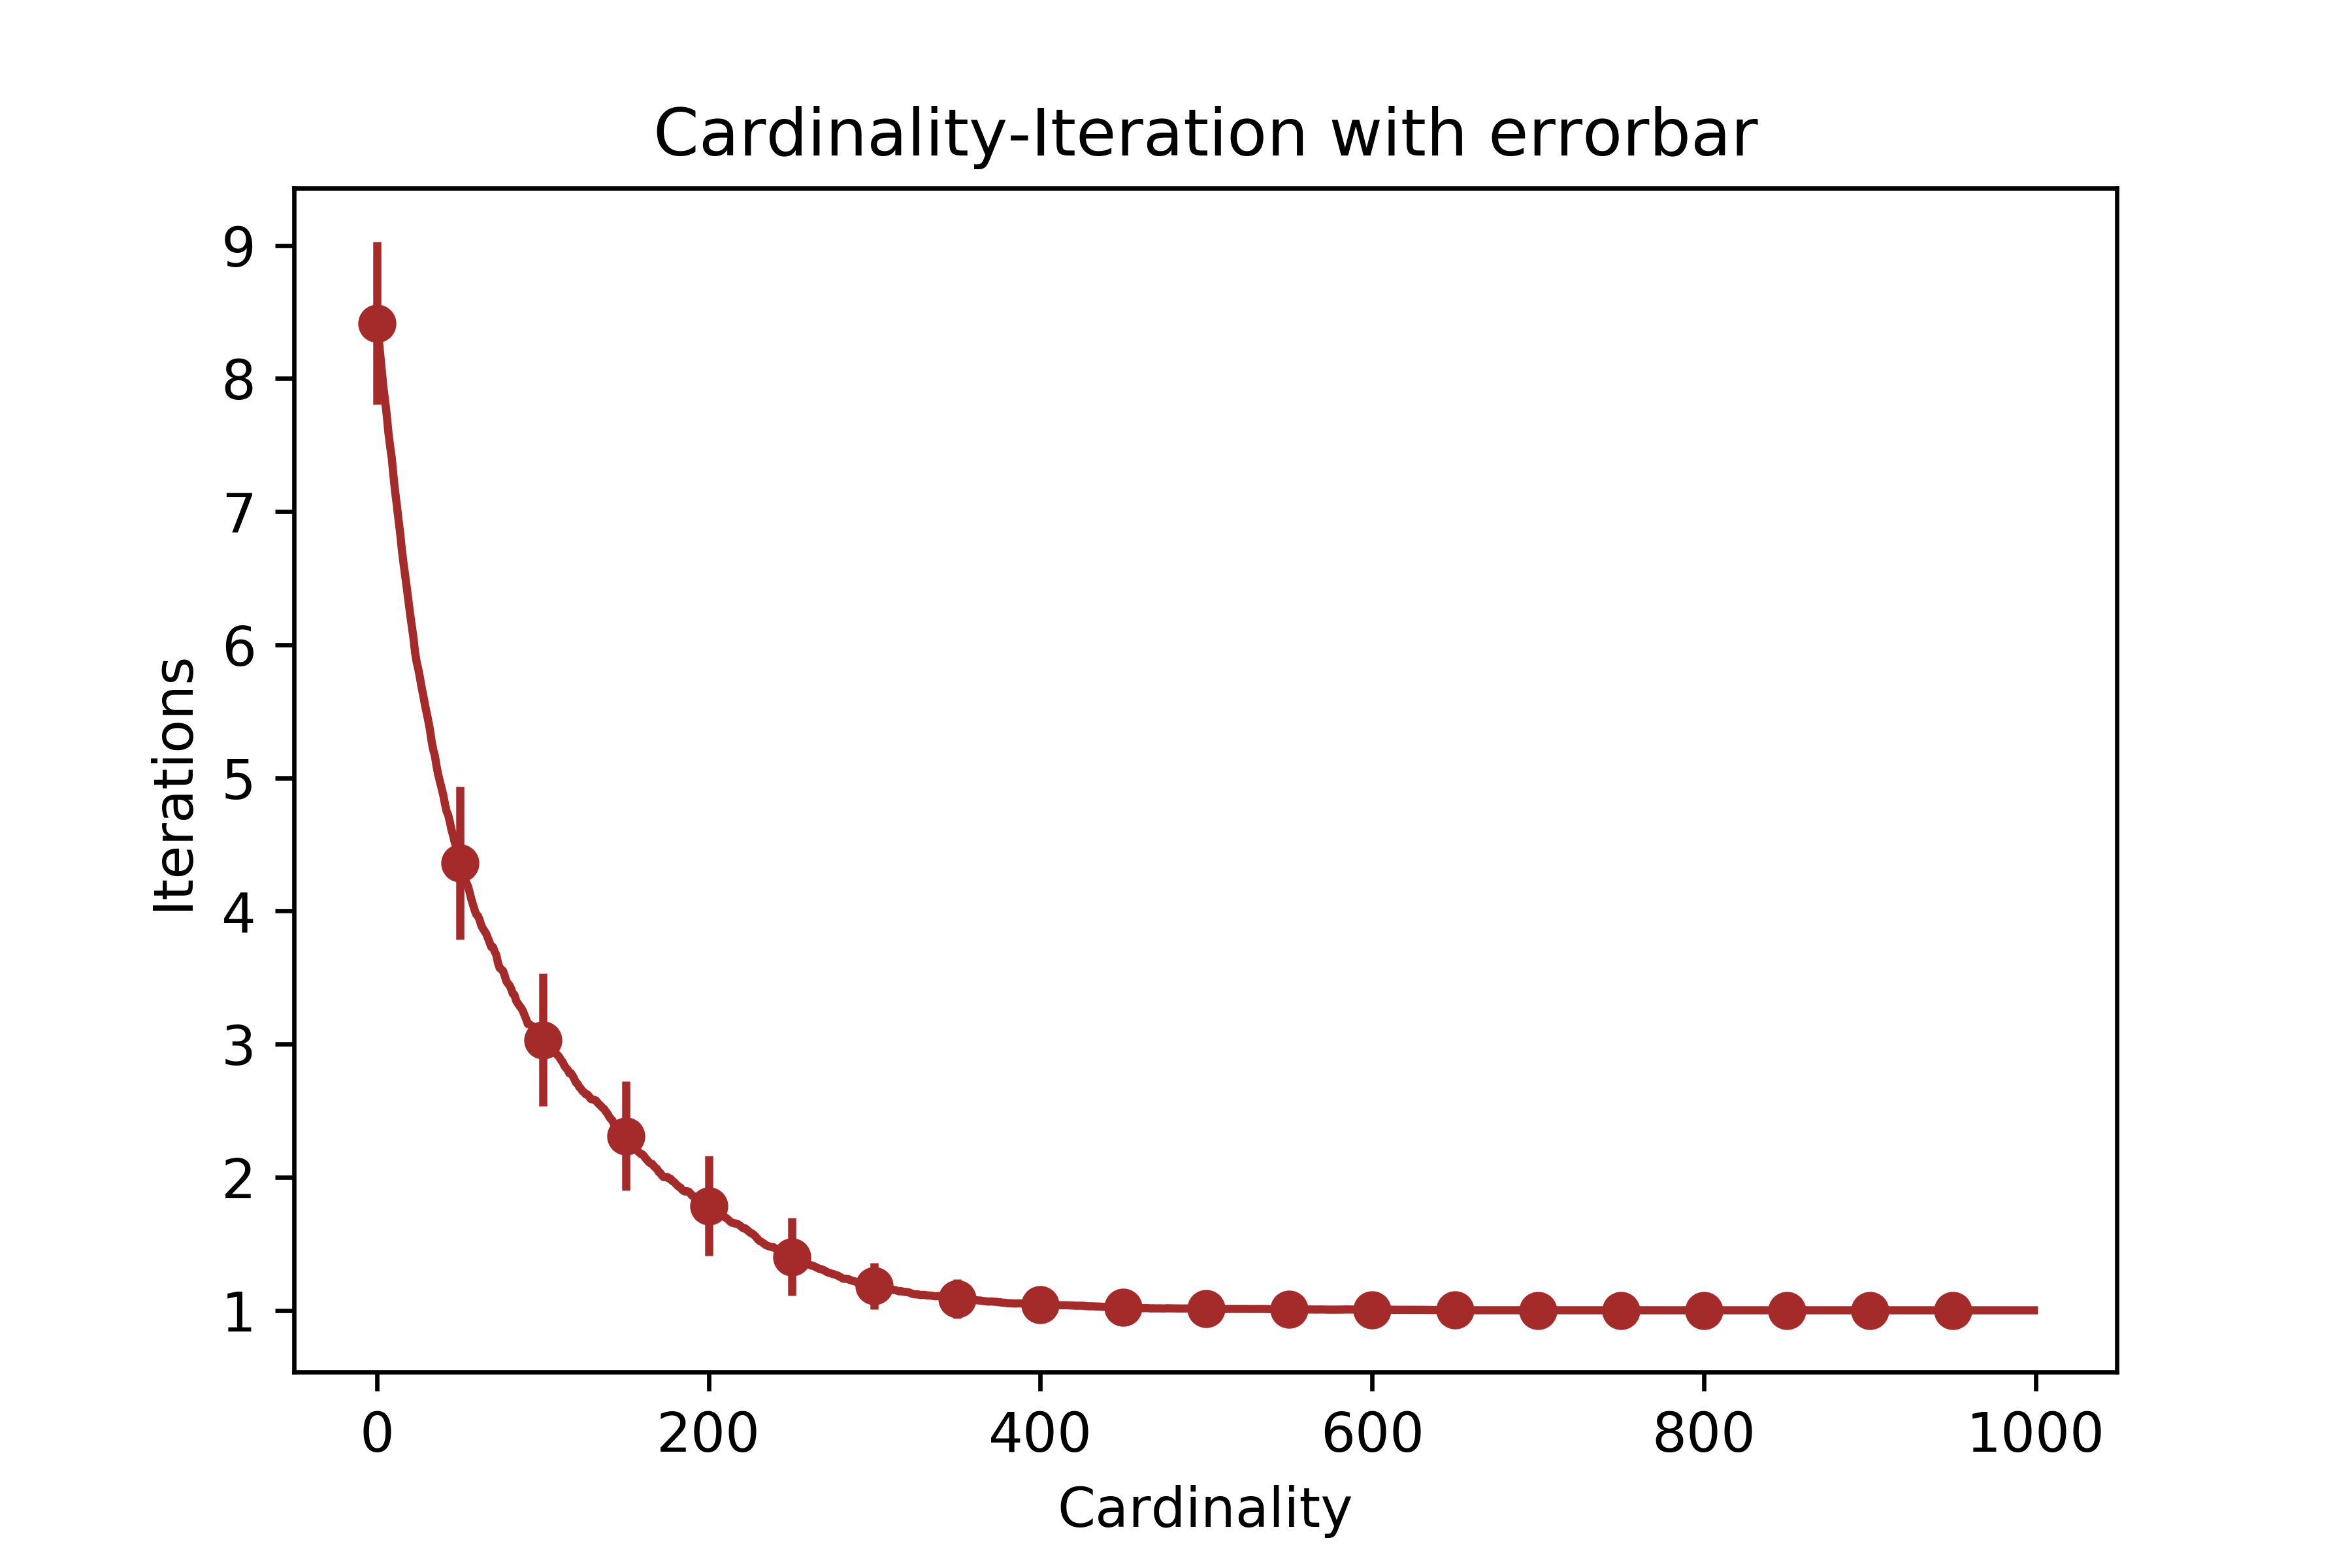
\includegraphics[width=0.9\textwidth]{CardErr50_4_1000_100}
		\caption{Cardinality with error bar}\label{CardErr50_4_1000_100}
	\end{figure}
    \subsection{50\_4\_1000\_300}
    Time used: 247.07707320986628		
    	\begin{figure}[H]
    	\centering
    	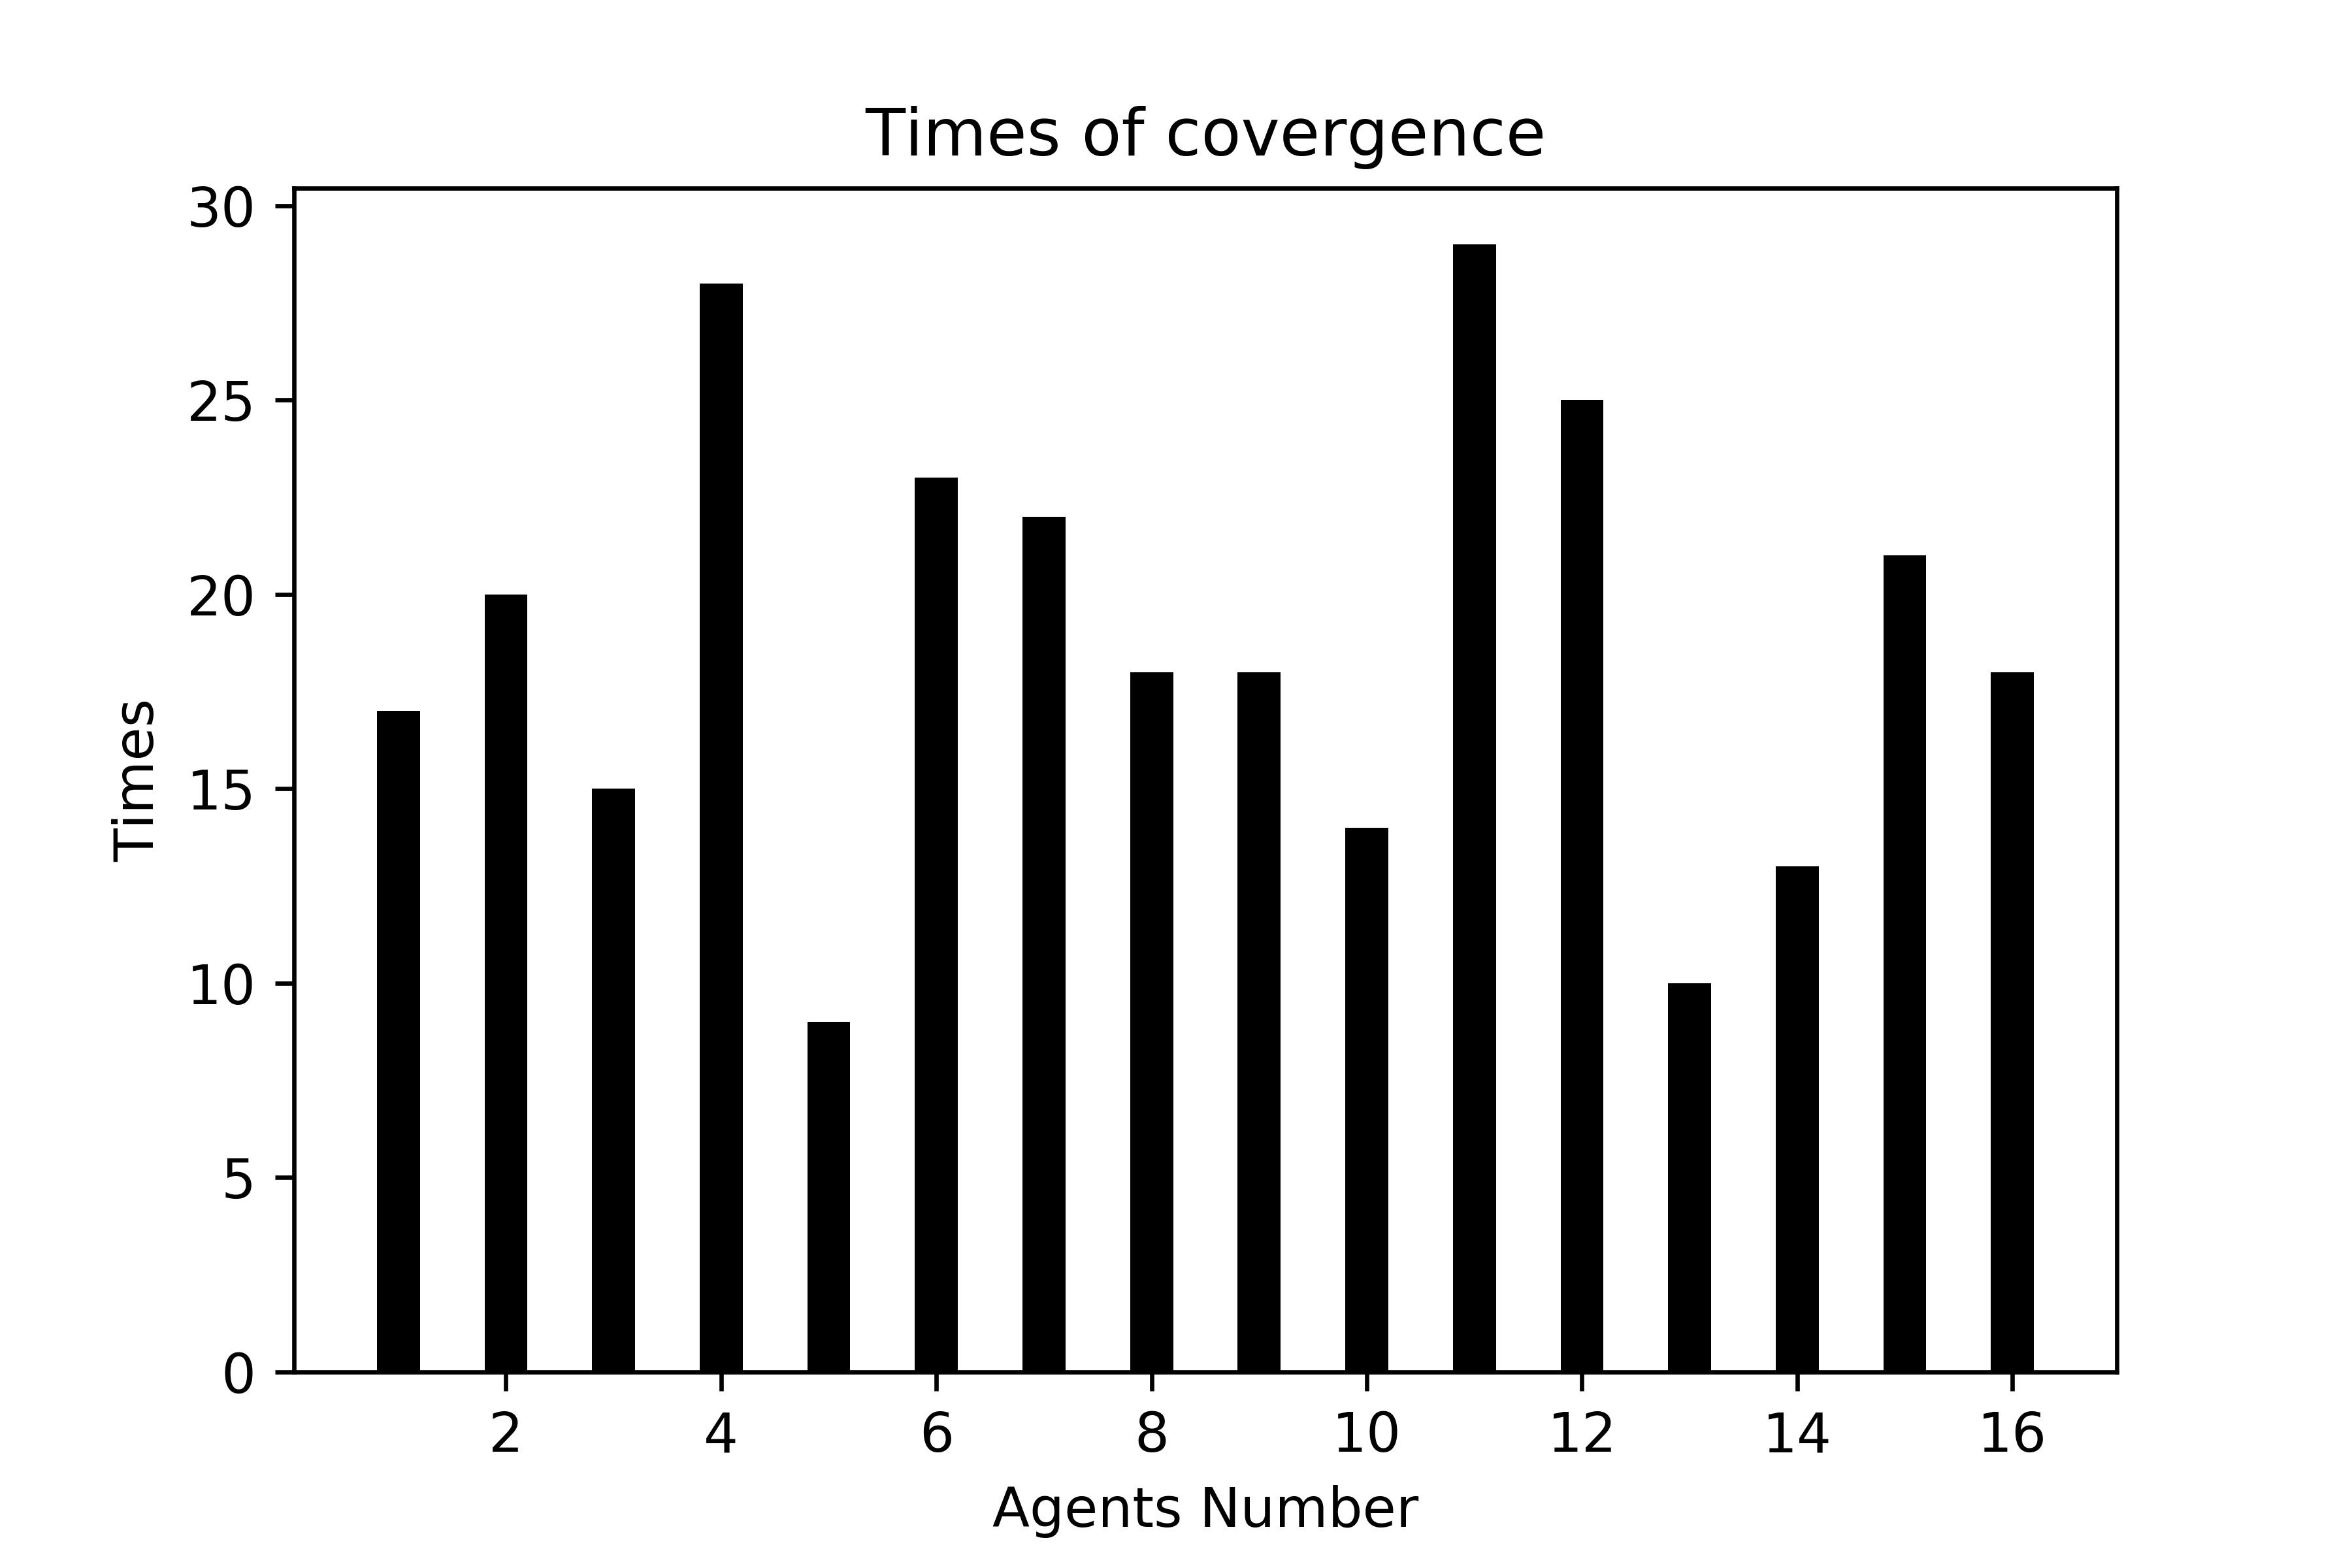
\includegraphics[width=0.9\textwidth]{agt50_4_1000_300}
    	\caption{Where the iterations converge}\label{agt50_4_1000_300}
    \end{figure}
    %
    \begin{figure}[H]
    	\centering
    	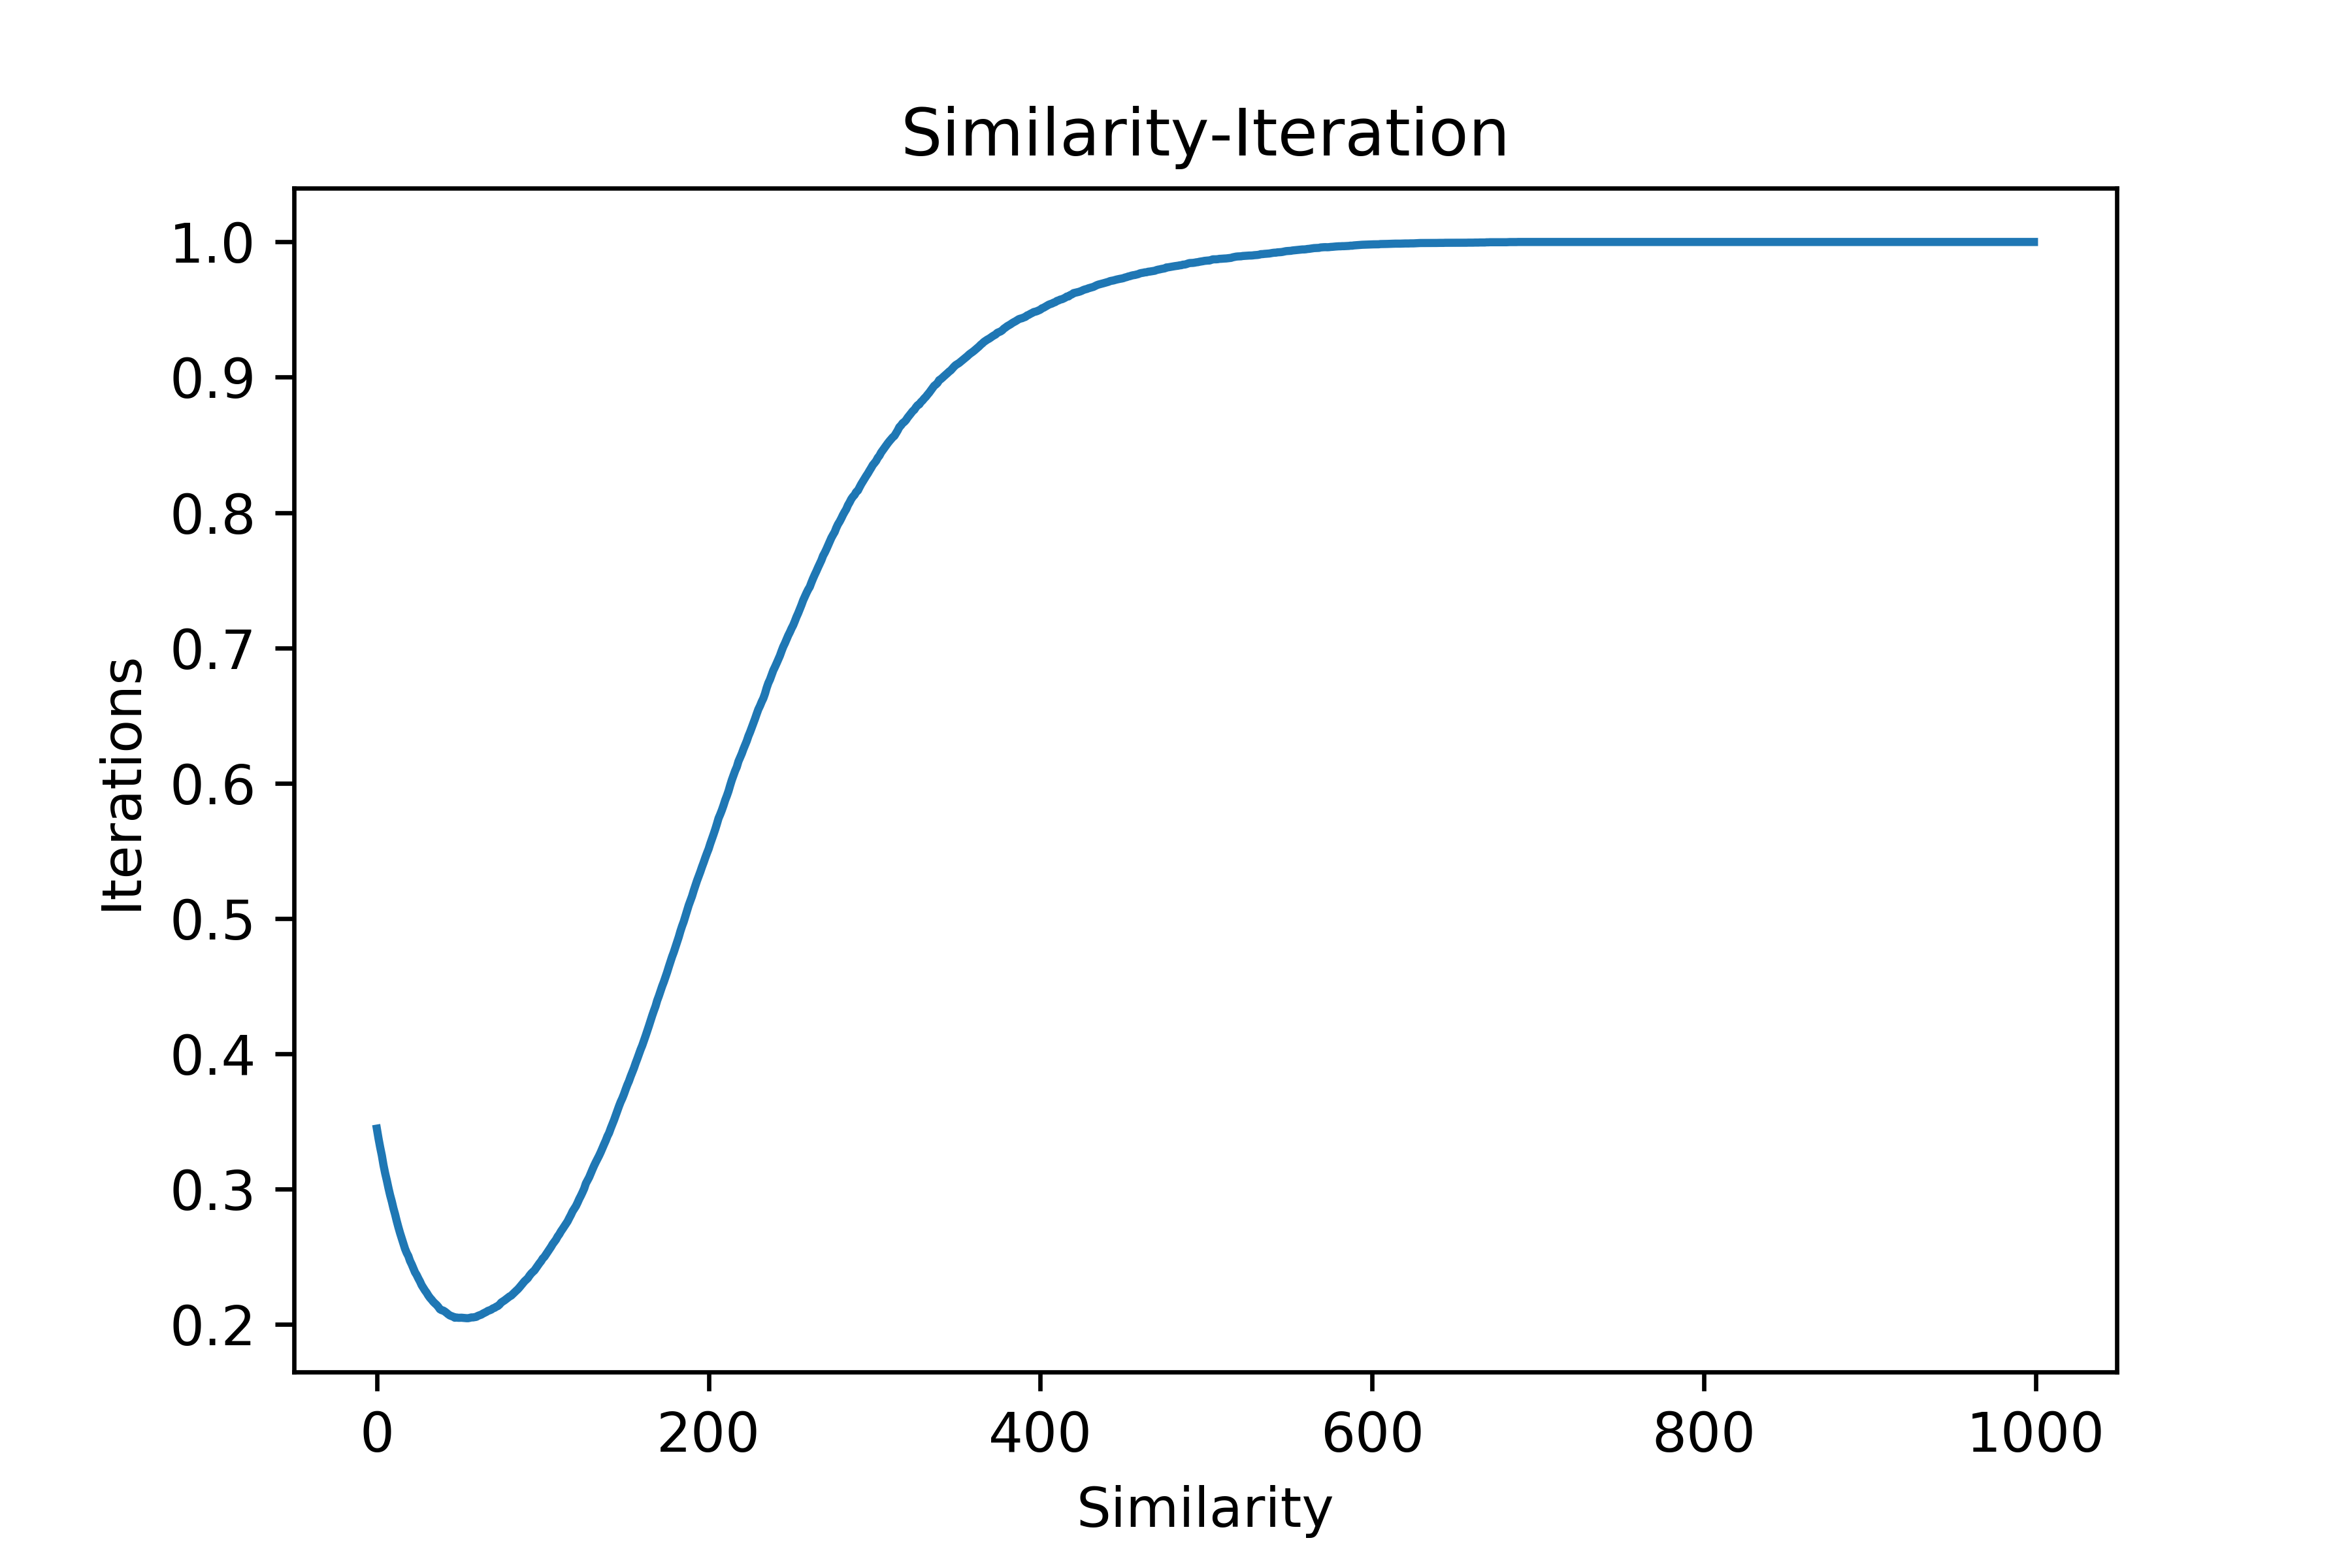
\includegraphics[width=0.9\textwidth]{Sim50_4_1000_300}
    	\caption{Similarity}\label{Sim50_4_1000_300}
    \end{figure}
    %
    \begin{figure}[H]
    	\centering
    	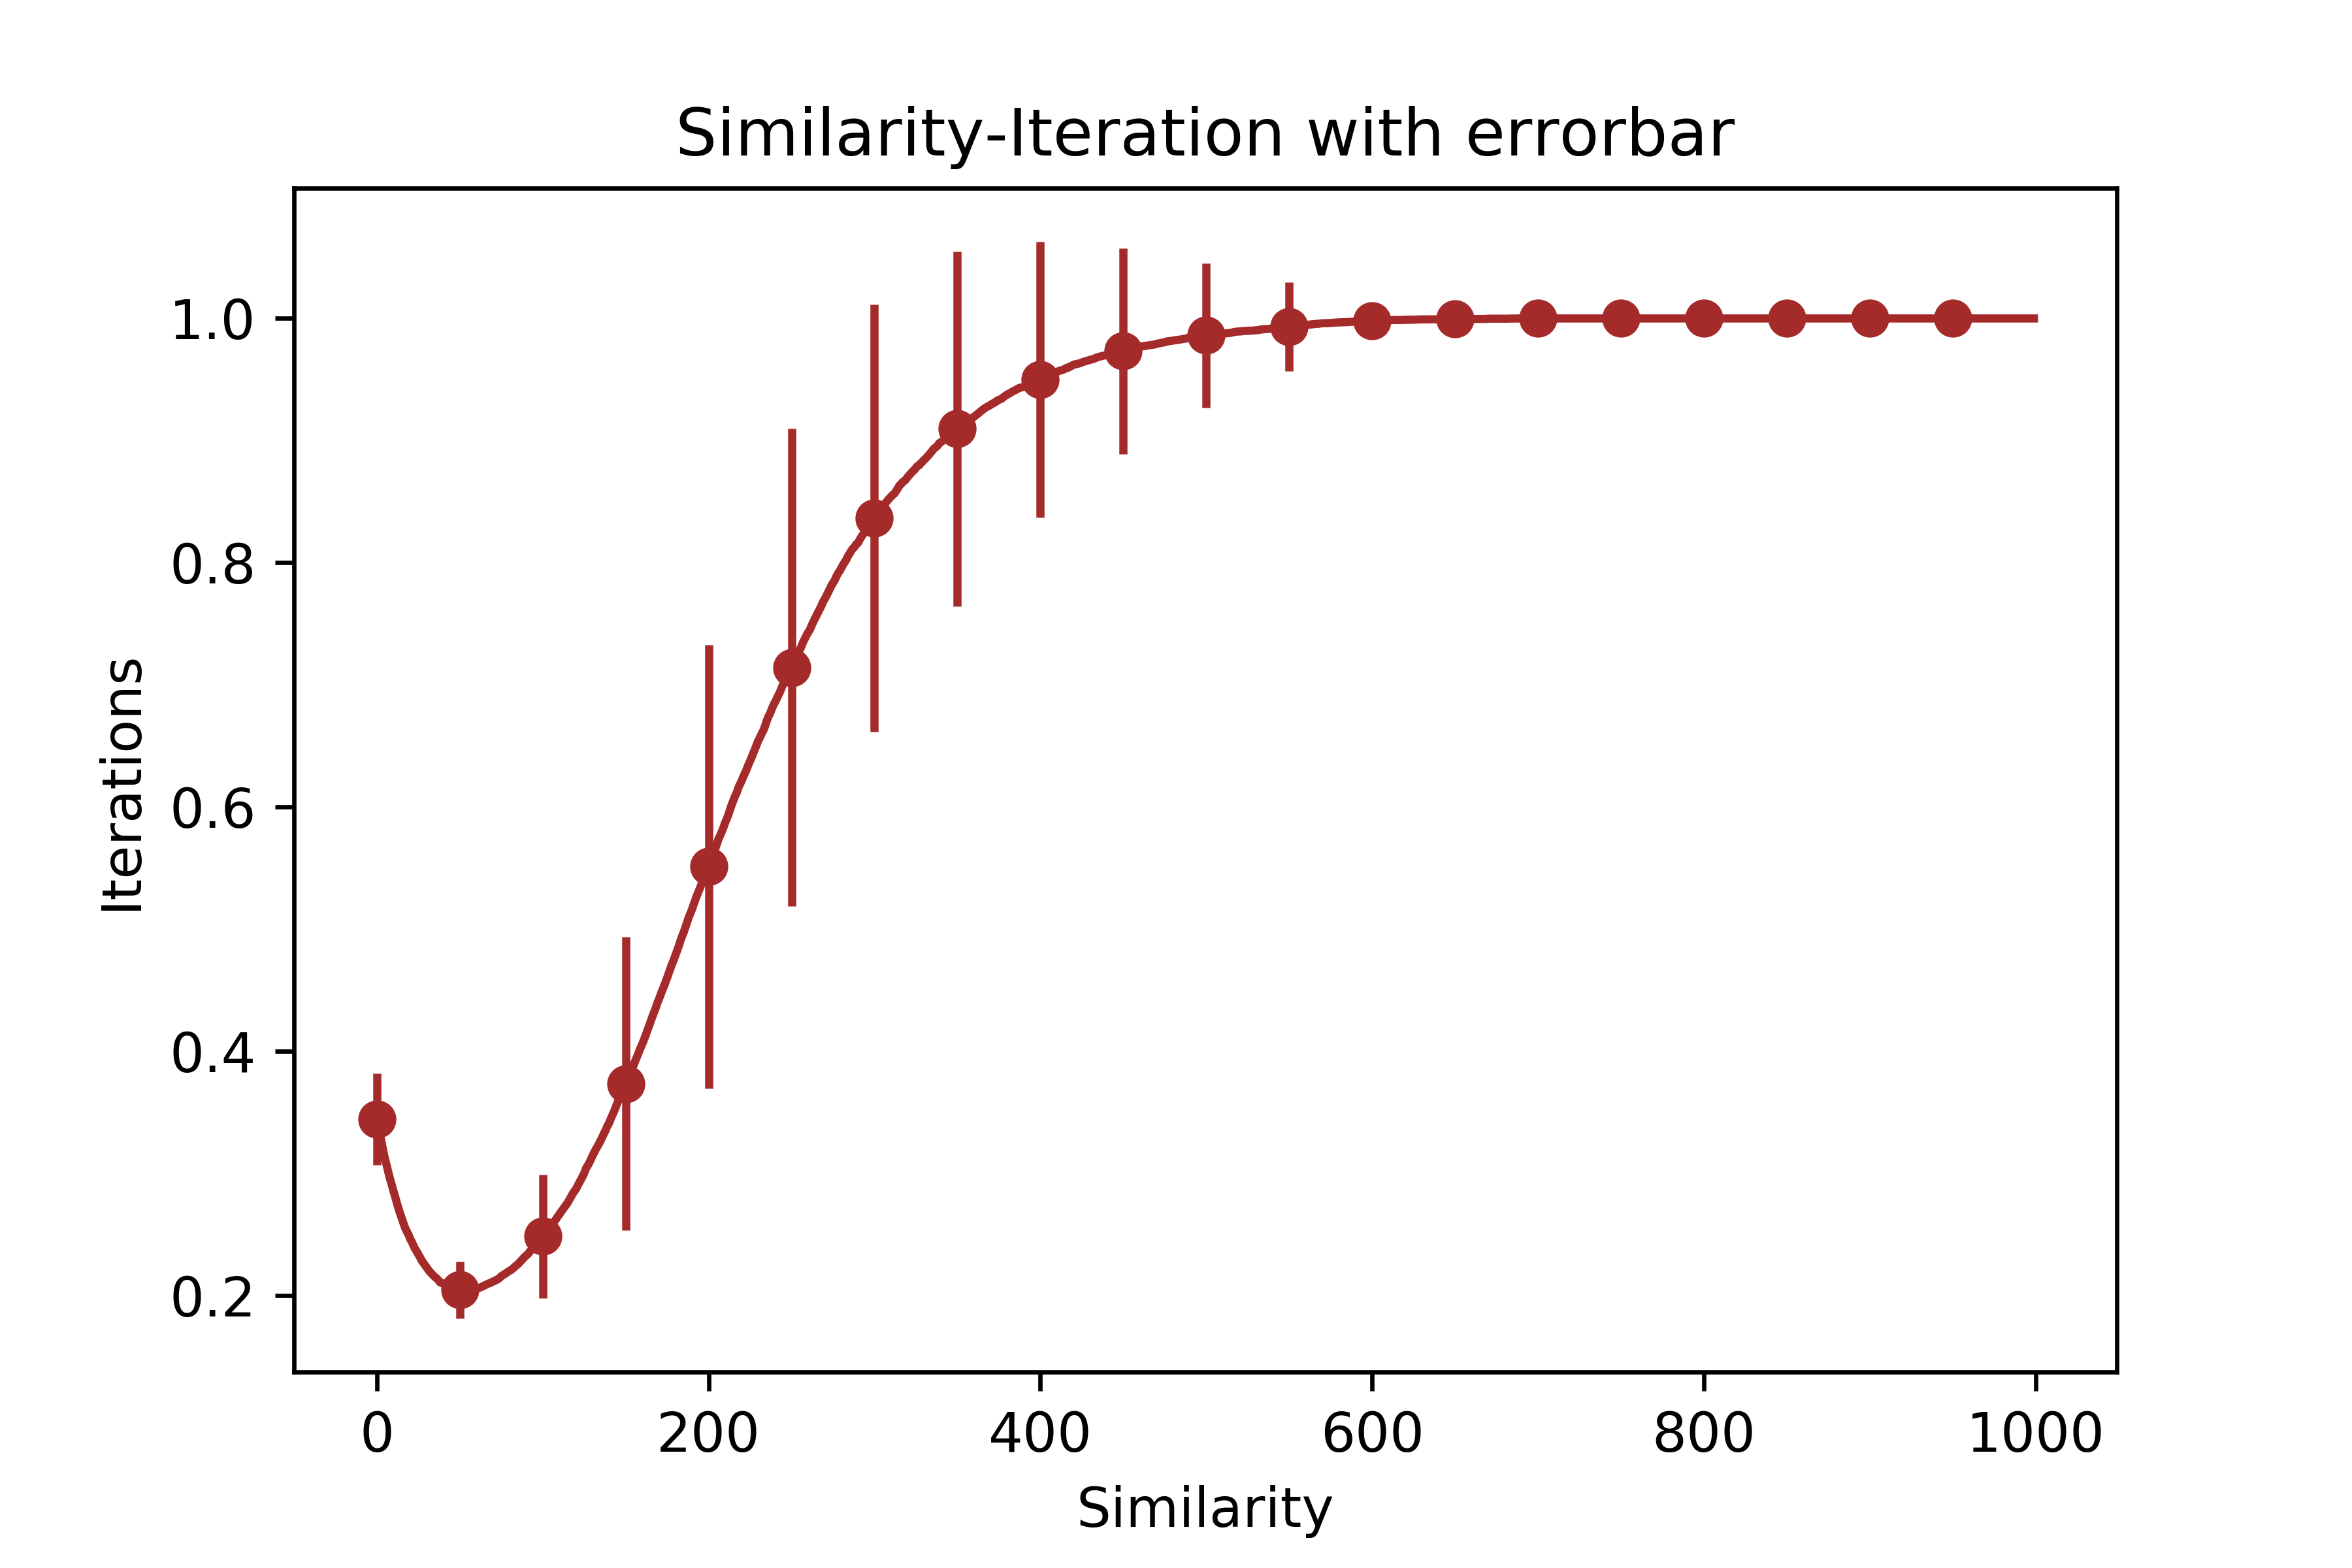
\includegraphics[width=0.9\textwidth]{SimErr50_4_1000_300}
    	\caption{Similarity with error bar}\label{SimErr50_4_1000_300}
    \end{figure}
    %
    \begin{figure}[H]
    	\centering
    	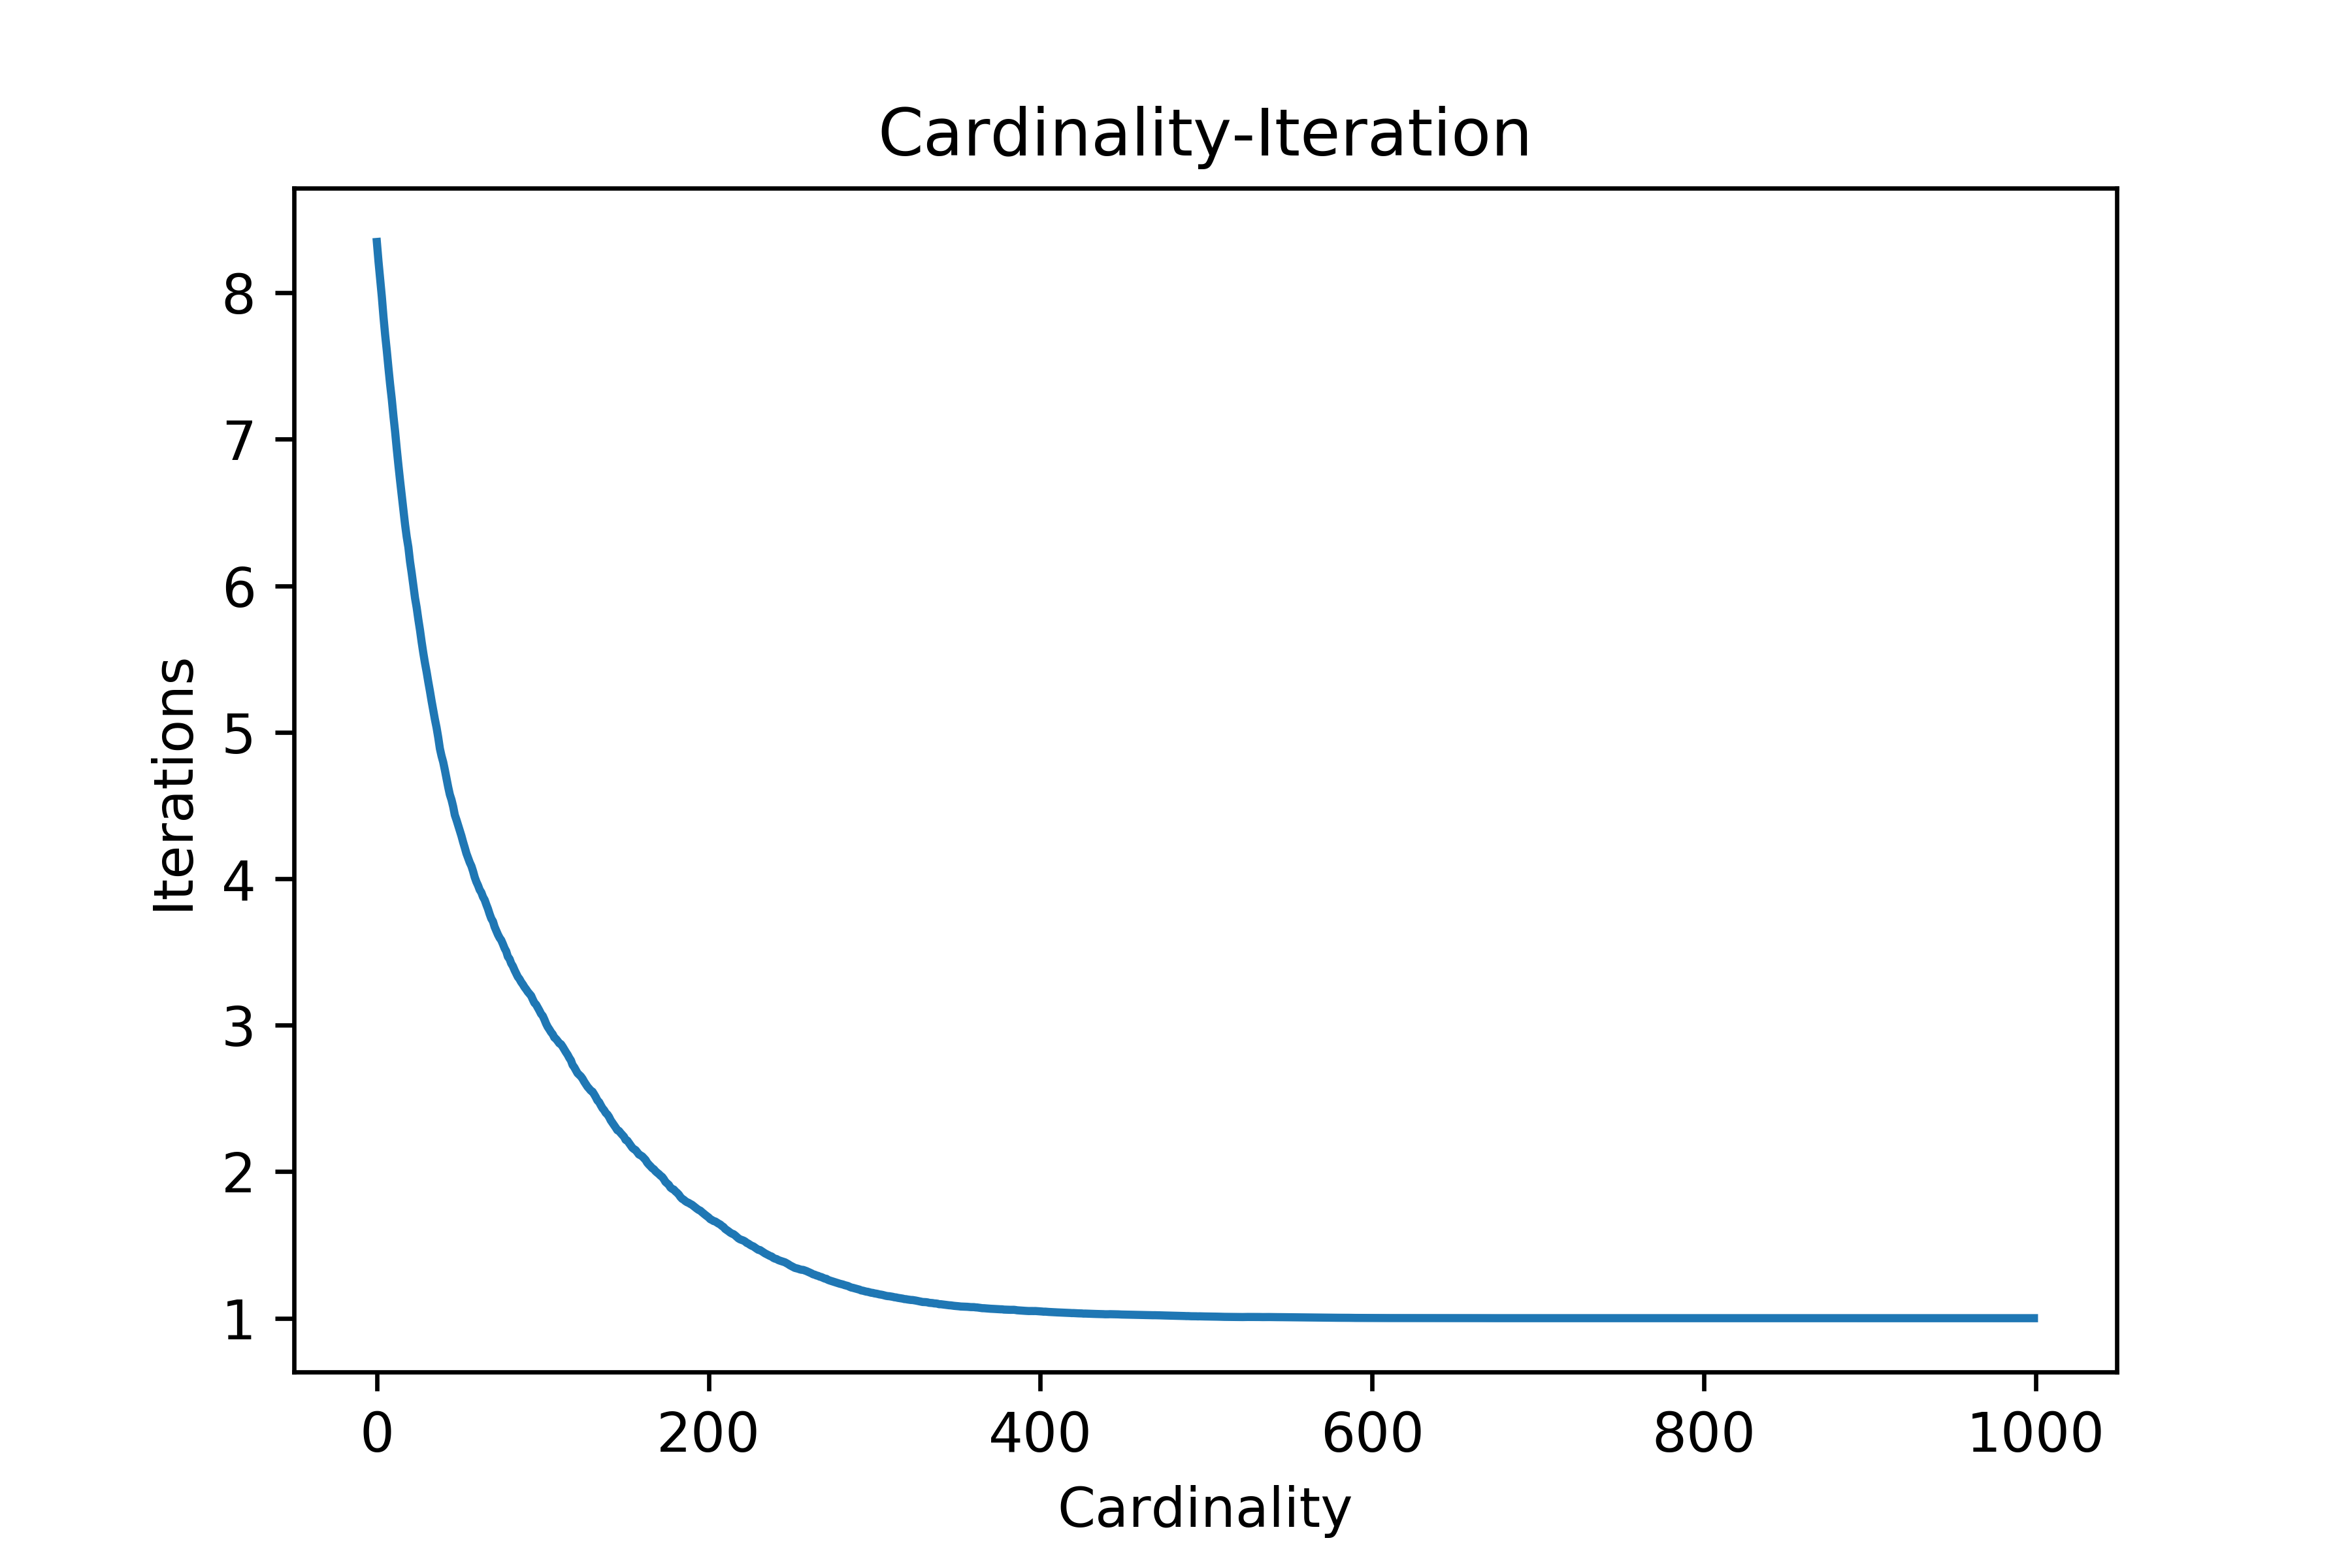
\includegraphics[width=0.9\textwidth]{Card50_4_1000_300}
    	\caption{Cardinality}\label{Card50_4_1000_300}
    \end{figure}
    %
    \begin{figure}[H]
    	\centering
    	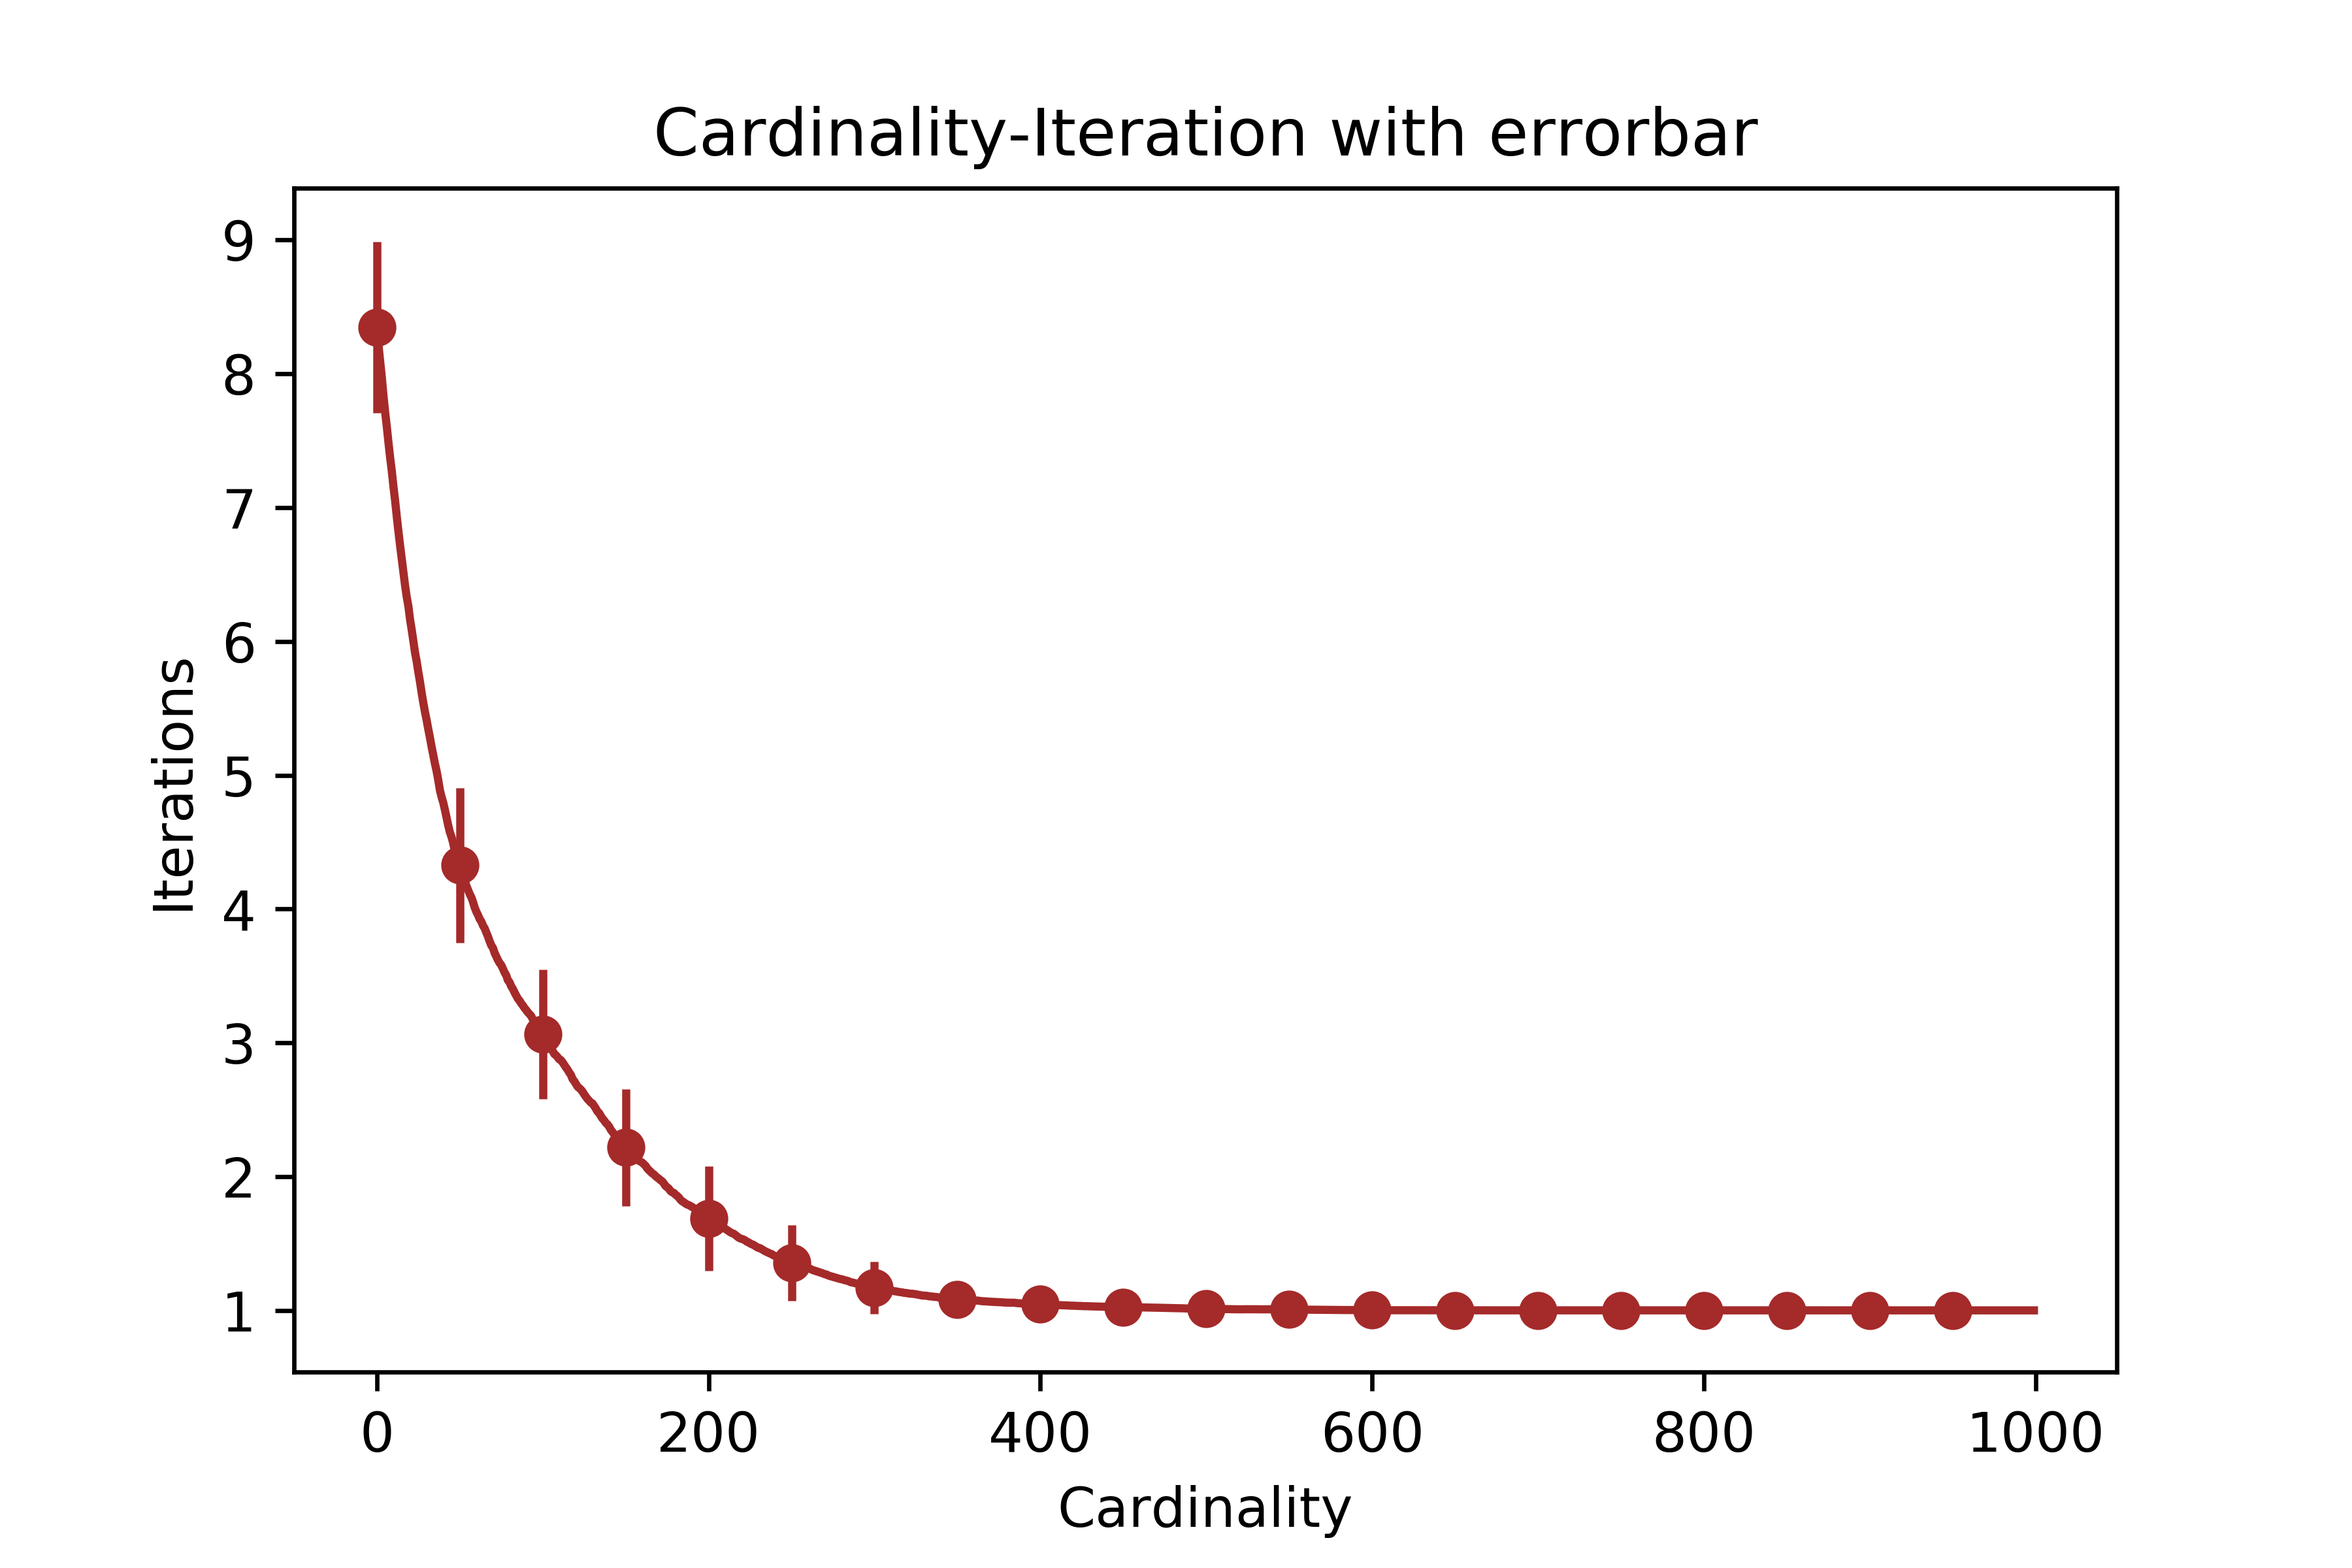
\includegraphics[width=0.9\textwidth]{CardErr50_4_1000_300}
    	\caption{Cardinality with error bar}\label{CardErr50_4_1000_300}
    \end{figure}
    \subsection{50\_4\_1000\_800}
    Time used: 726.9702704230385
        	\begin{figure}[H]
    	\centering
    	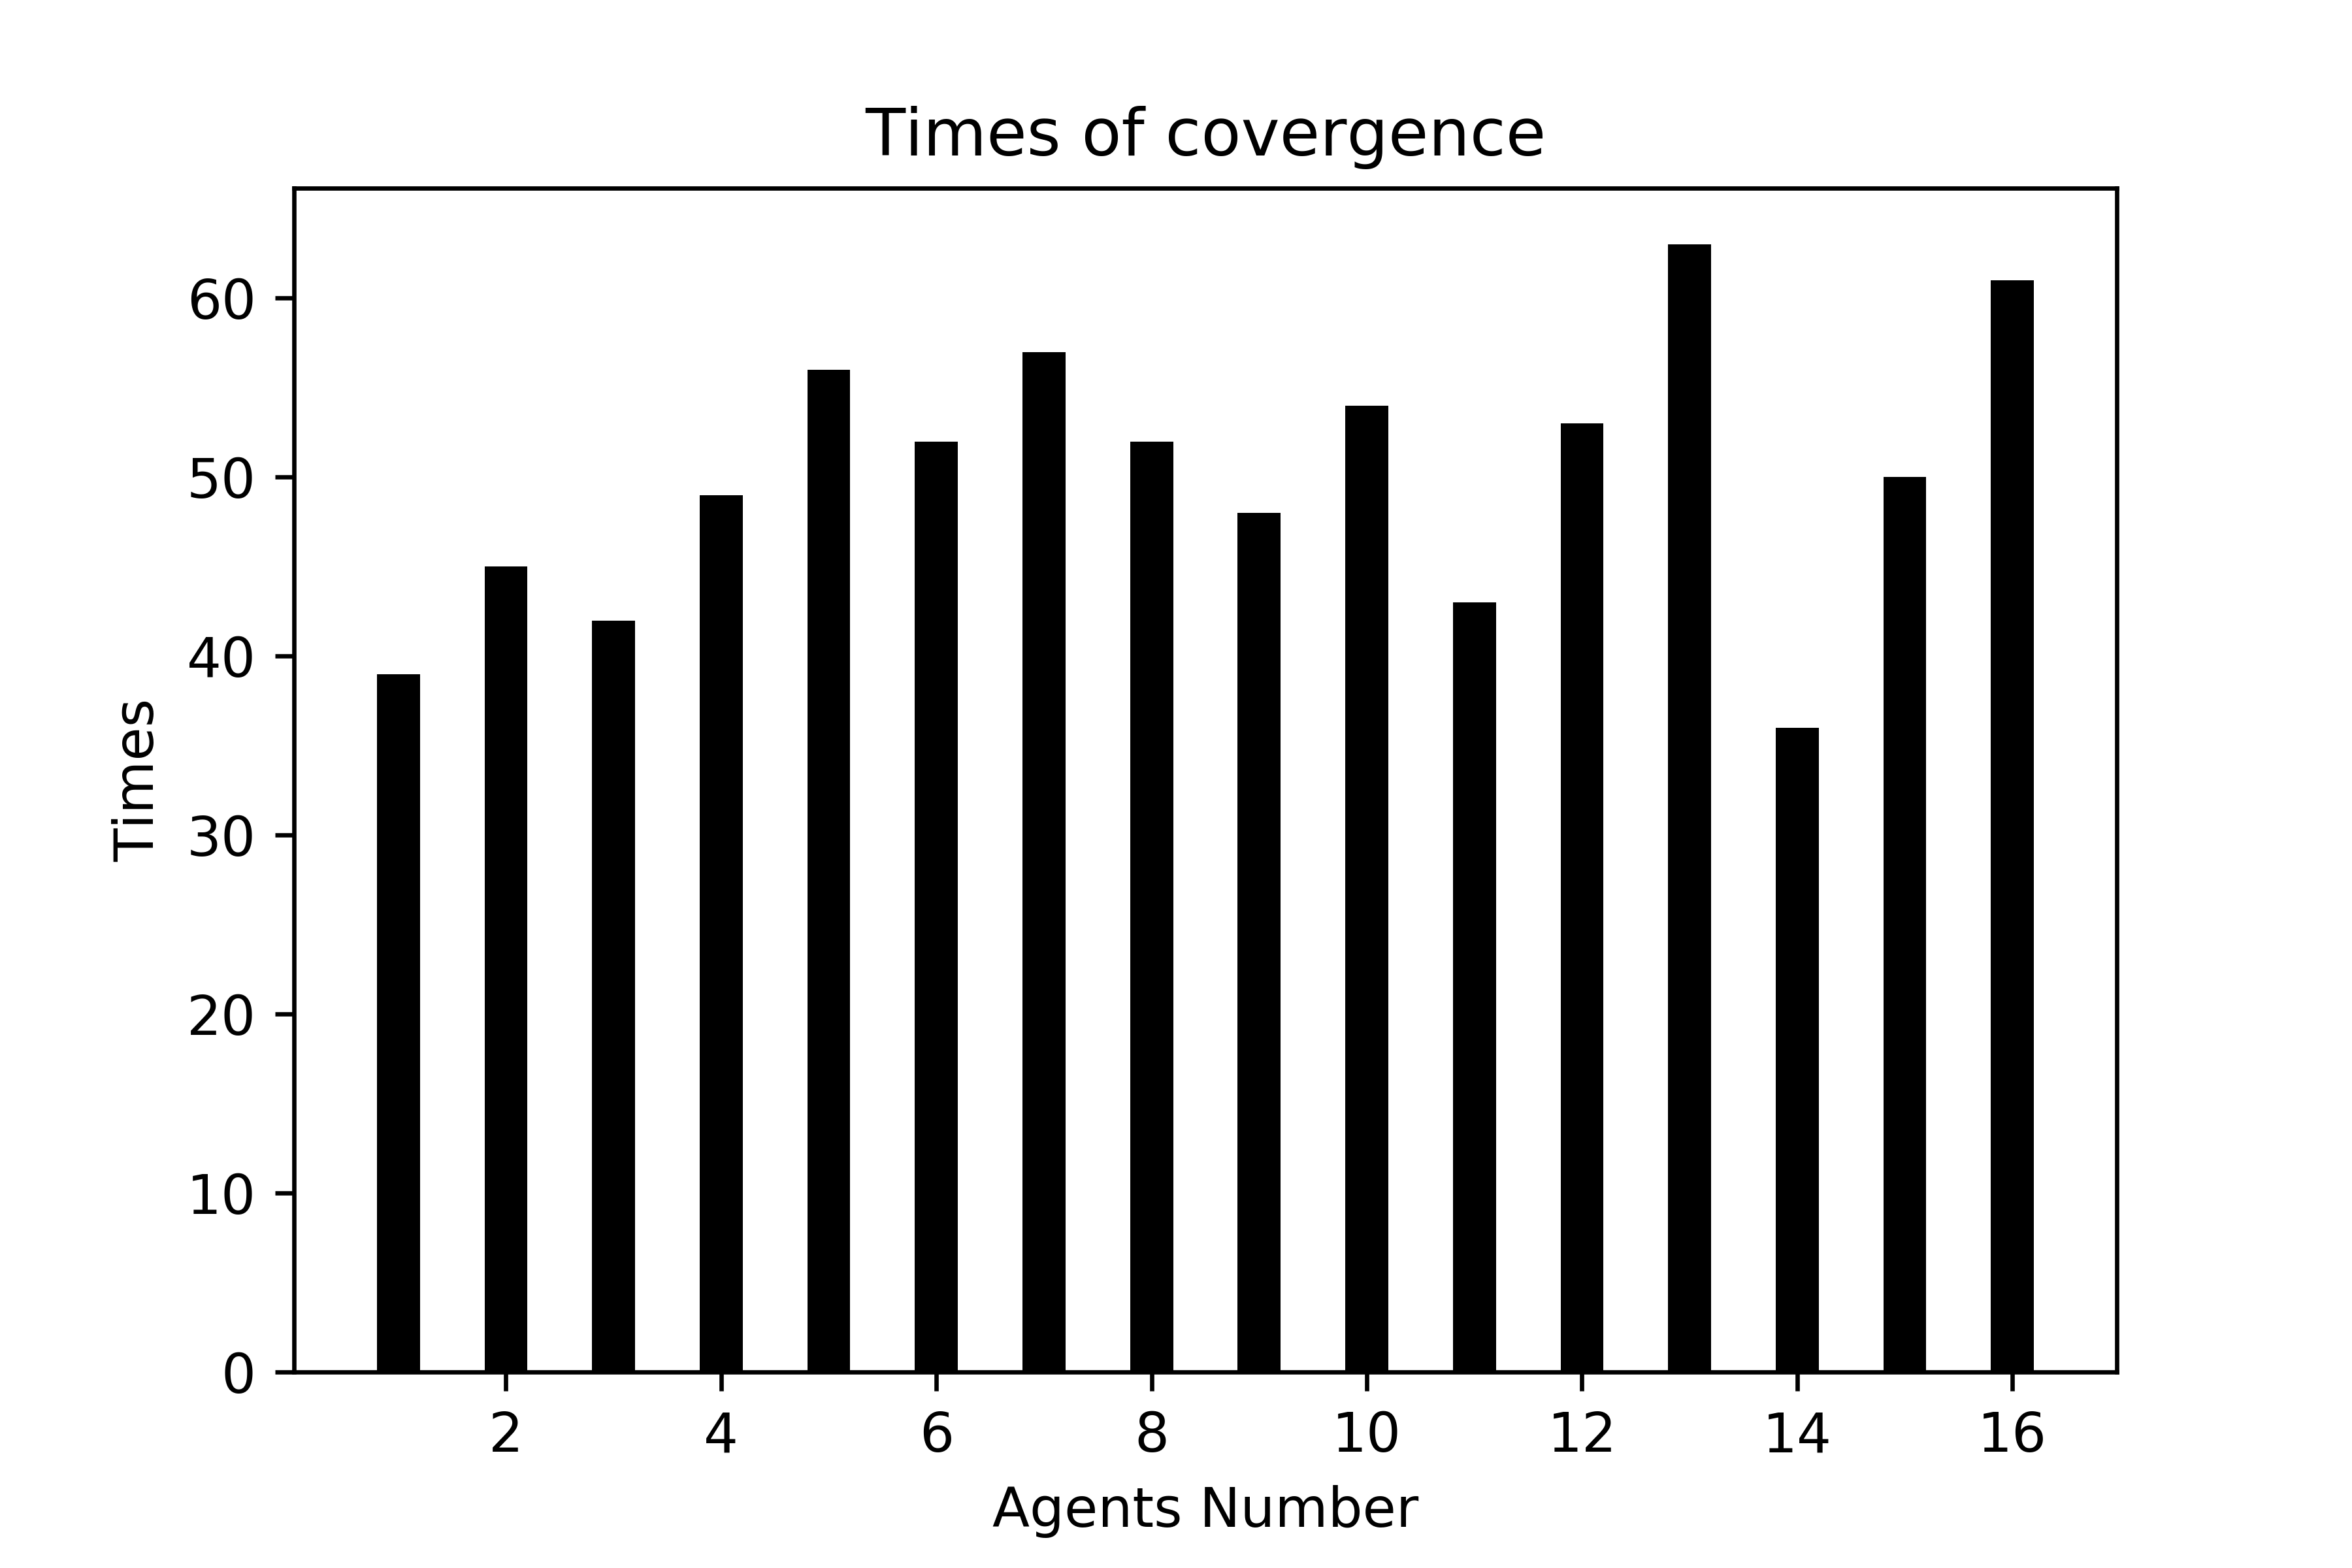
\includegraphics[width=0.9\textwidth]{agt50_4_1000_800}
    	\caption{Where the iterations converge}\label{agt50_4_1000_800}
    \end{figure}
    %
    \begin{figure}[H]
    	\centering
    	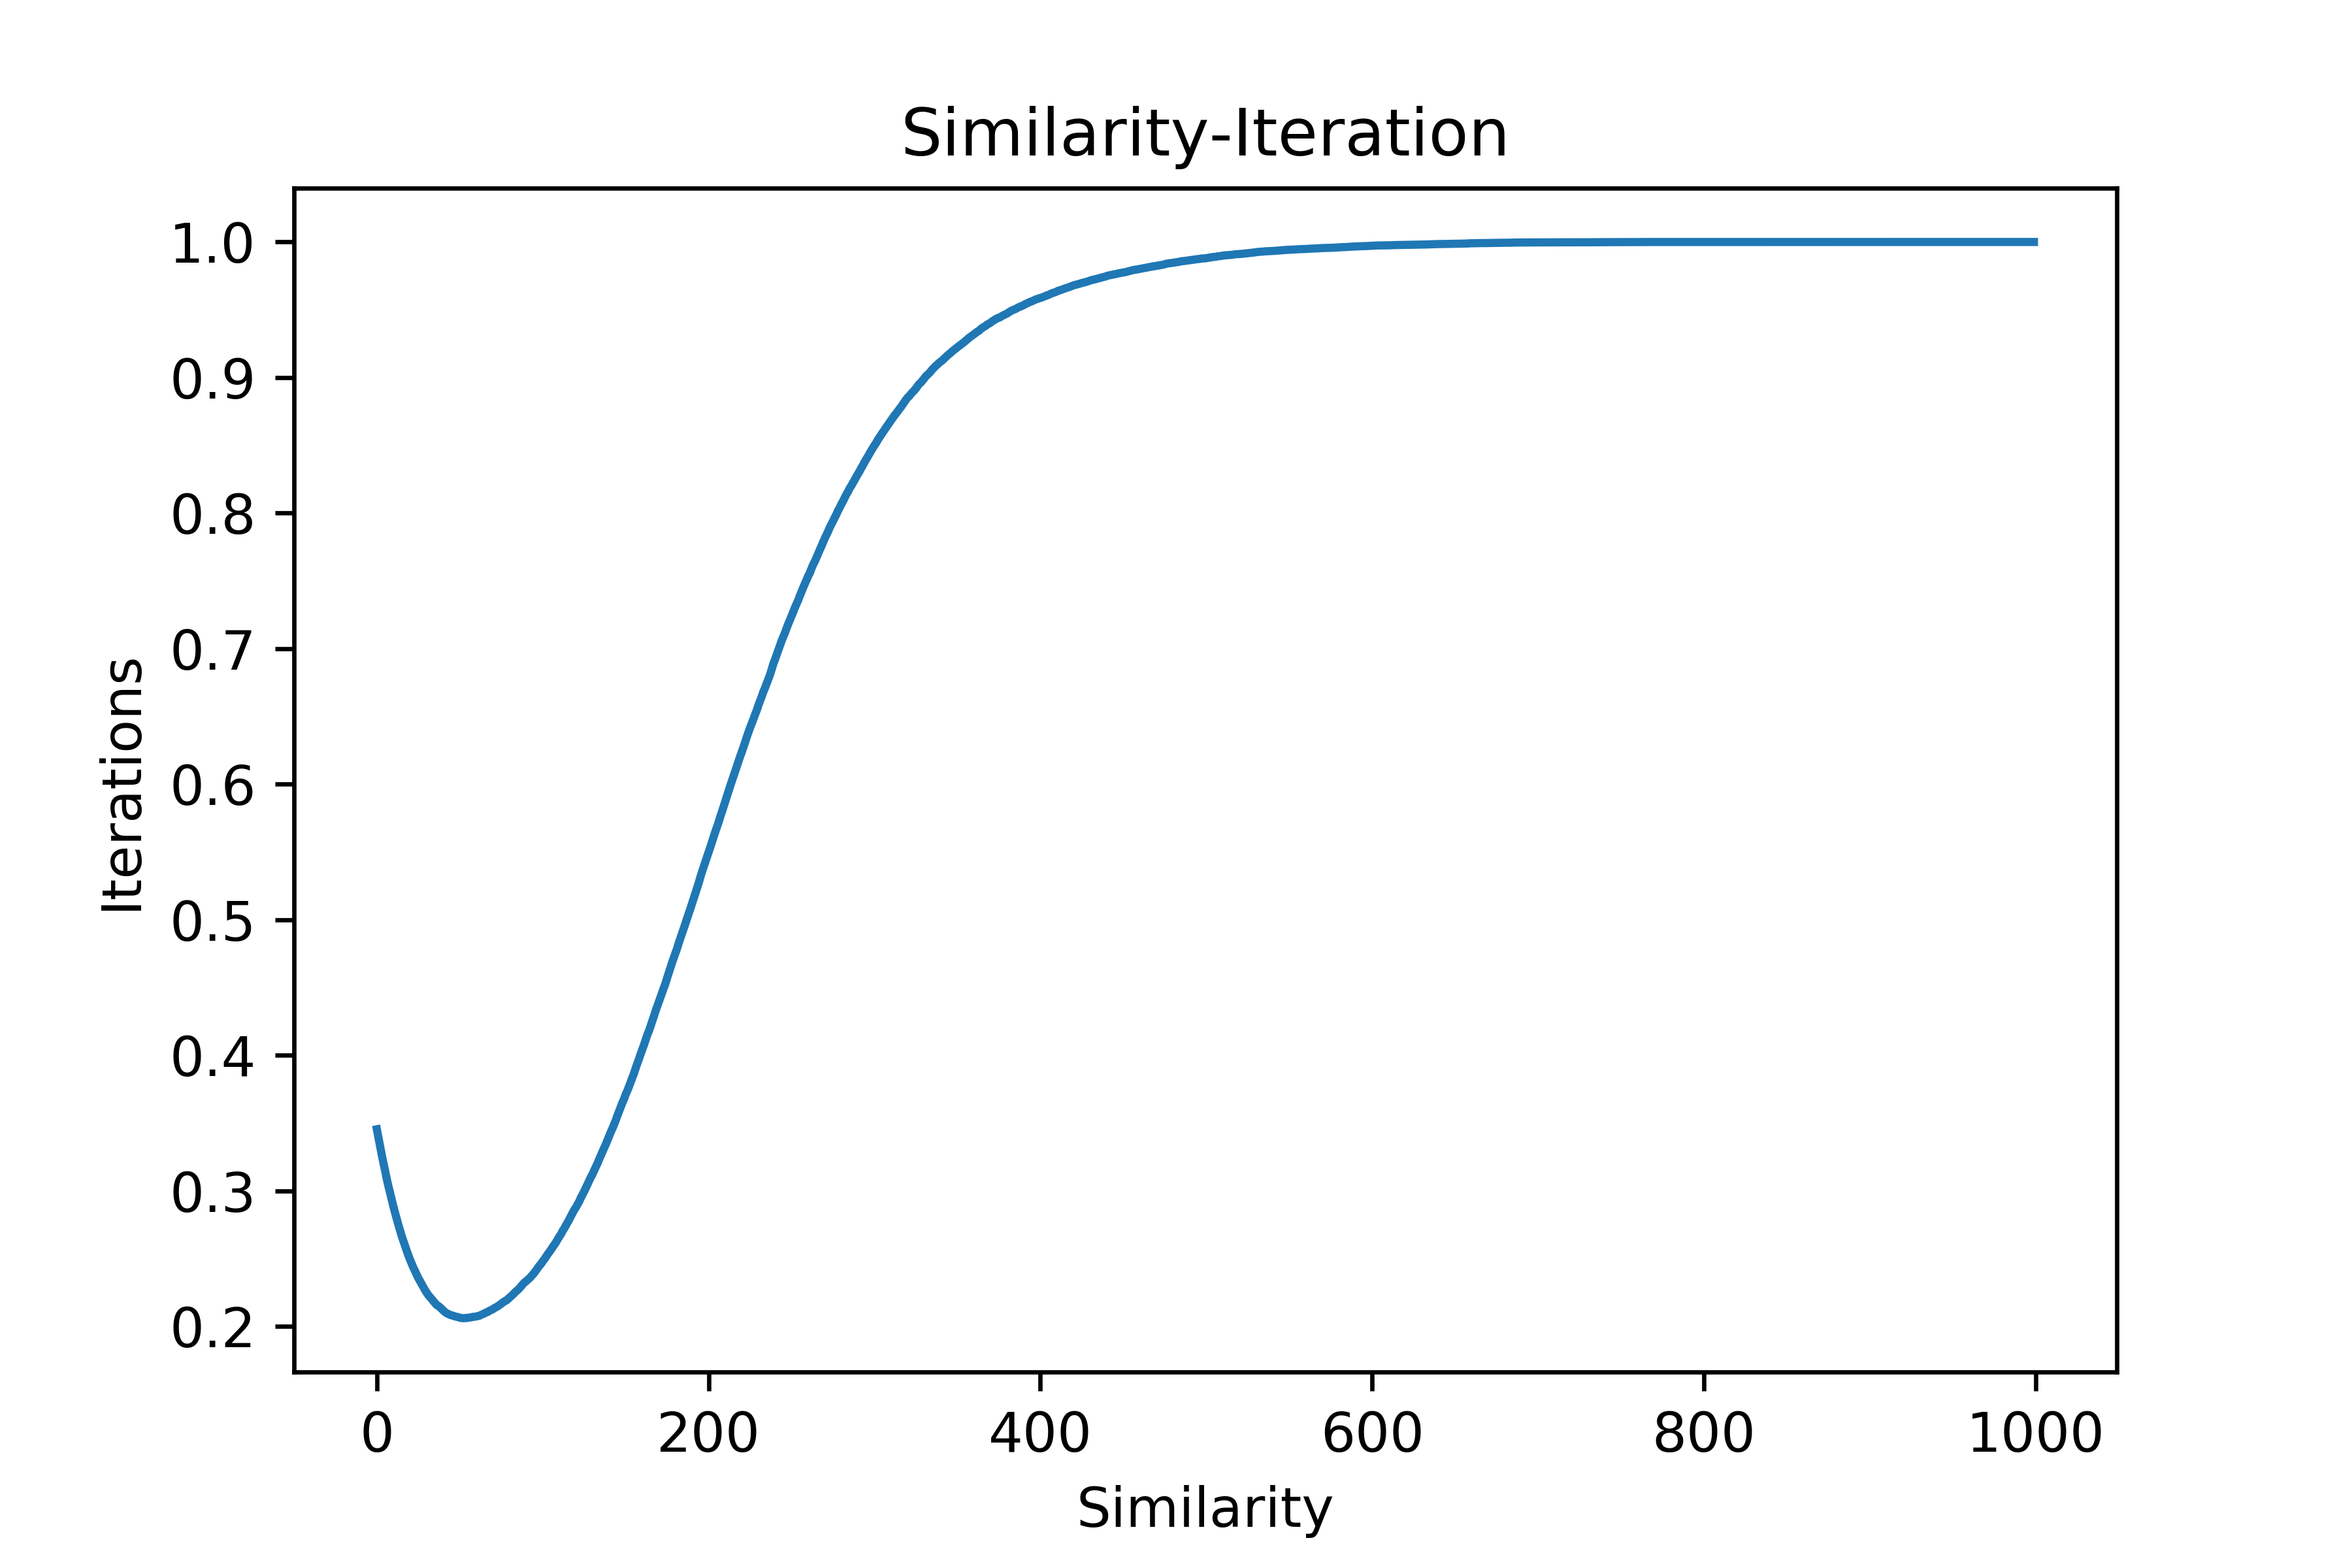
\includegraphics[width=0.9\textwidth]{Sim50_4_1000_800}
    	\caption{Similarity}\label{Sim50_4_1000_800}
    \end{figure}
    %
    \begin{figure}[H]
    	\centering
    	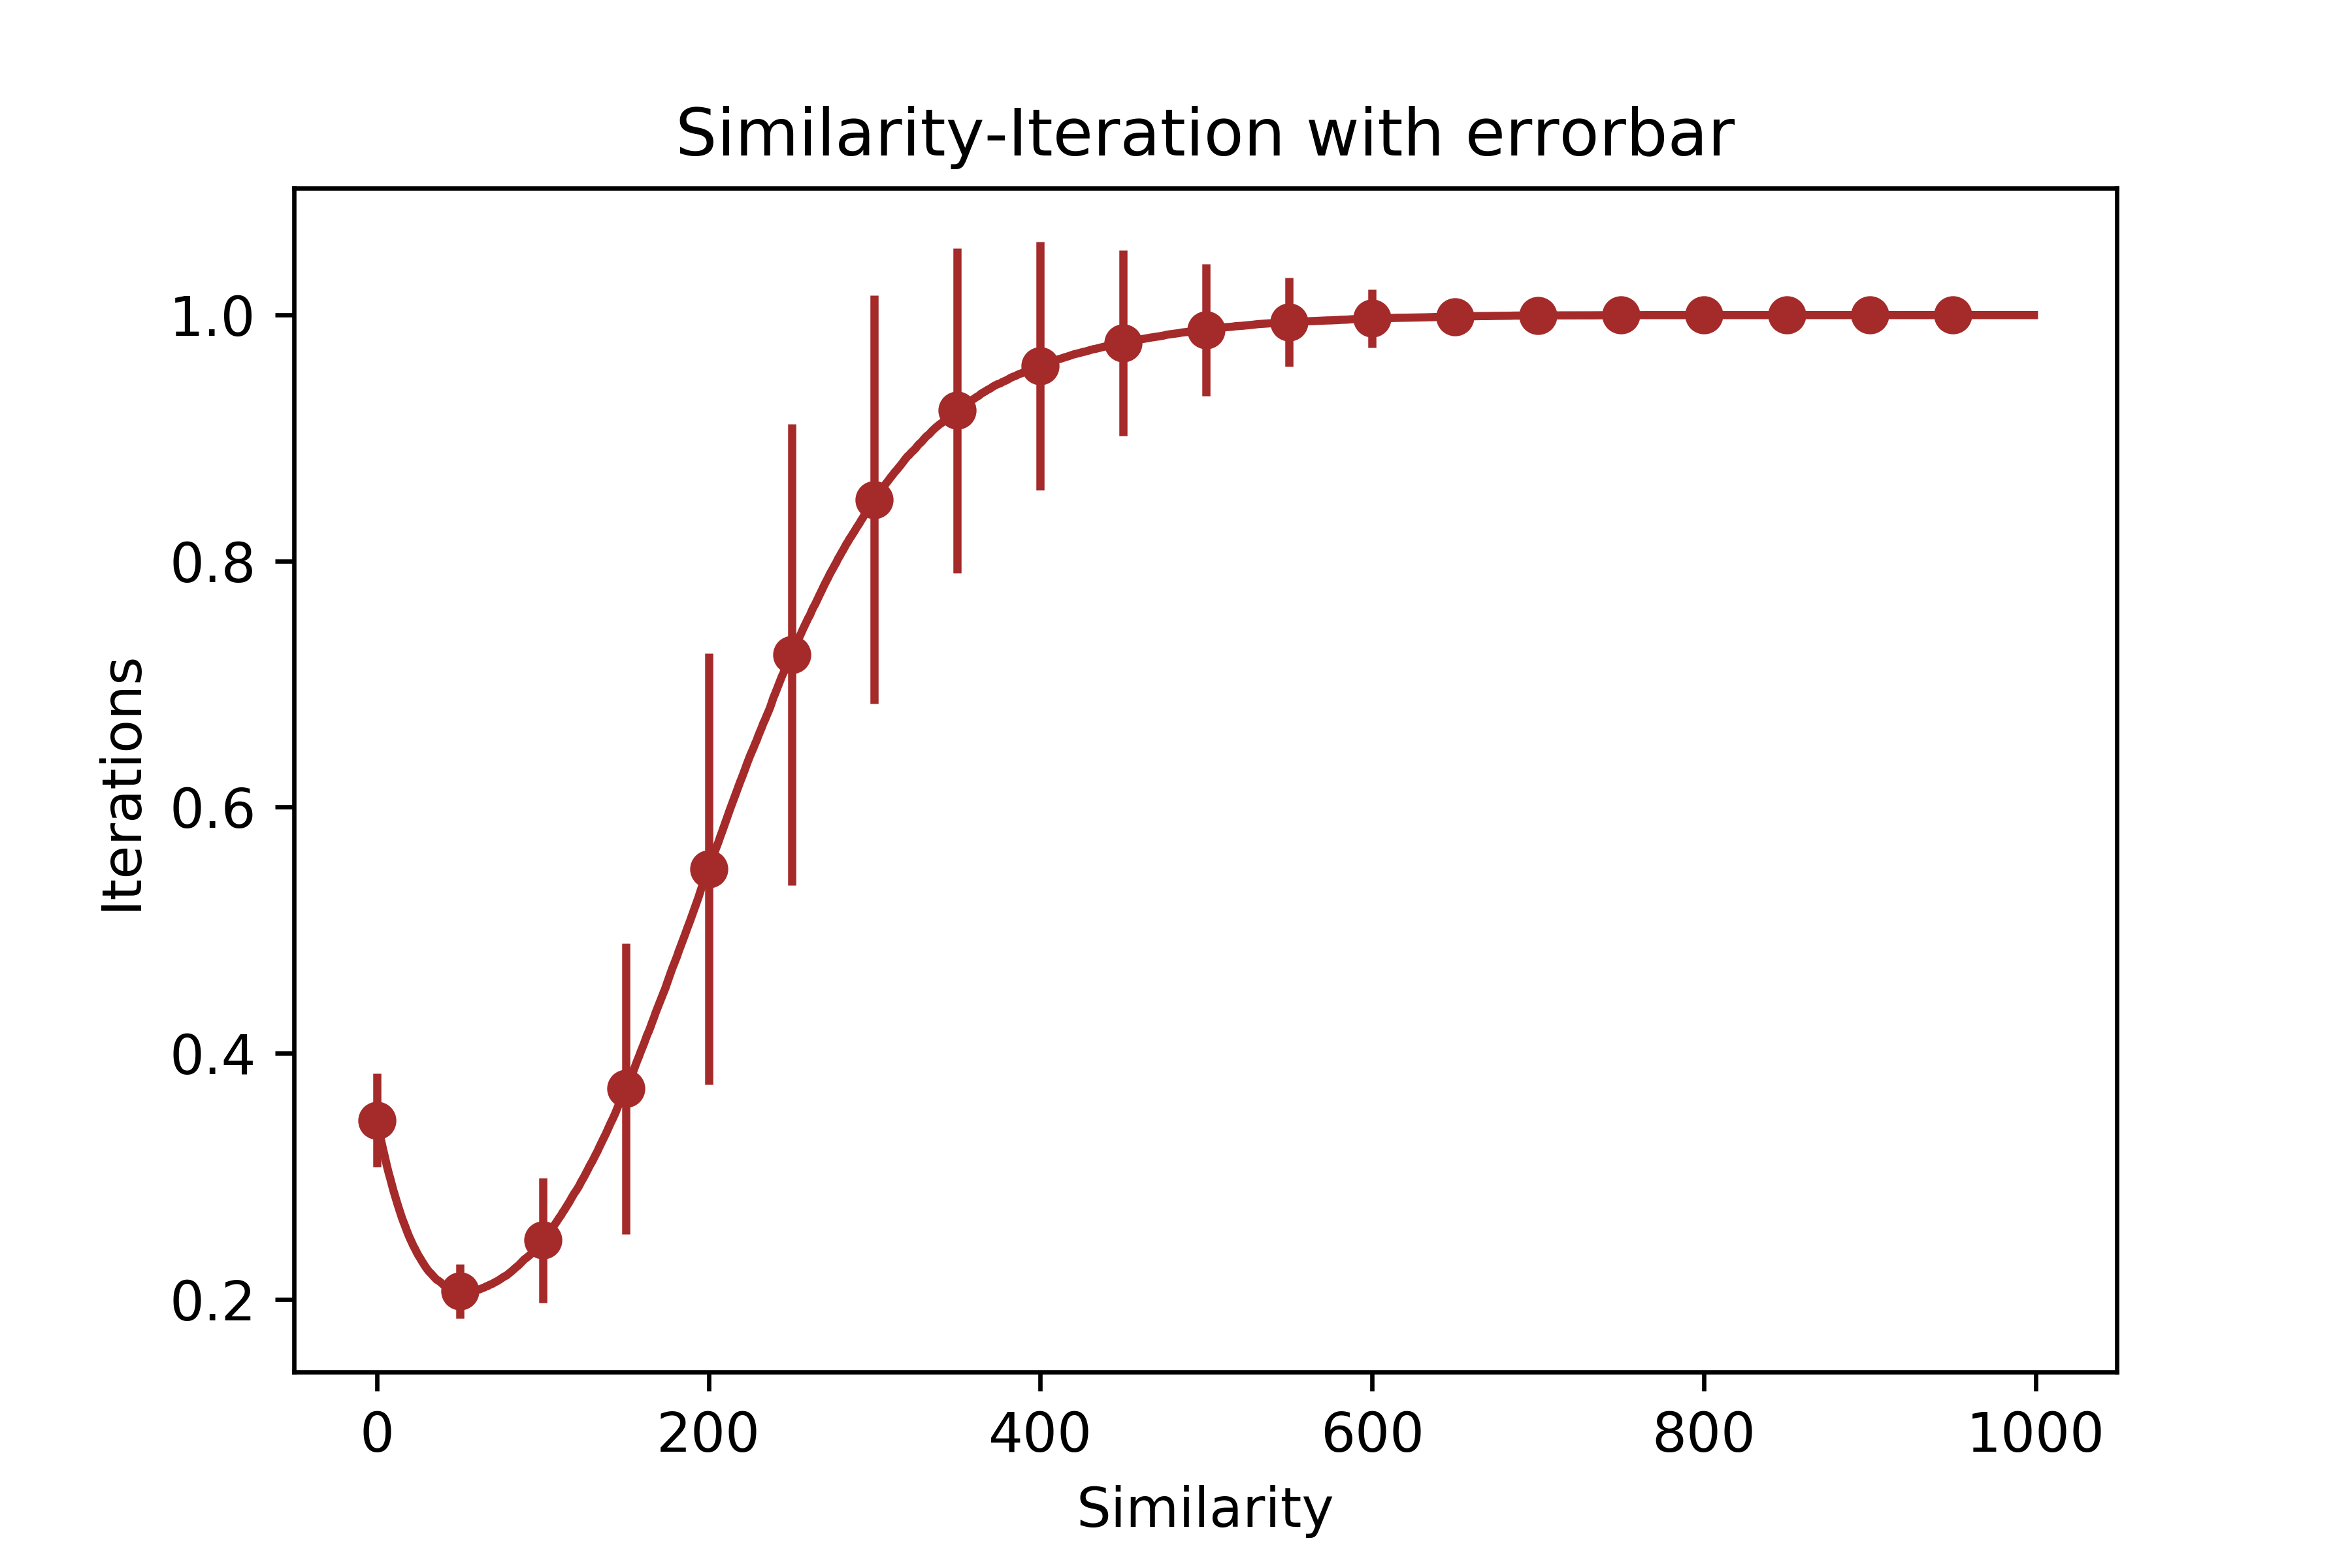
\includegraphics[width=0.9\textwidth]{SimErr50_4_1000_800}
    	\caption{Similarity with error bar}\label{SimErr50_4_1000_800}
    \end{figure}
    %
    \begin{figure}[H]
    	\centering
    	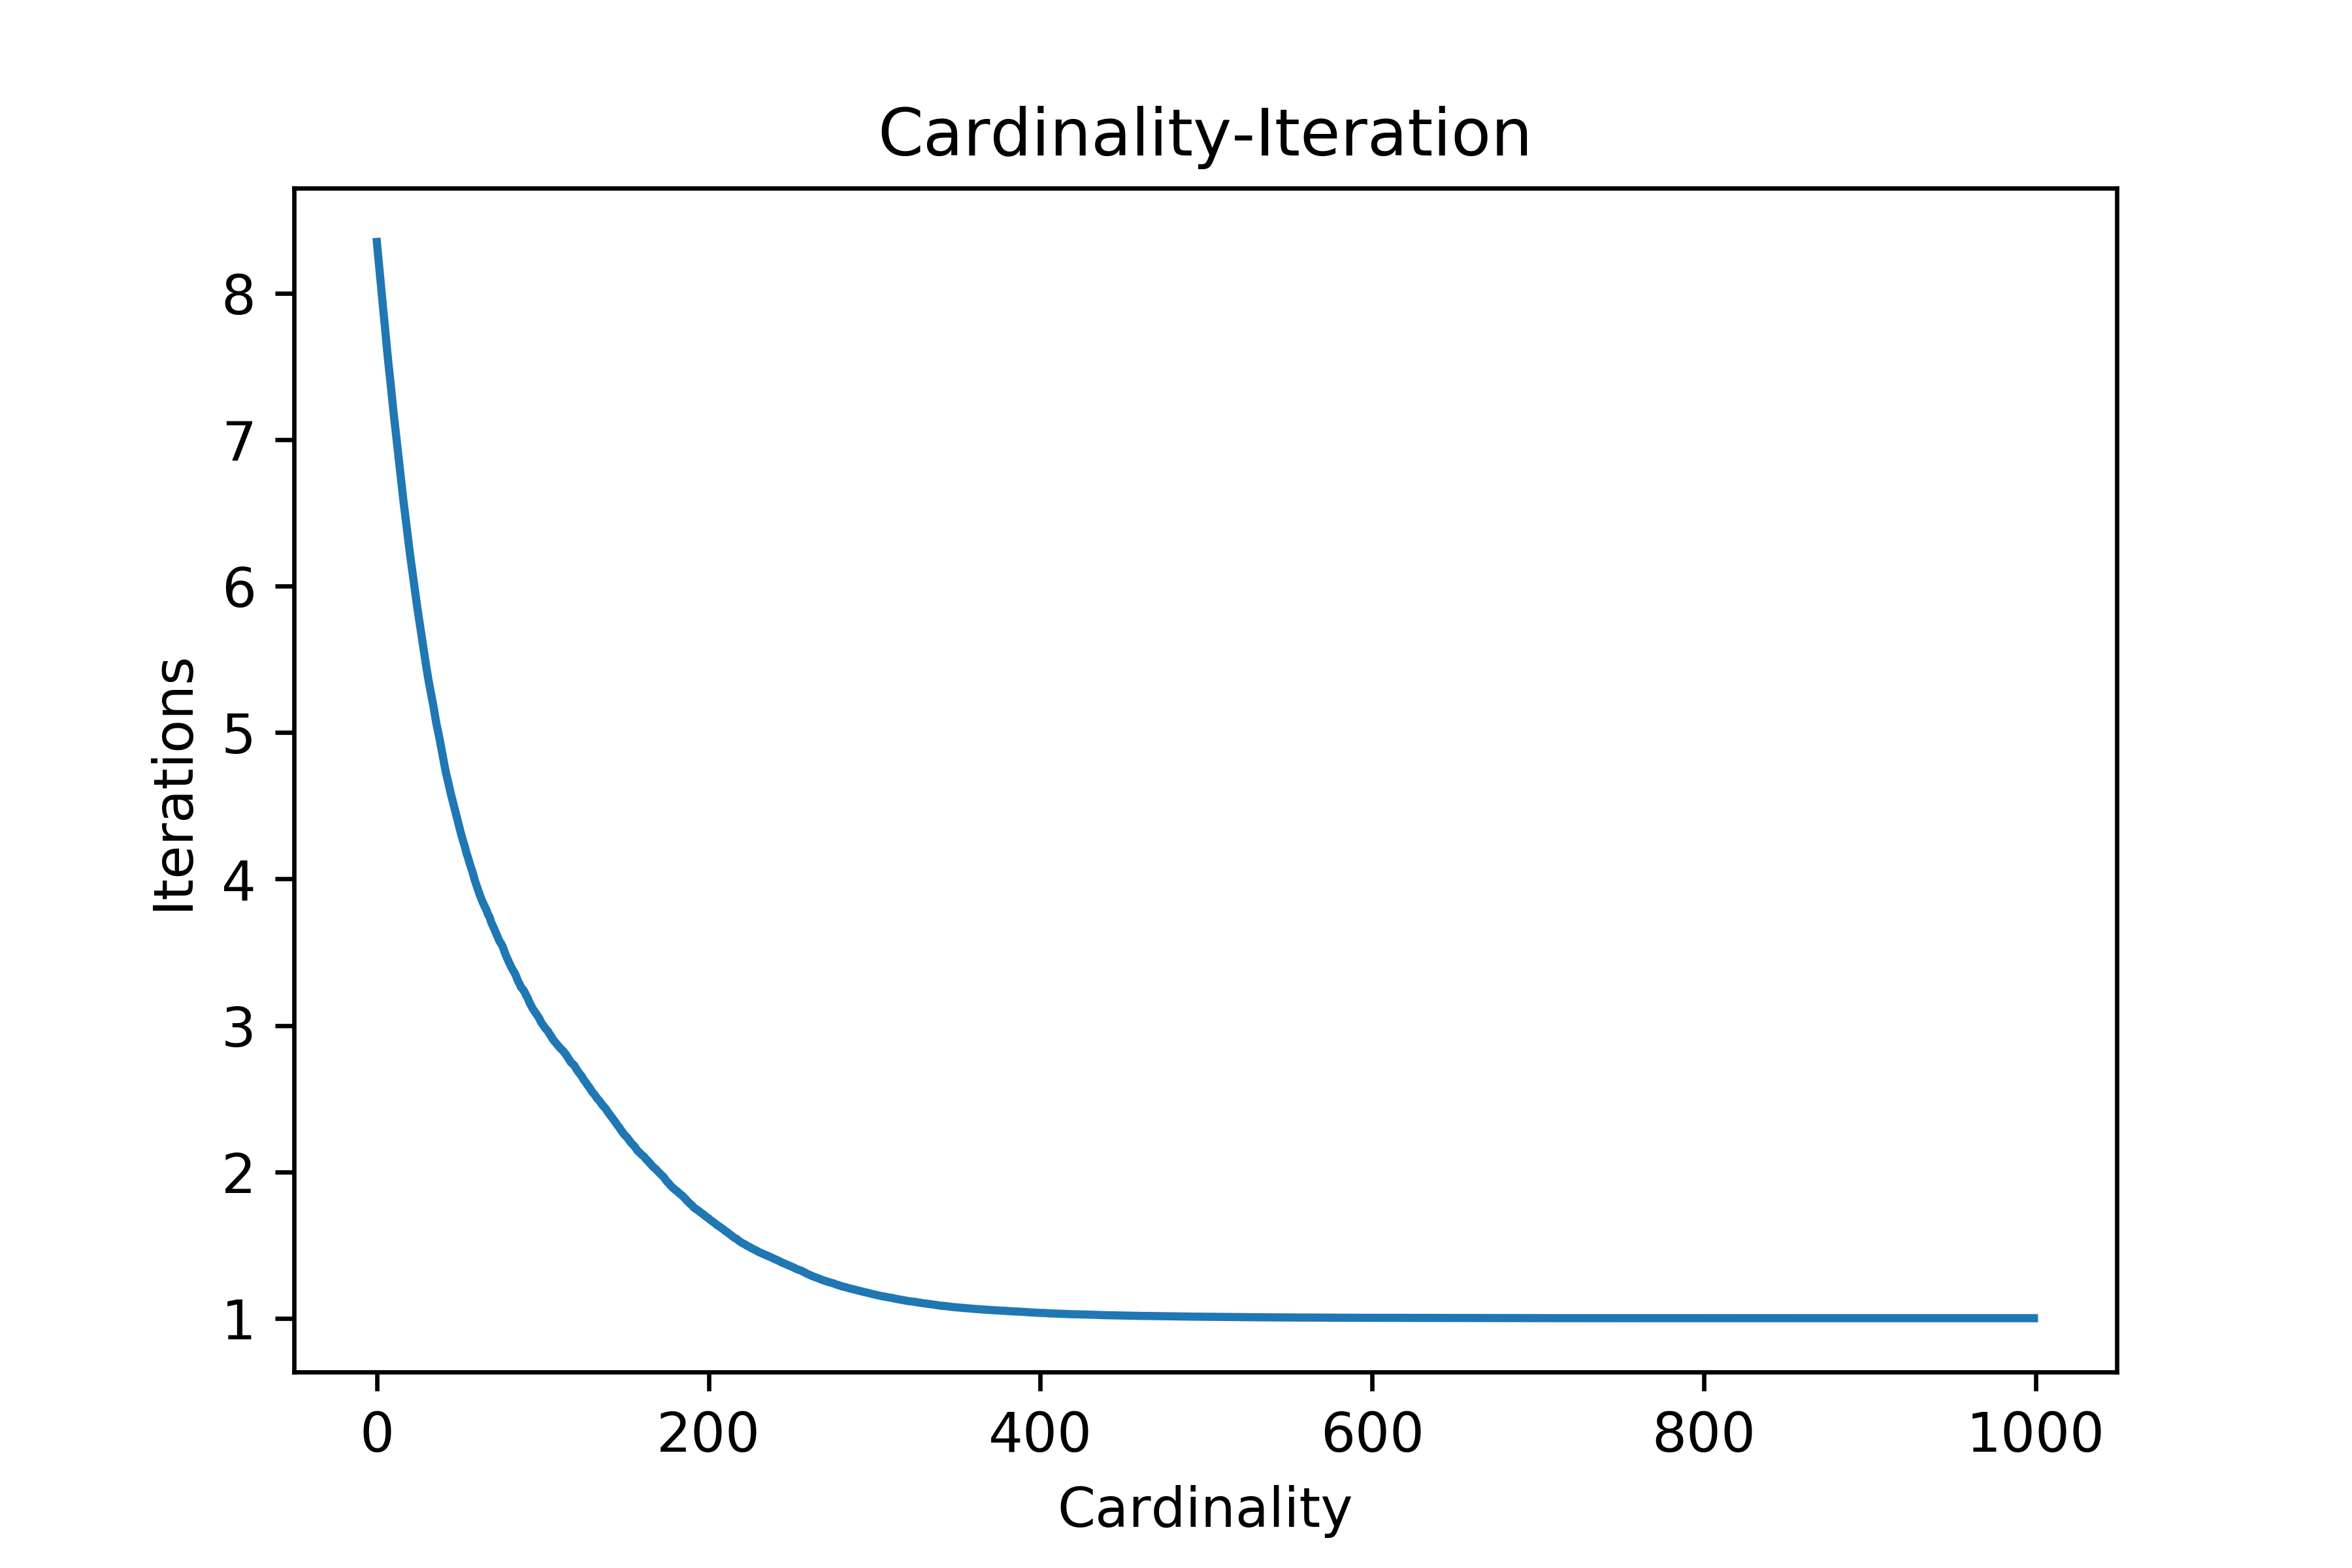
\includegraphics[width=0.9\textwidth]{Card50_4_1000_800}
    	\caption{Cardinality}\label{Card50_4_1000_800}
    \end{figure}
    %
    \begin{figure}[H]
    	\centering
    	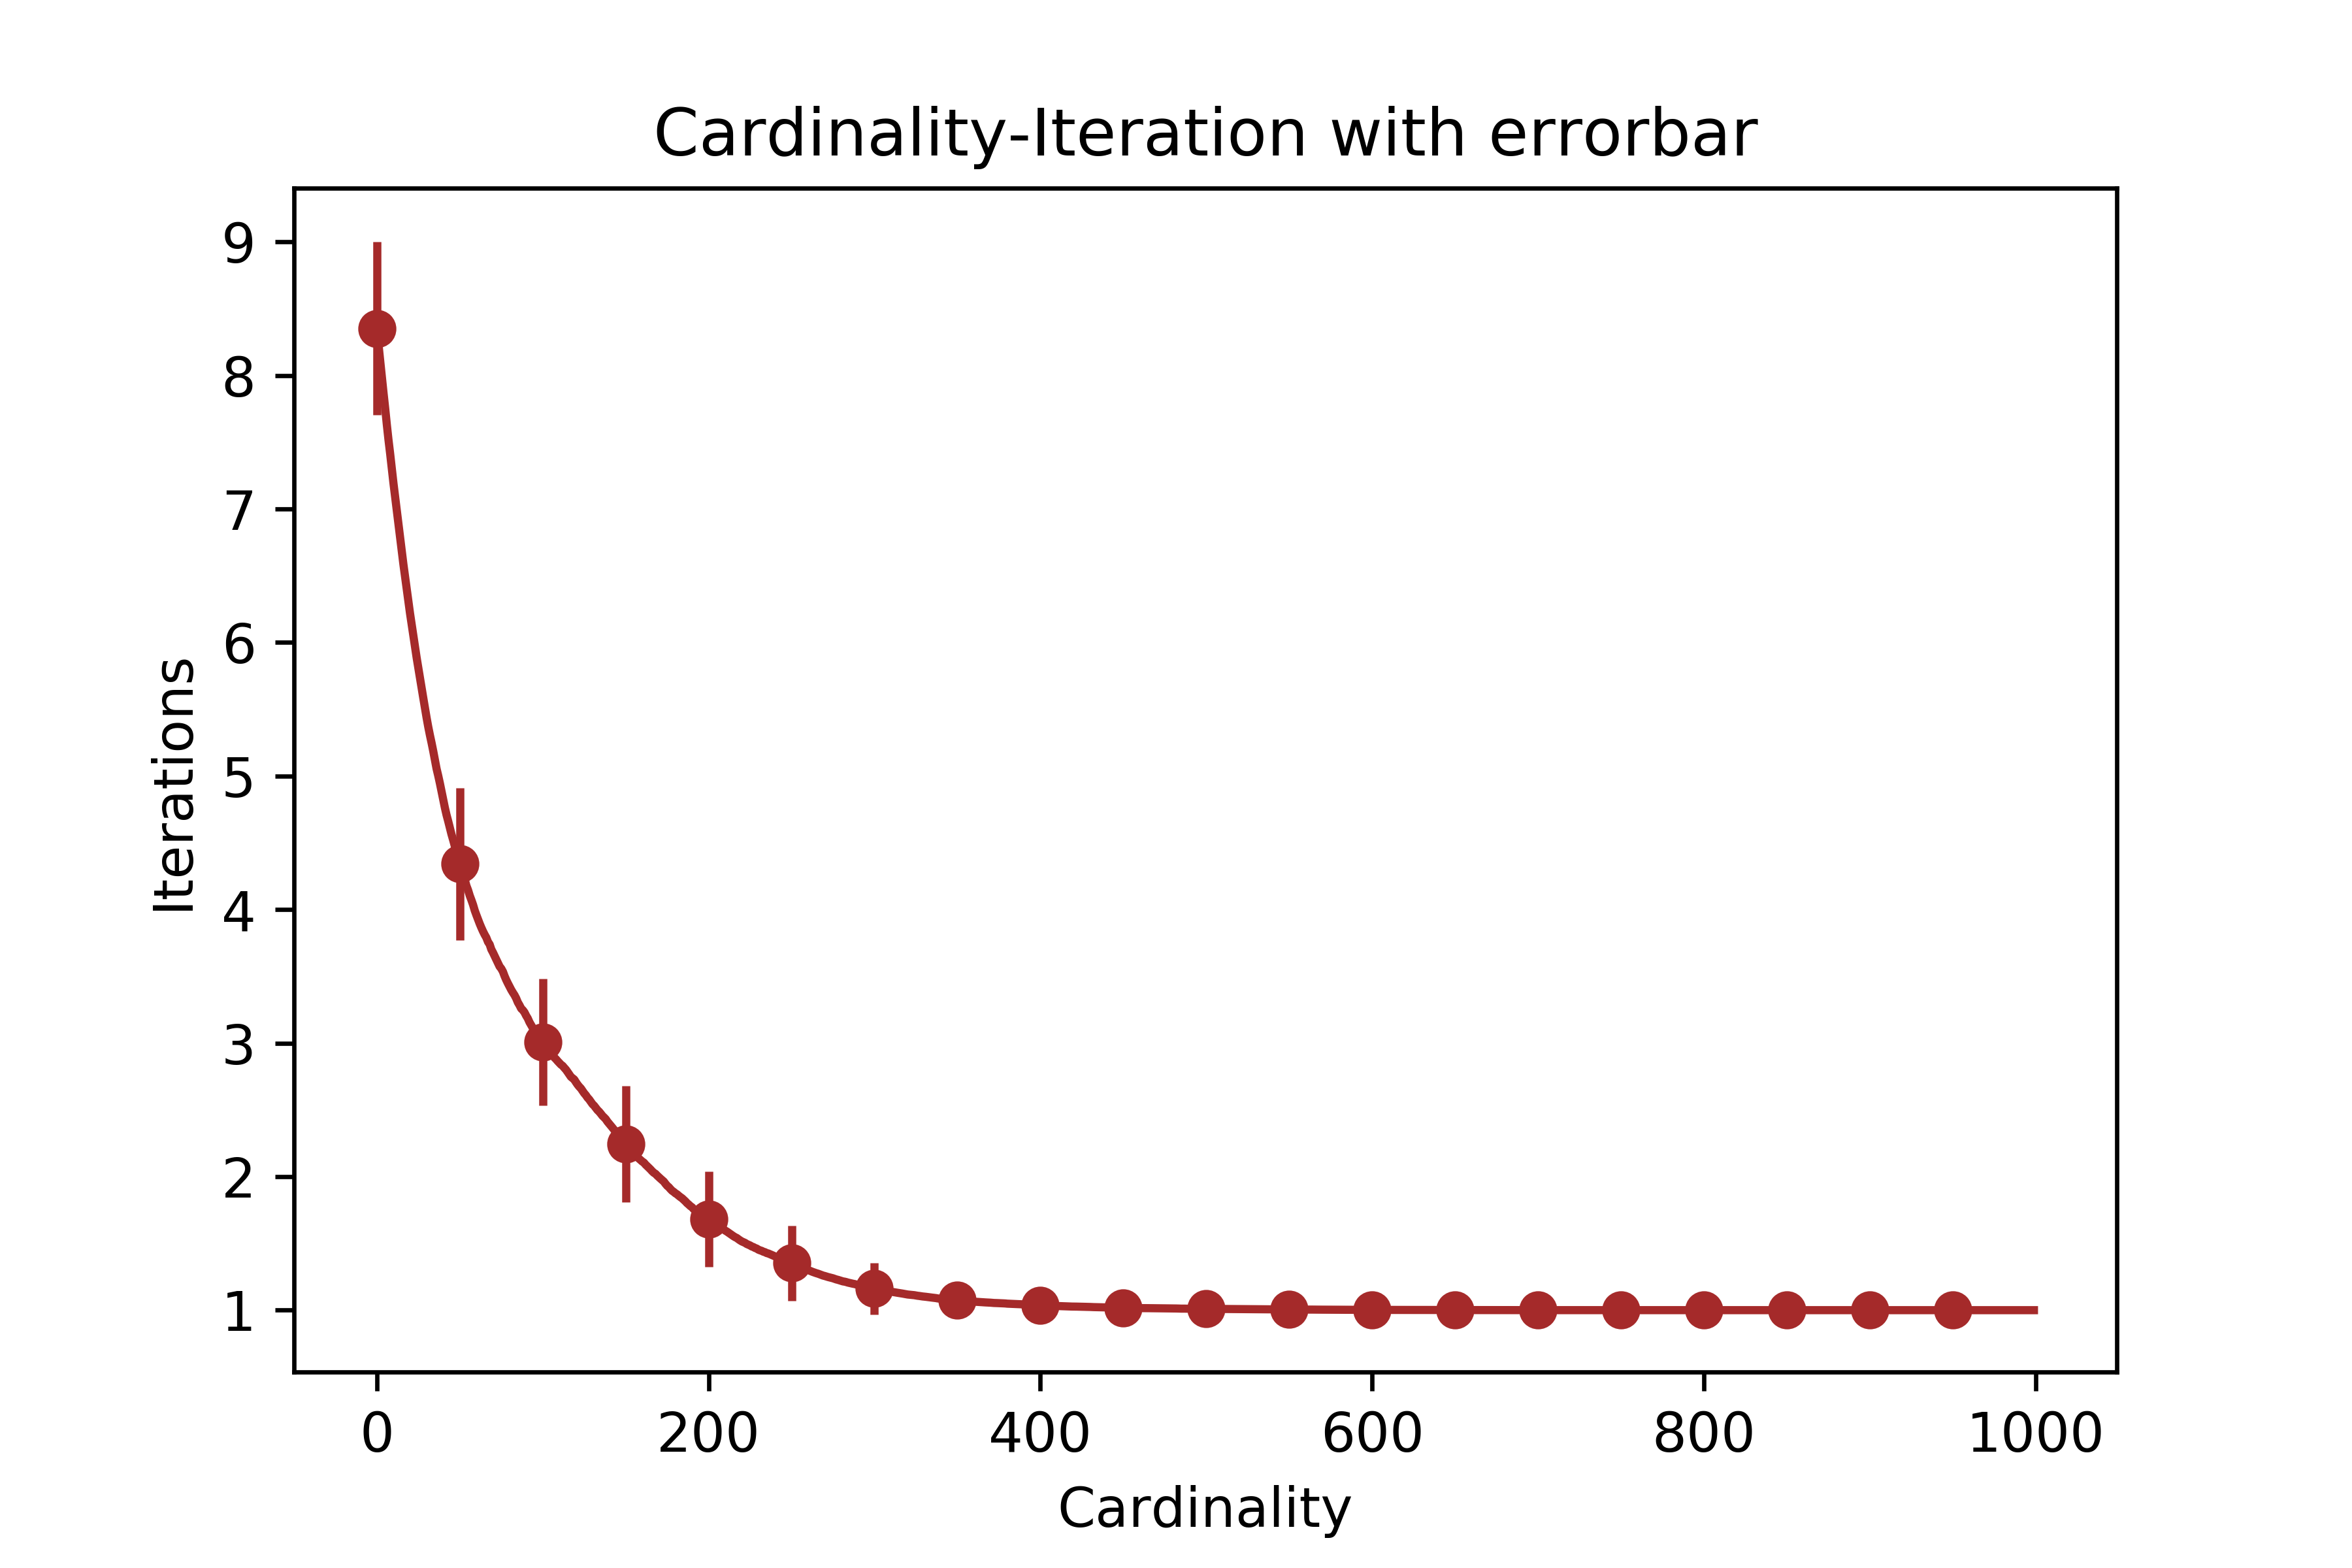
\includegraphics[width=0.9\textwidth]{CardErr50_4_1000_800}
    	\caption{Cardinality with error bar}\label{CardErr50_4_1000_800}
    \end{figure}
    \subsection{50\_4\_1000\_800}
    \subsubsection*{Experiment~1}
    Time used: 1423.639460532976
    \begin{figure}[H]
    	\centering
    	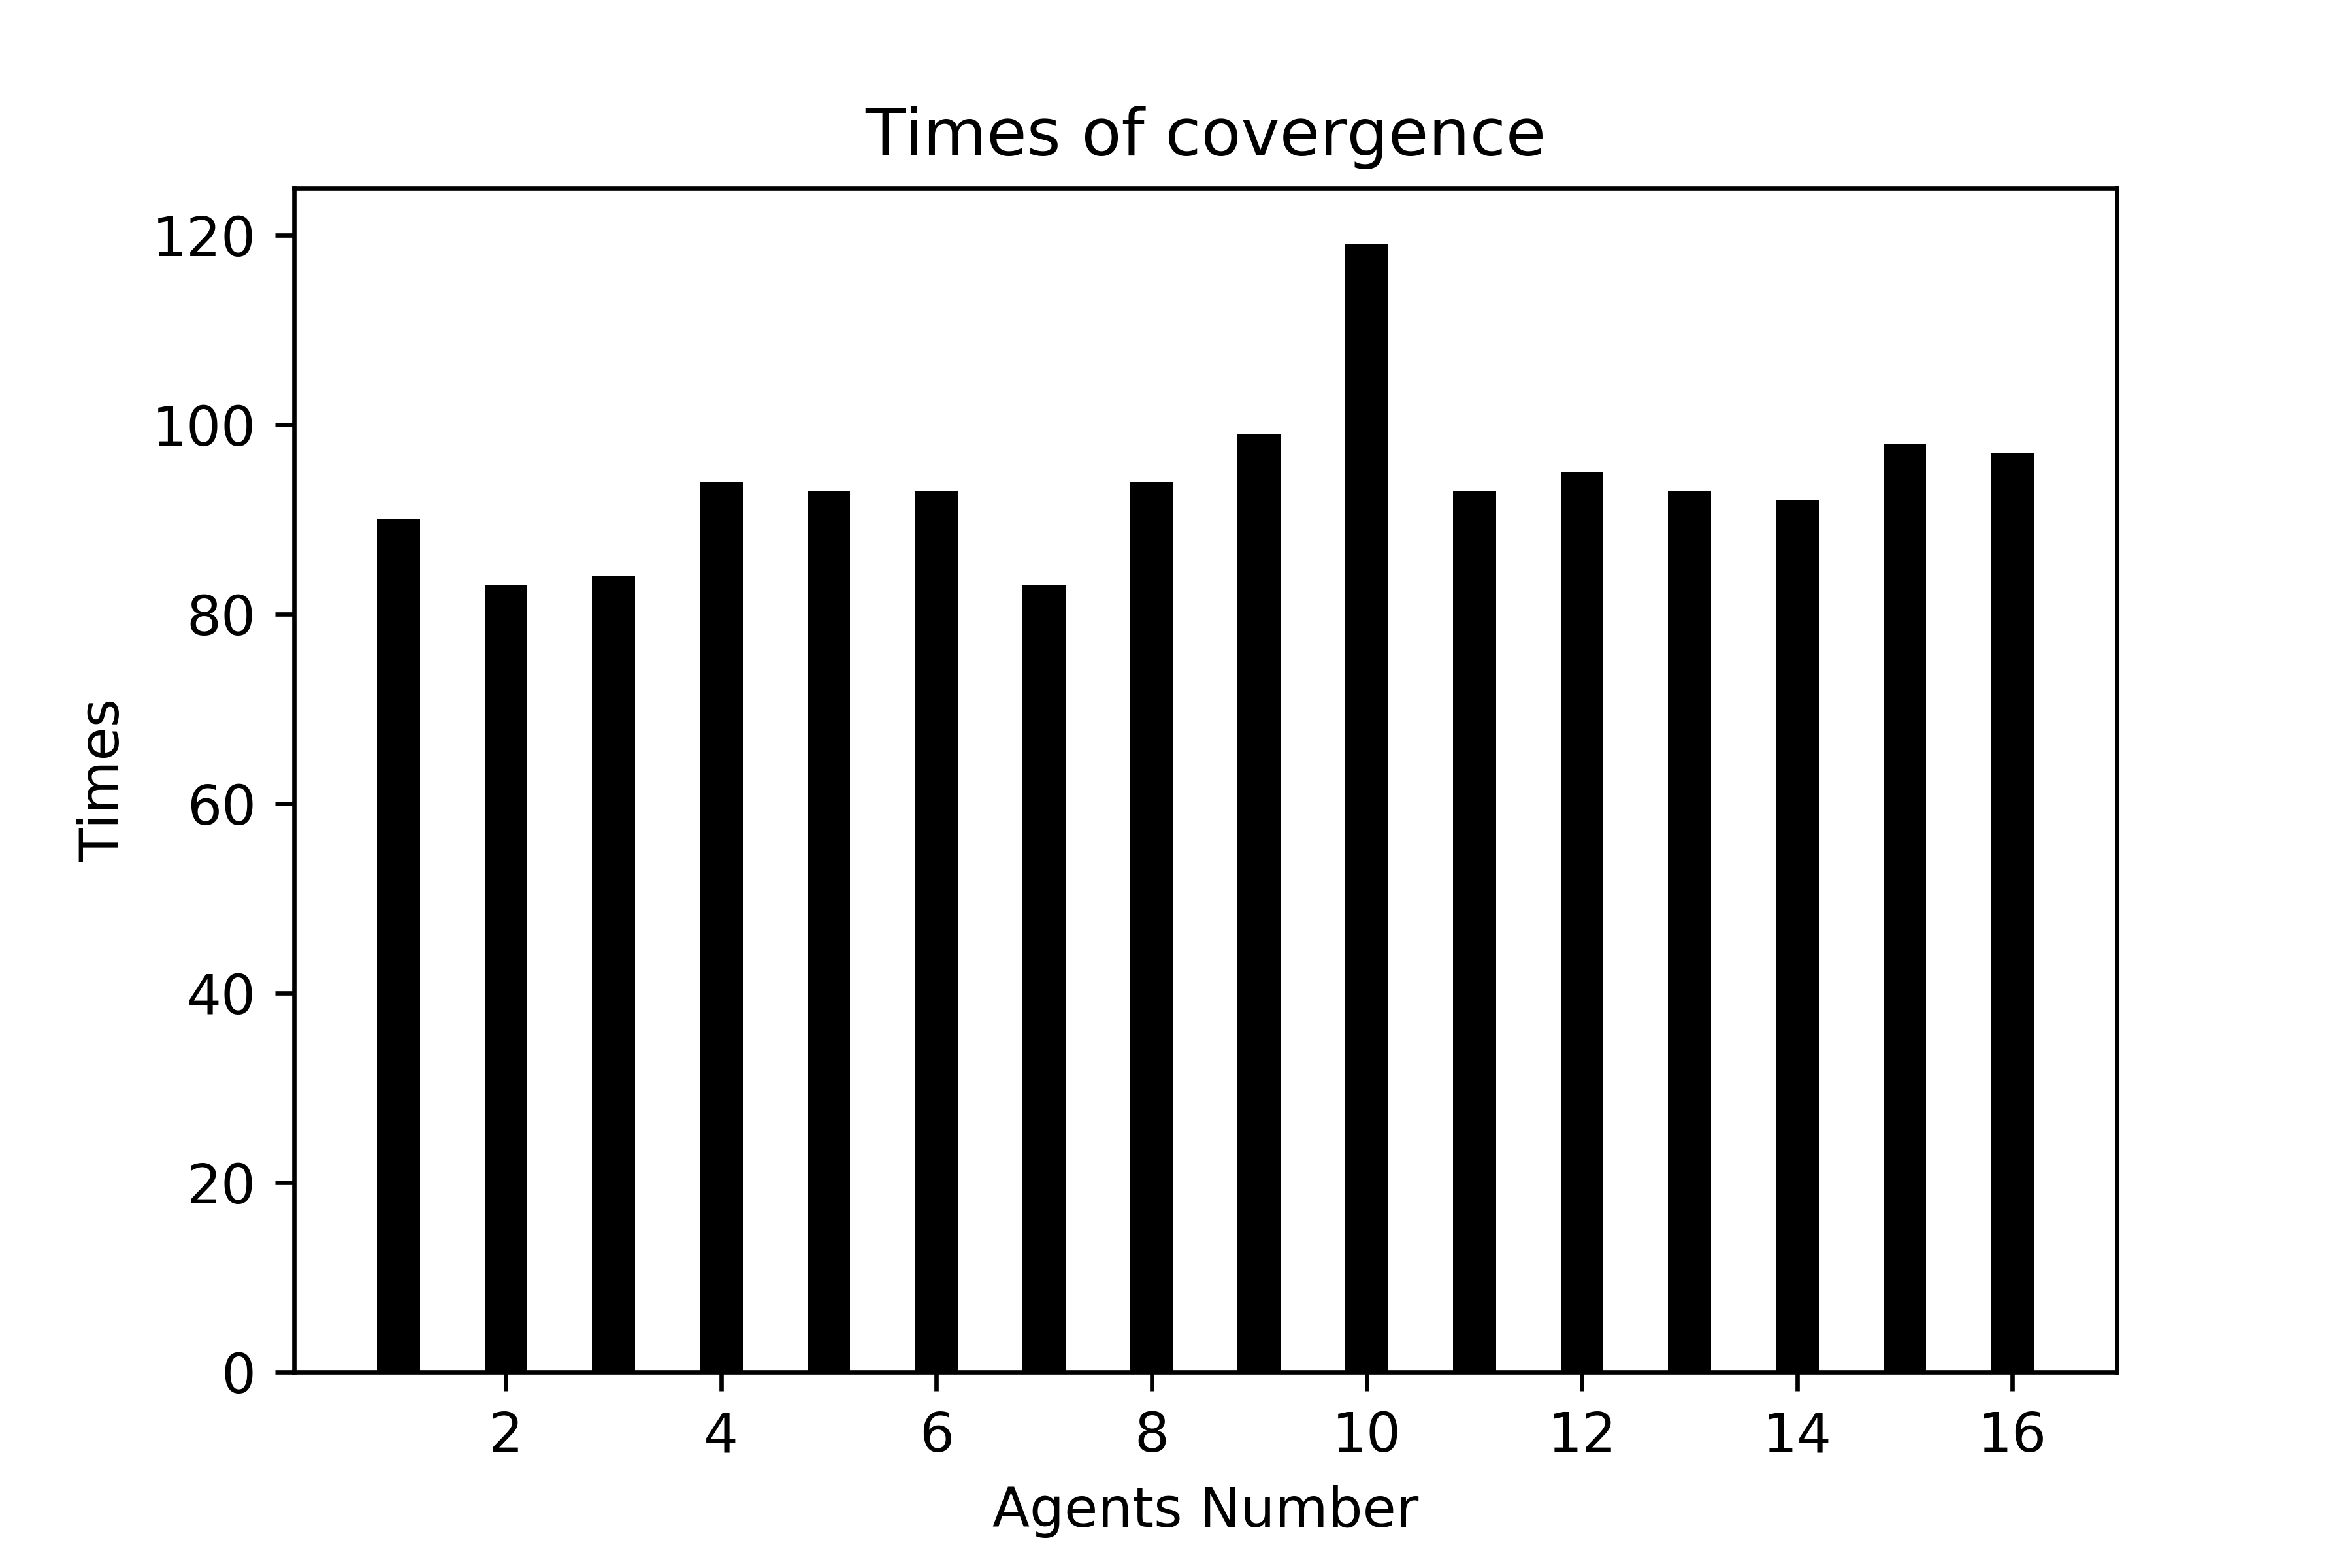
\includegraphics[width=0.9\textwidth]{agt50_4_1000_1500}
    	\caption{Where the iterations converge}\label{agt50_4_1000_1500}
    \end{figure}
    %
    \begin{figure}[H]
    	\centering
    	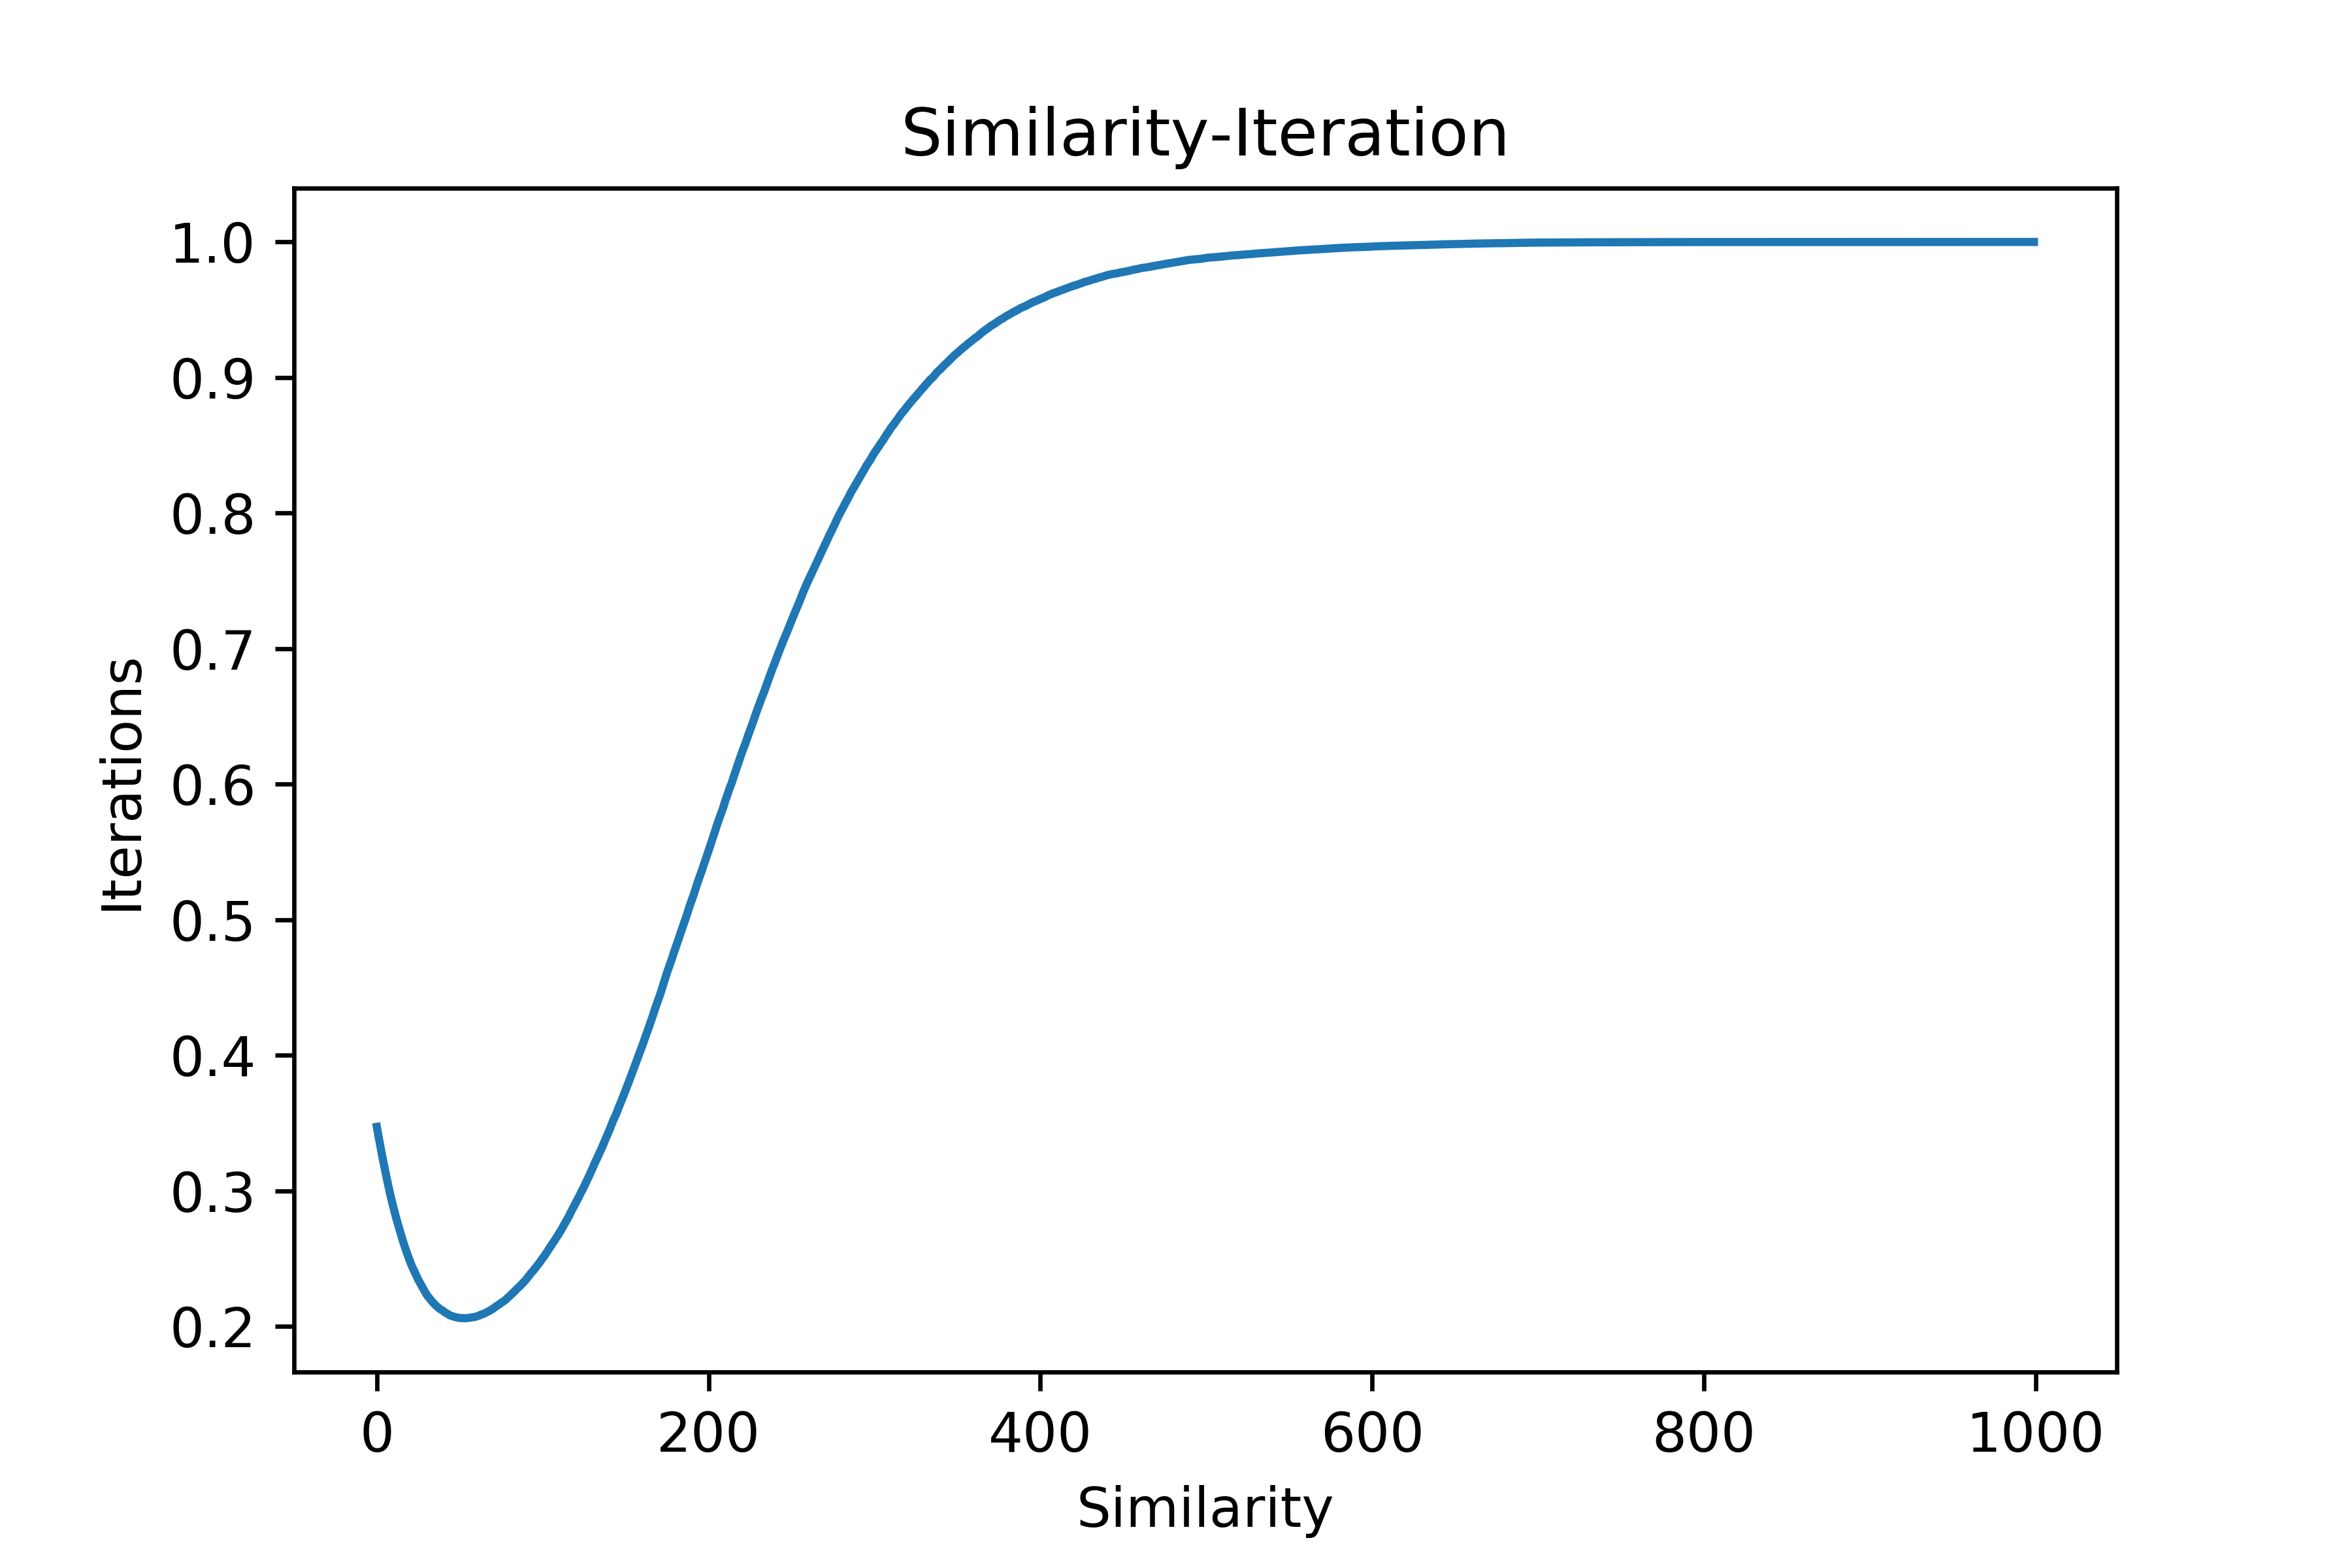
\includegraphics[width=0.9\textwidth]{Sim50_4_1000_1500}
    	\caption{Similarity}\label{Sim50_4_1000_1500}
    \end{figure}
    %
    \begin{figure}[H]
    	\centering
    	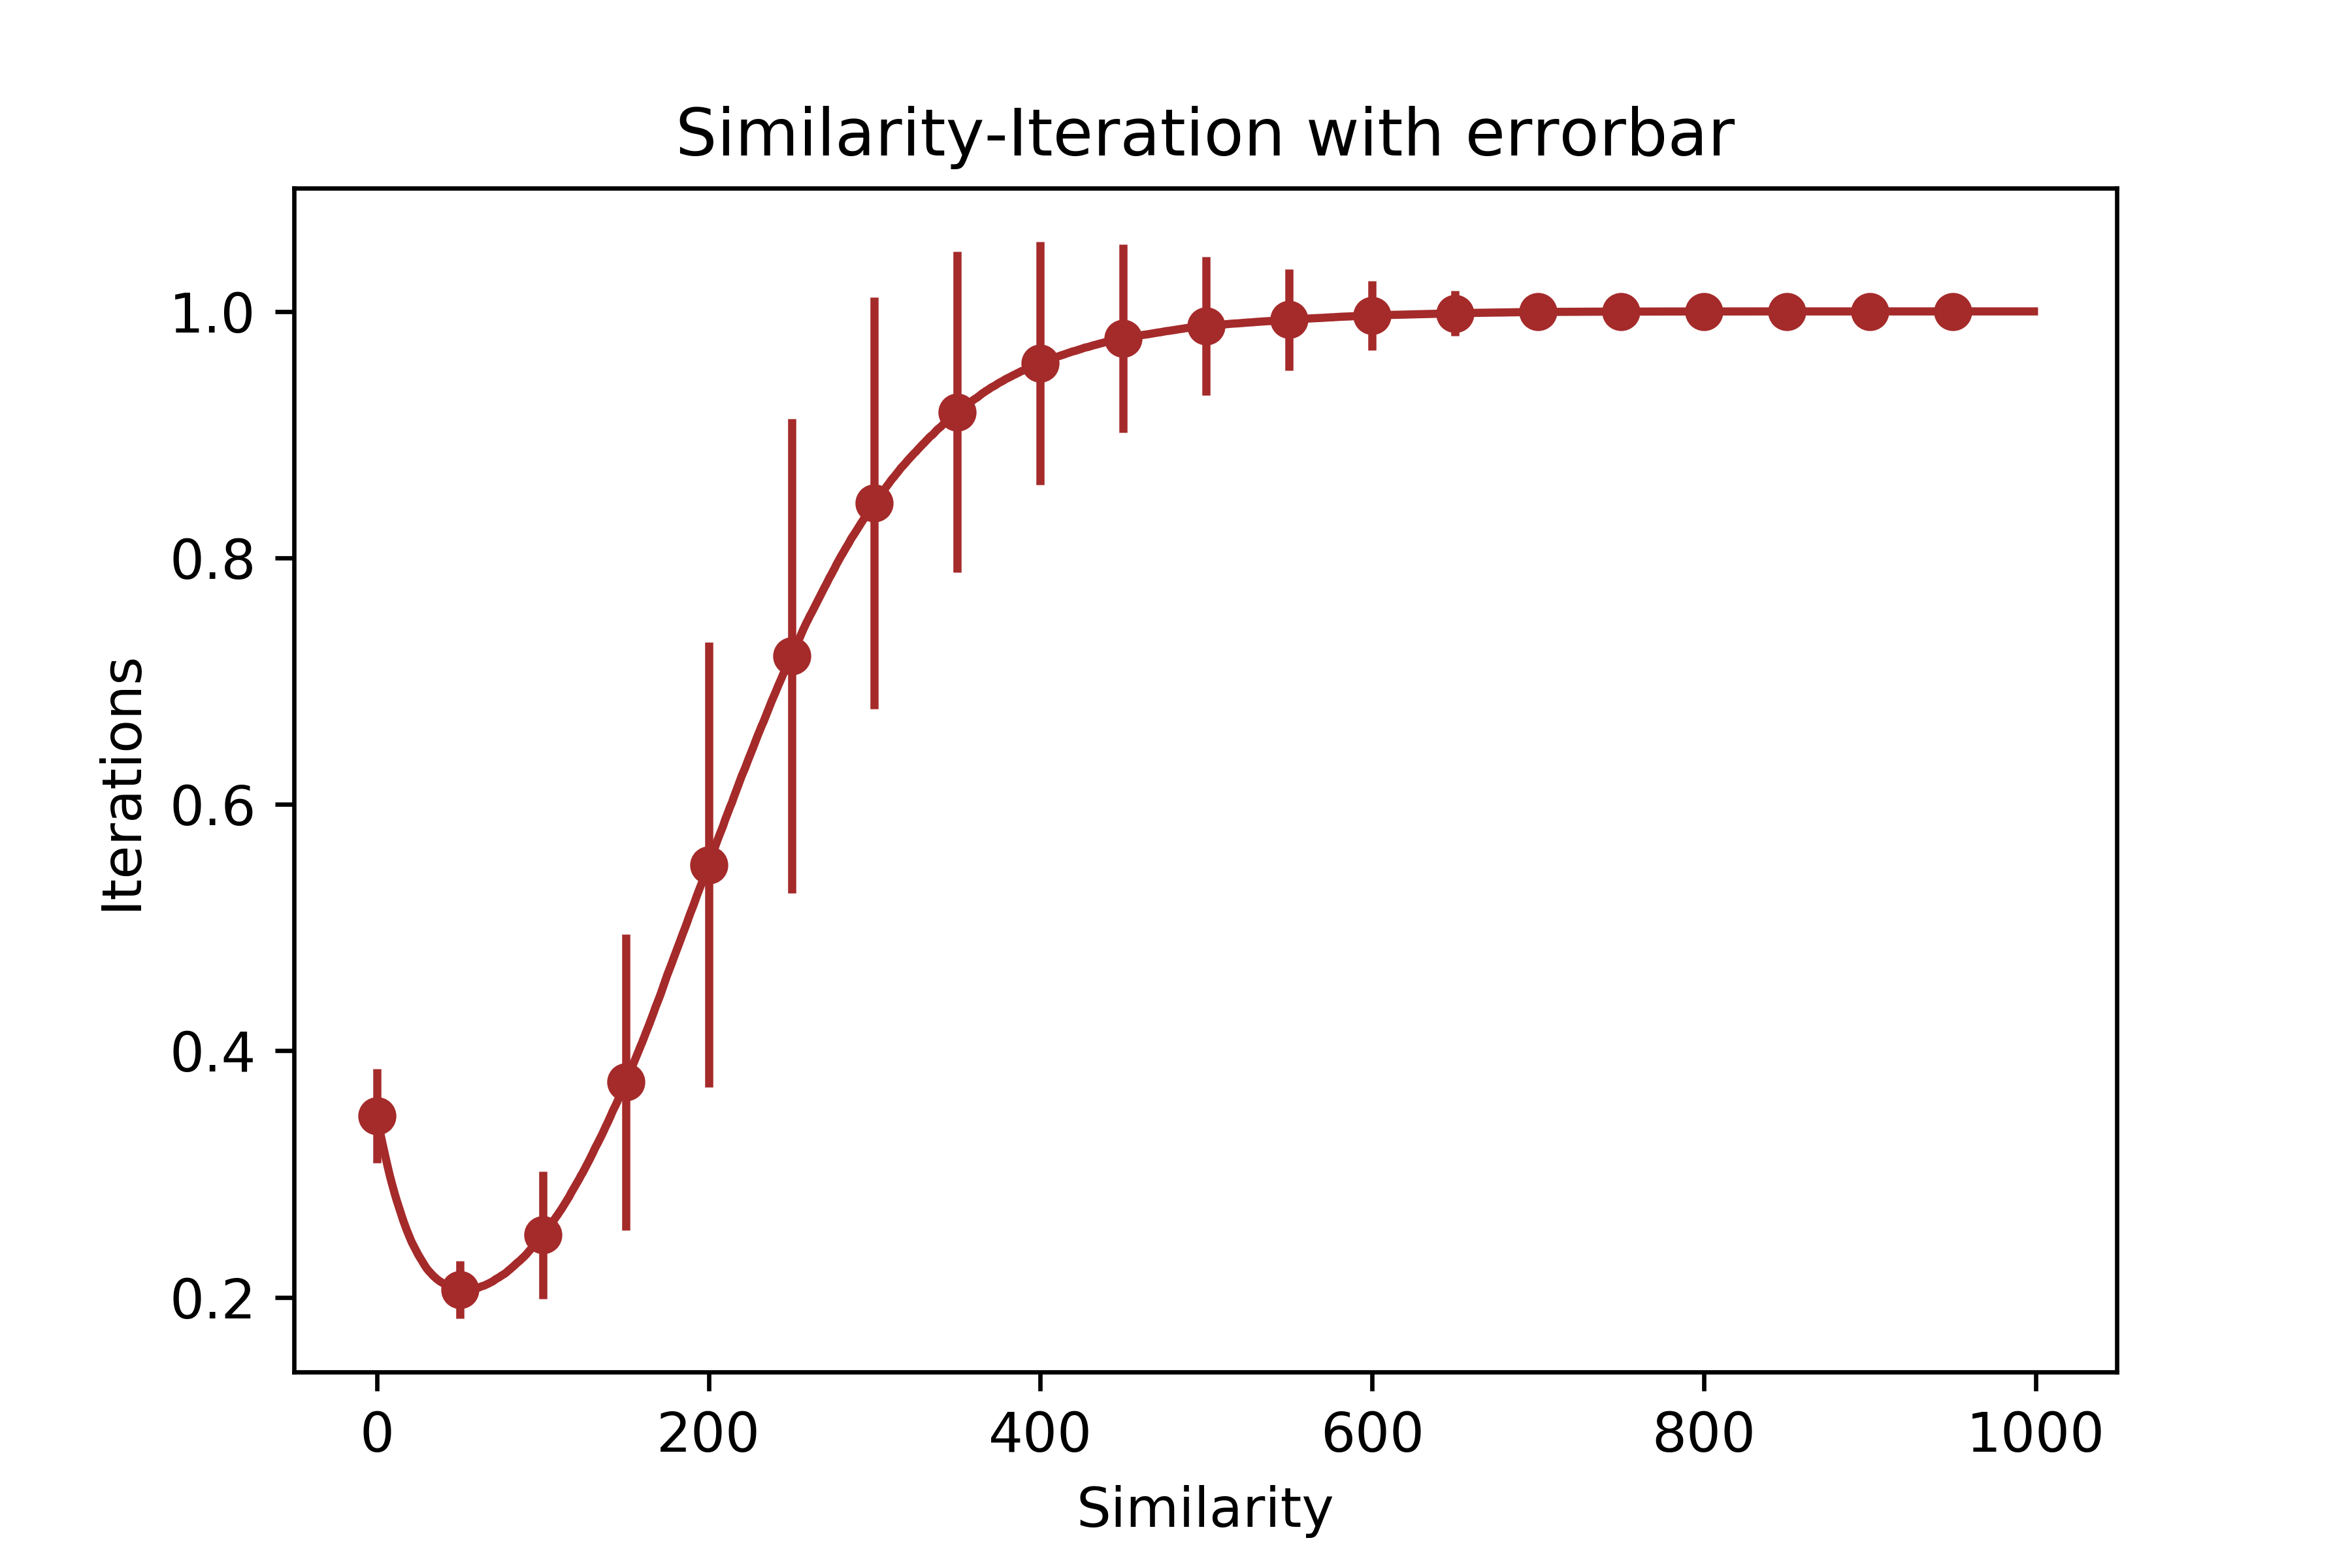
\includegraphics[width=0.9\textwidth]{SimErr50_4_1000_1500}
    	\caption{Similarity with error bar}\label{SimErr50_4_1000_1500}
    \end{figure}
    %
    \begin{figure}[H]
    	\centering
    	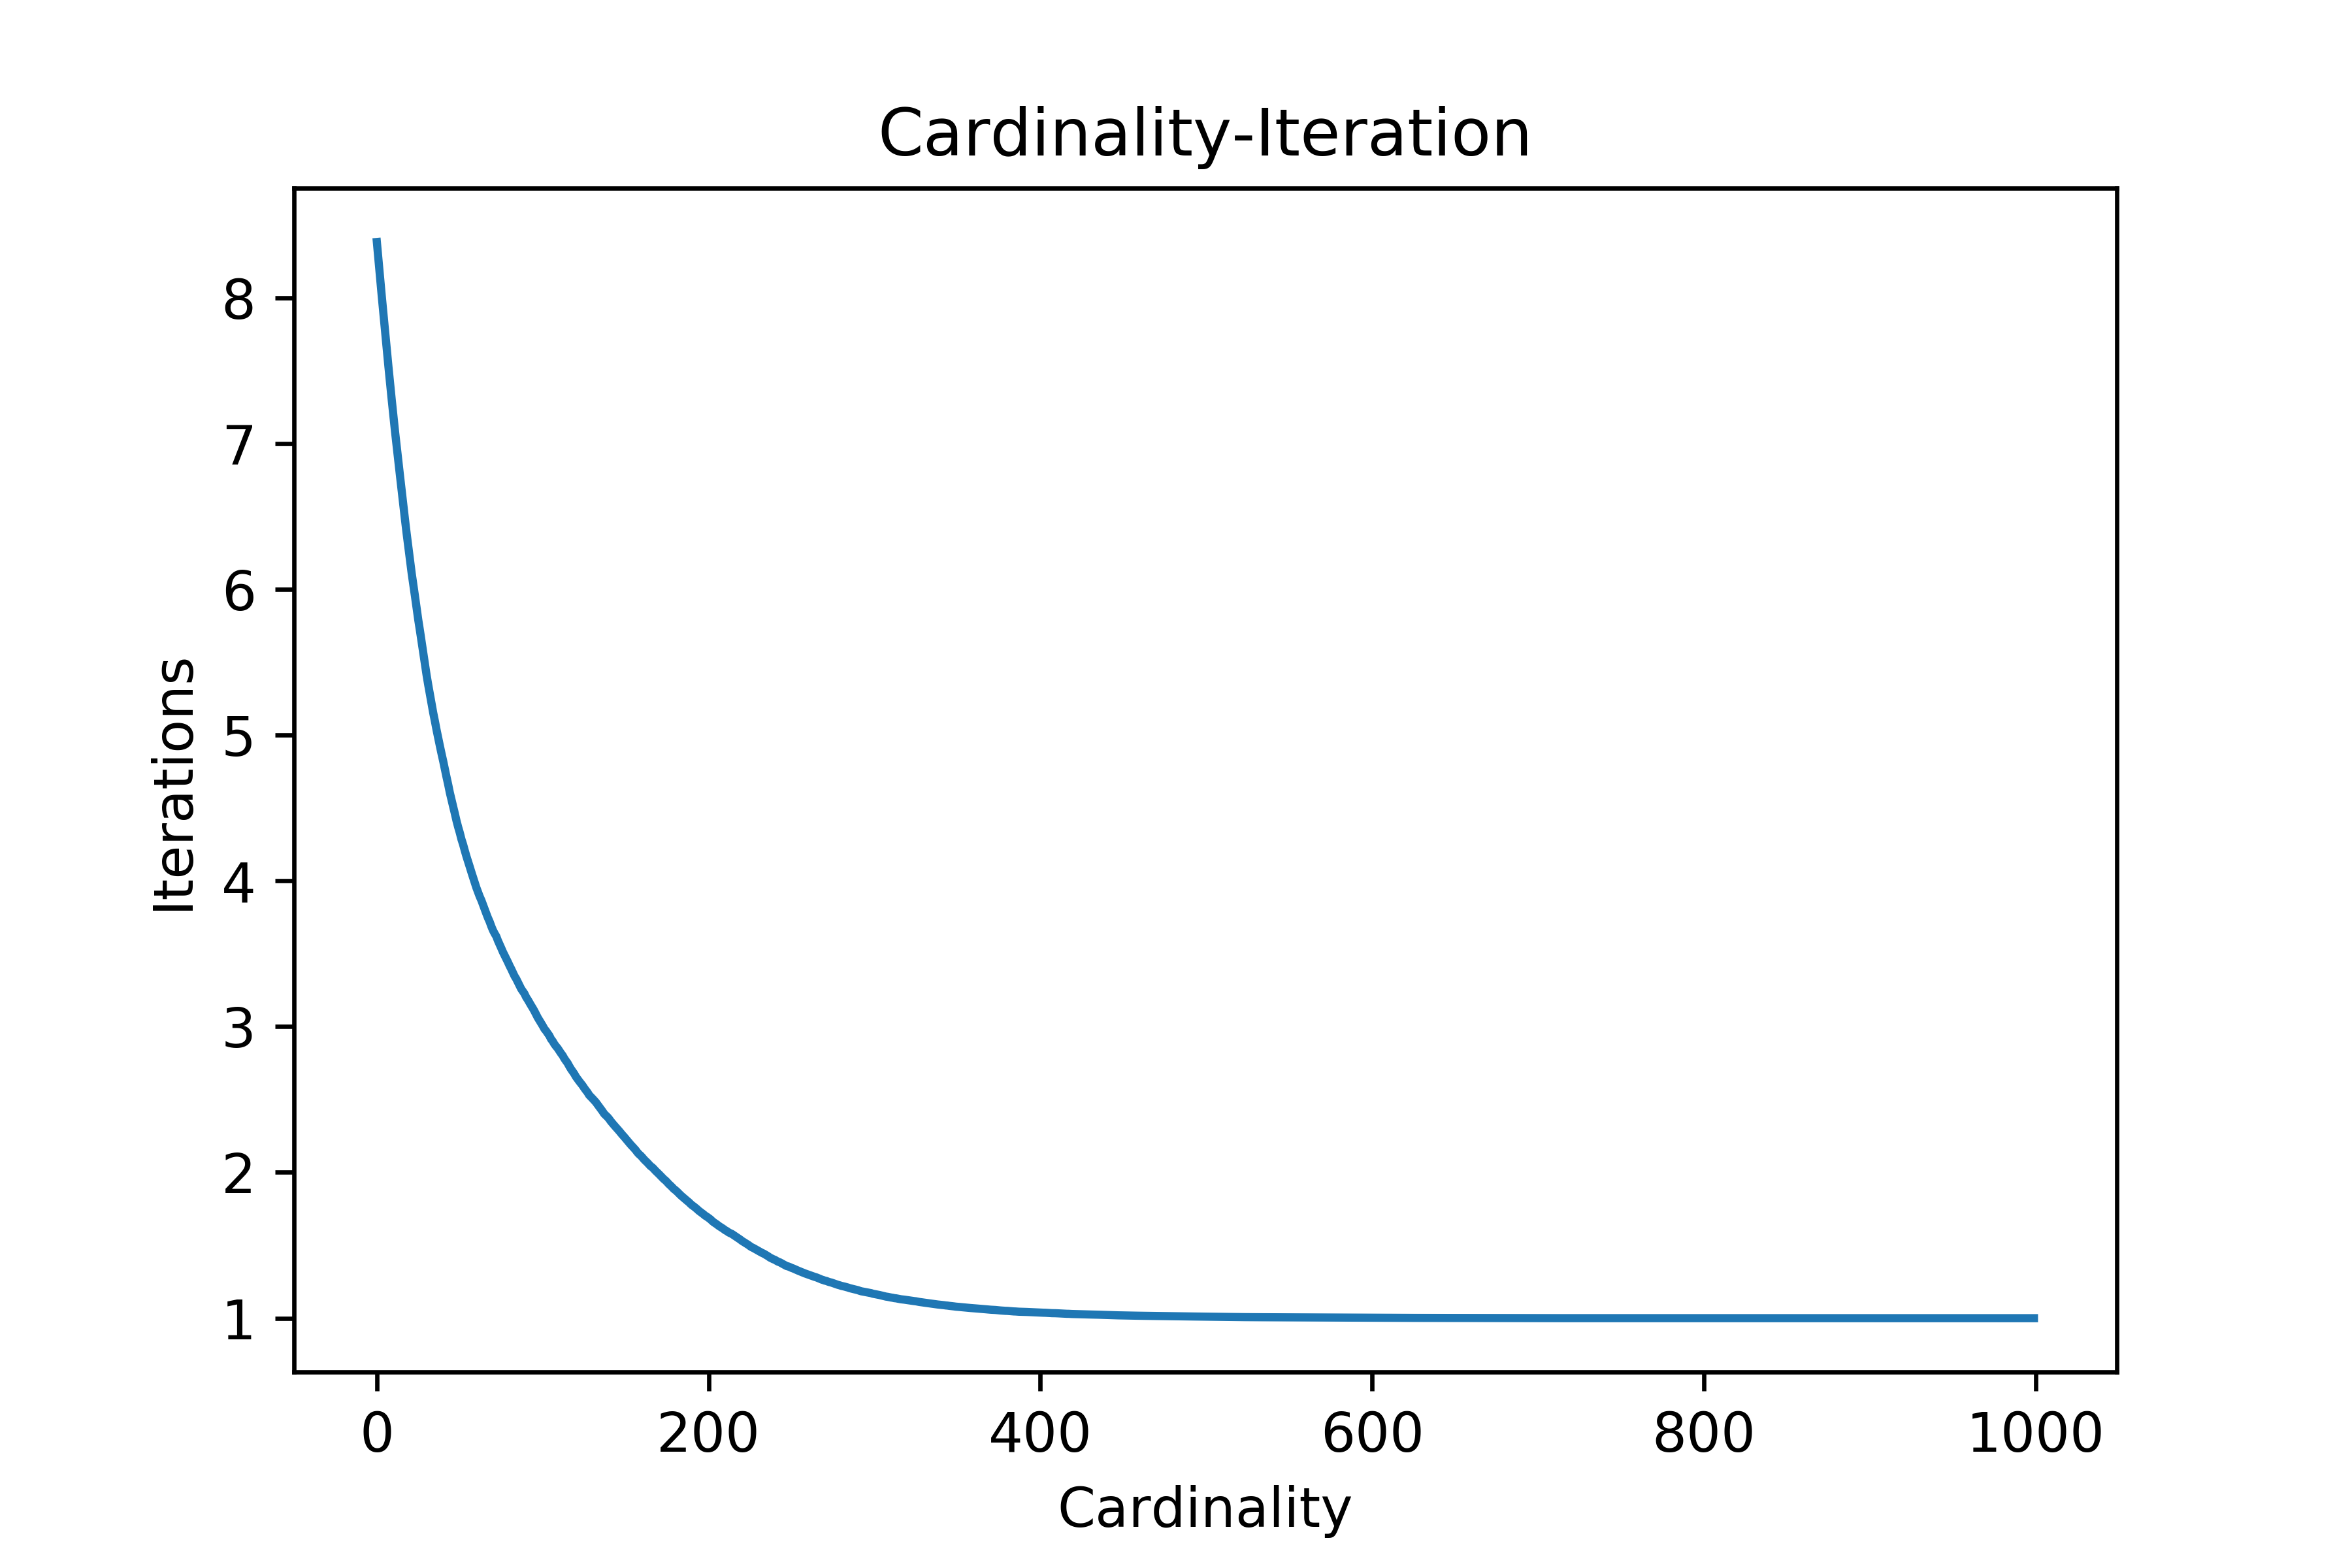
\includegraphics[width=0.9\textwidth]{Card50_4_1000_1500}
    	\caption{Cardinality}\label{Card50_4_1000_1500}
    \end{figure}
    %
    \begin{figure}[H]
    	\centering
    	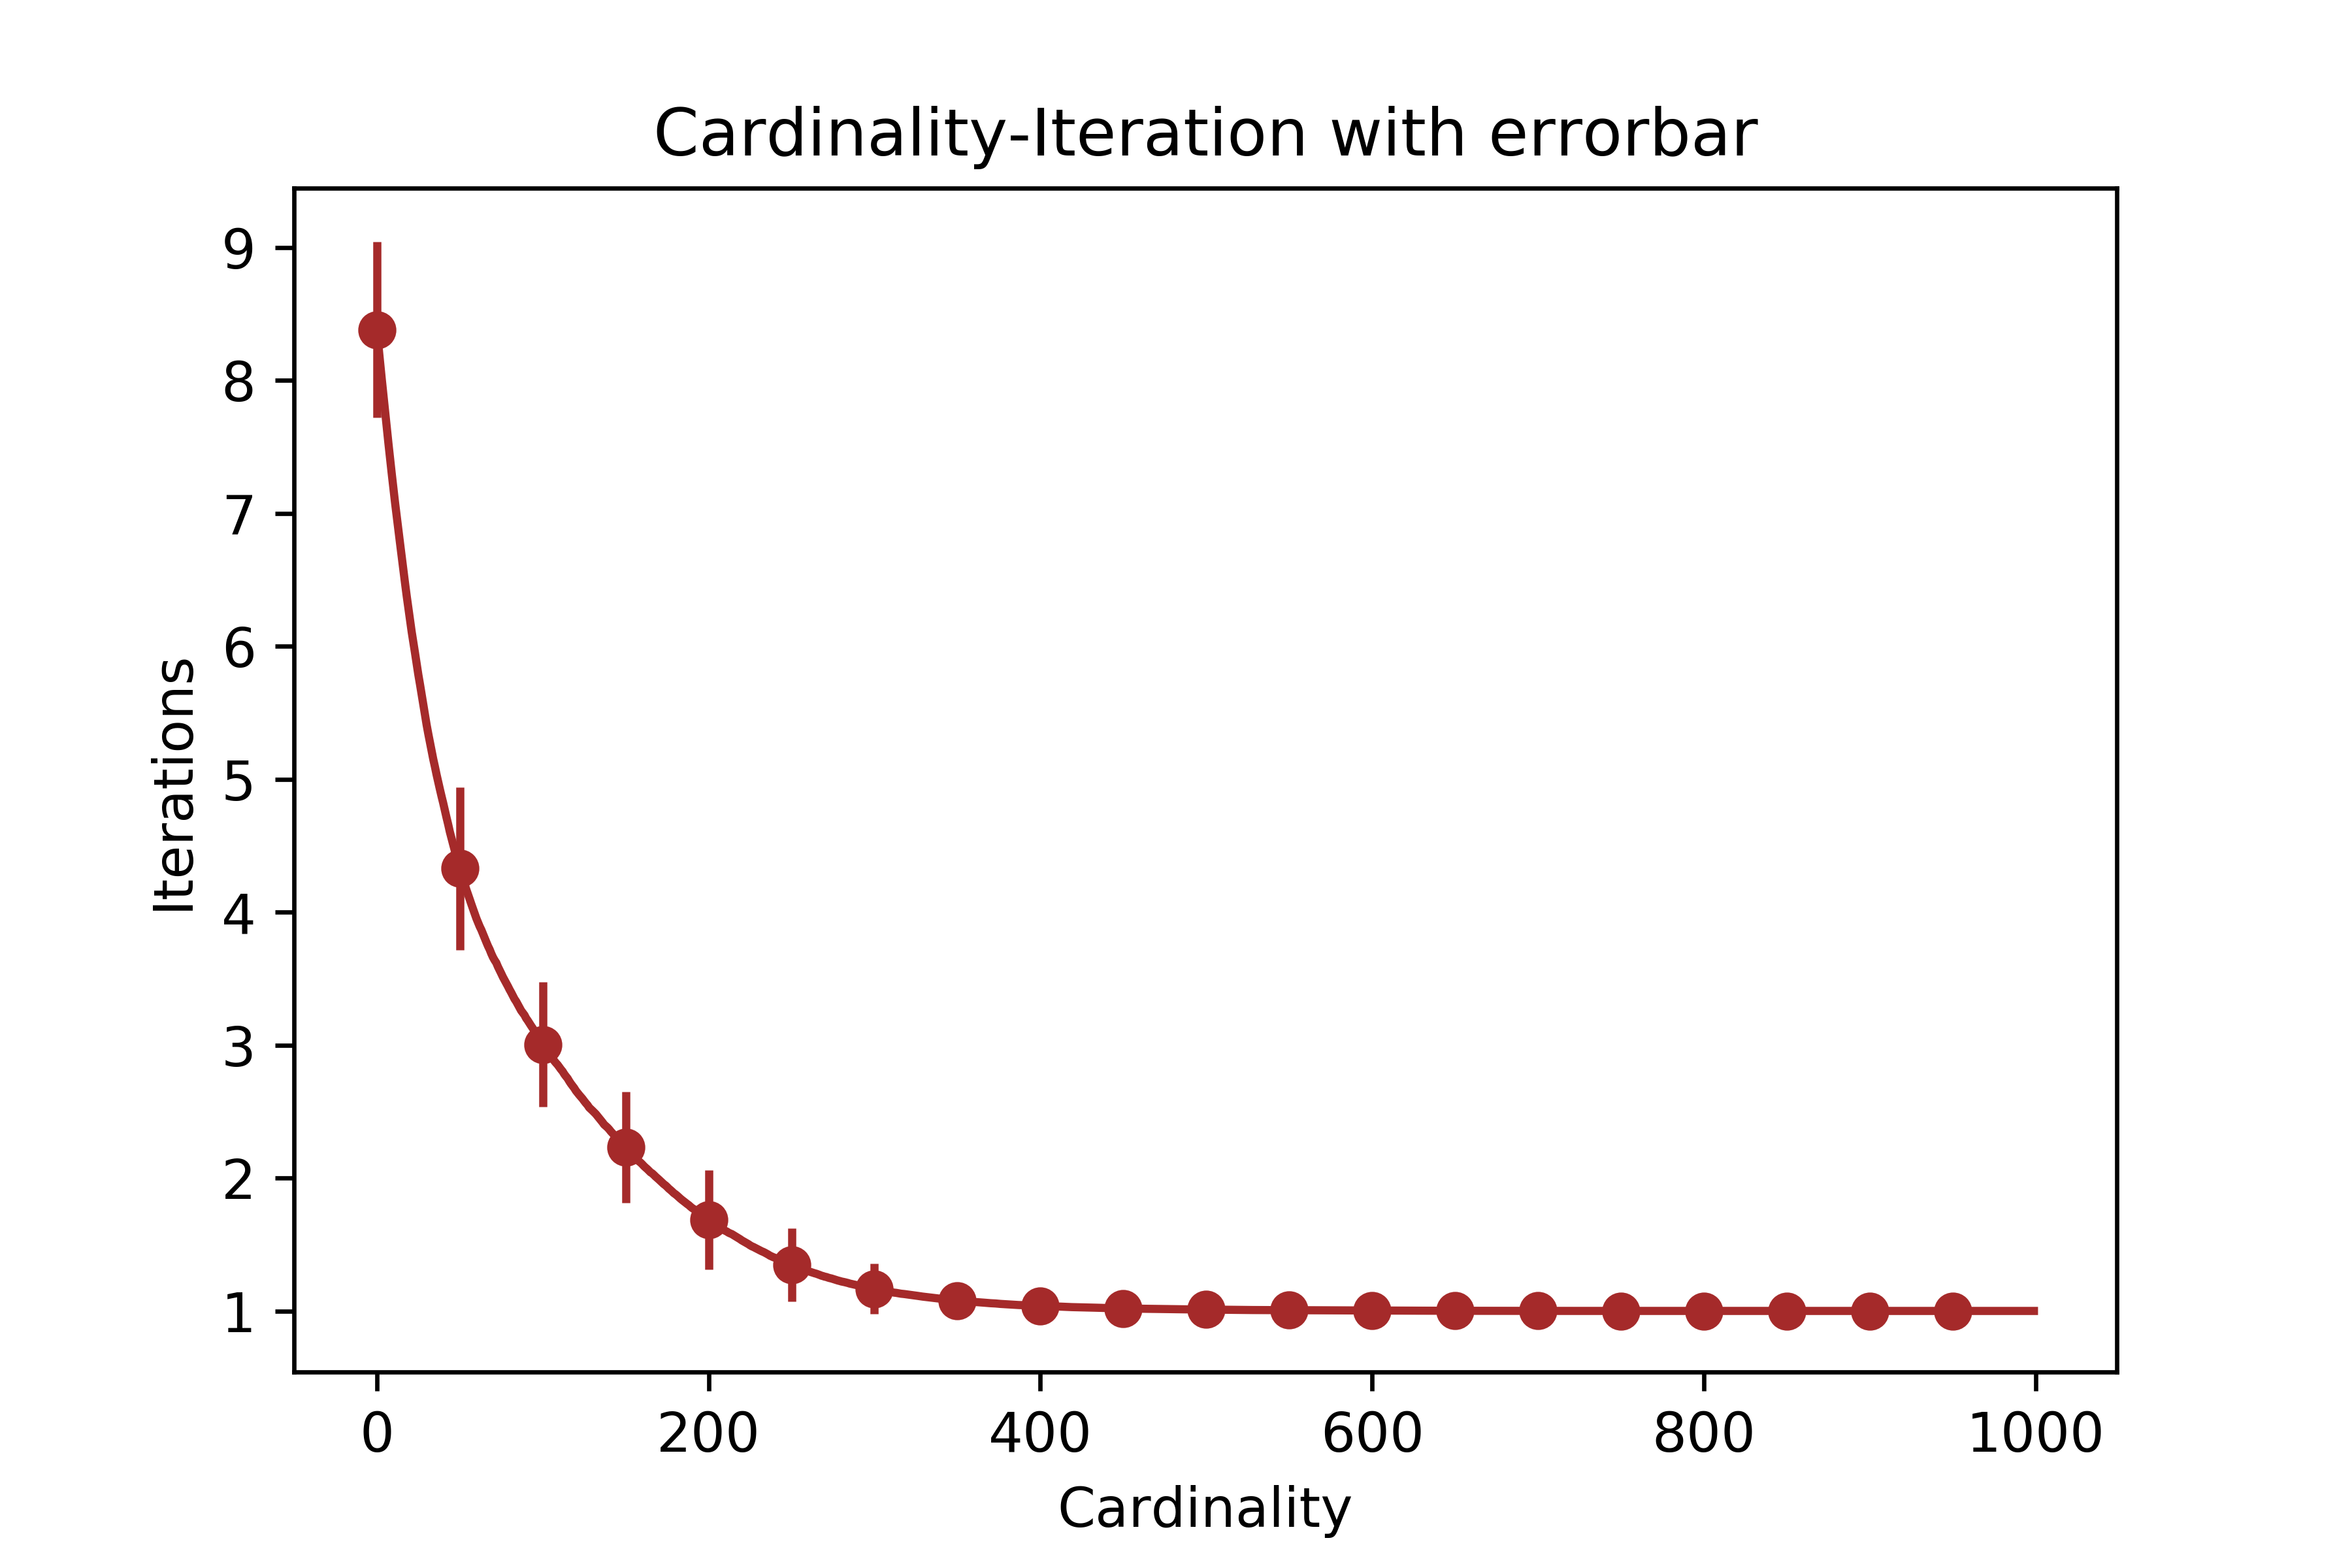
\includegraphics[width=0.9\textwidth]{CardErr50_4_1000_1500}
    	\caption{Cardinality with error bar}\label{CardErr50_4_1000_1500}
    \end{figure}
    %
     \subsubsection*{Experiment~2}
     Time used: 2714.9842374045834(too long due the sleep of computer)
    \begin{figure}[H]
    	\centering
    	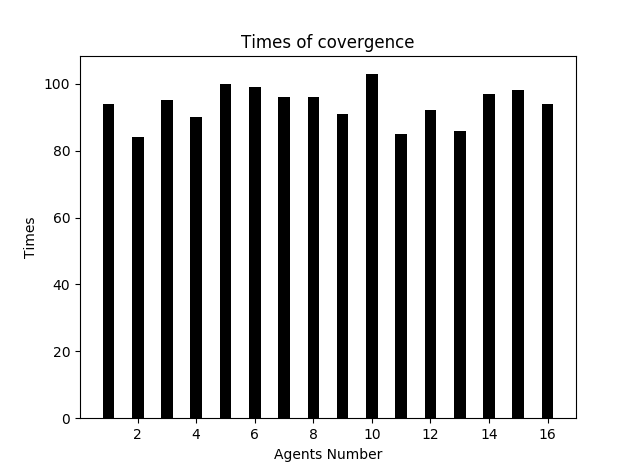
\includegraphics[width=0.9\textwidth]{agt50_4_1000_1500_e2}
    	\caption{Where the iterations converge}\label{agt50_4_1000_1500_e2}
    \end{figure}
    %
    \begin{figure}[H]
    	\centering
    	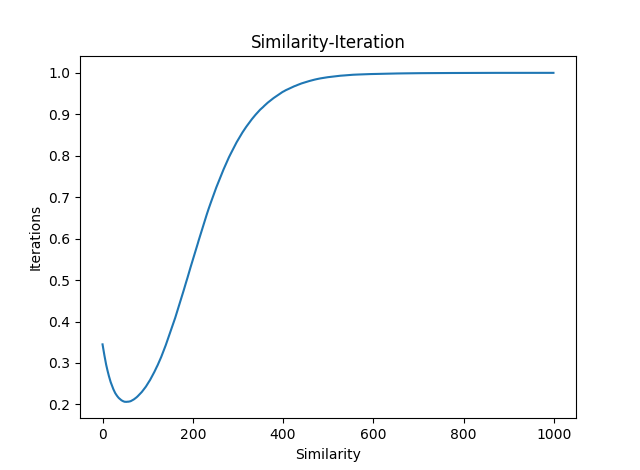
\includegraphics[width=0.9\textwidth]{Sim50_4_1000_1500_e2}
    	\caption{Similarity}\label{Sim50_4_1000_1500_e2}
    \end{figure}
    %
    \begin{figure}[H]
    	\centering
    	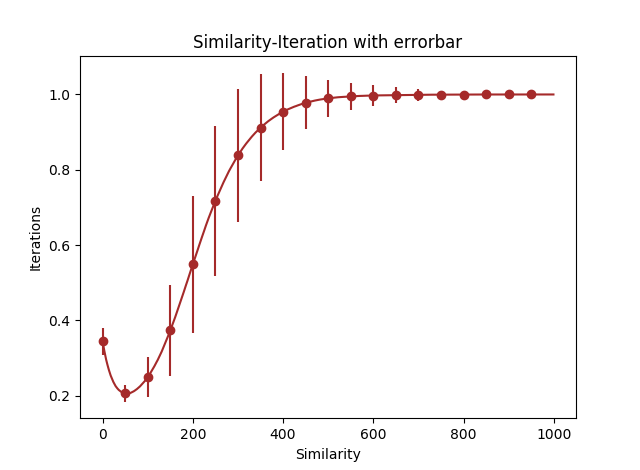
\includegraphics[width=0.9\textwidth]{SimErr50_4_1000_1500_e2}
    	\caption{Similarity with error bar}\label{SimErr50_4_1000_1500_e2}
    \end{figure}
    %
    \begin{figure}[H]
    	\centering
    	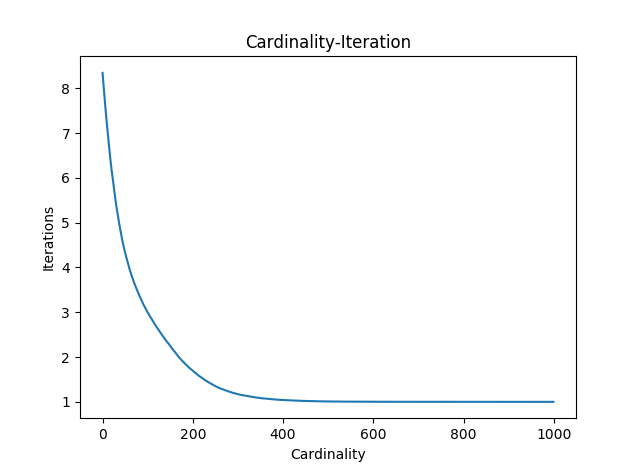
\includegraphics[width=0.9\textwidth]{Card50_4_1000_1500_e2}
    	\caption{Cardinality}\label{Card50_4_1000_1500_e2}
    \end{figure}
    %
    \begin{figure}[H]
    	\centering
    	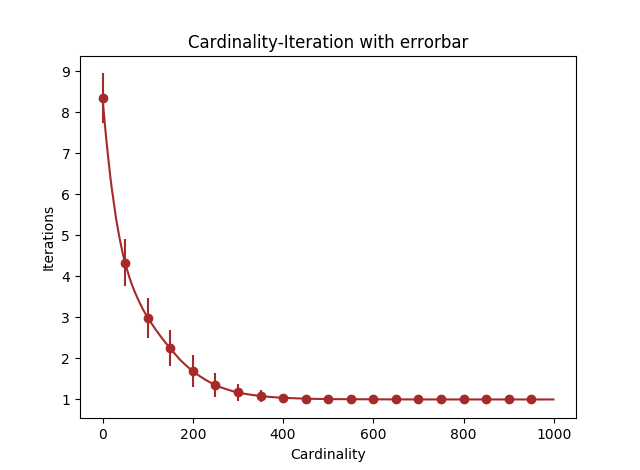
\includegraphics[width=0.9\textwidth]{CardErr50_4_1000_1500_e2}
    	\caption{Cardinality with error bar}\label{CardErr50_4_1000_1500_e2}
    \end{figure}
    %
    \subsubsection*{Experiment~3}
    Time used: 1232.8931827431234
    \begin{figure}[H]
    	\centering
    	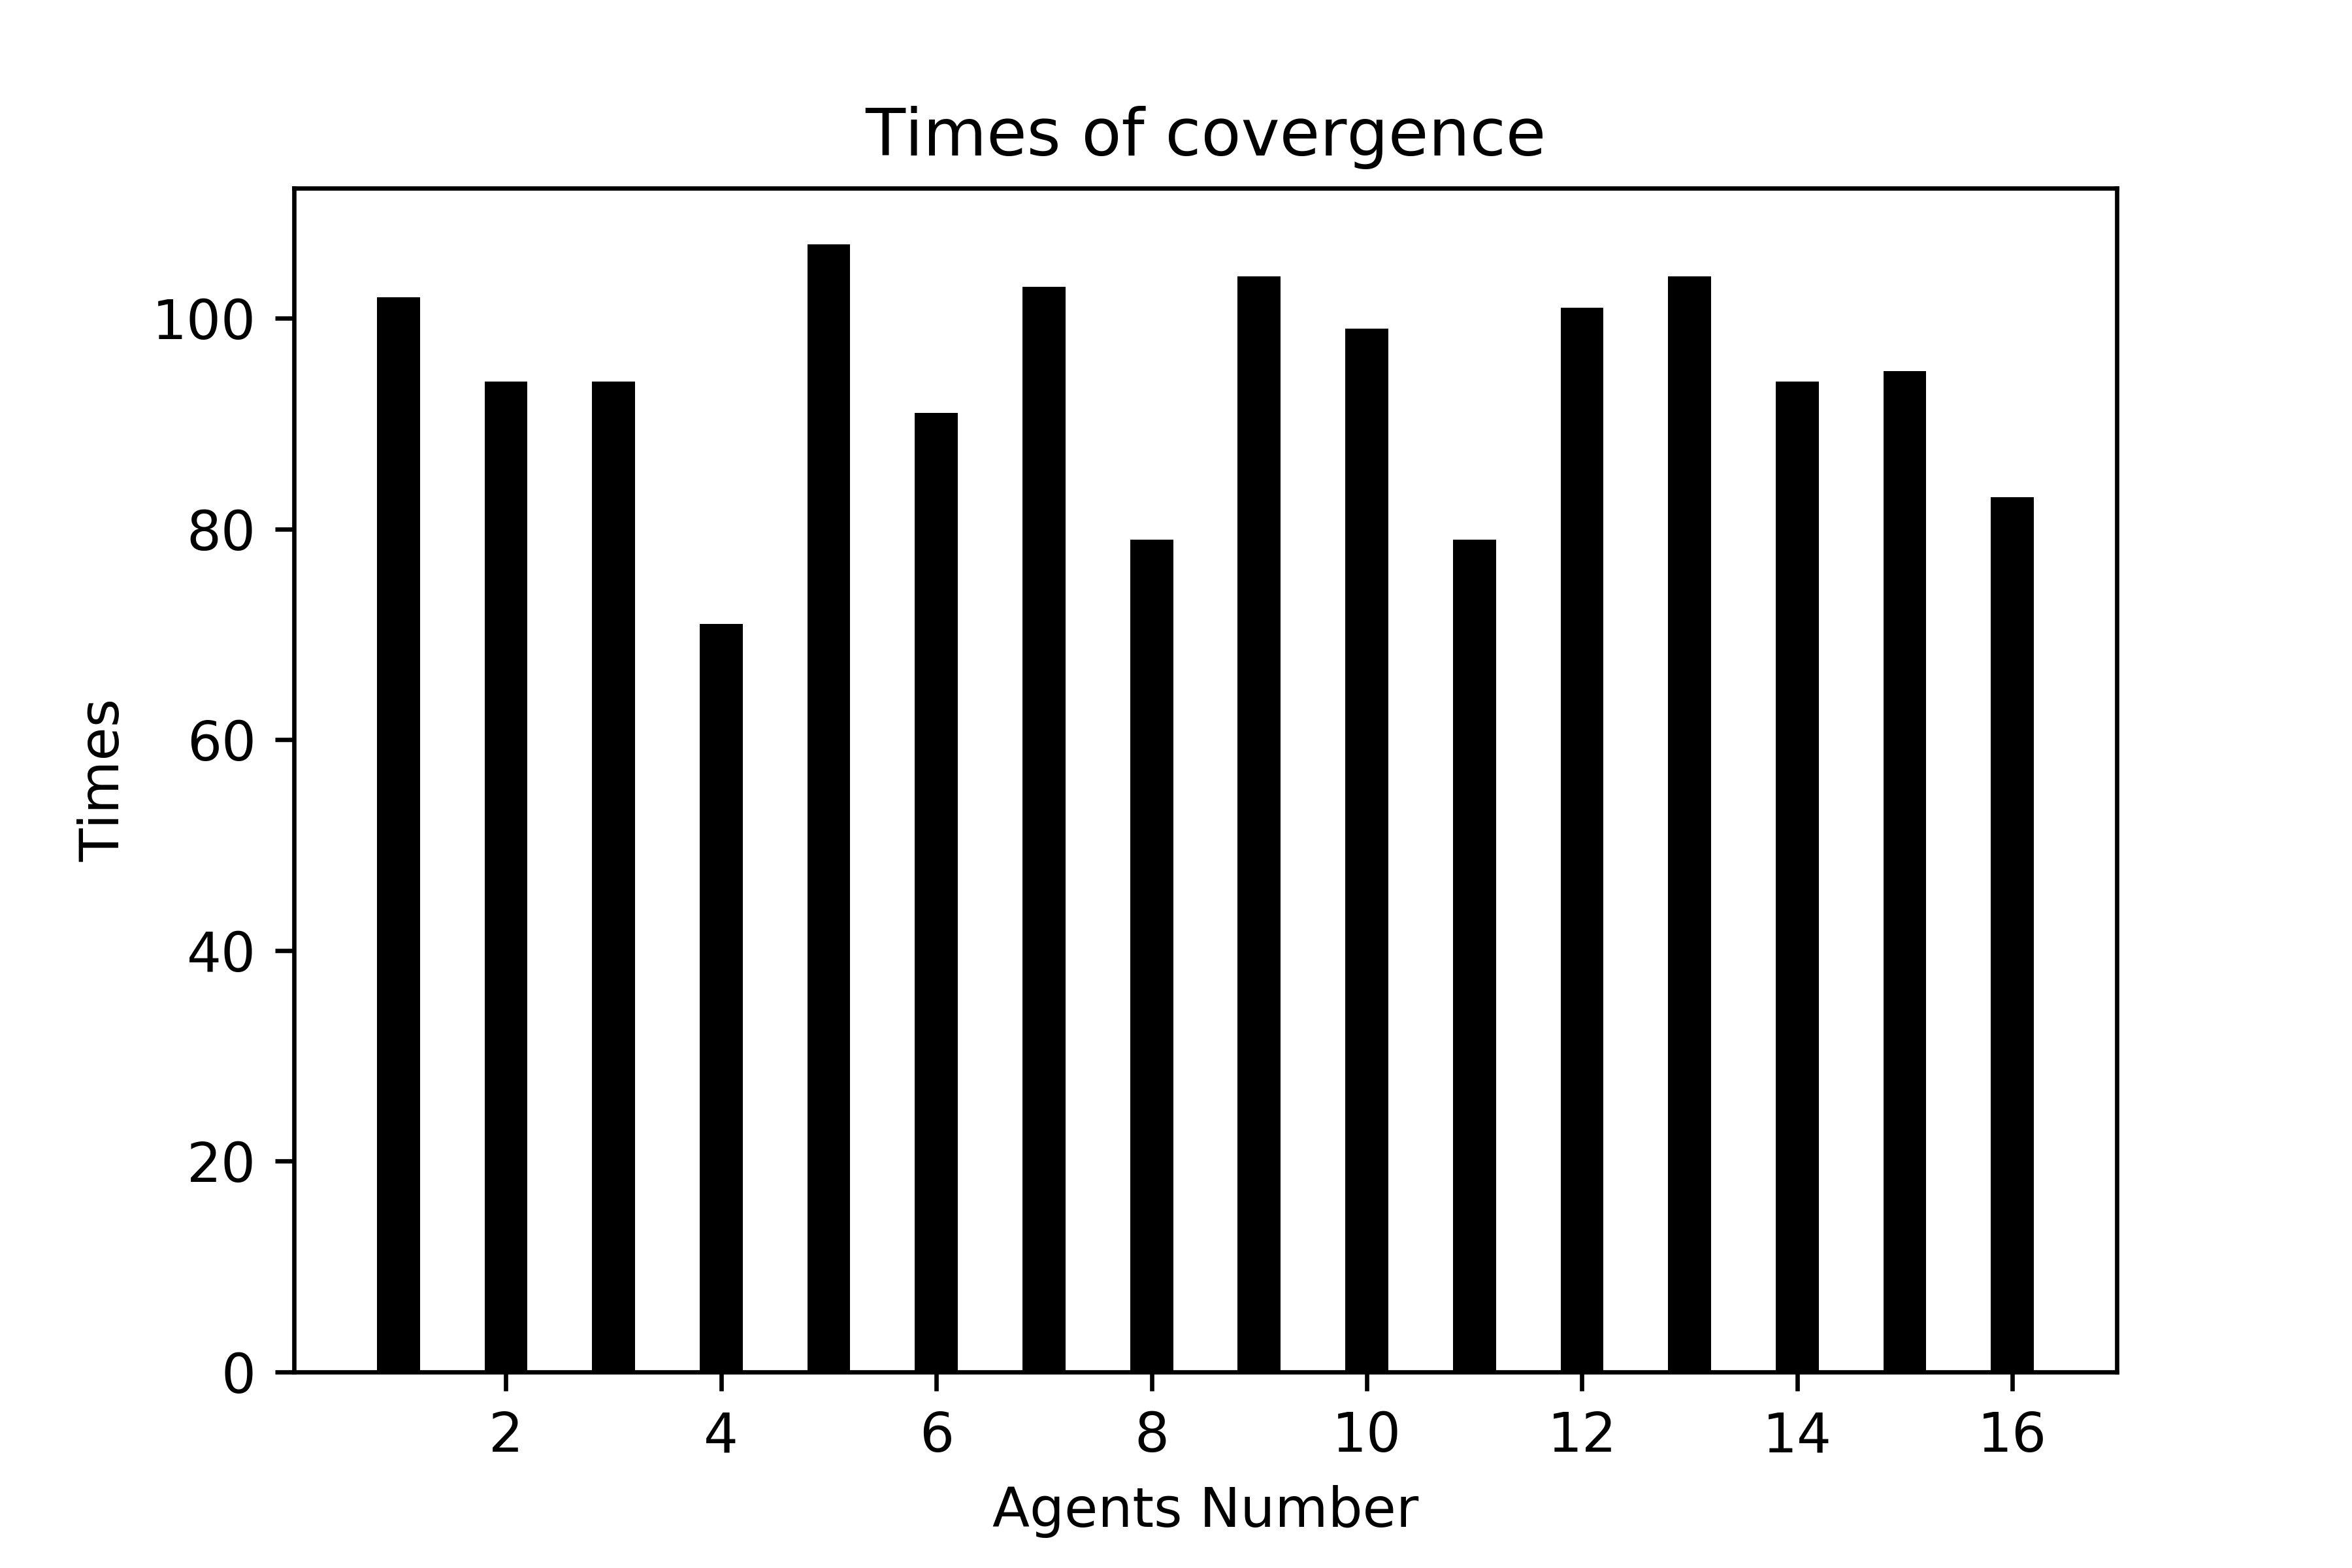
\includegraphics[width=0.9\textwidth]{agt50_4_1000_1500_e3}
    	\caption{Where the iterations converge}\label{agt50_4_1000_1500_e3}
    \end{figure}
    %
    \begin{figure}[H]
    	\centering
    	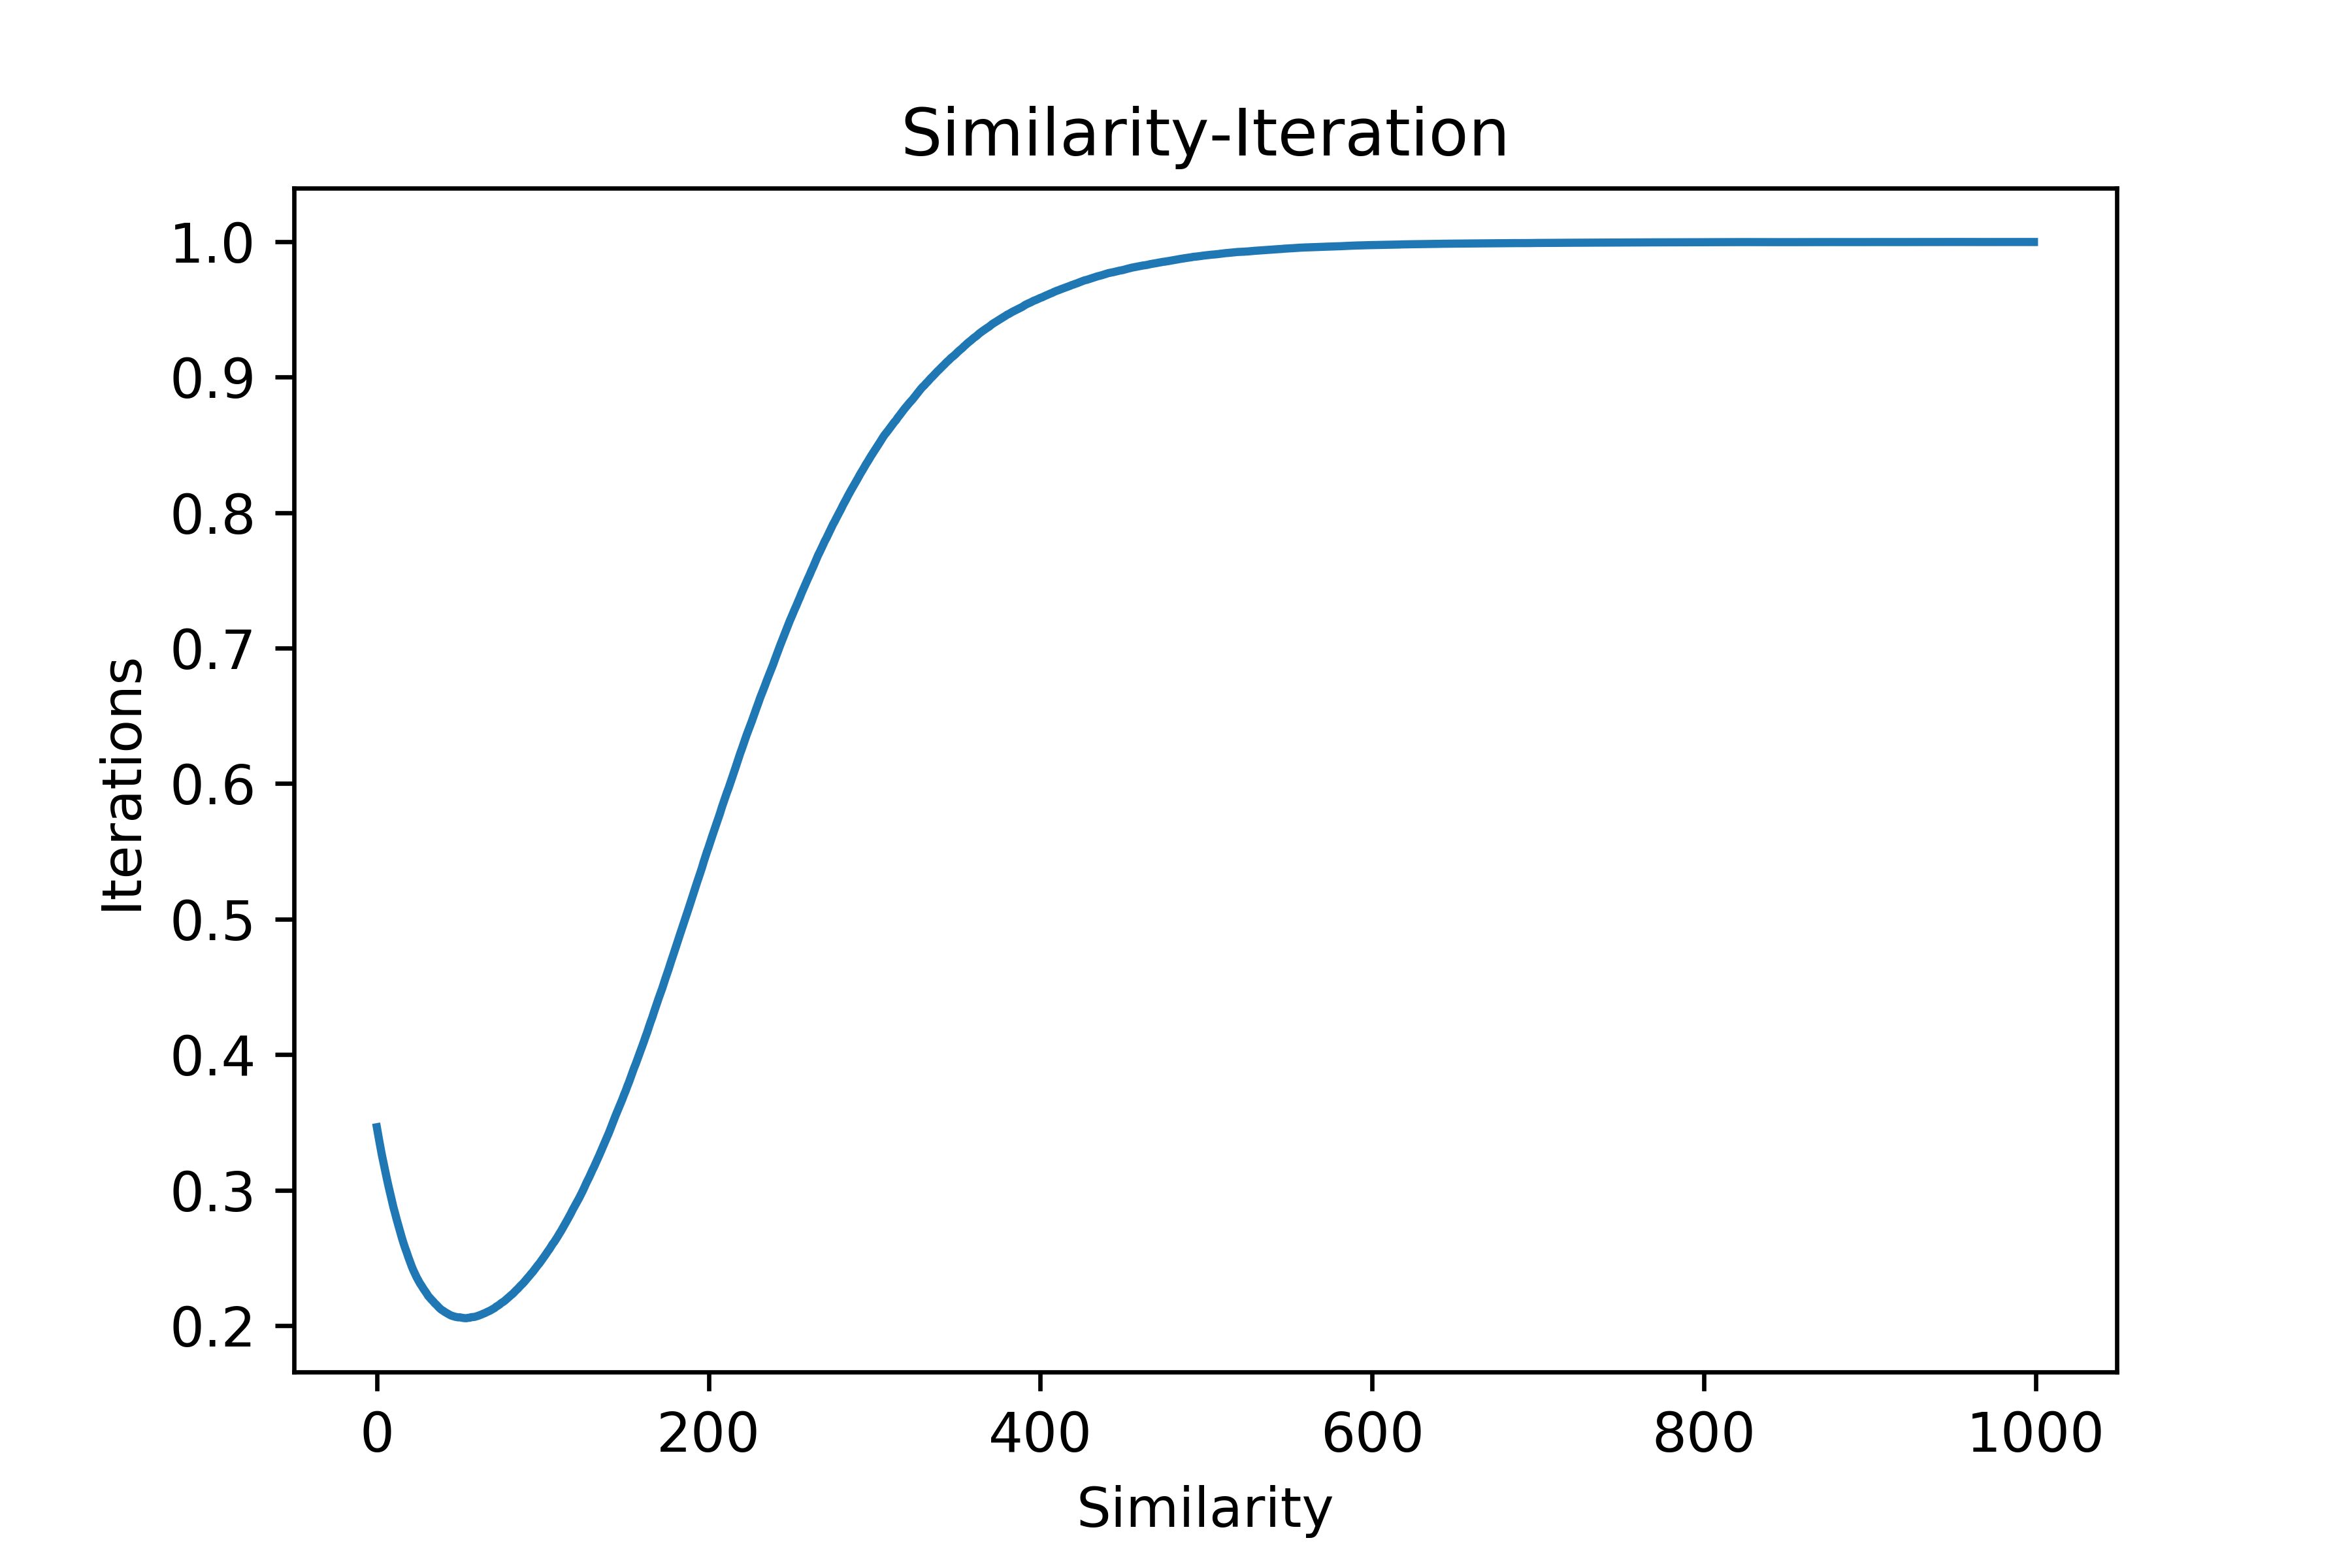
\includegraphics[width=0.9\textwidth]{Sim50_4_1000_1500_e3}
    	\caption{Similarity}\label{Sim50_4_1000_1500_e3}
    \end{figure}
    %
    \begin{figure}[H]
    	\centering
    	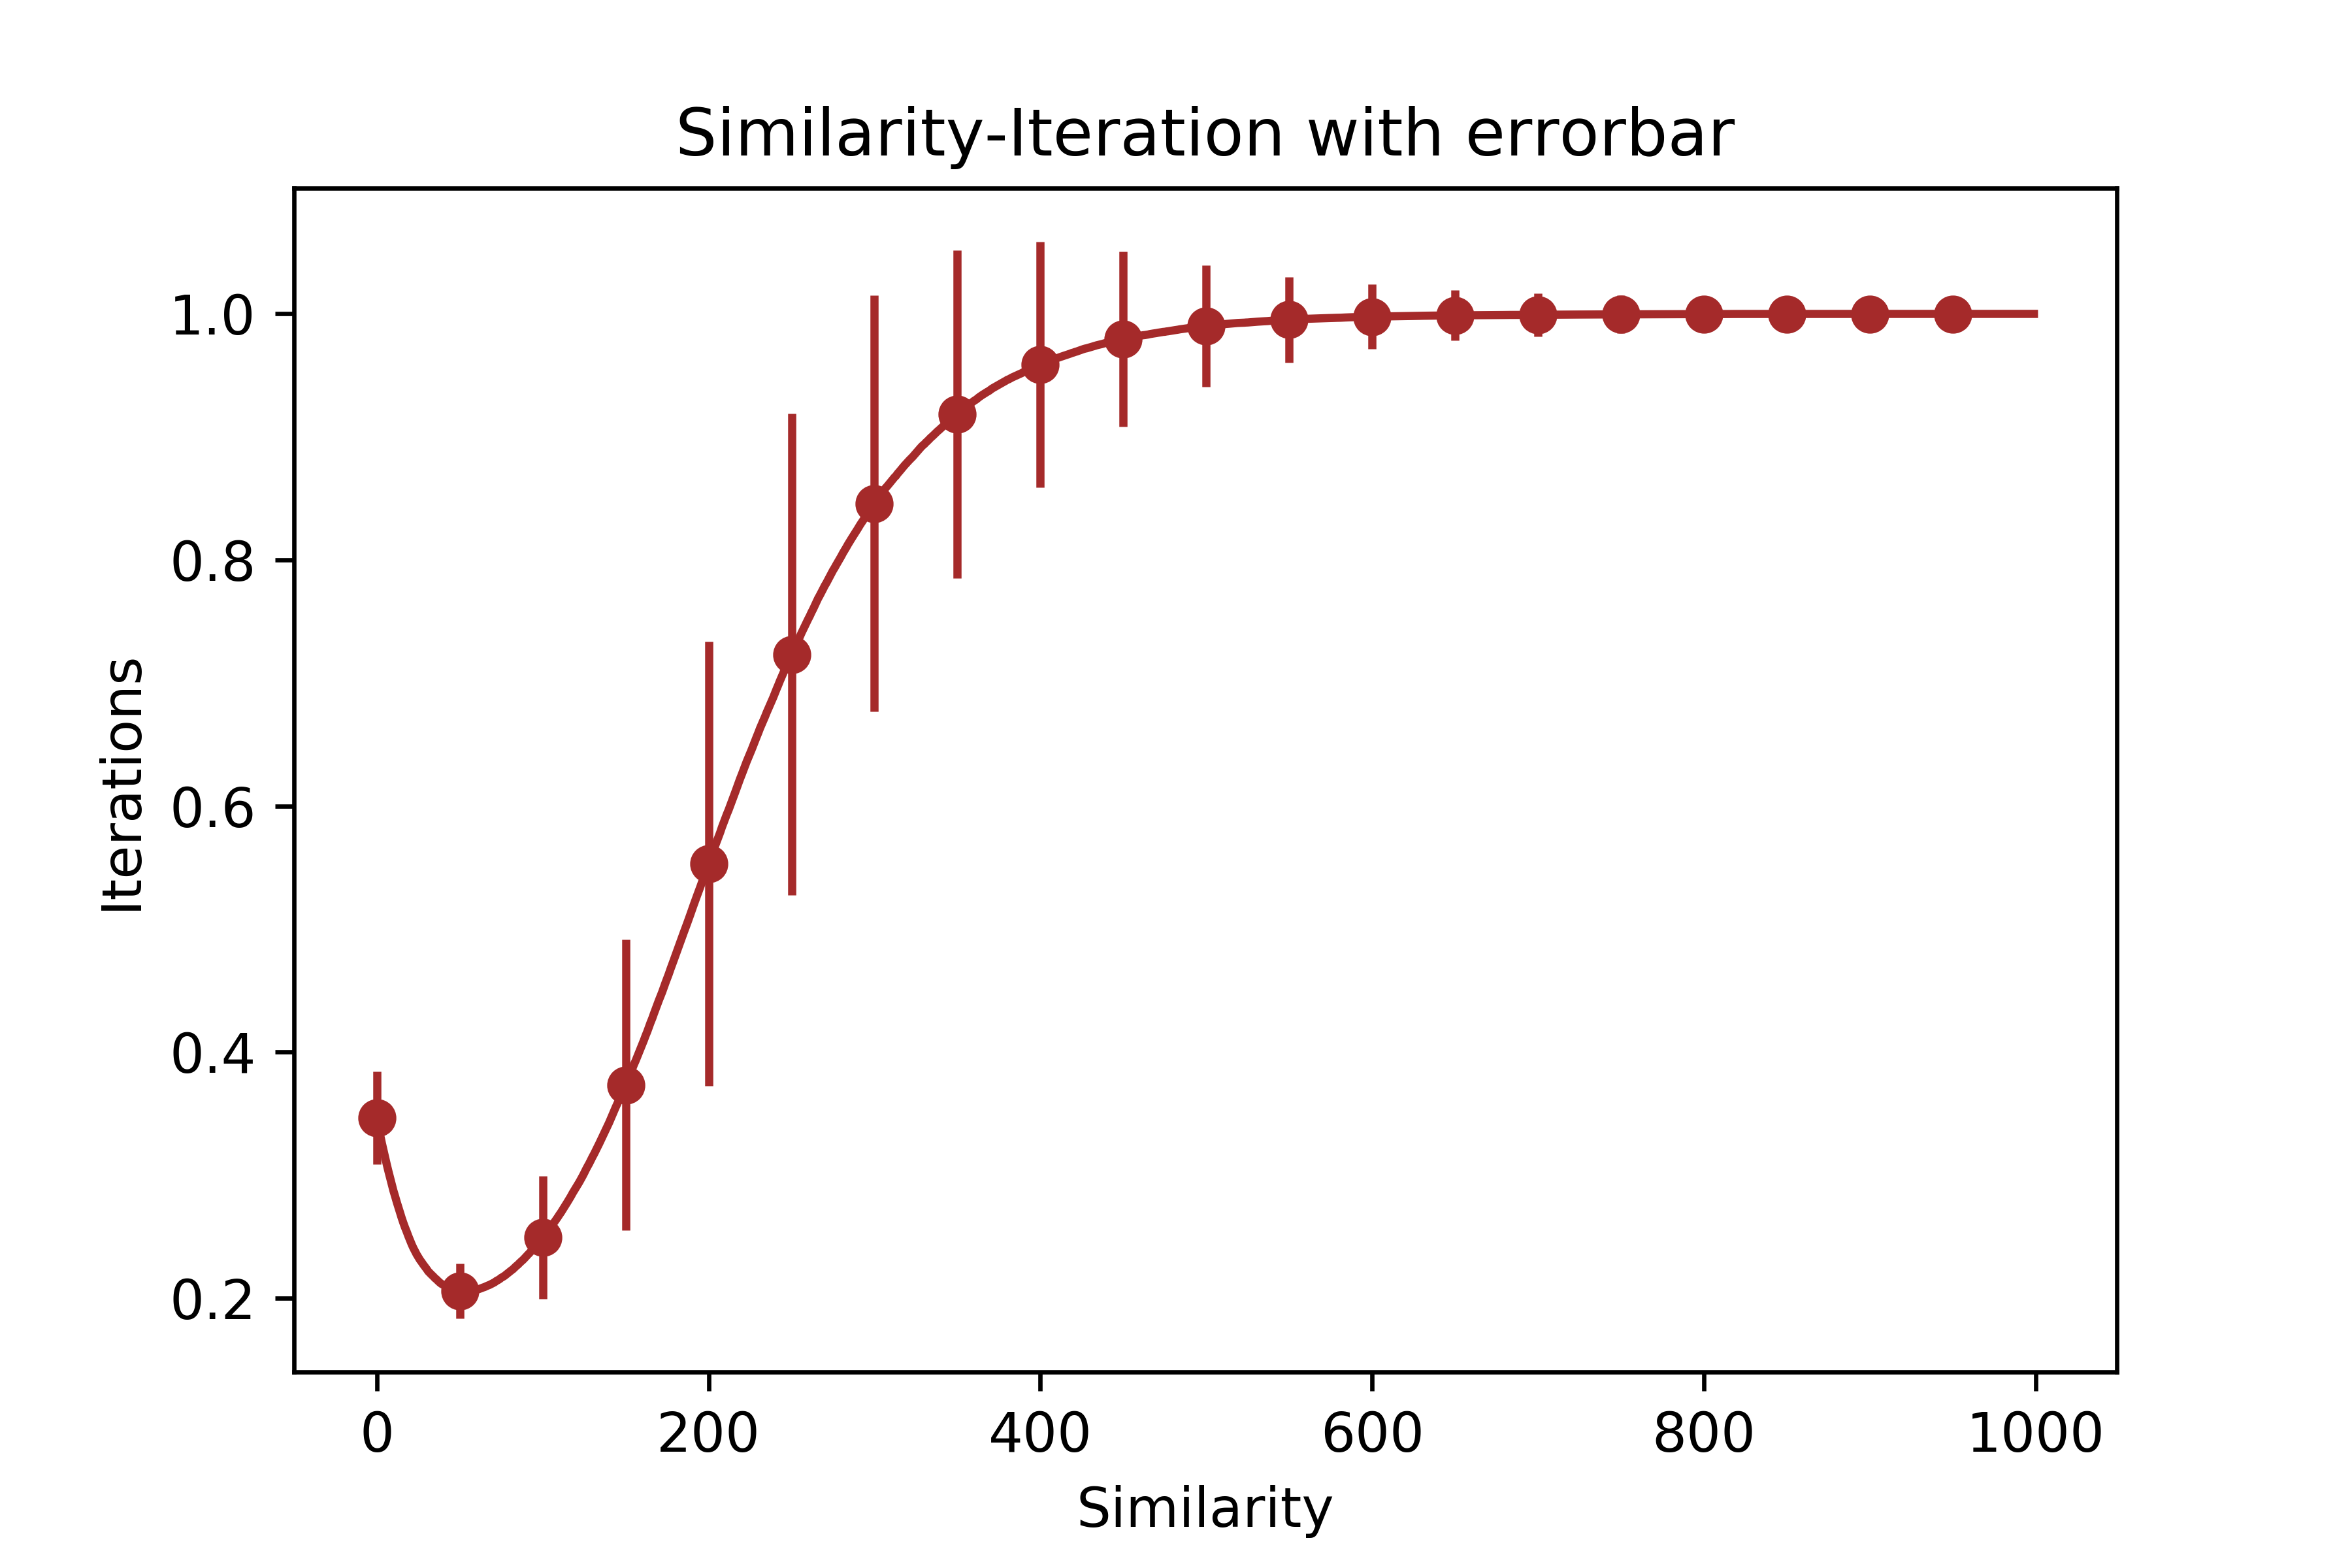
\includegraphics[width=0.9\textwidth]{SimErr50_4_1000_1500_e3}
    	\caption{Similarity with error bar}\label{SimErr50_4_1000_1500_e3}
    \end{figure}
    %
    \begin{figure}[H]
    	\centering
    	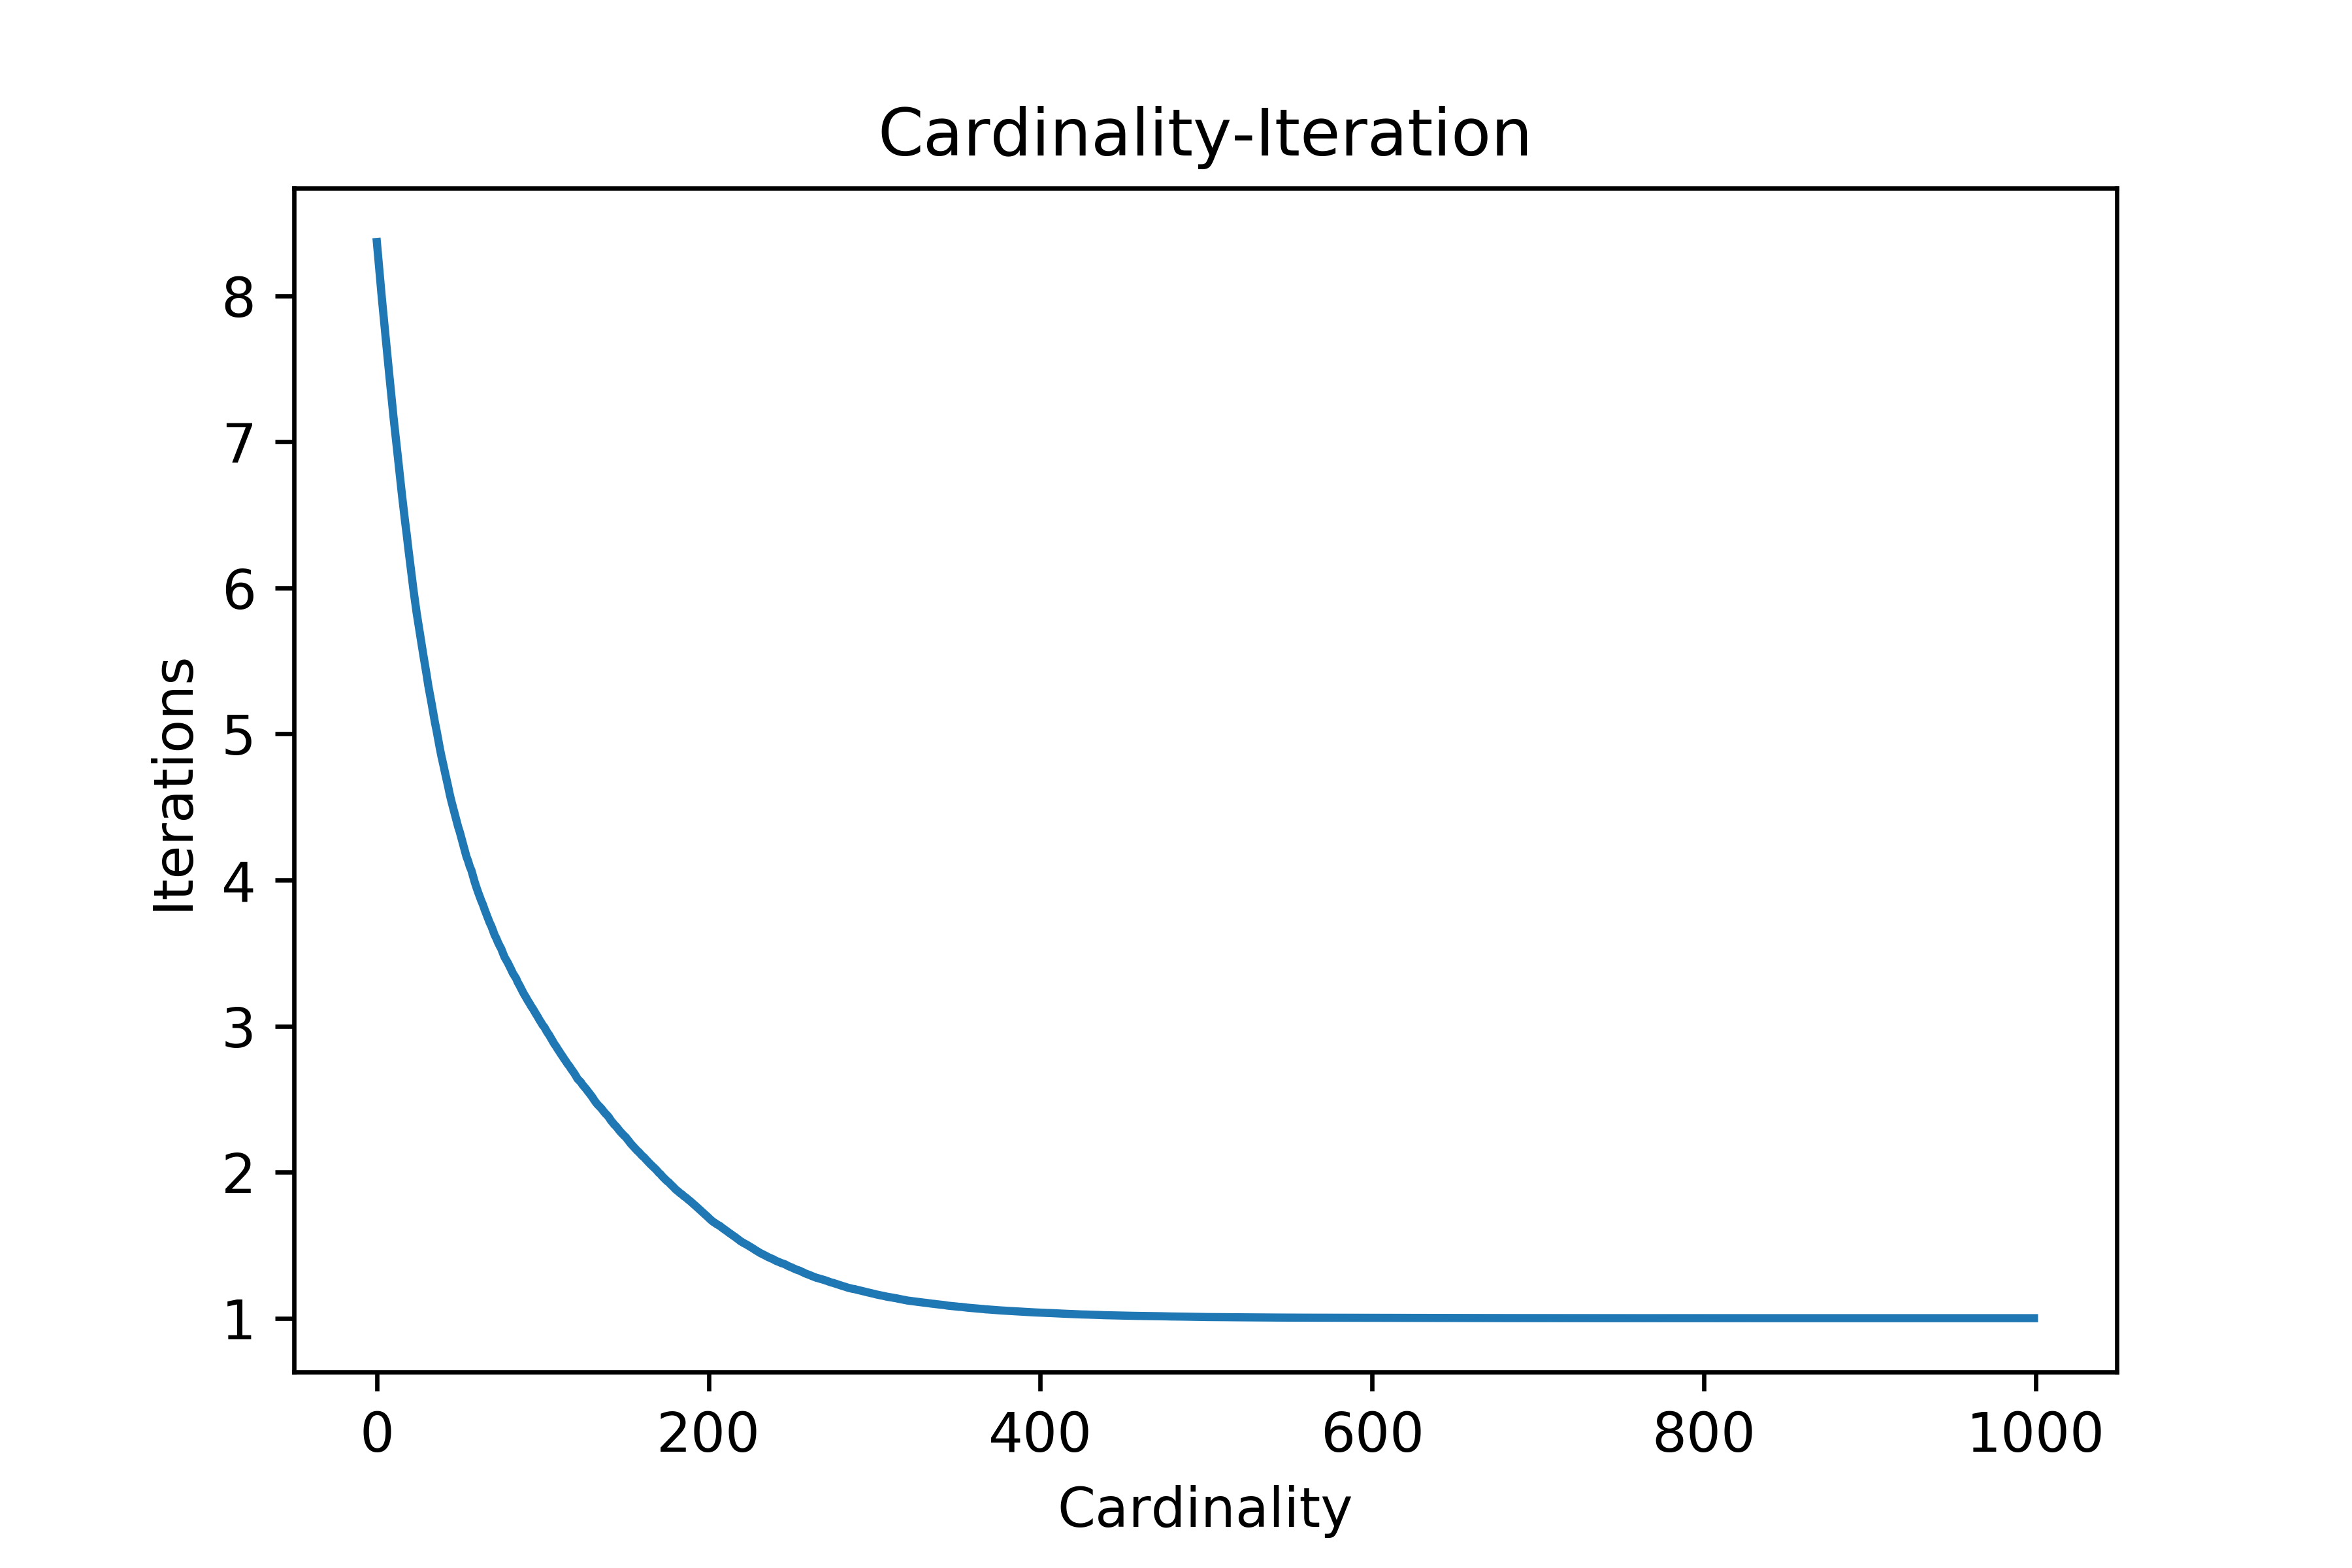
\includegraphics[width=0.9\textwidth]{Card50_4_1000_1500_e3}
    	\caption{Cardinality}\label{Card50_4_1000_1500_e3}
    \end{figure}
    %
    \begin{figure}[H]
    	\centering
    	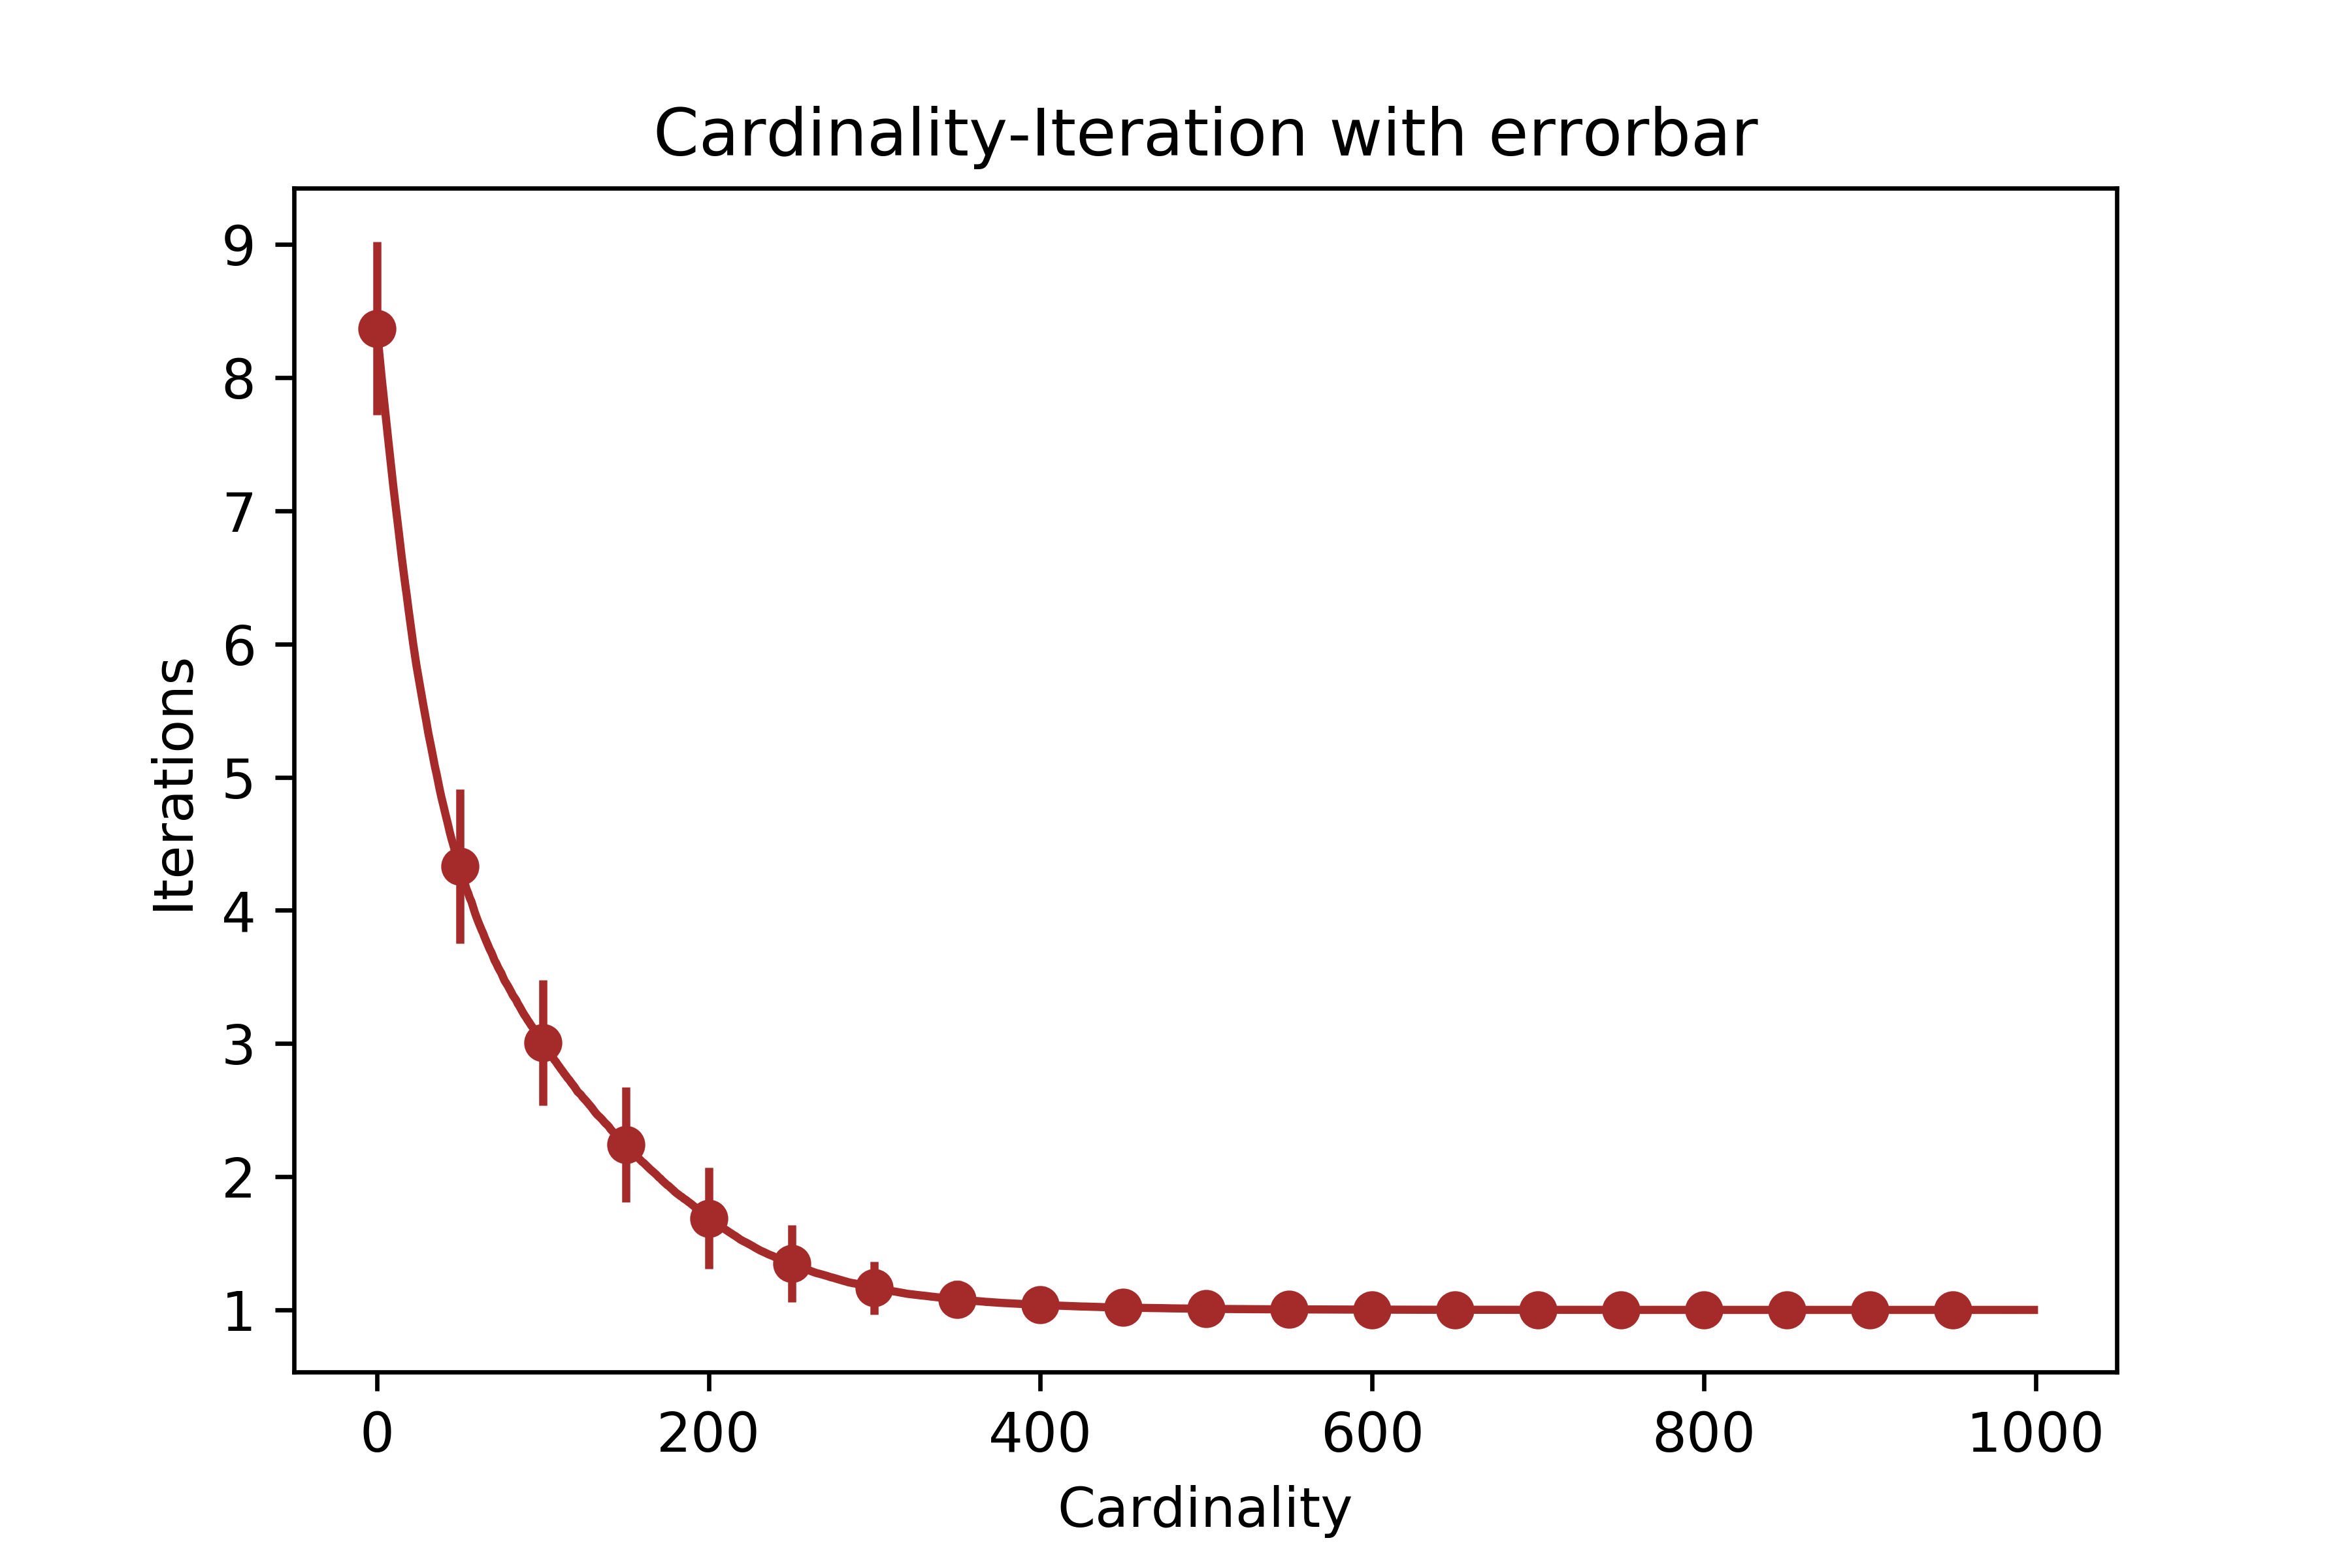
\includegraphics[width=0.9\textwidth]{CardErr50_4_1000_1500_e3}
    	\caption{Cardinality with error bar}\label{CardErr50_4_1000_1500_e3}
    \end{figure}
%%Section min Hamming Distance
	\section{Simulation Results with random initialise combine beliefs based on hamming distance(min)}
	the title: number of agents\_propositions\_iteration\_Times run\_threshold(Hamming distance)
    \graphicspath{{figsHamm/}}
    \subsection{50\_4\_1000\_100\_0.5}
    Time used: 84.14613086056161${s}$
       \begin{figure}[H]
    	\centering
    	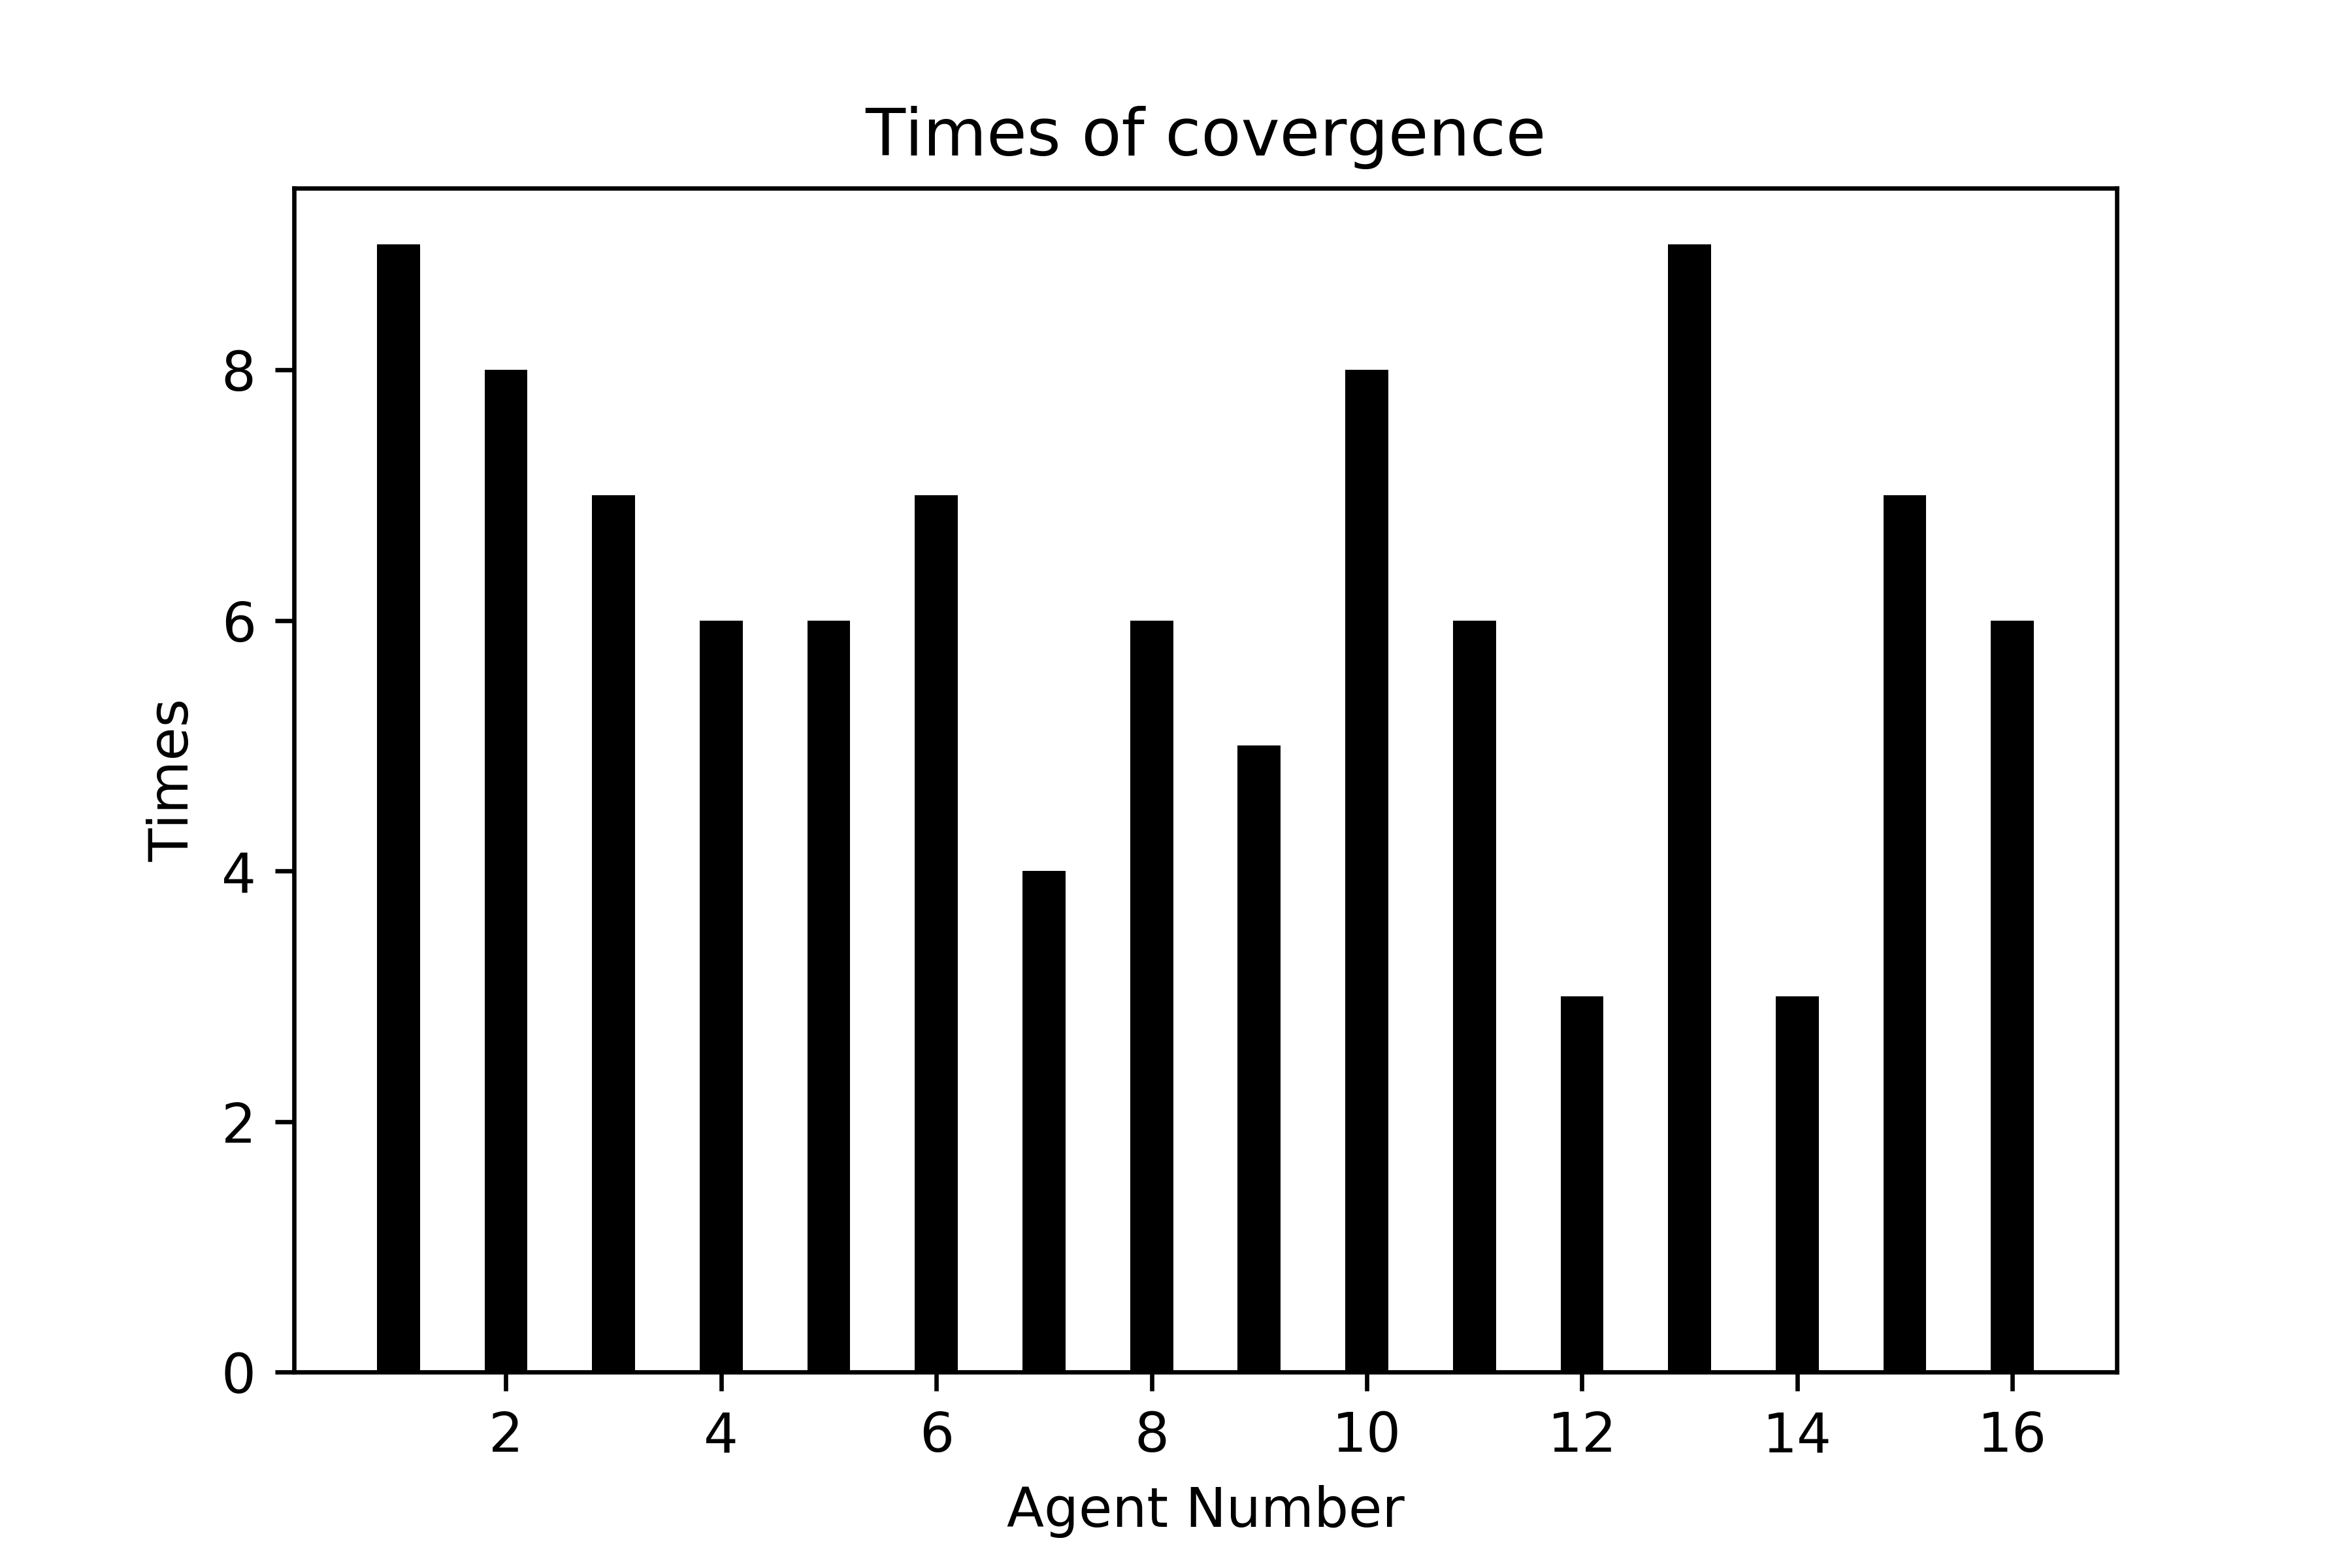
\includegraphics[width=0.9\textwidth]{agt50_4_1000_100_e3}
    	\caption{Where the iterations converge}\label{agt50_4_1000_100_e3_h}
    \end{figure}
    %
    \begin{figure}[H]
    	\centering
    	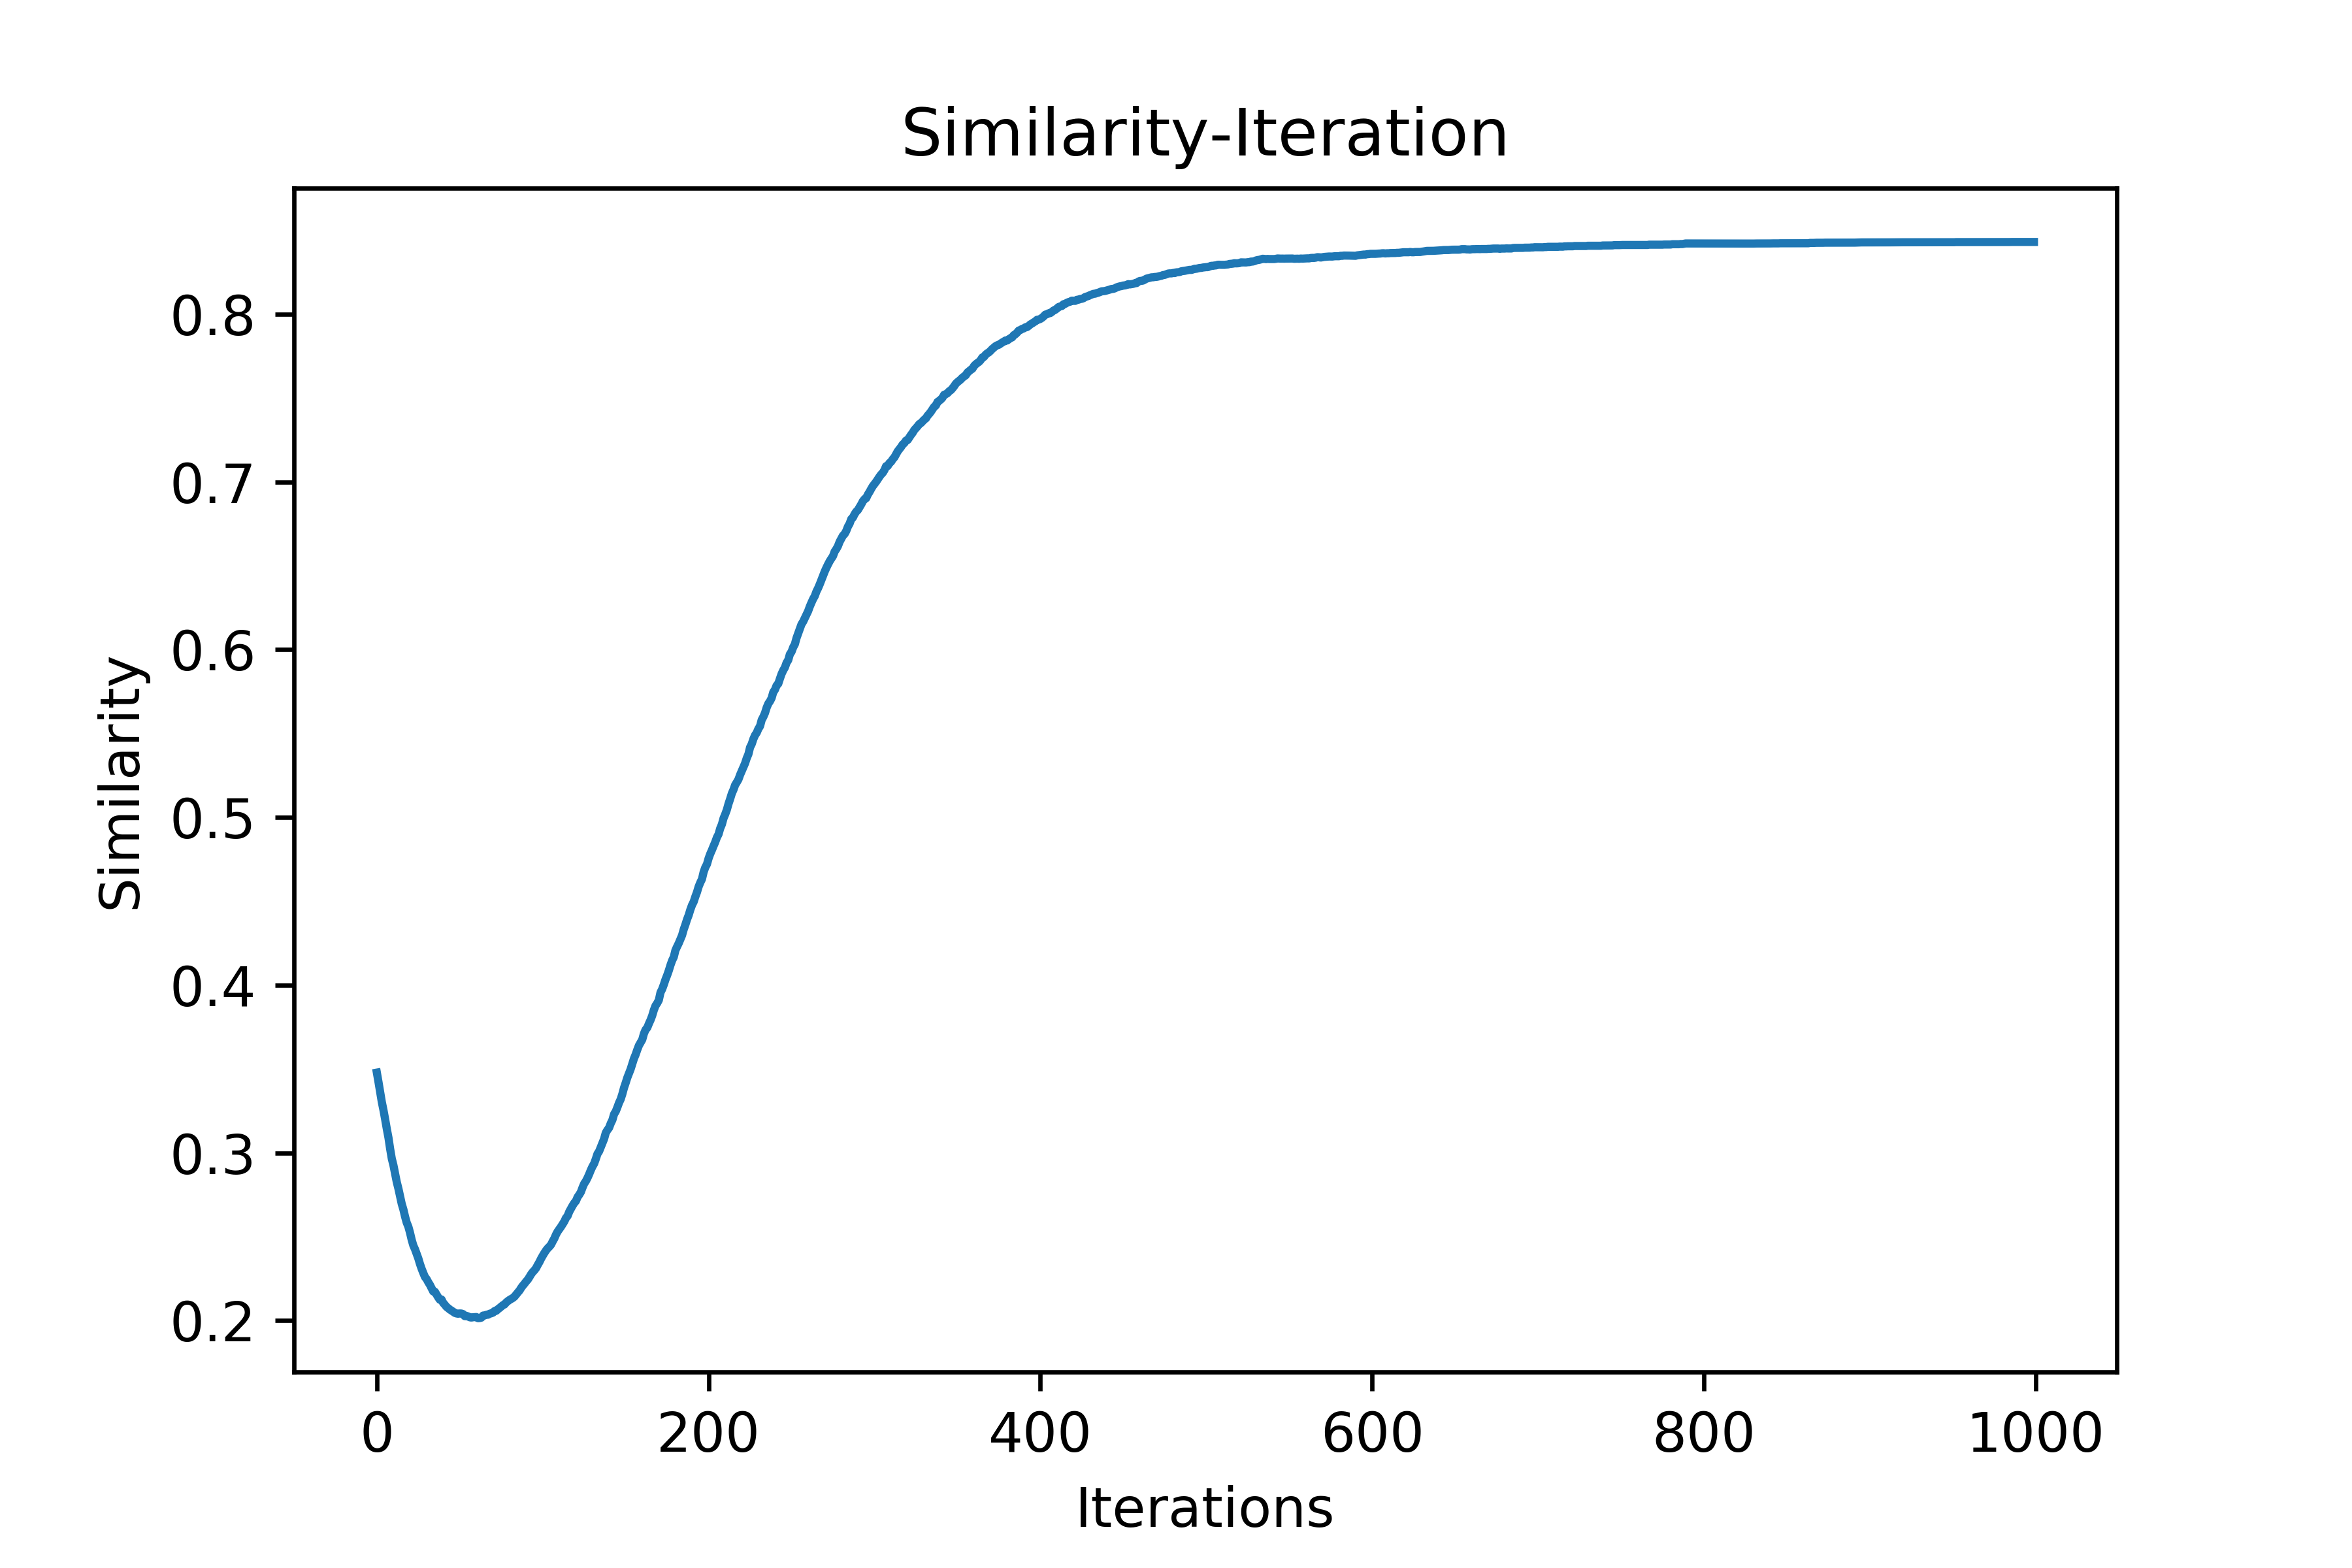
\includegraphics[width=0.9\textwidth]{Sim50_4_1000_100_e3}
    	\caption{Similarity}\label{Sim50_4_1000_100_e3_h}
    \end{figure}
    %
    \begin{figure}[H]
    	\centering
    	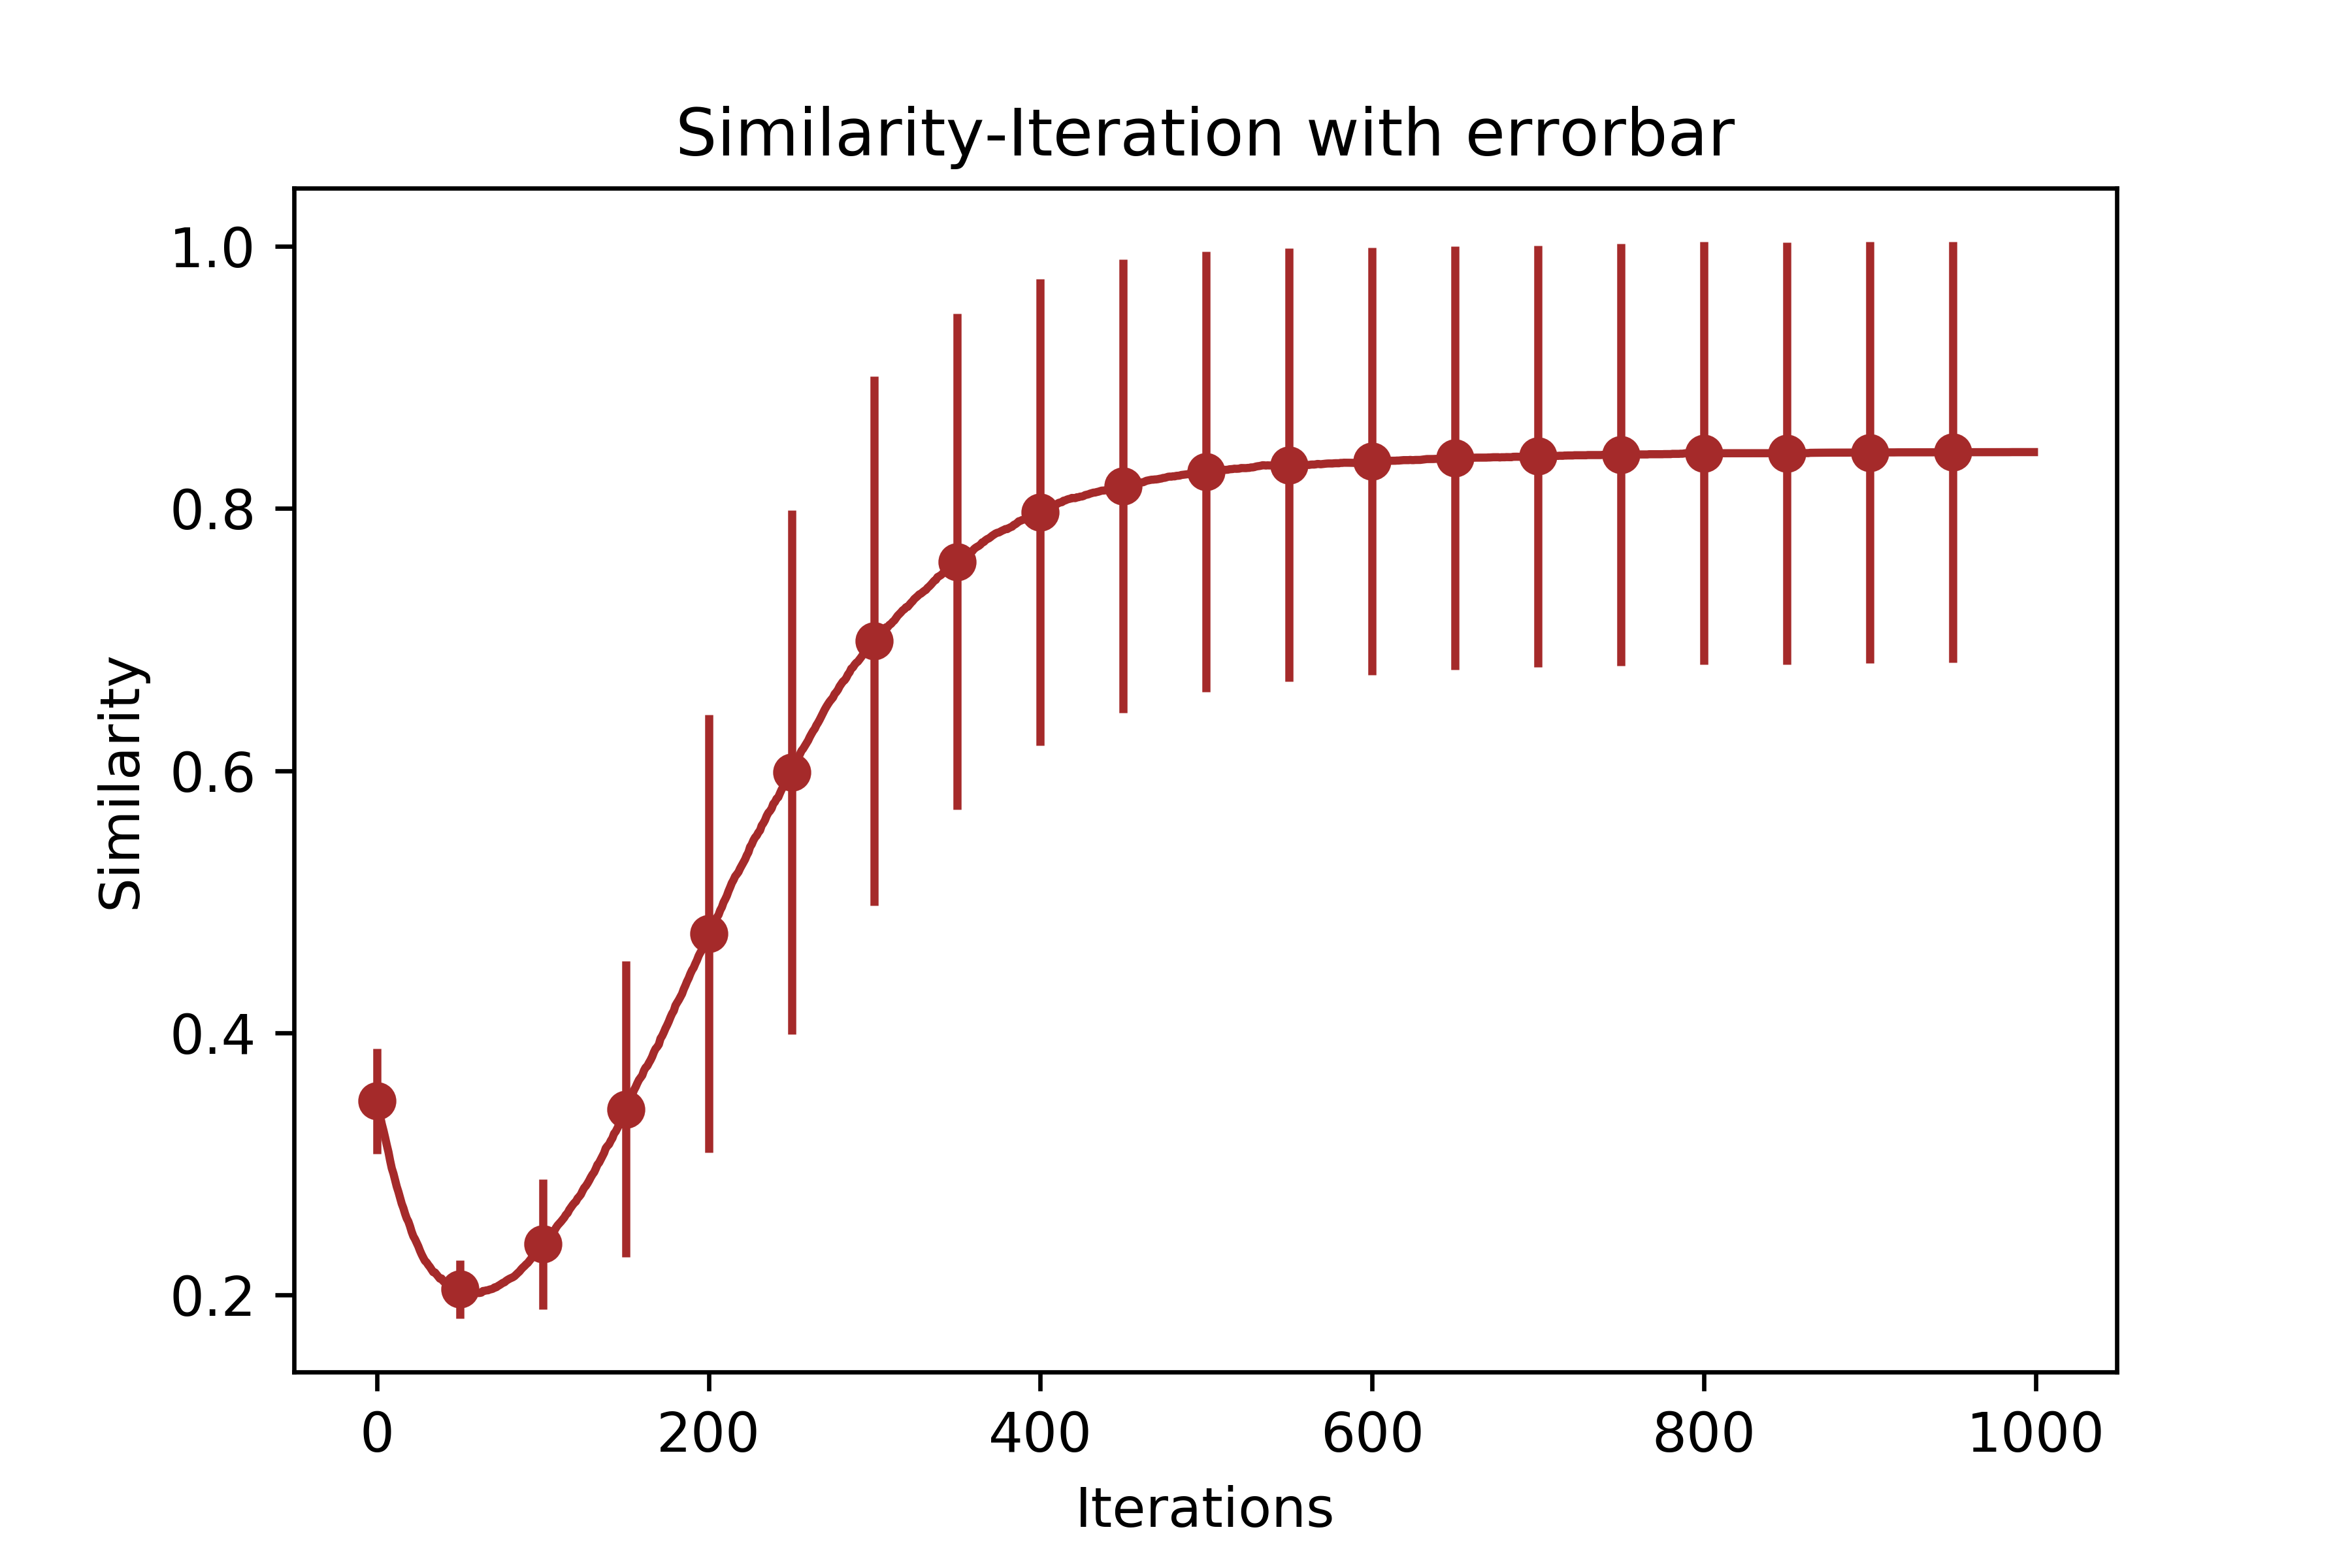
\includegraphics[width=0.9\textwidth]{SimErr50_4_1000_100_e3}
    	\caption{Similarity with error bar}\label{SimErr50_4_1000_100_e3_h}
    \end{figure}
    %
    \begin{figure}[H]
    	\centering
    	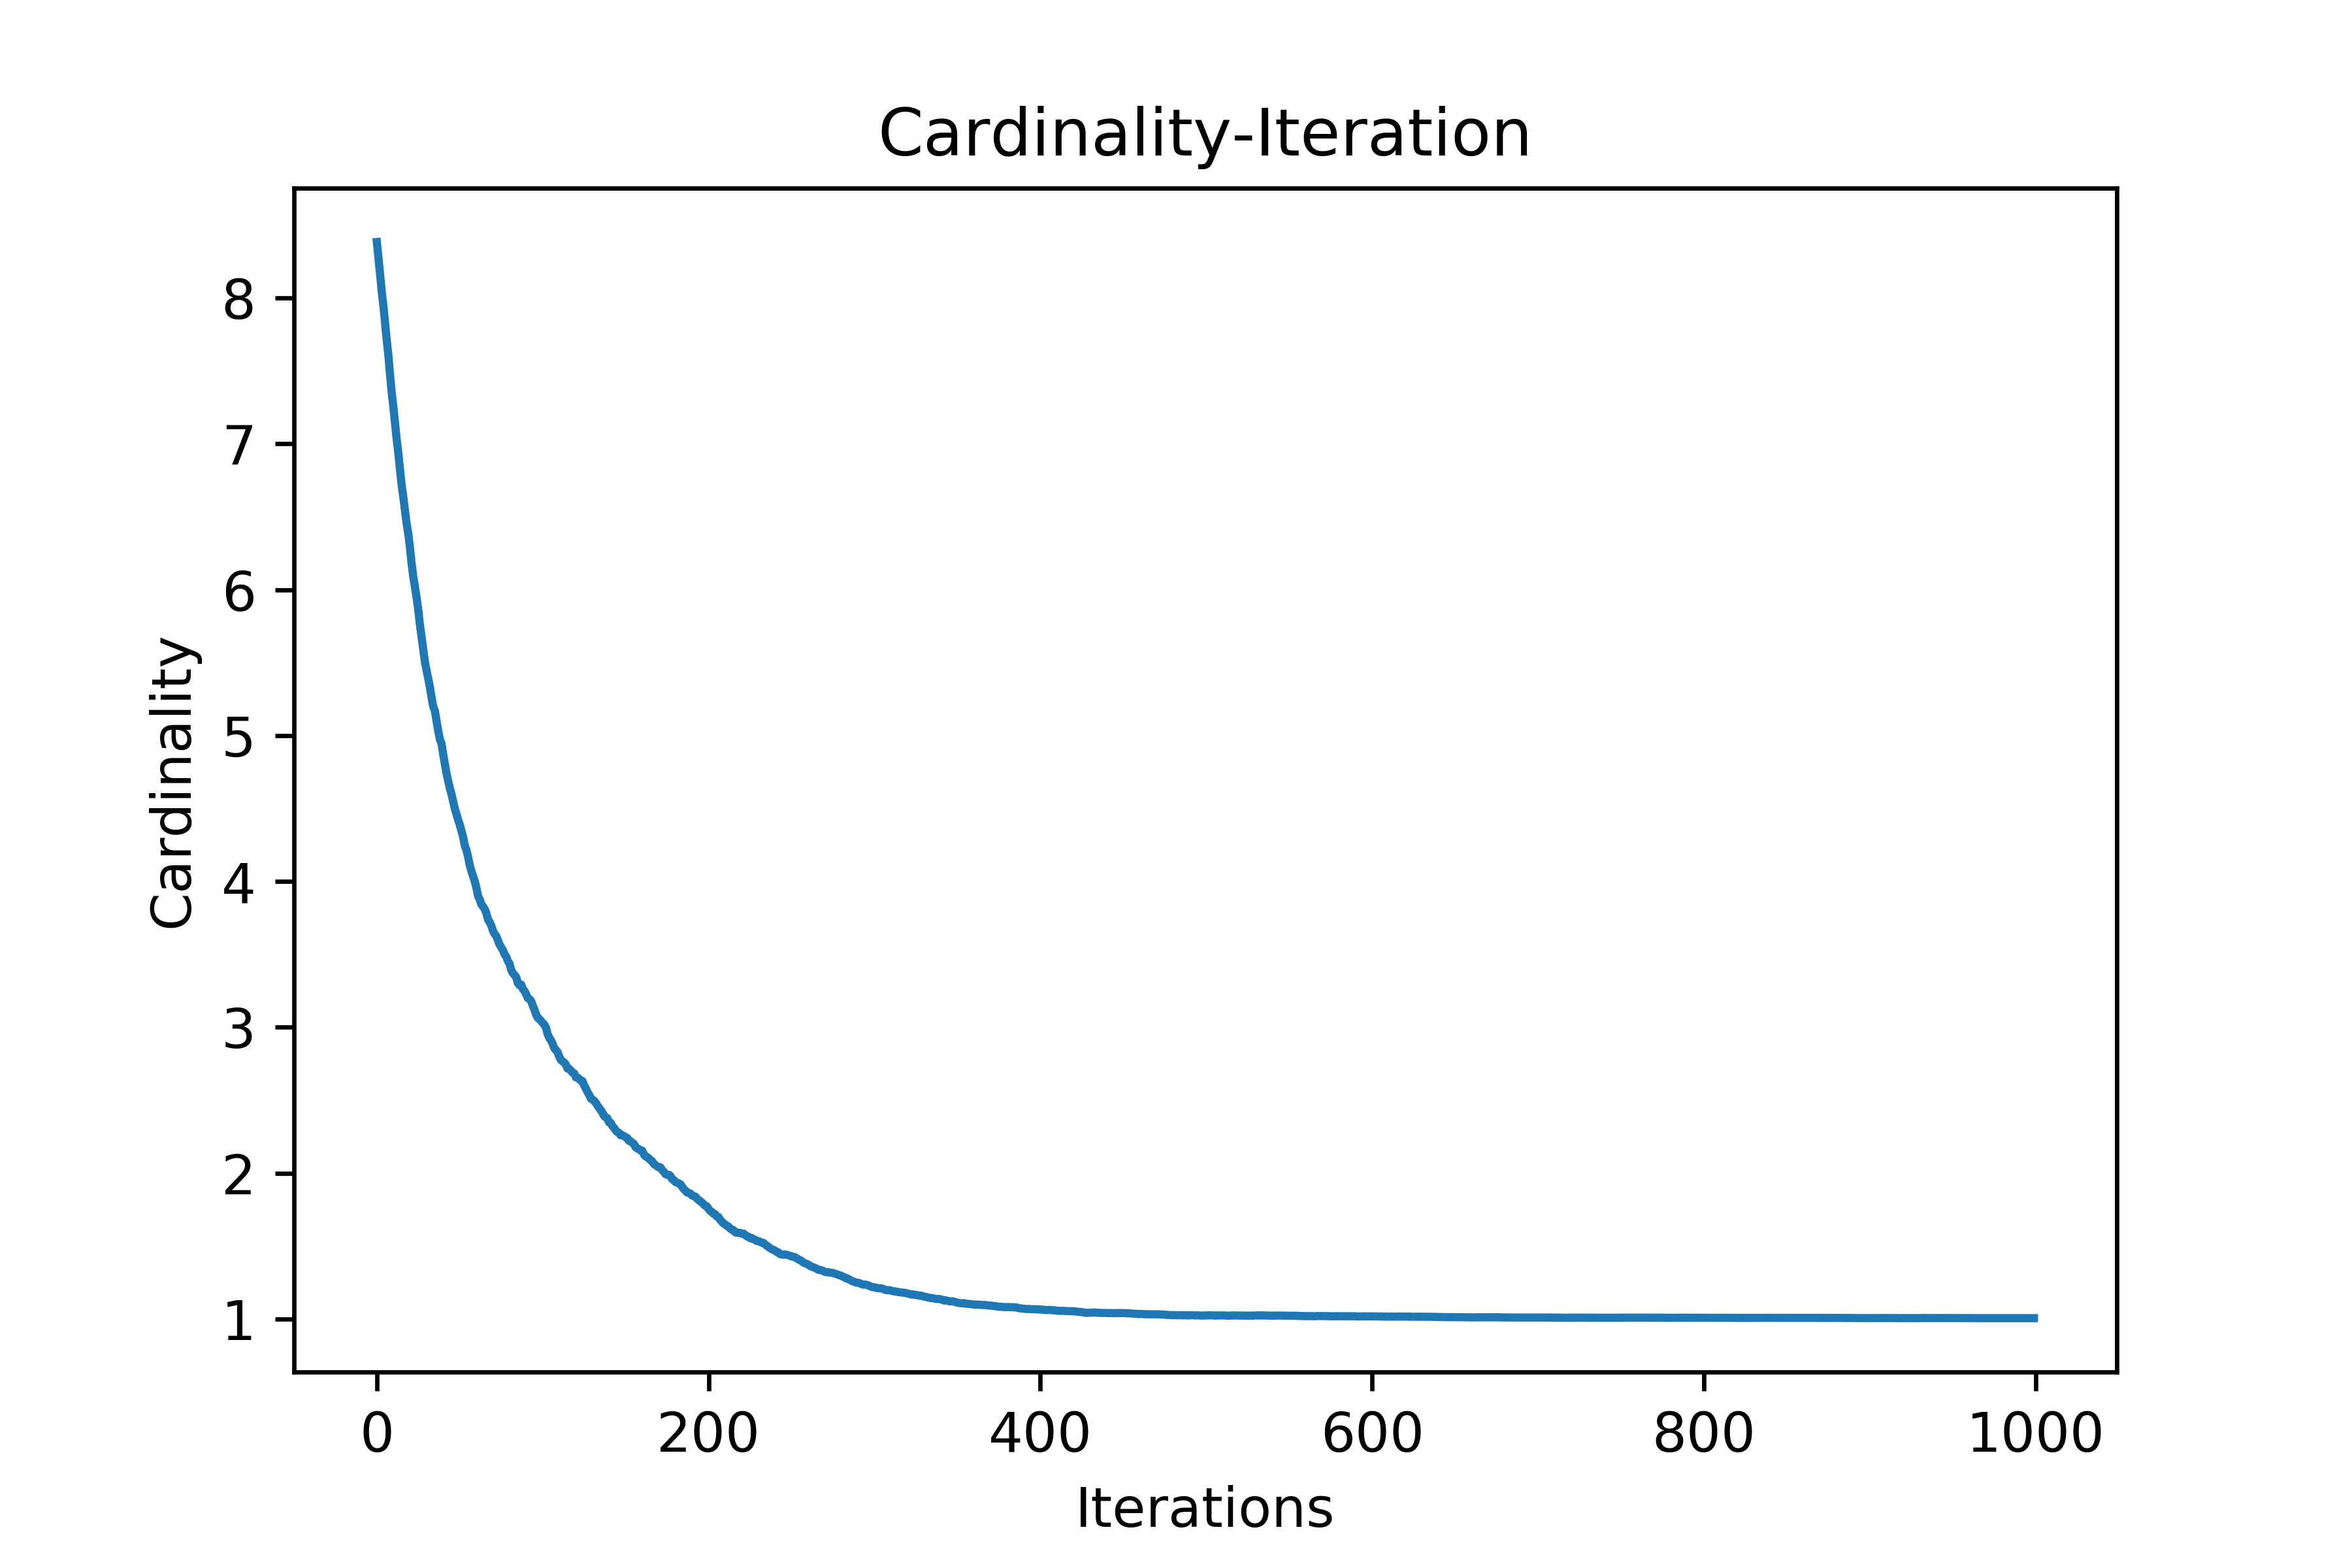
\includegraphics[width=0.9\textwidth]{Card50_4_1000_100_e3}
    	\caption{Cardinality}\label{Card50_4_1000_100_e3_h}
    \end{figure}
    %
    \begin{figure}[H]
    	\centering
    	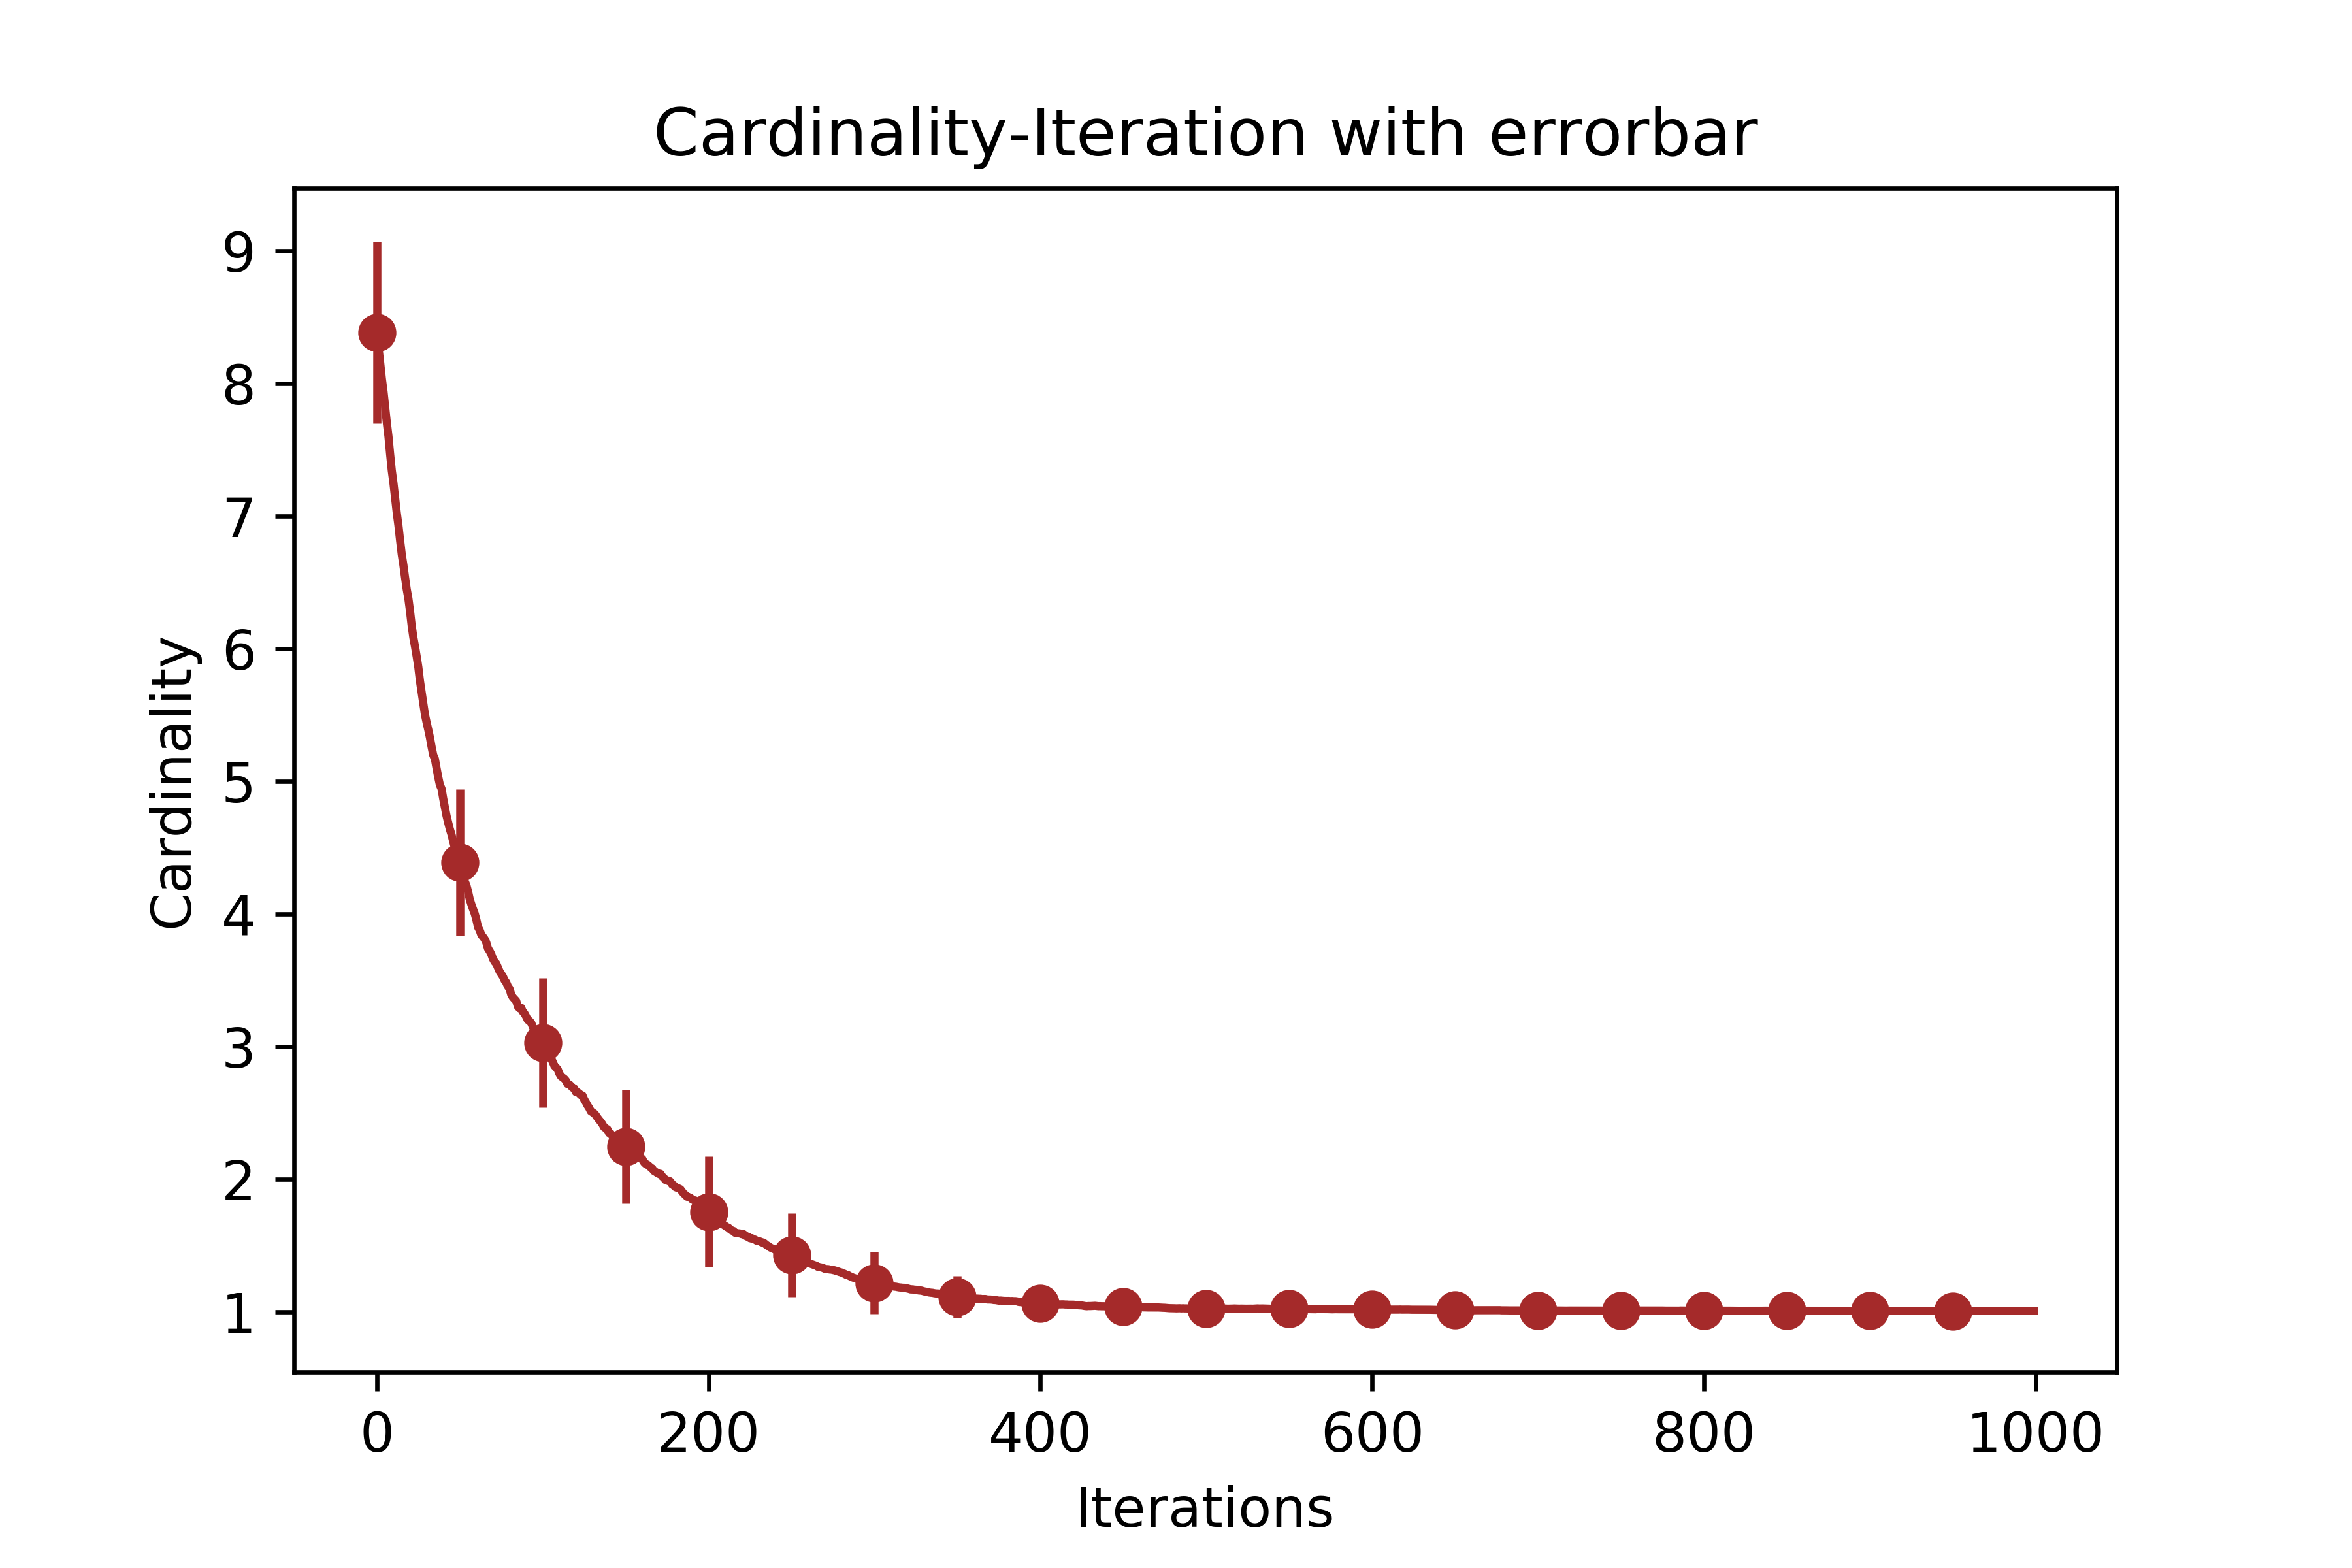
\includegraphics[width=0.9\textwidth]{CardErr50_4_1000_100_e3}
    	\caption{Cardinality with error bar}\label{CardErr50_4_1000_1500_e3_h}
    \end{figure}
        \begin{figure}[H]
    	\centering
    	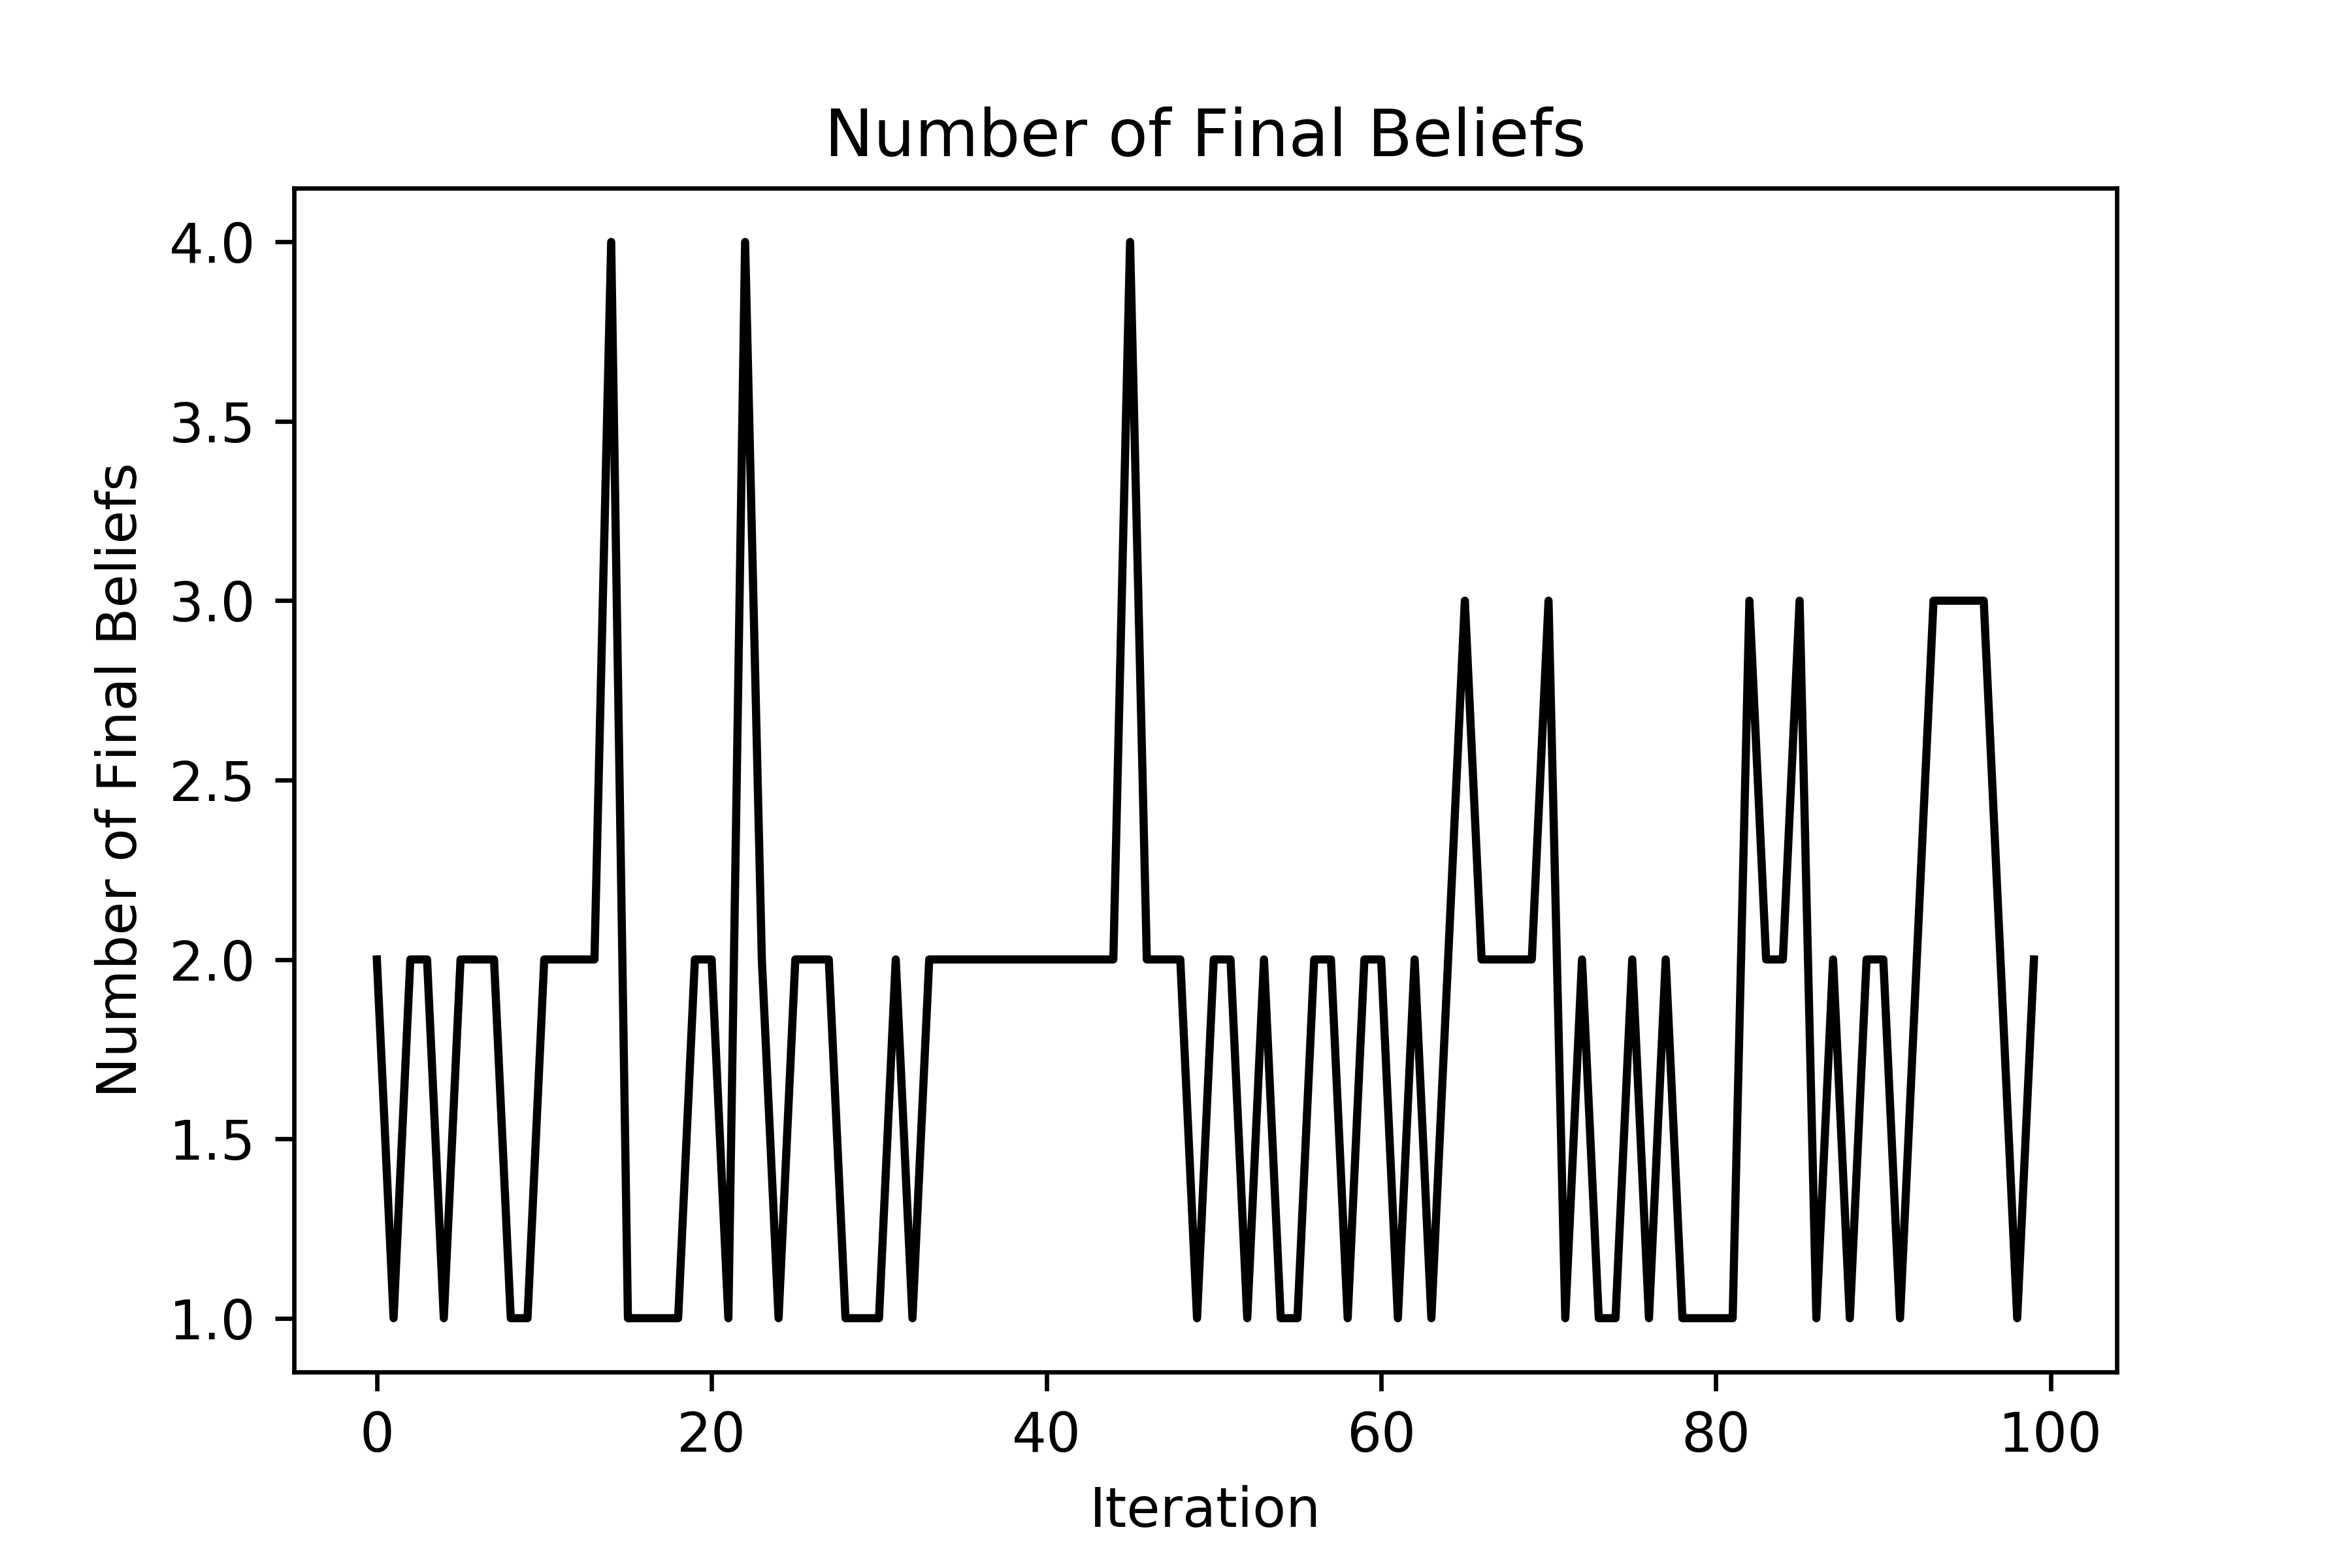
\includegraphics[width=0.9\textwidth]{numbef50_4_1000_100_e3}
    	\caption{Cardinality with error bar}\label{numbef50_4_1000_1500_e3_h}
    \end{figure}
        \subsection{50\_5\_1200\_100\_0.3}
    Time used: 107.05263902594515${s}$
    \begin{figure}[H]
    	\centering
    	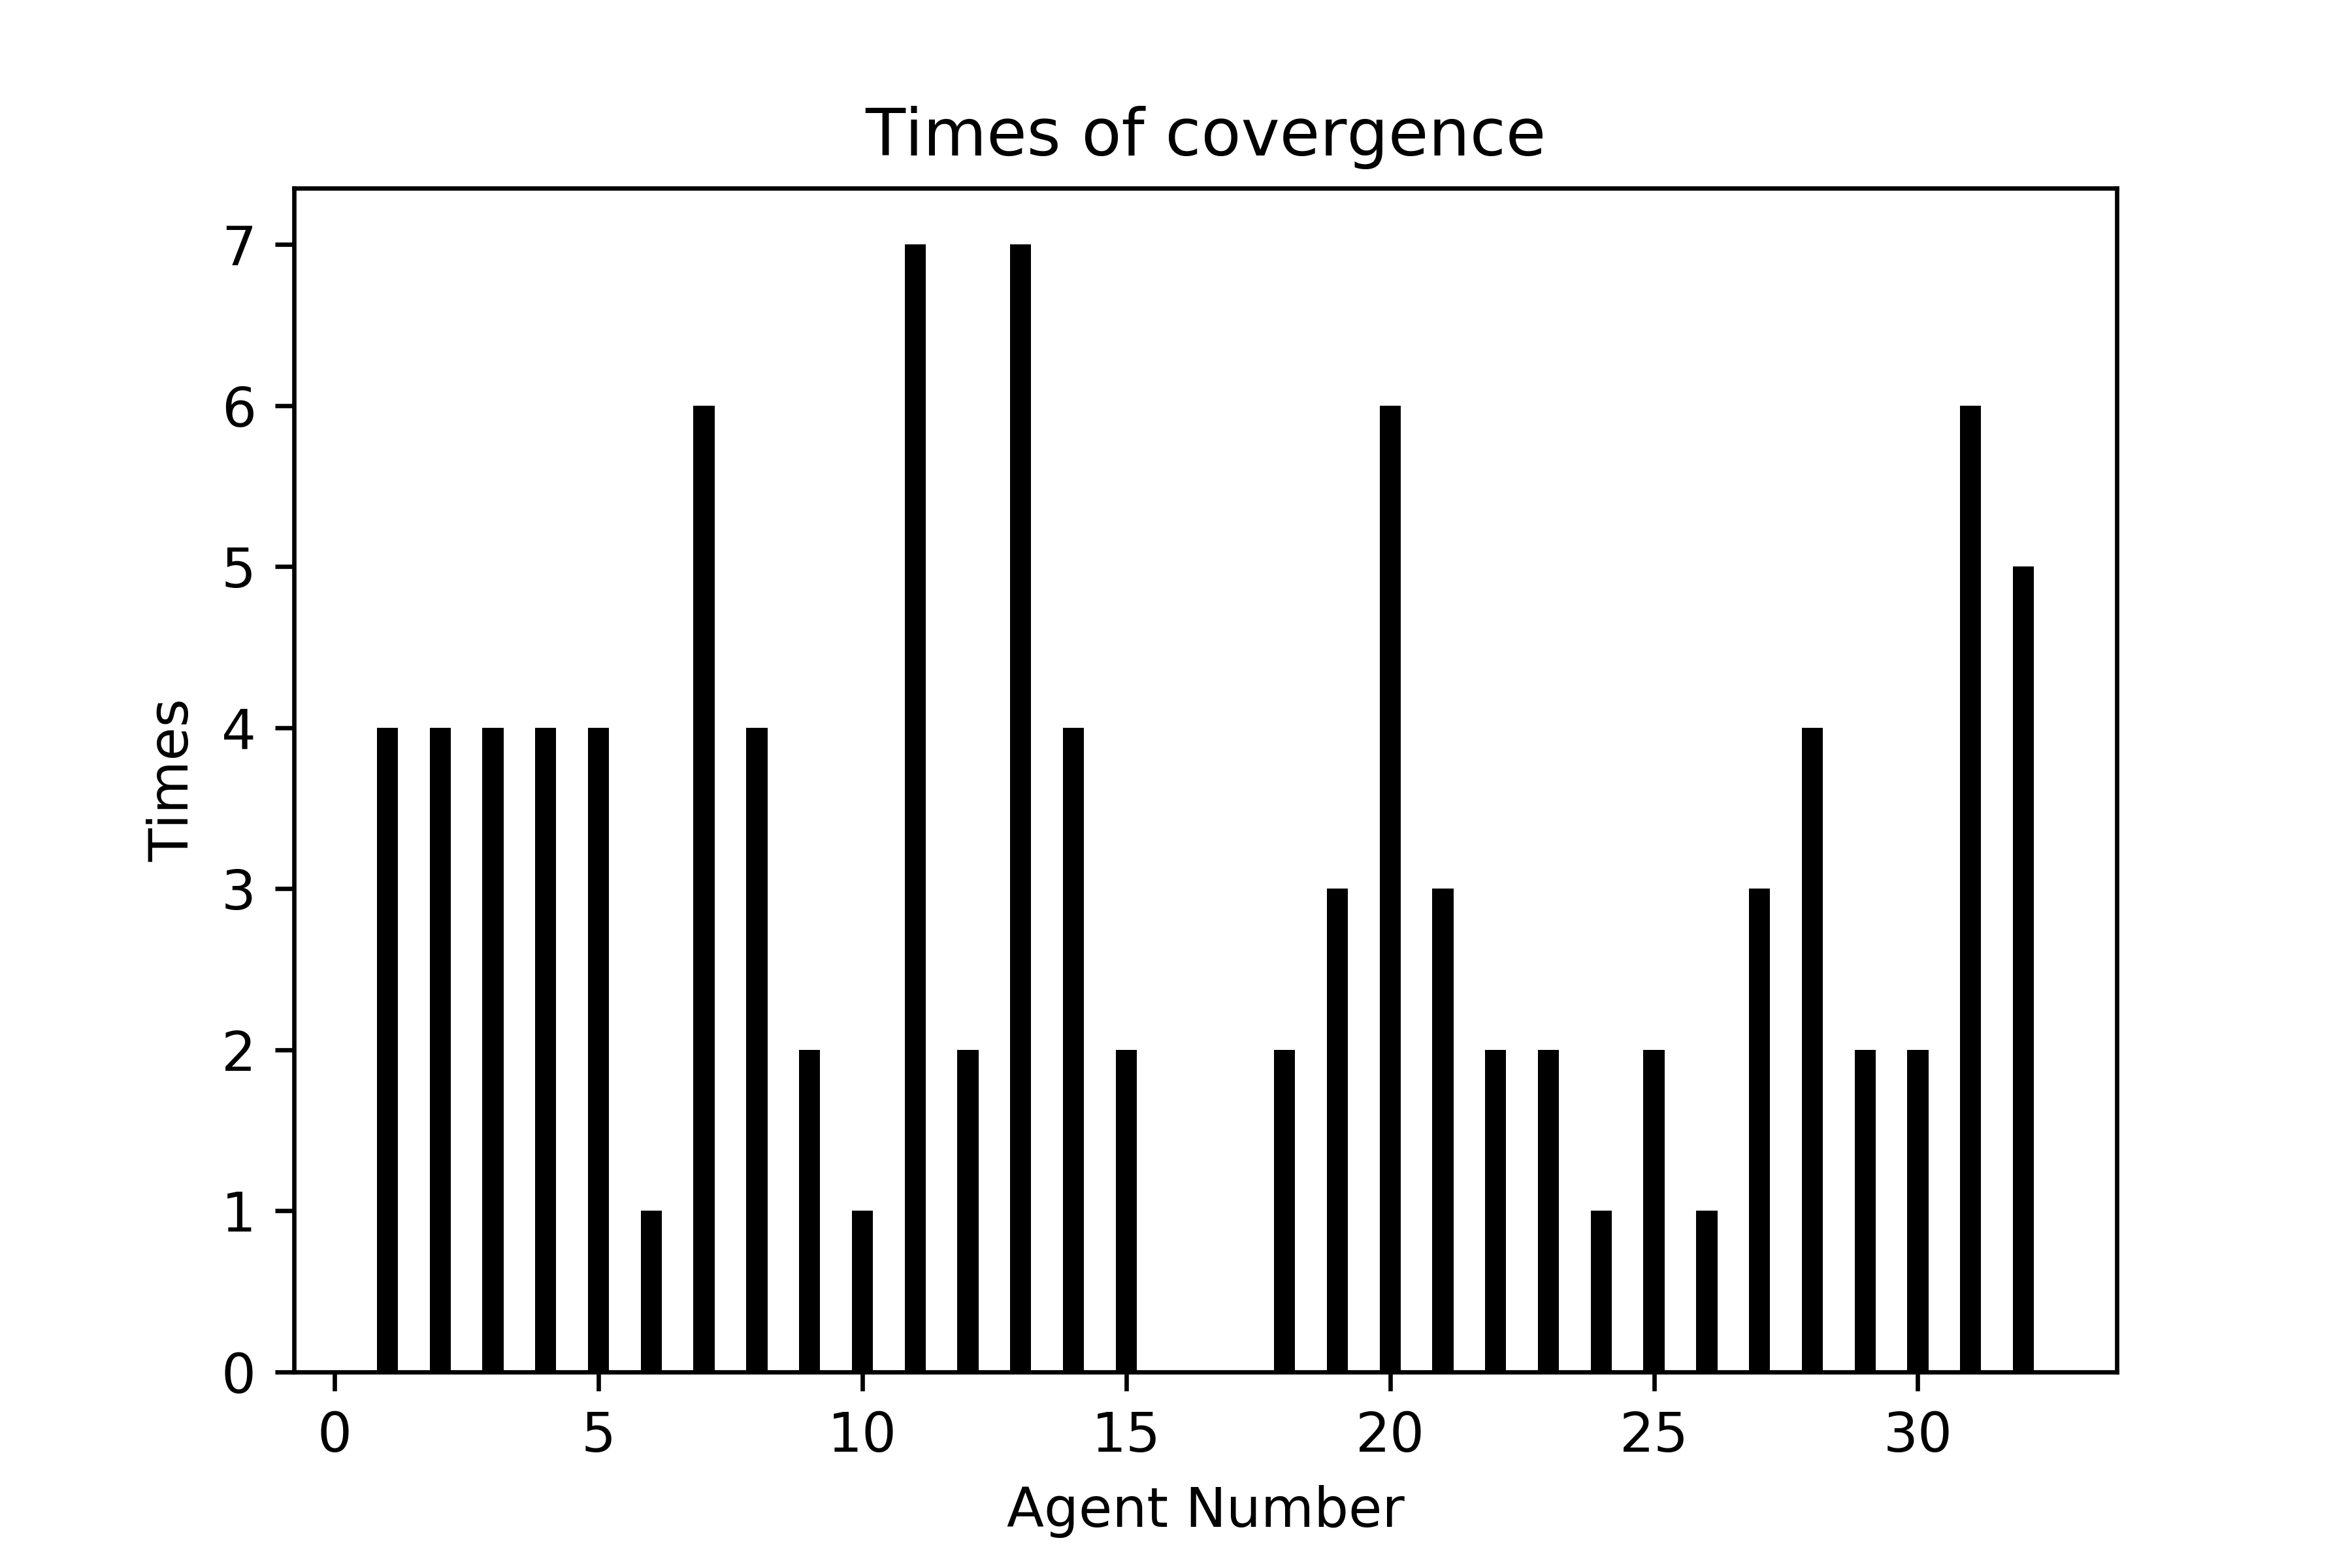
\includegraphics[width=0.9\textwidth]{agt50_5_1200_100_3.png}
    	\caption{Where the iterations converge}\label{agt50_5_1200_100_3_h}
    \end{figure}
    %
    \begin{figure}[H]
    	\centering
    	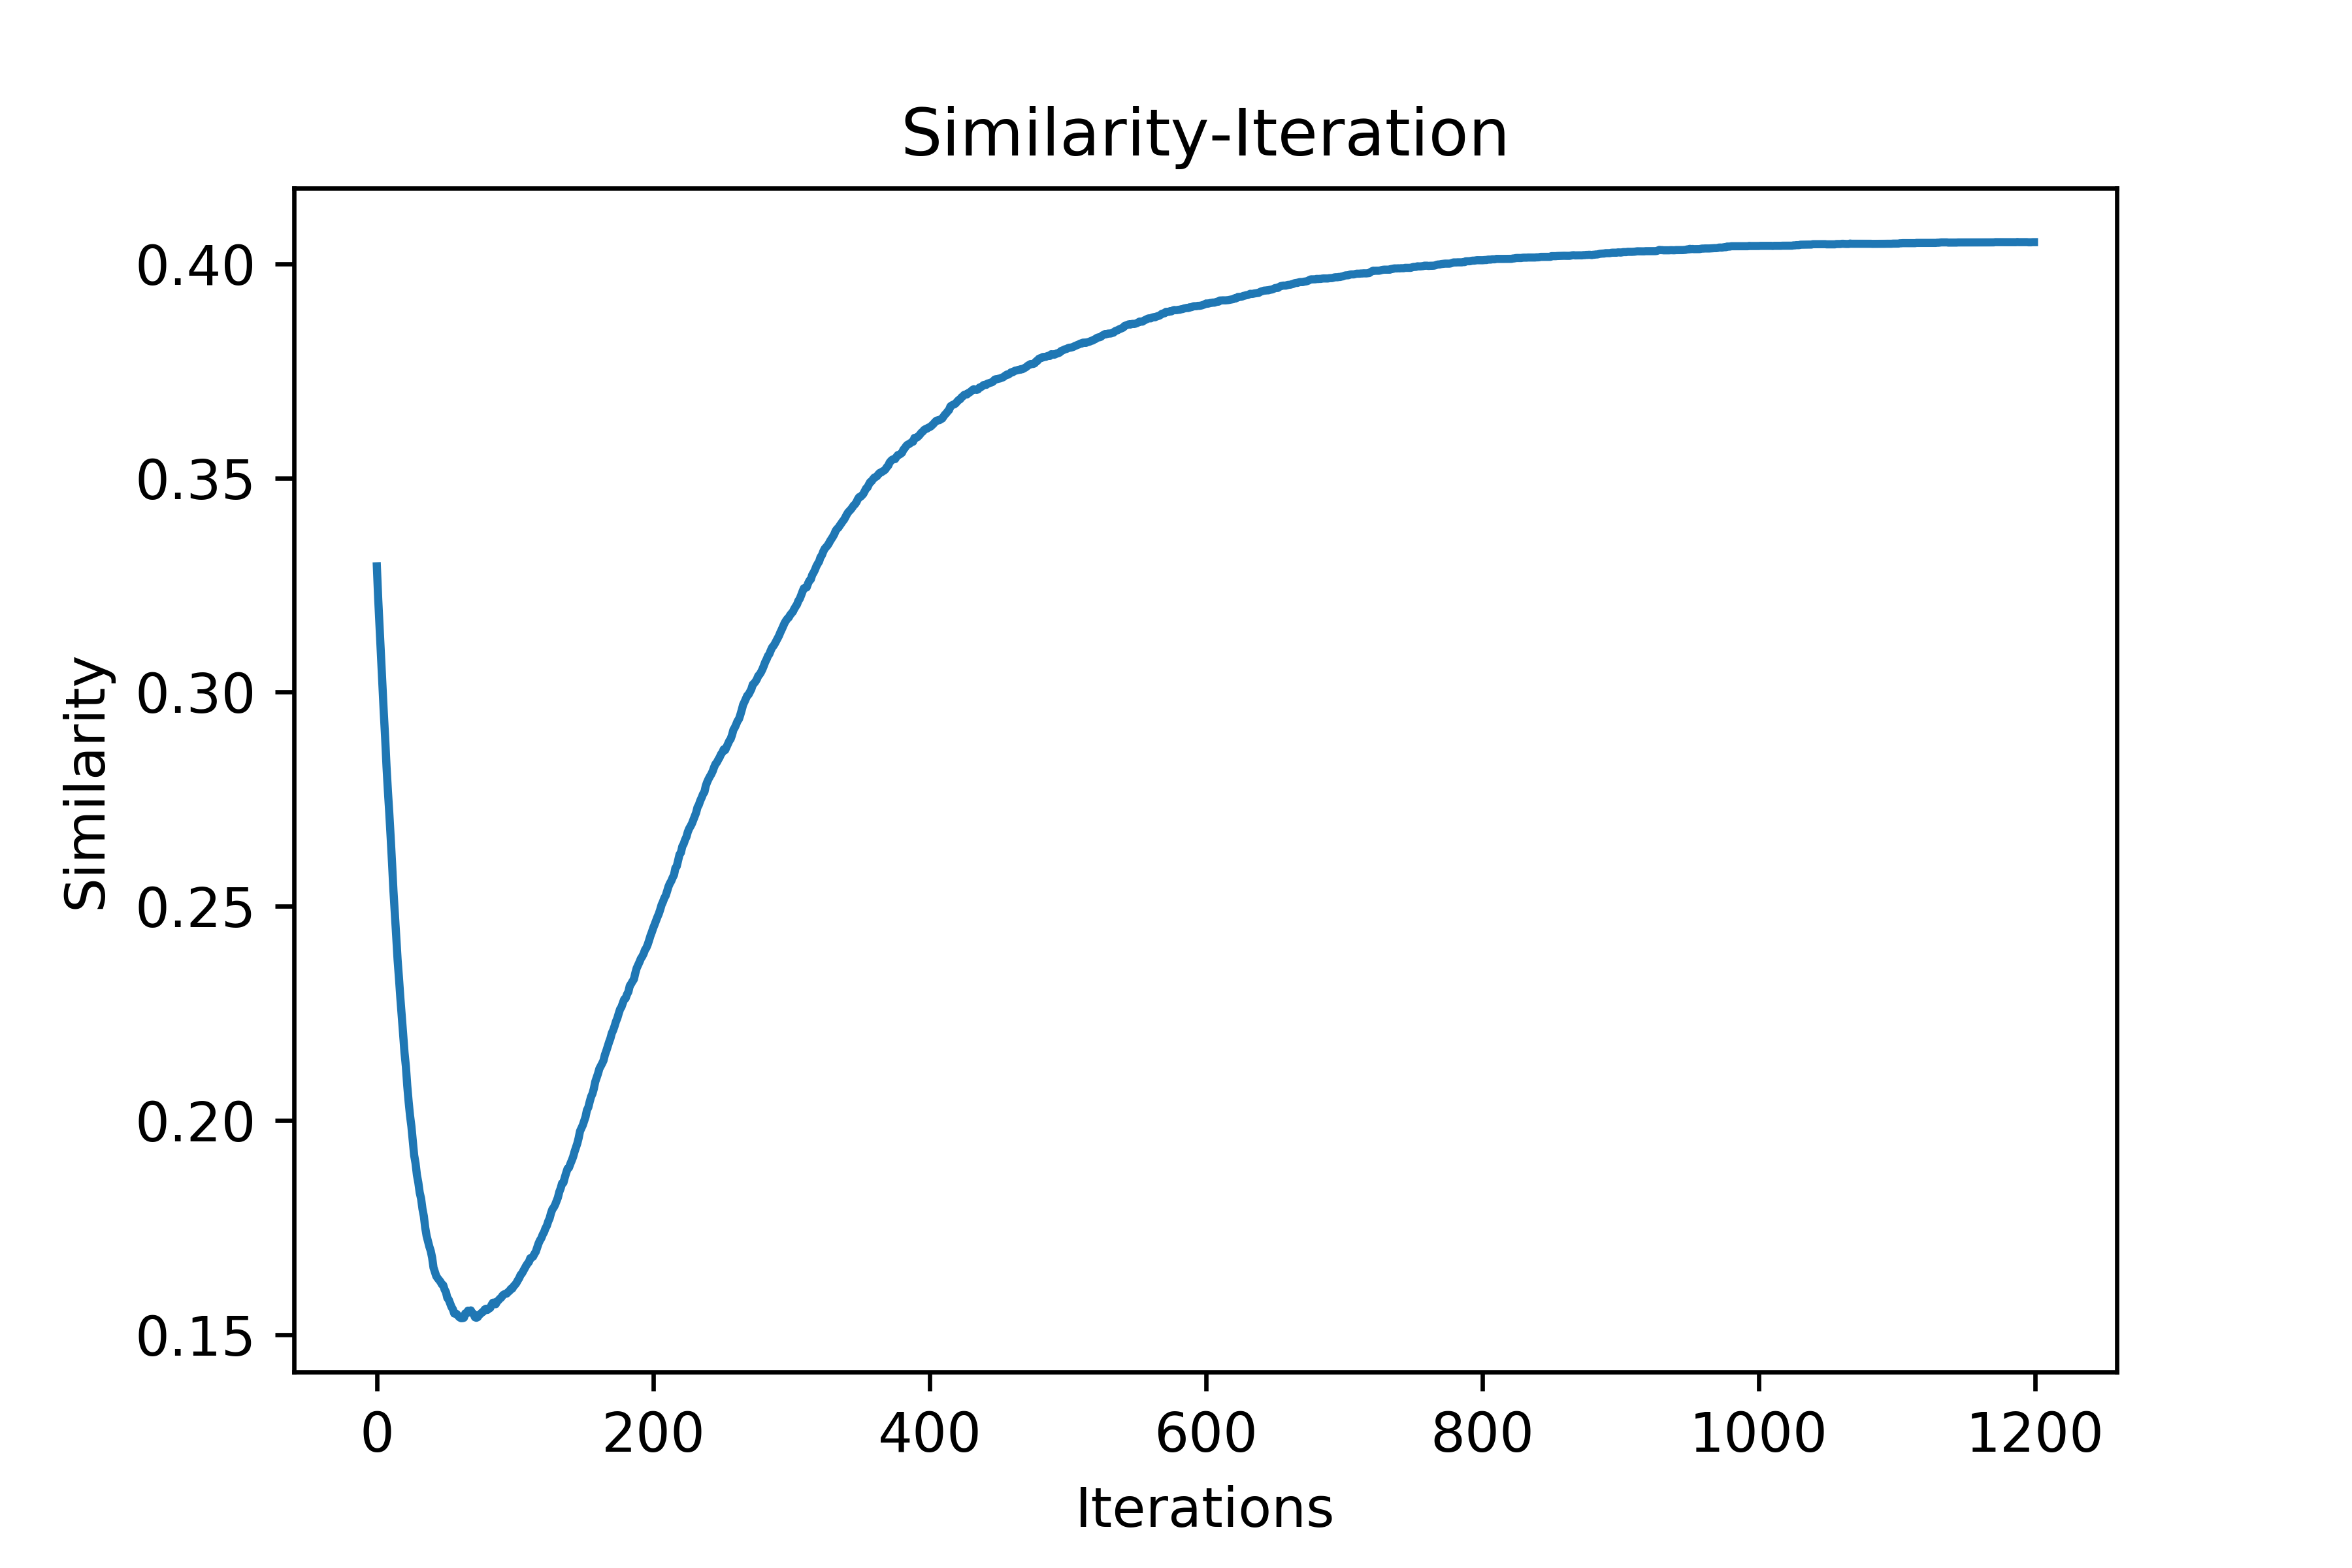
\includegraphics[width=0.9\textwidth]{Sim50_5_1200_100_3}
    	\caption{Similarity}\label{Sim50_5_1200_100_3_h}
    \end{figure}
    %
    \begin{figure}[H]
    	\centering
    	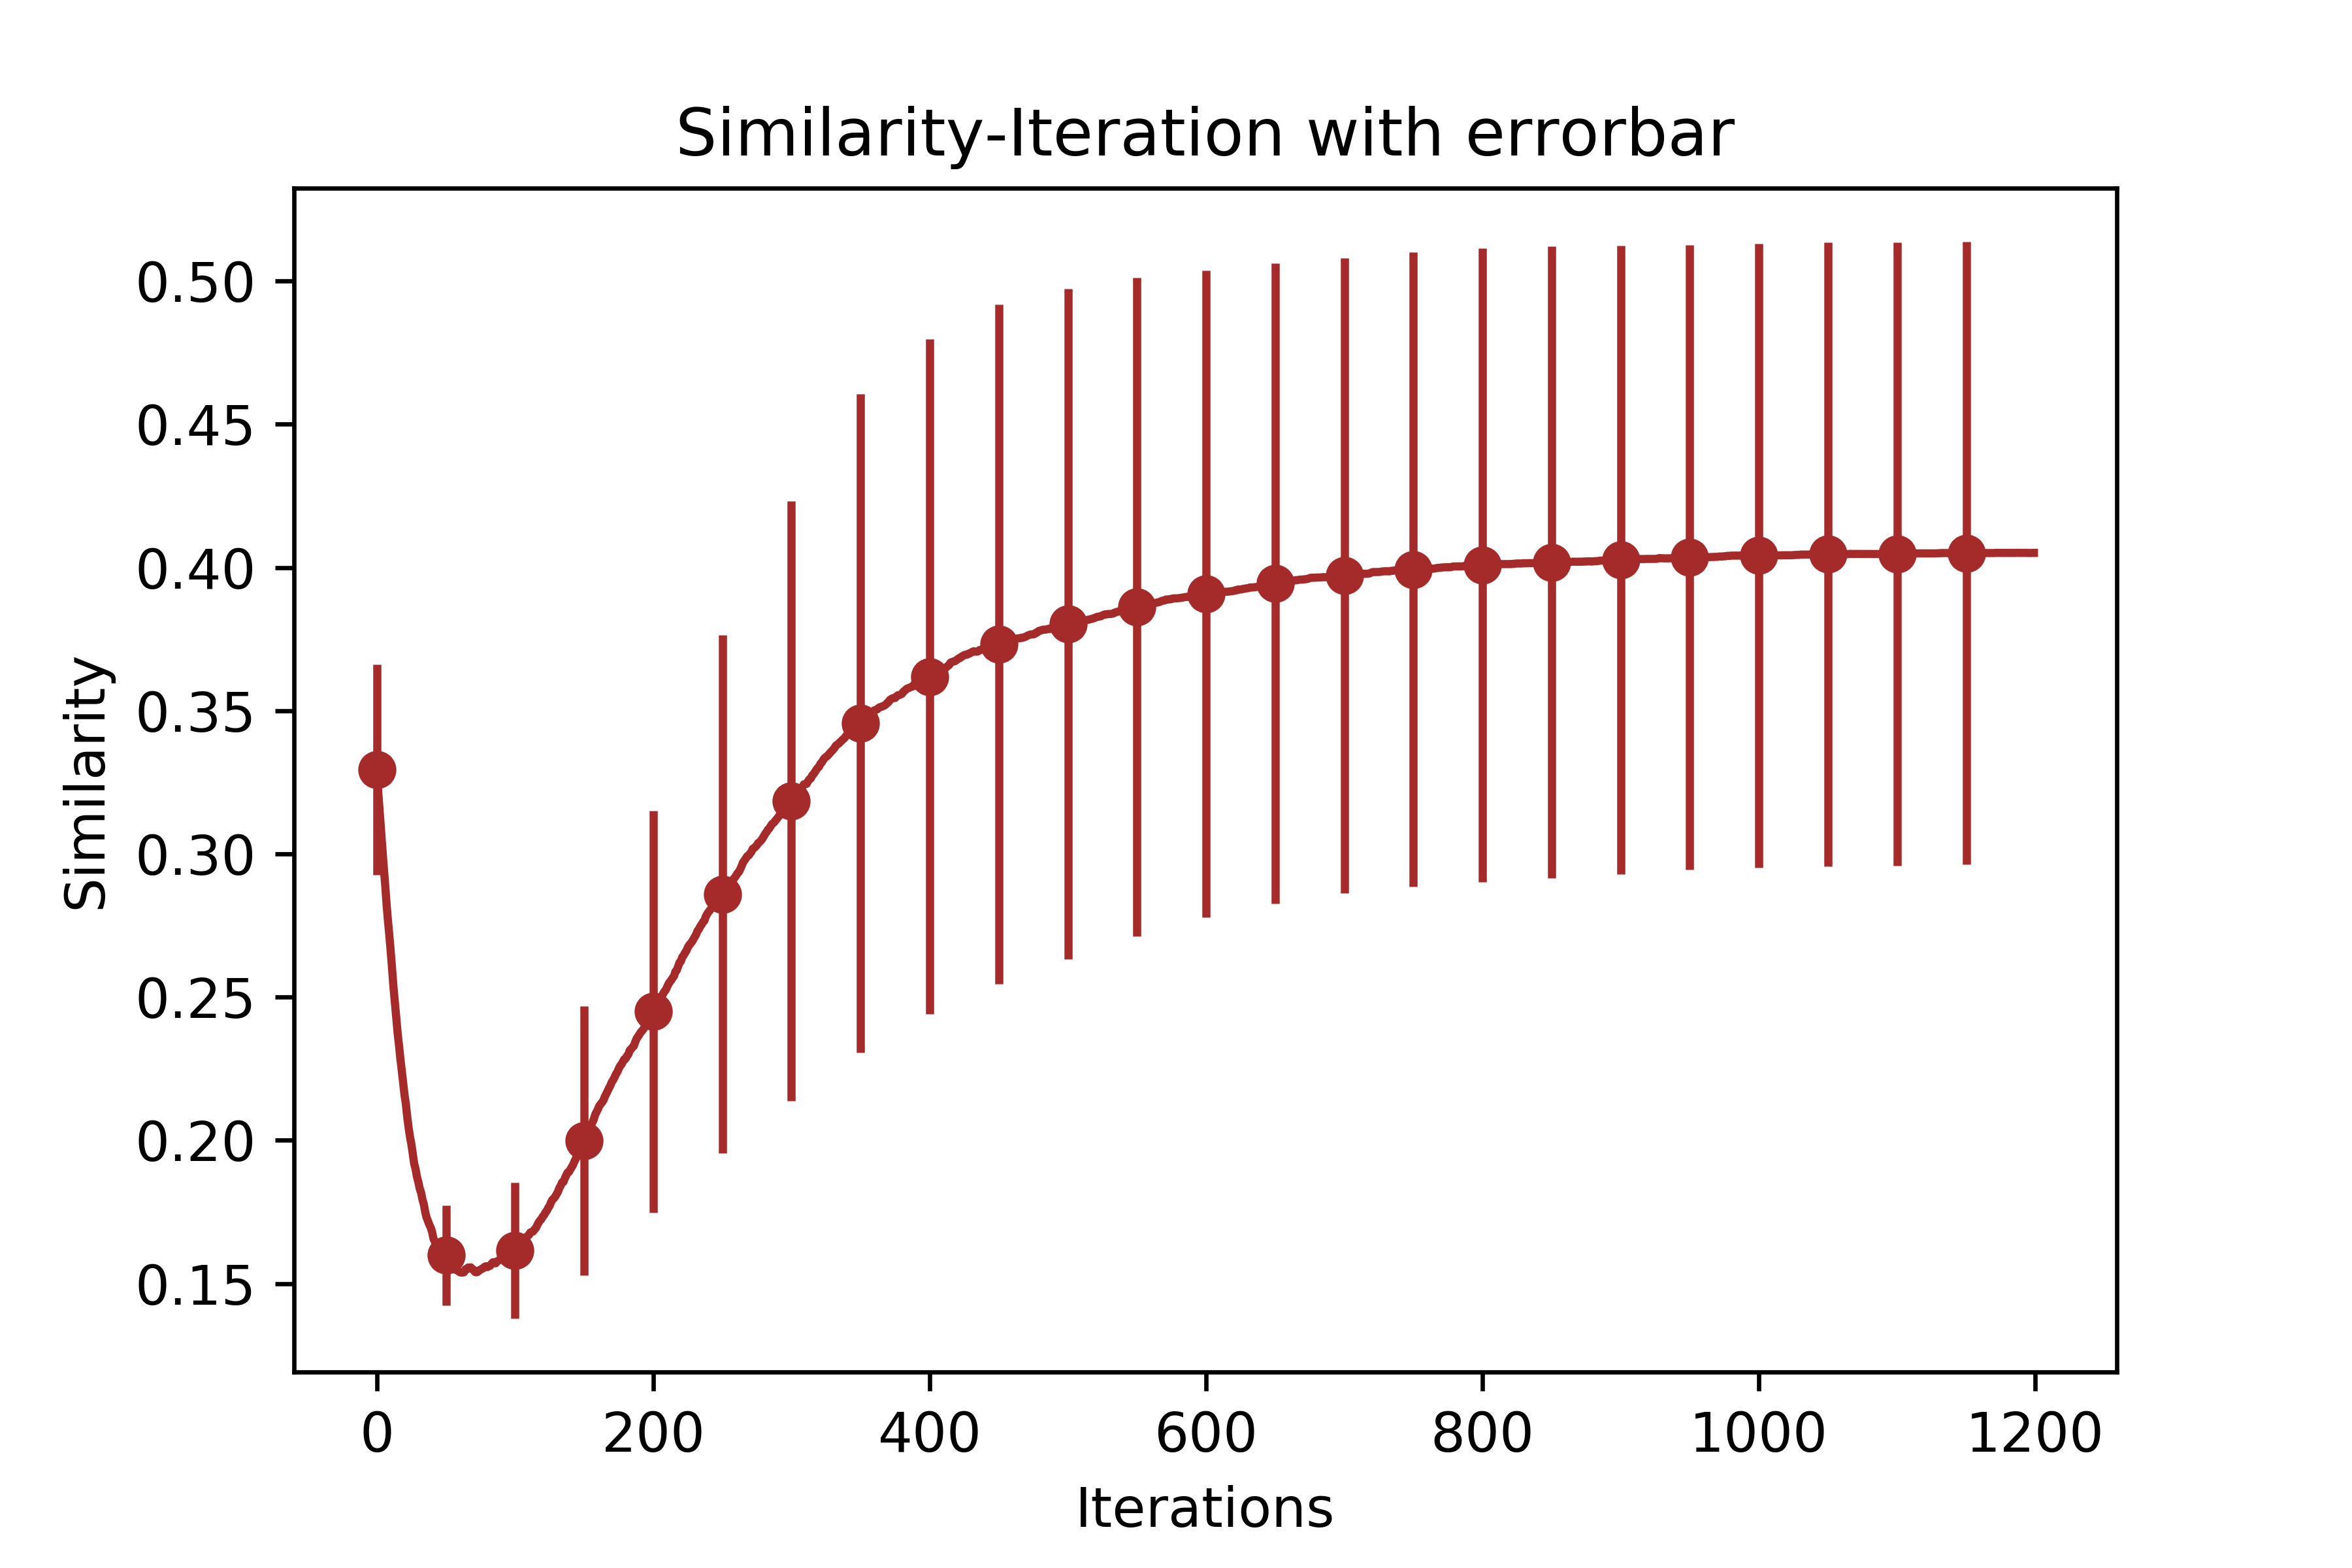
\includegraphics[width=0.9\textwidth]{SimErr50_5_1200_100_3}
    	\caption{Similarity with error bar}\label{SimErr50_5_1200_100_3_h}
    \end{figure}
    %
    \begin{figure}[H]
    	\centering
    	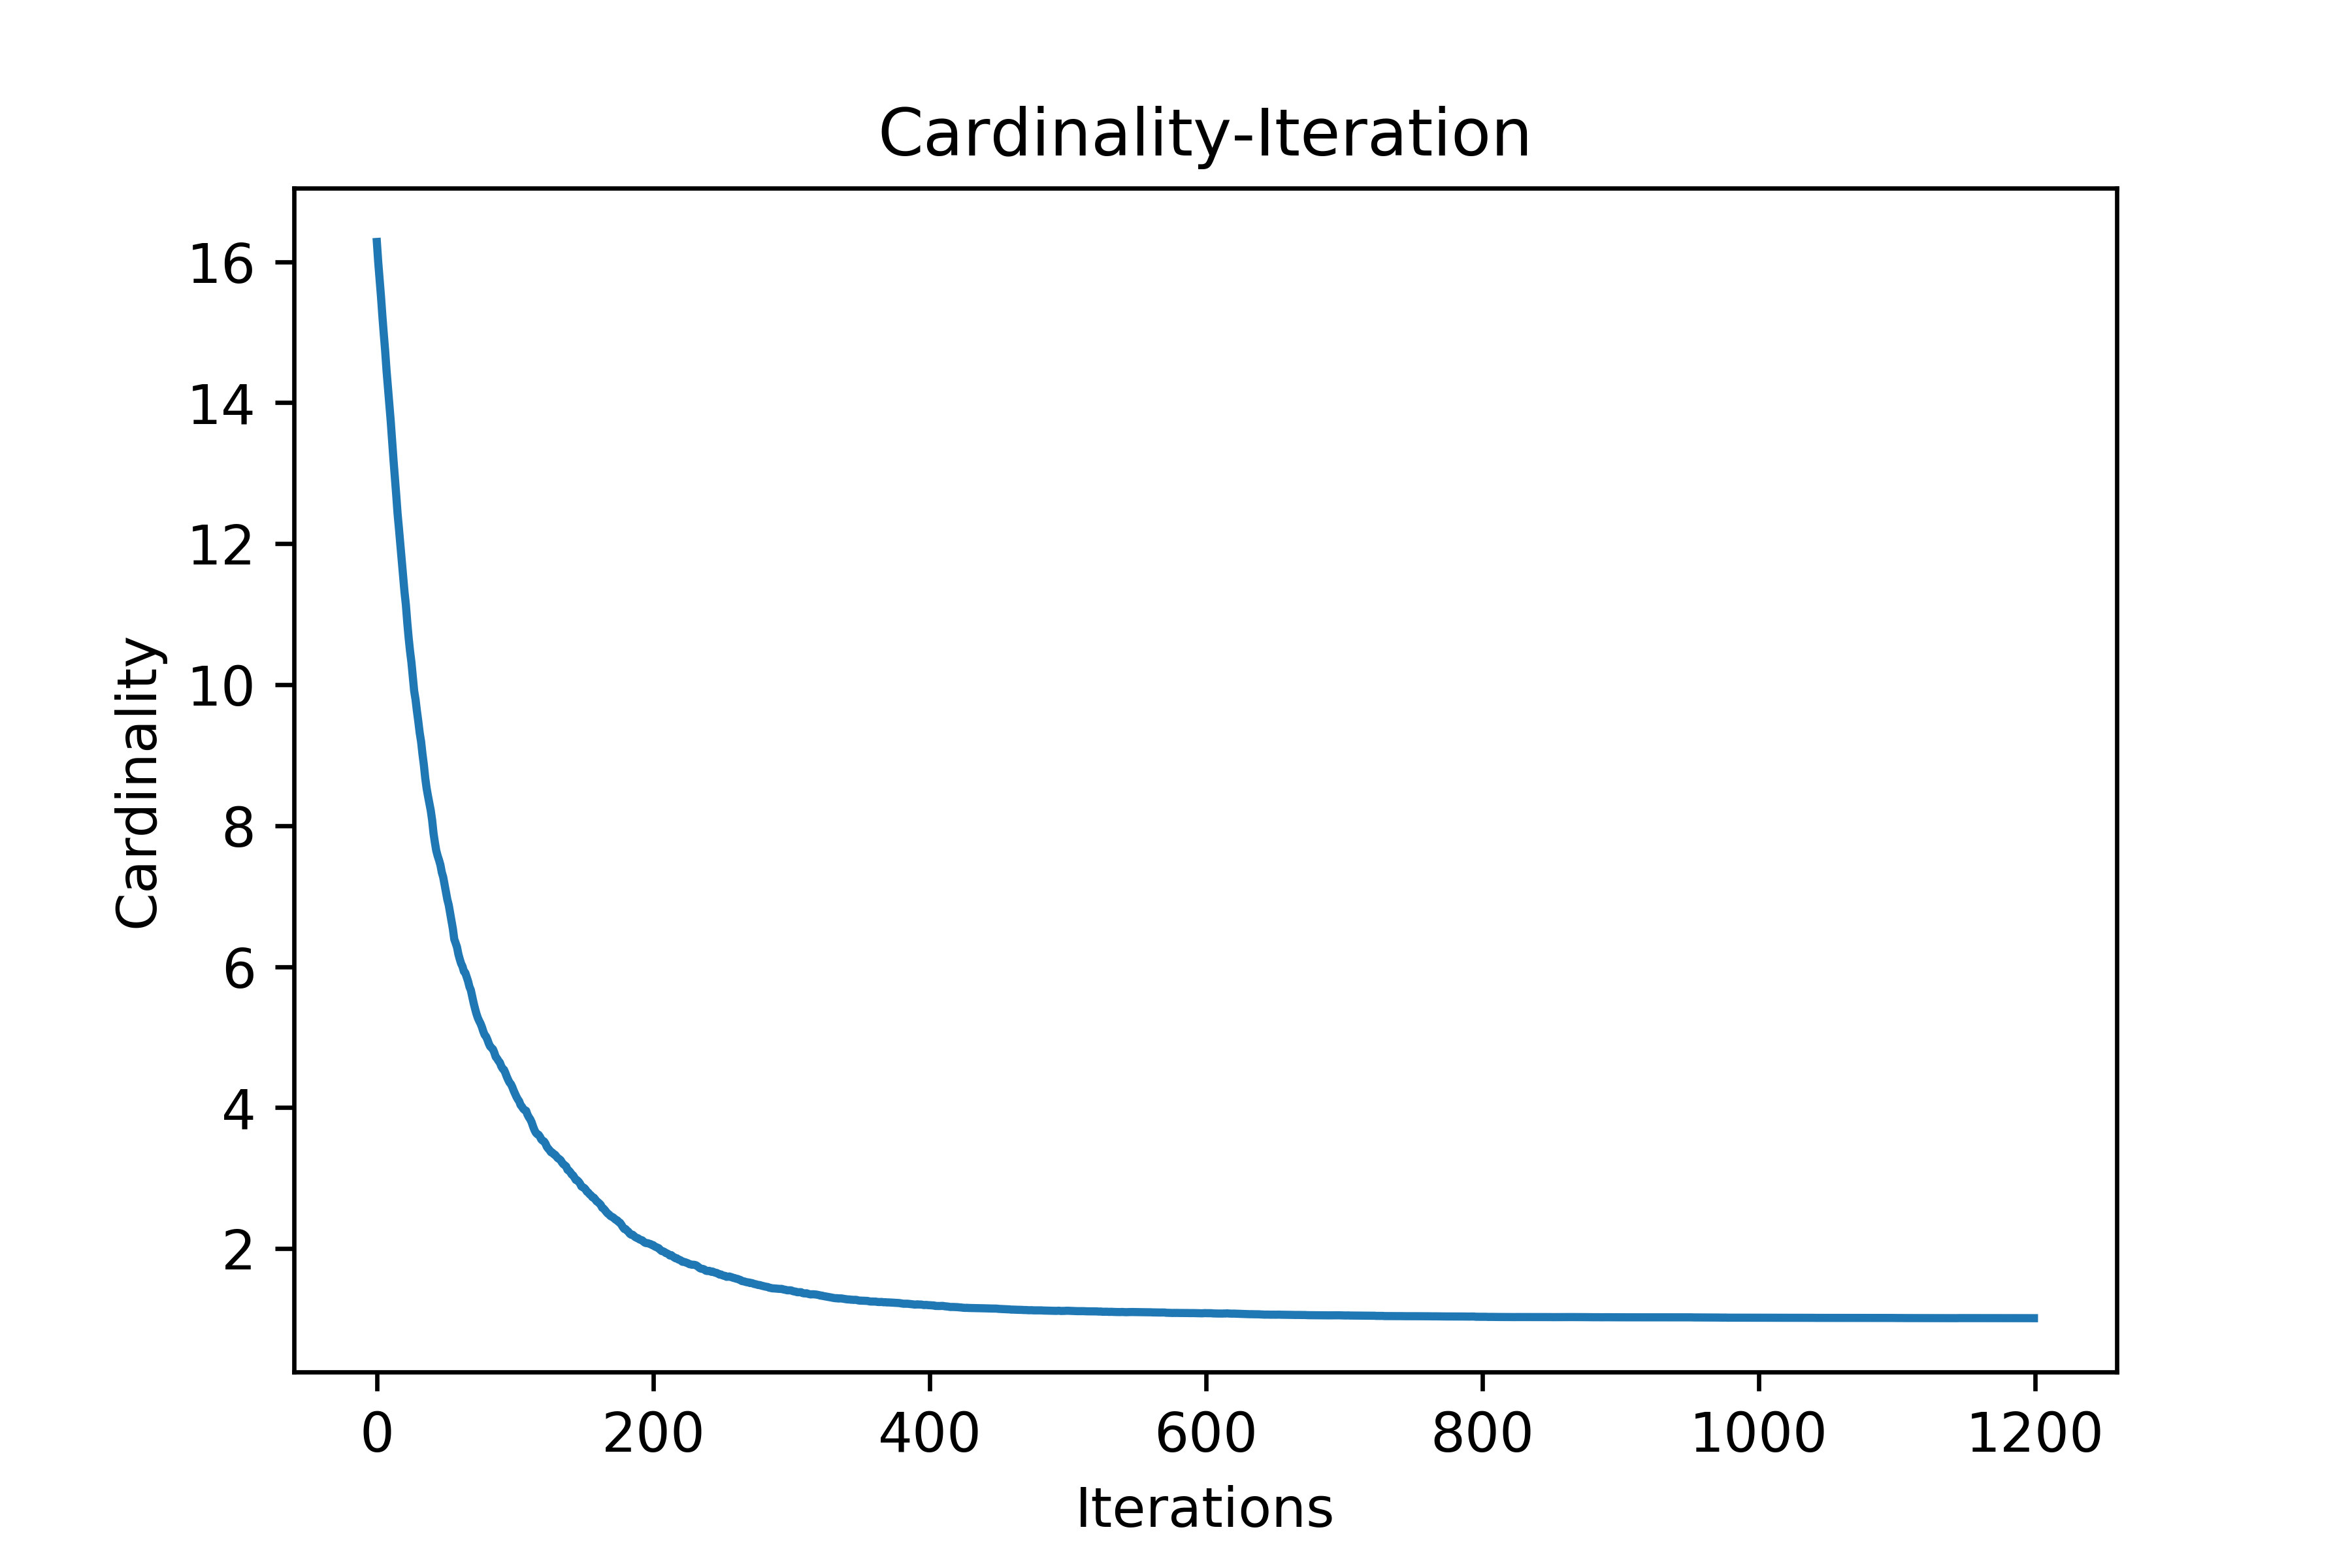
\includegraphics[width=0.9\textwidth]{Card50_5_1200_100_3}
    	\caption{Cardinality}\label{Card50_5_1200_100_3_h}
    \end{figure}
    %
    \begin{figure}[H]
    	\centering
    	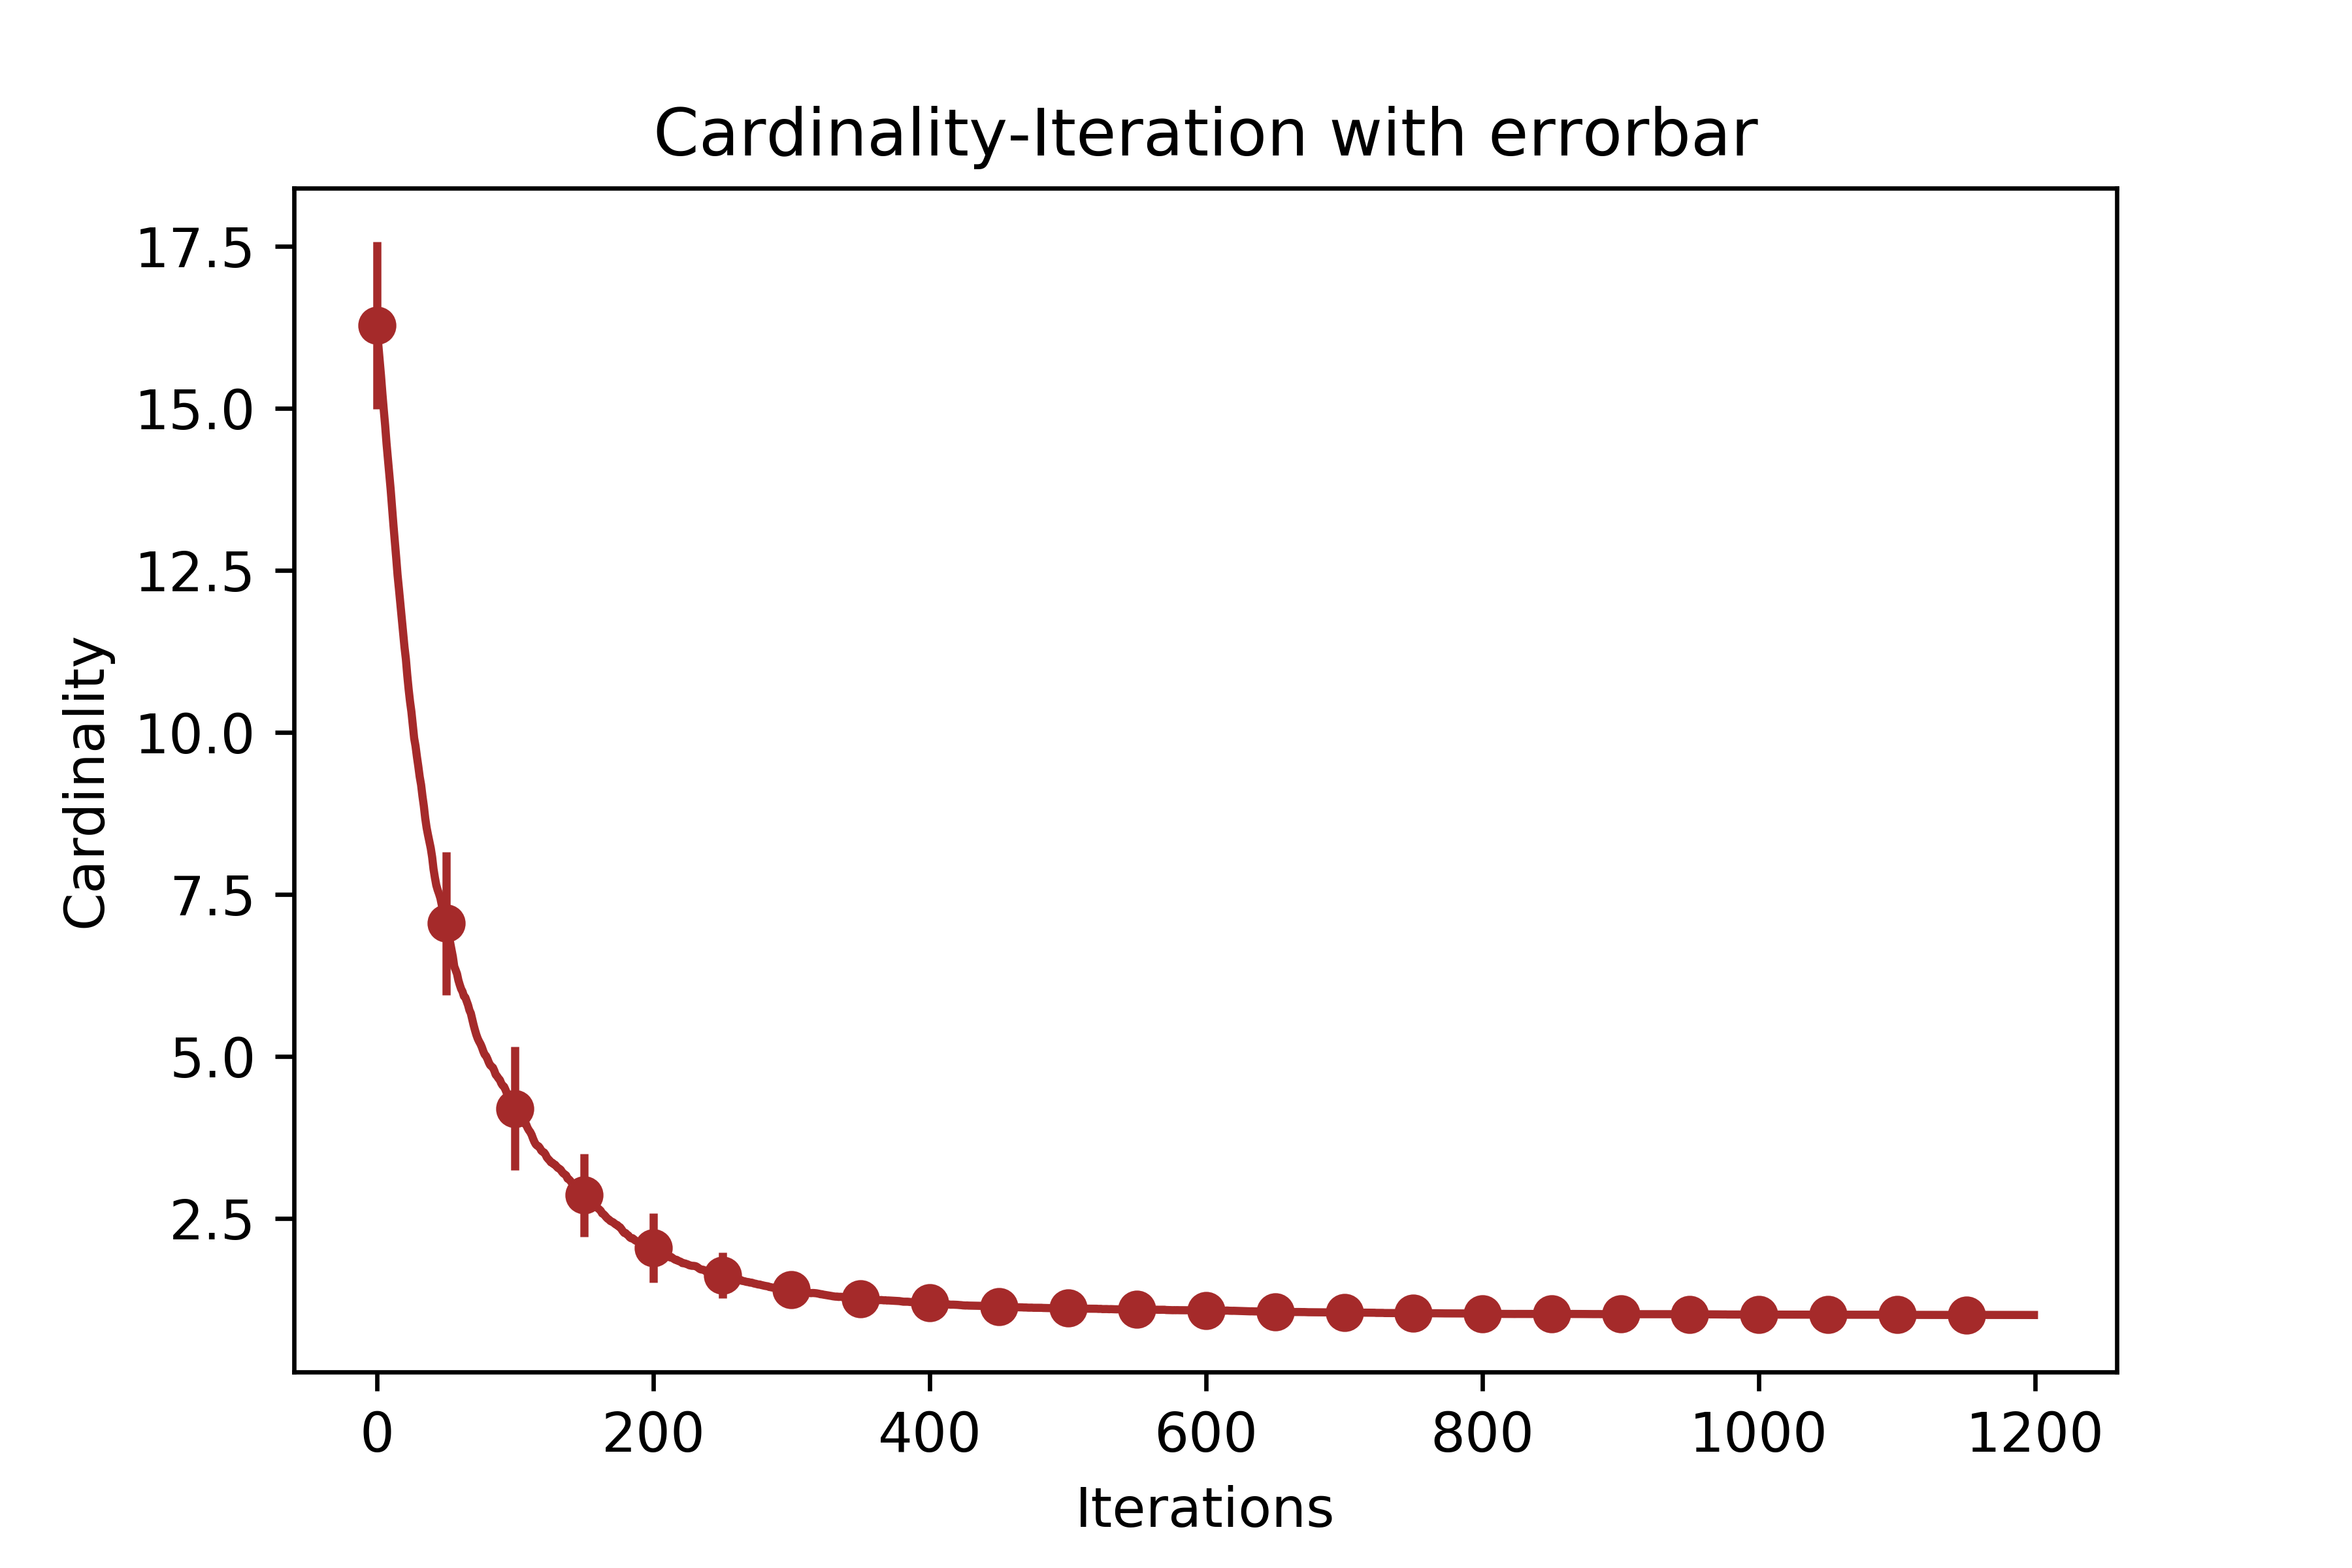
\includegraphics[width=0.9\textwidth]{CardErr50_5_1200_100_3}
    	\caption{Cardinality with error bar}\label{CardErr50_5_1200_100_3_h}
    \end{figure}
    \begin{figure}[H]
    	\centering
    	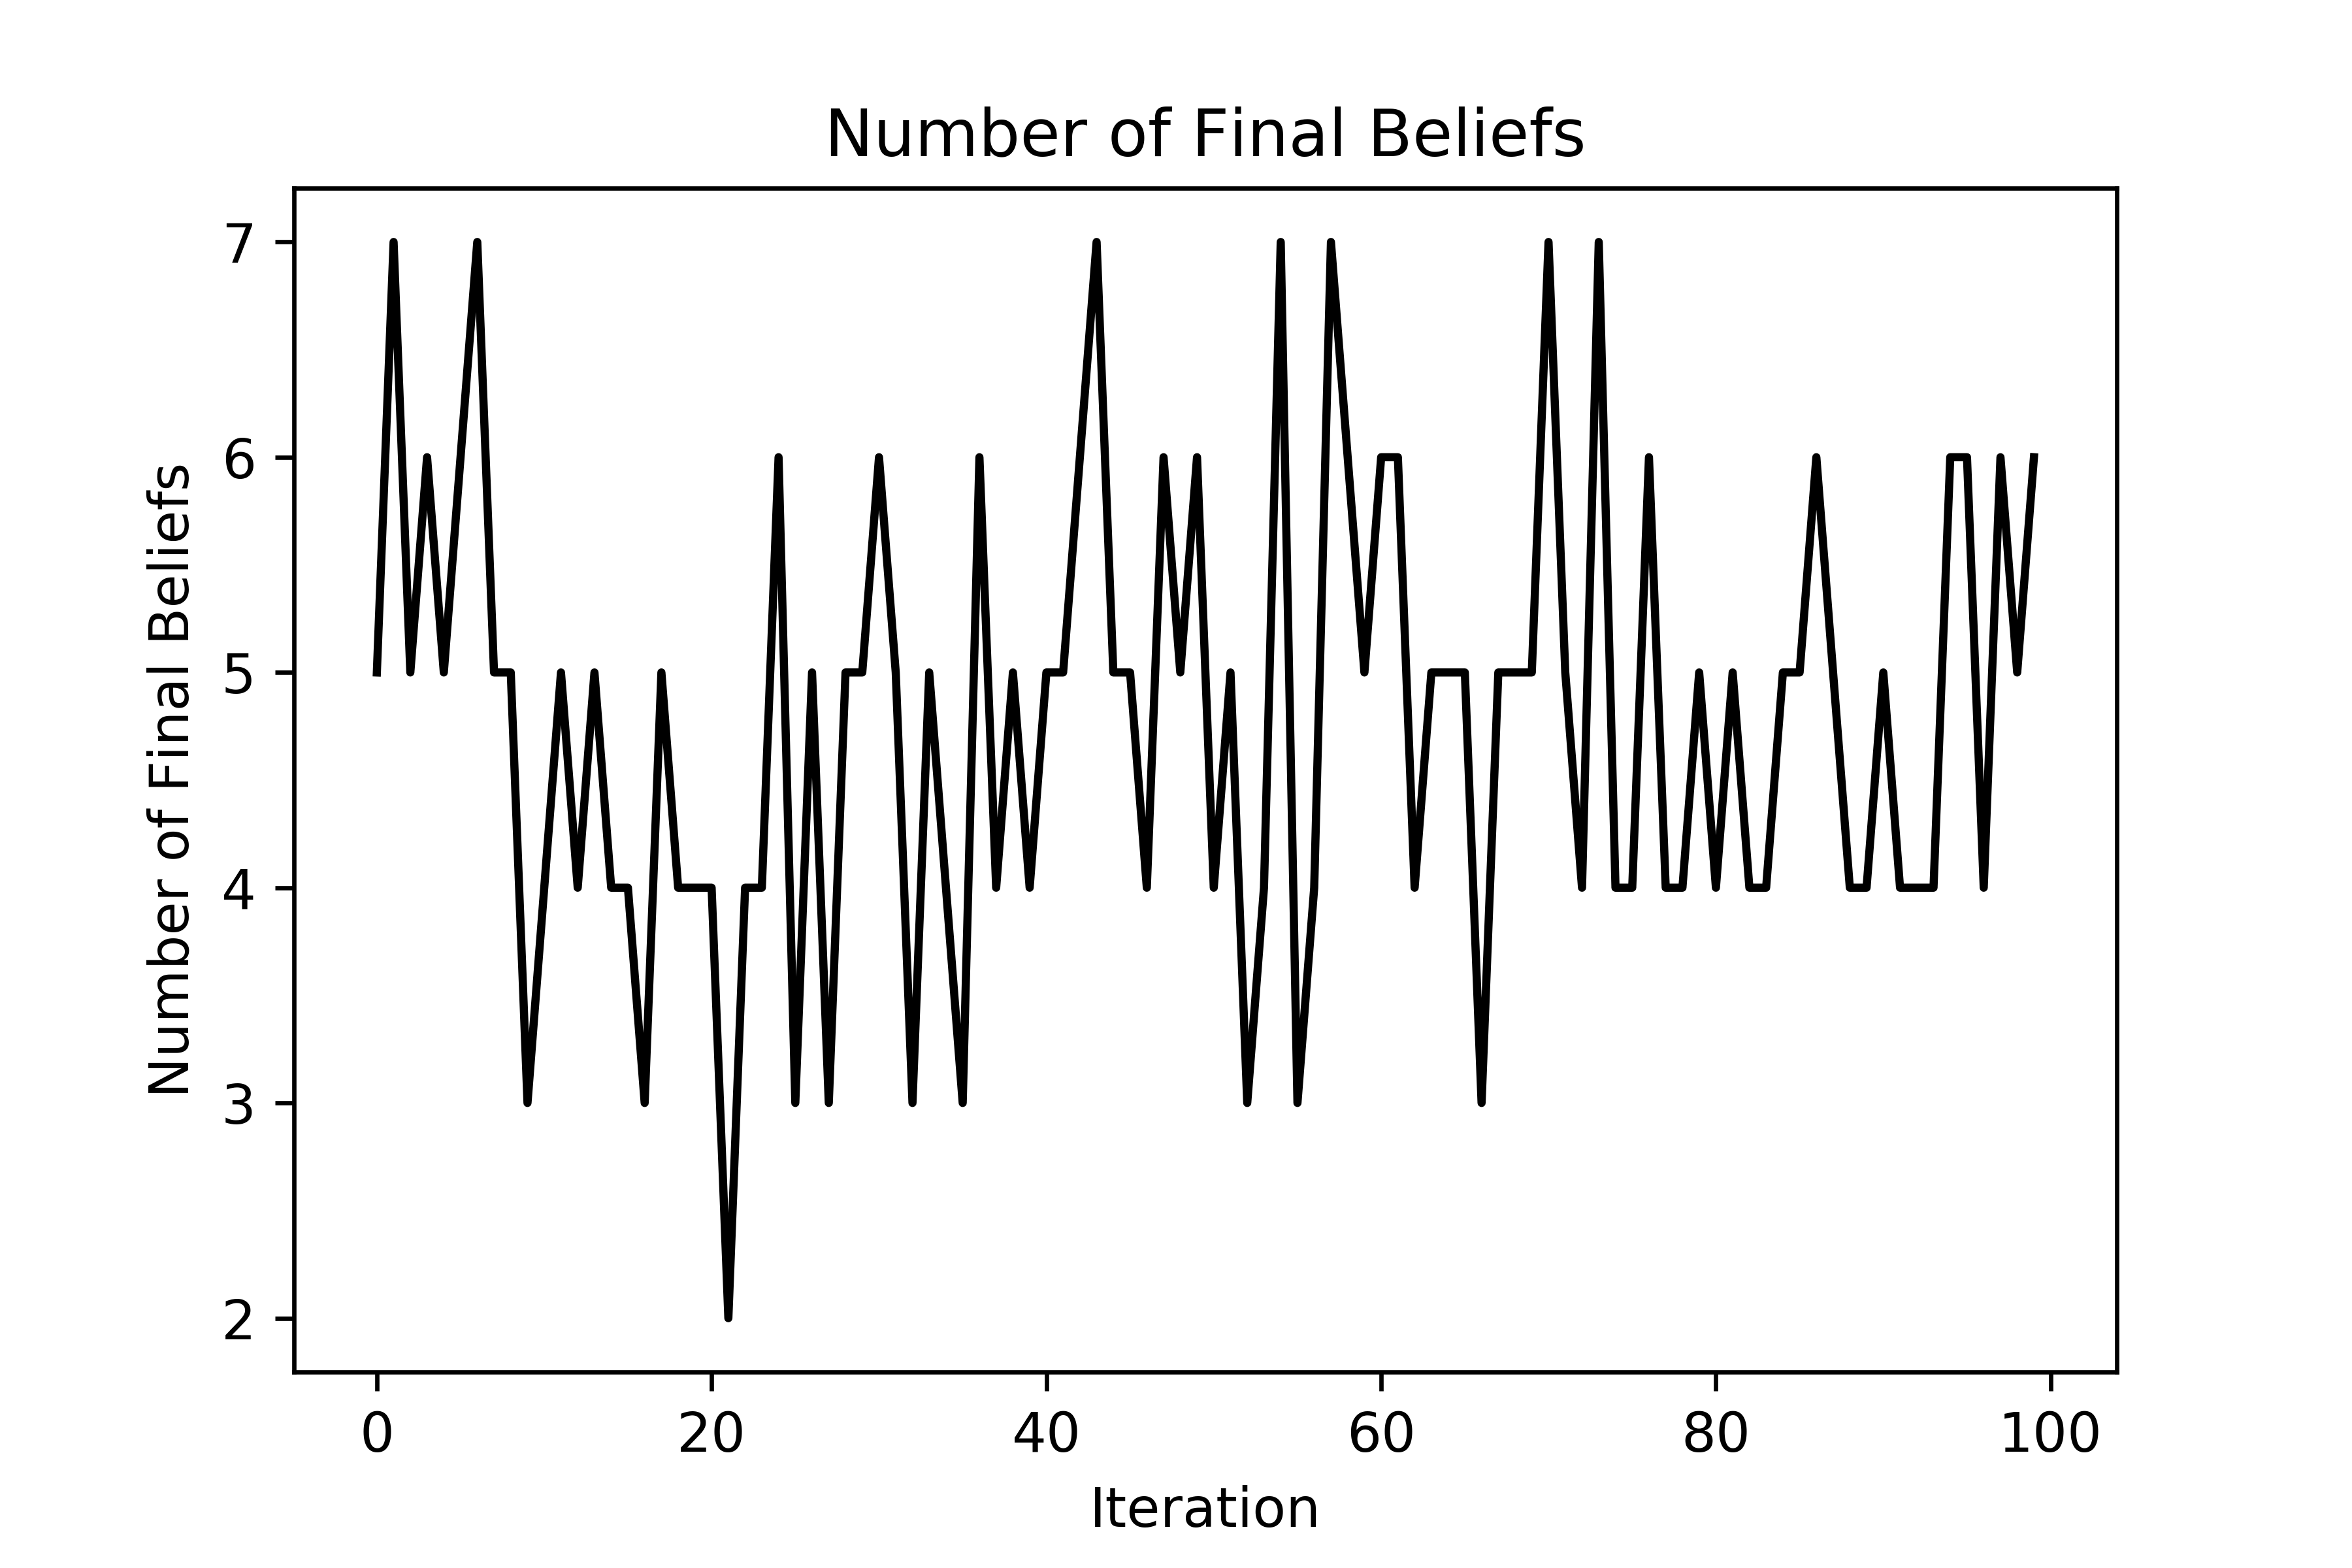
\includegraphics[width=0.9\textwidth]{numbef50_5_1200_100_3}
    	\caption{Cardinality with error bar}\label{numbef50_5_1200_100_3}
    \end{figure}
%%
        \subsection{50\_5\_1200\_100\_0.5}
    Time used: 104.99307195062624${s}$
    \begin{figure}[H]
    	\centering
    	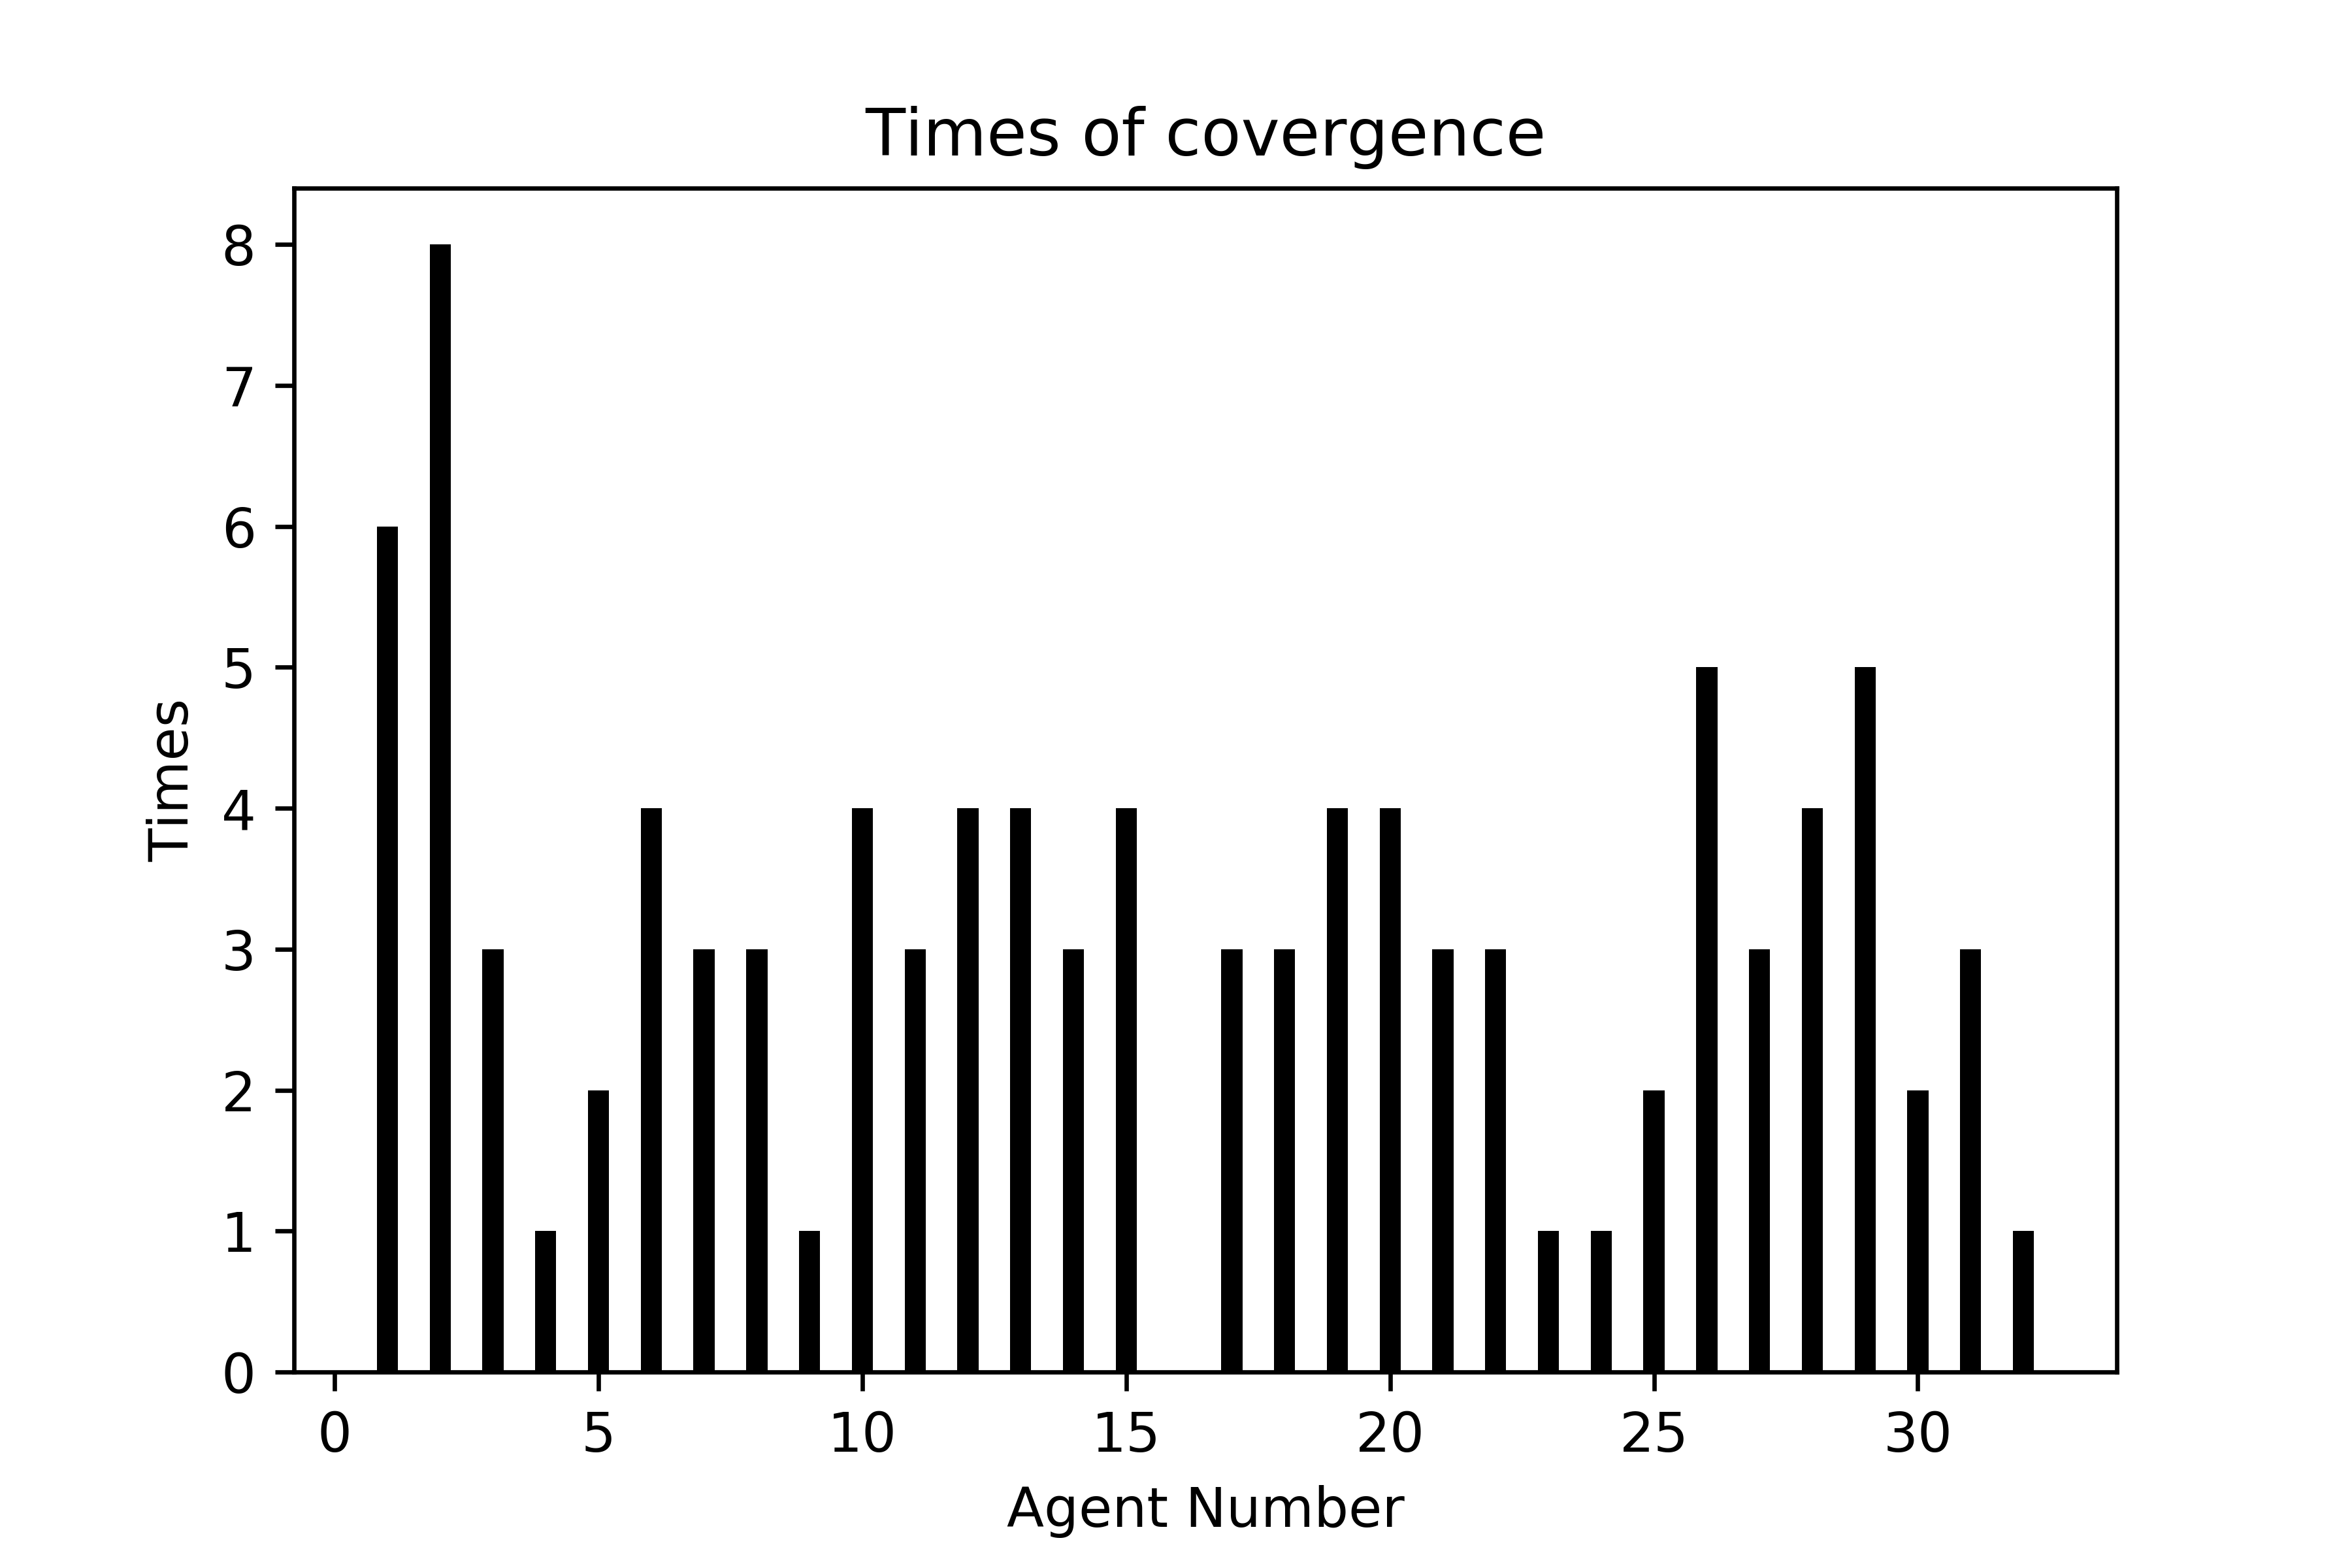
\includegraphics[width=0.9\textwidth]{agt50_5_1200_1000_5.png}
    	\caption{Where the iterations converge}\label{agt50_5_1200_1000.5_h}
    \end{figure}
    %
    \begin{figure}[H]
    	\centering
    	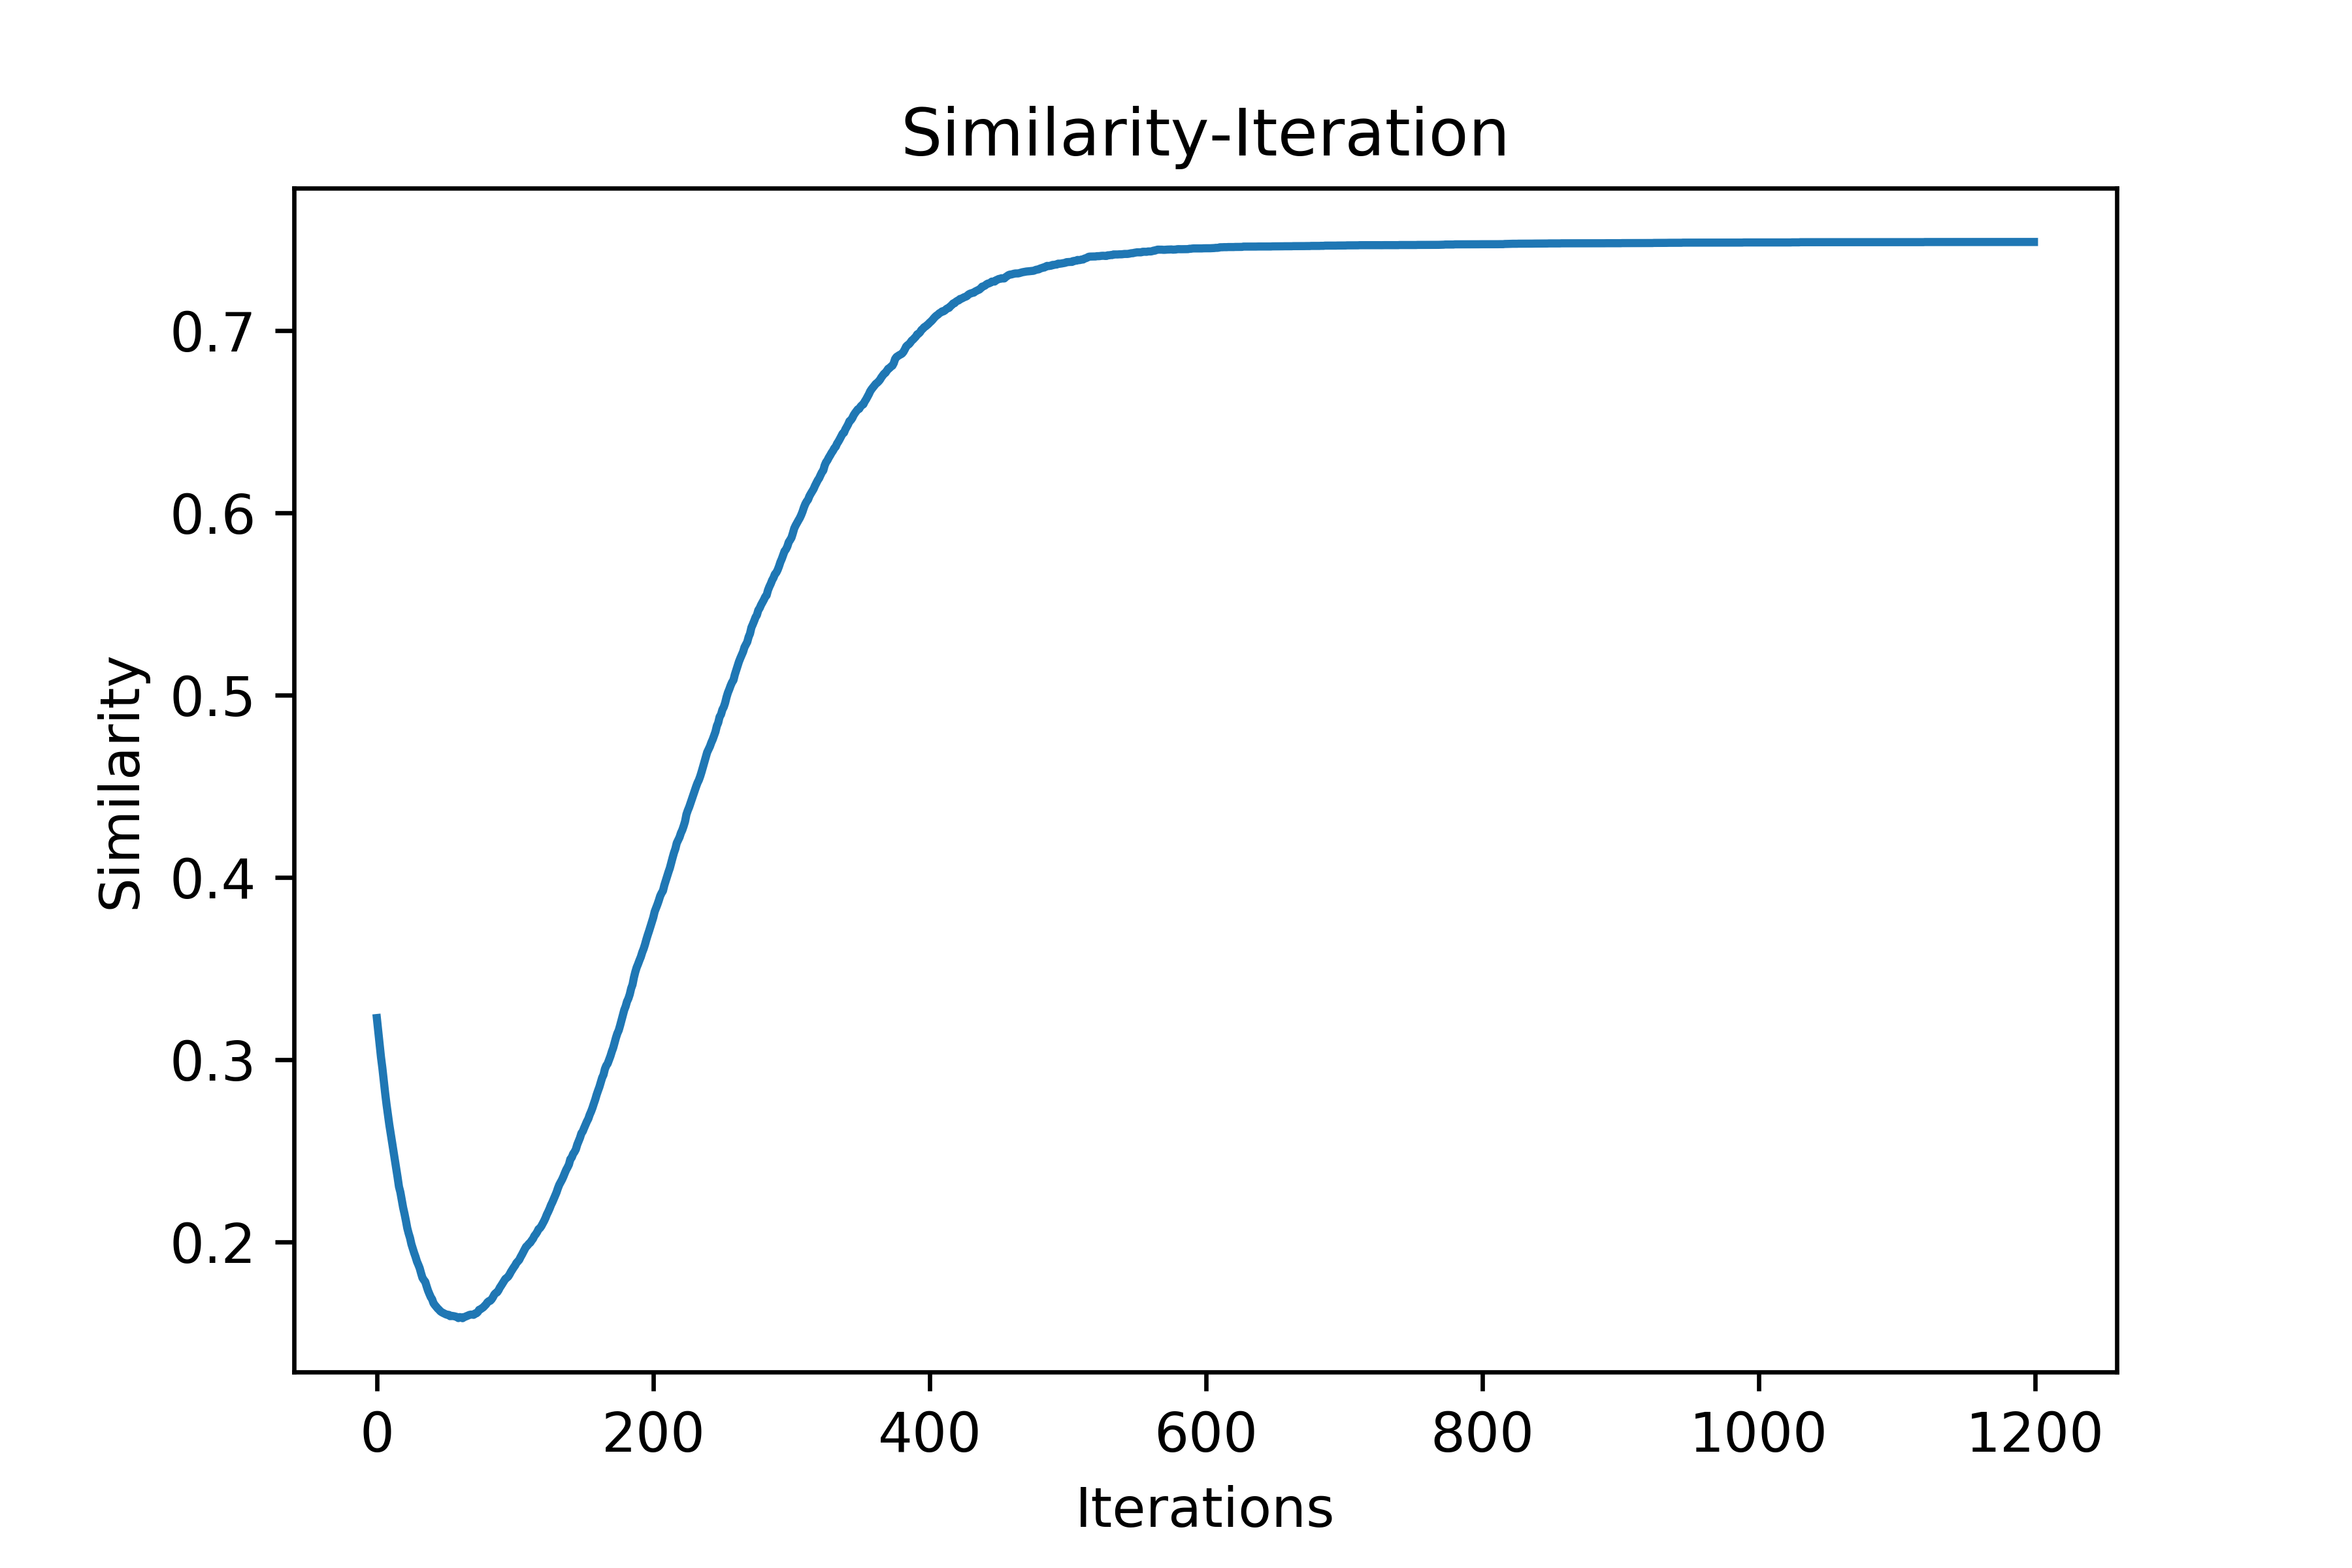
\includegraphics[width=0.9\textwidth]{Sim50_5_1200_1000_5}
    	\caption{Similarity}\label{Sim50_5_1200_1000.5_h}
    \end{figure}
    %
    \begin{figure}[H]
    	\centering
    	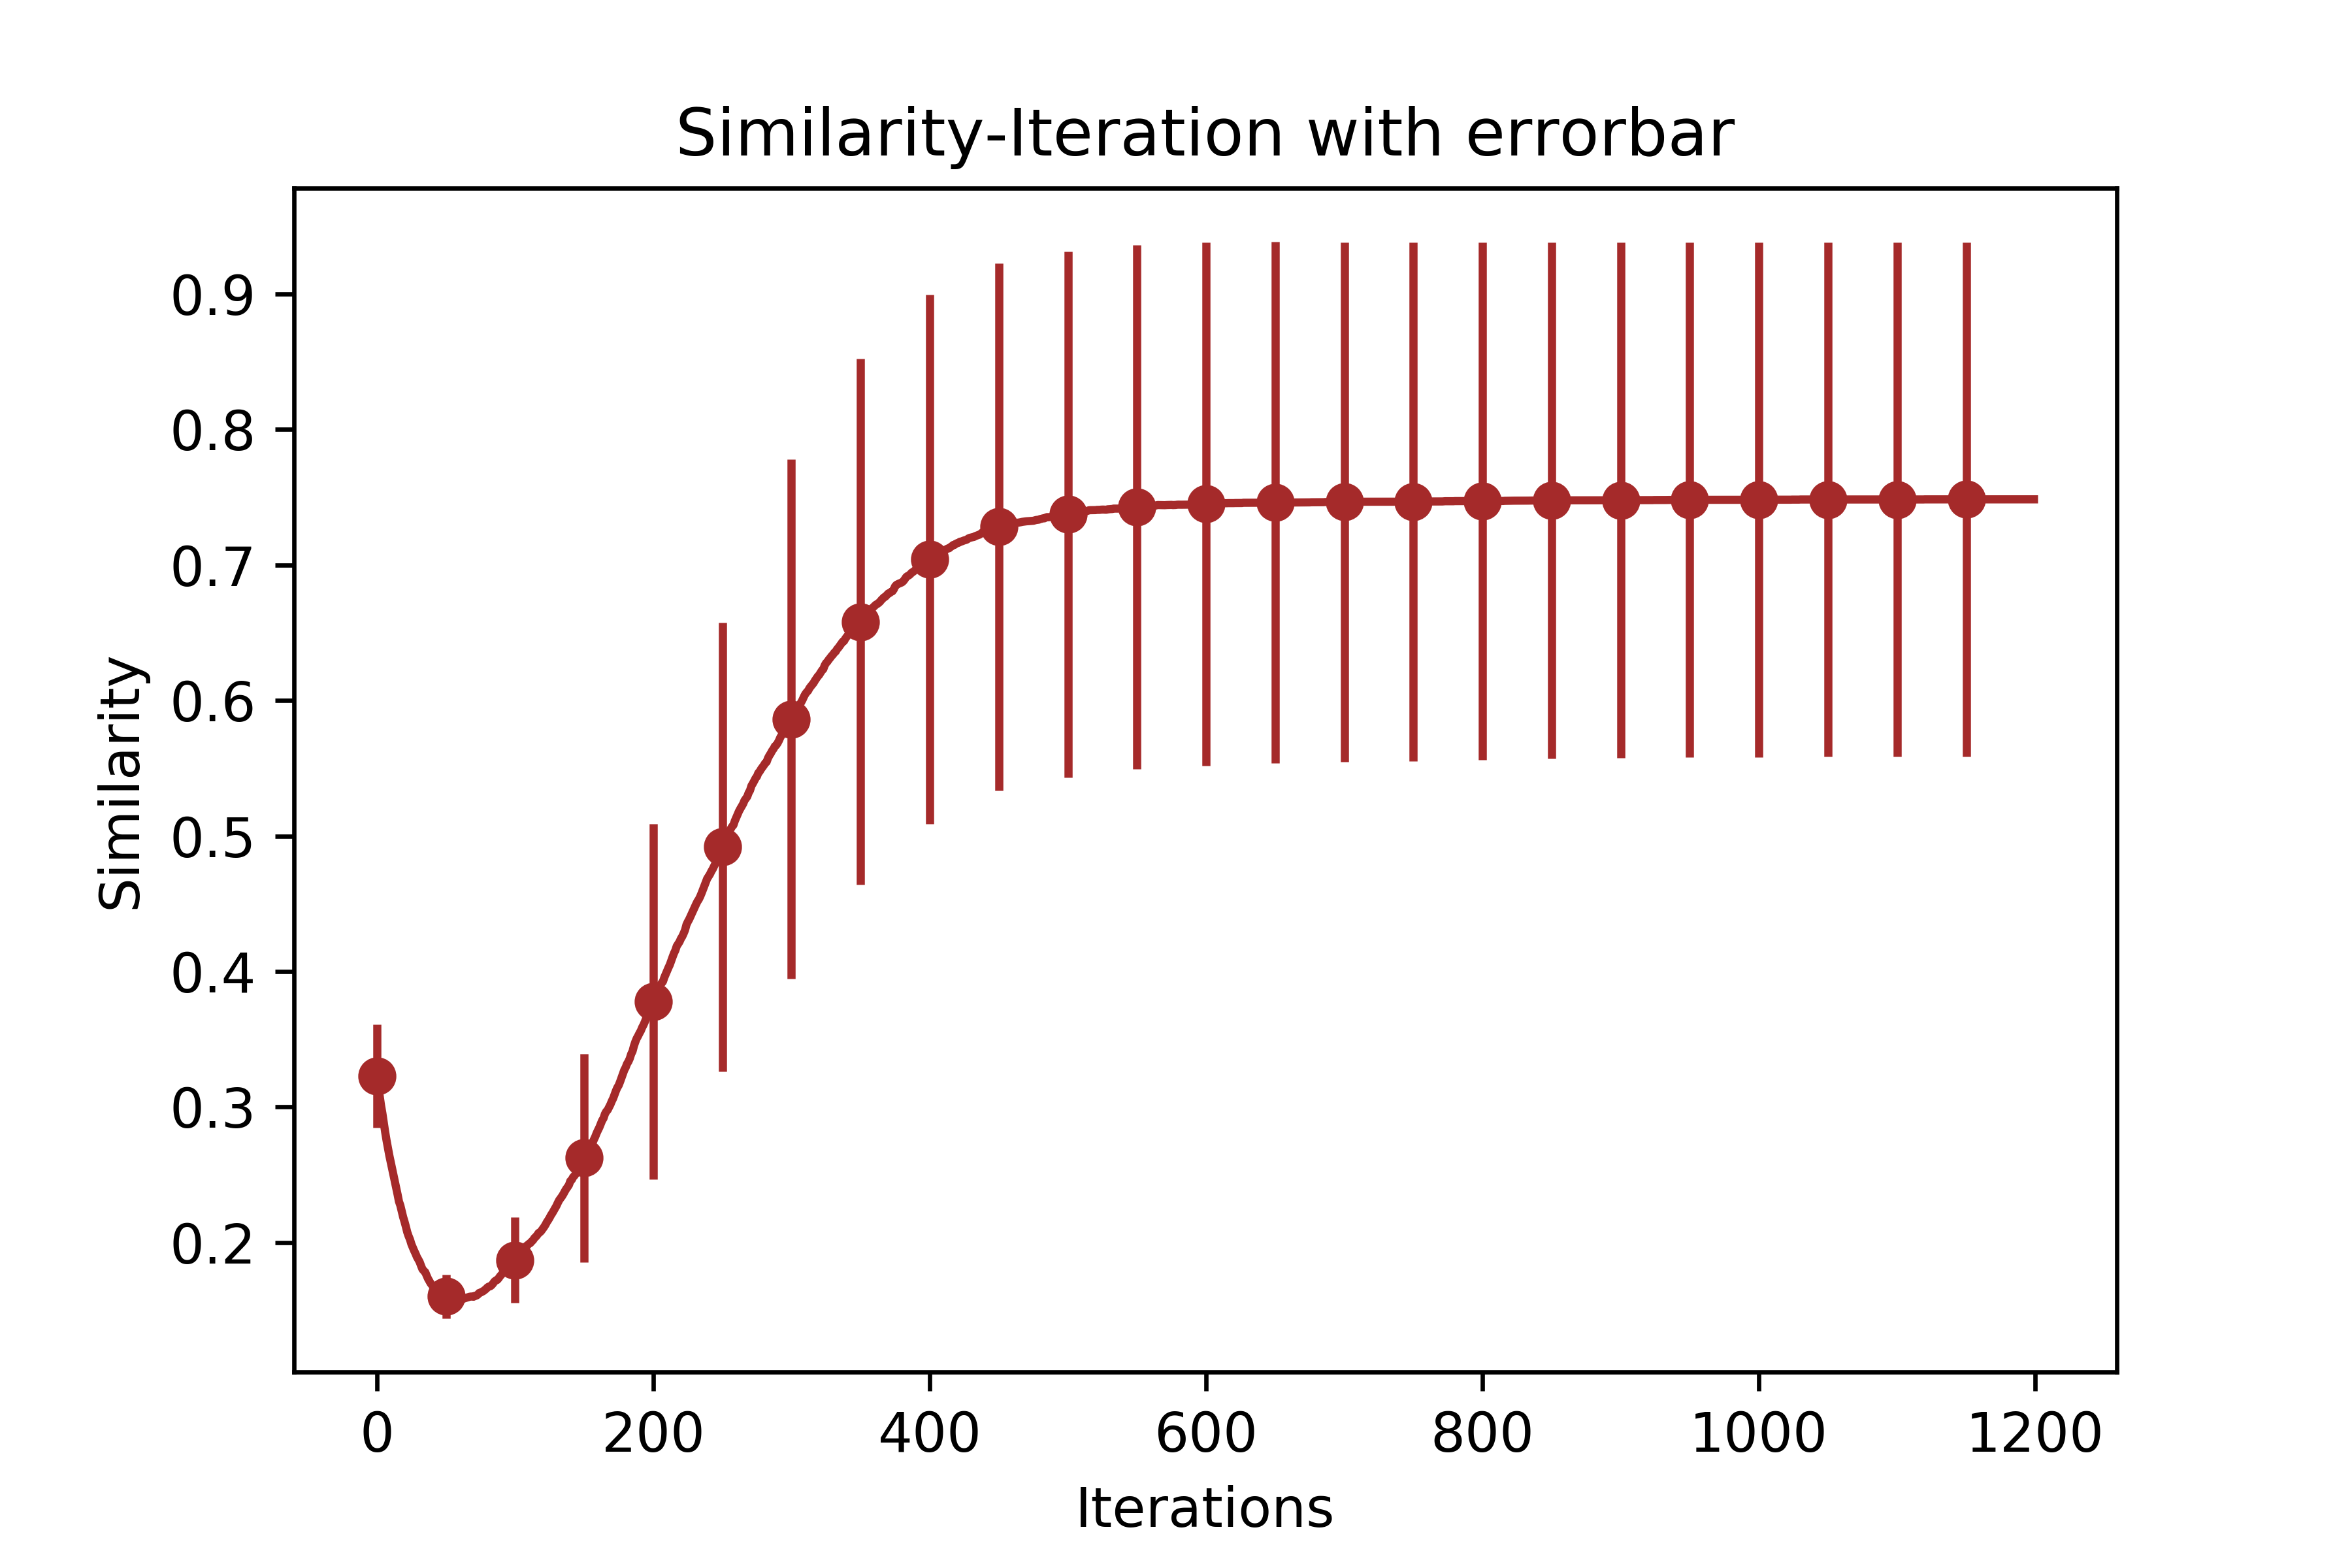
\includegraphics[width=0.9\textwidth]{SimErr50_5_1200_1000_5}
    	\caption{Similarity with error bar}\label{SimErr50_5_1200_1000.5_h}
    \end{figure}
    %
    \begin{figure}[H]
    	\centering
    	\includegraphics[width=0.9\textwidth]{Card50_5_1200_1000_5}
    	\caption{Cardinality}\label{Card50_5_1200_1000.5_h}
    \end{figure}
    %
    \begin{figure}[H]
    	\centering
    	\includegraphics[width=0.9\textwidth]{CardErr50_5_1200_1000_5}
    	\caption{Cardinality with error bar}\label{CardErr50_5_1200_1000.5_h}
    \end{figure}
    \begin{figure}[H]
    	\centering
    	\includegraphics[width=0.9\textwidth]{numbef50_5_1200_1000_5}
    	\caption{Cardinality with error bar}\label{numbef50_5_1200_1000.5}
    \end{figure}
    %%
    \subsection{100\_4\_1500\_100\_0.5}
    Time used: 547.3942672014223${s}$
    \begin{figure}[H]
    	\centering
    	\includegraphics[width=0.9\textwidth]{agt100_4_1500_100_5}
    	\caption{Where the iterations converge}\label{agt100_4_1500_100_5_h}
    \end{figure}
    %
    \begin{figure}[H]
    	\centering
    	\includegraphics[width=0.9\textwidth]{Sim100_4_1500_100_5}
    	\caption{Similarity}\label{Sim100_4_1500_100_5_h}
    \end{figure}
    %
    \begin{figure}[H]
    	\centering
    	\includegraphics[width=0.9\textwidth]{SimErr100_4_1500_100_5}
    	\caption{Similarity with error bar}\label{SimErr100_4_1500_100_5_h}
    \end{figure}
    %
    \begin{figure}[H]
    	\centering
    	\includegraphics[width=0.9\textwidth]{Card100_4_1500_100_5}
    	\caption{Cardinality}\label{Card100_4_1500_100_5_h}
    \end{figure}
    %
    \begin{figure}[H]
    	\centering
    	\includegraphics[width=0.9\textwidth]{CardErr100_4_1500_100_5}
    	\caption{Cardinality with error bar}\label{CardErr100_4_1500_100_5_h}
    \end{figure}
    \begin{figure}[H]
    	\centering
    	\includegraphics[width=0.9\textwidth]{numbef100_4_1500_100_5}
    	\caption{Cardinality with error bar}\label{numbef100_4_1500_100_5}
    \end{figure}


%%Section min Hamming Distance
\section{Simulation Results with random initialise combine beliefs based on hamming distance(max)}\label{SRRImax}
the title: number of agents\_propositions\_iteration\_Times run\_threshold(Hamming distance)
\graphicspath{{figsMaxHamm/}}

\subsection{100\_4\_1500\_100\_0.5}
Time used: 113.40667891238468${s}$
\begin{figure}[H]
	\centering
	\includegraphics[width=0.9\textwidth]{agt50_4_1500_50_8}
	\caption{Where the iterations converge}\label{agt50_4_1500_100_8_mh}
\end{figure}
%
\begin{figure}[H]
	\centering
	\includegraphics[width=0.9\textwidth]{Sim50_4_1500_50_8}
	\caption{Similarity}\label{Sim50_4_1500_50_8_mh}
\end{figure}
%
\begin{figure}[H]
	\centering
	\includegraphics[width=0.9\textwidth]{SimErr50_4_1500_50_8}
	\caption{Similarity with error bar}\label{SimErr50_4_1500_50_8_mh}
\end{figure}
%
\begin{figure}[H]
	\centering
	\includegraphics[width=0.9\textwidth]{Card50_4_1500_50_8}
	\caption{Cardinality}\label{Card50_4_1500_50_8_mh}
\end{figure}
%
\begin{figure}[H]
	\centering
	\includegraphics[width=0.9\textwidth]{CardErr50_4_1500_50_8}
	\caption{Cardinality with error bar}\label{CardErr50_4_1500_50_8_mh}
\end{figure}
\begin{figure}[H]
	\centering
	\includegraphics[width=0.9\textwidth]{numbef50_4_1500_50_8}
	\caption{Cardinality with error bar}\label{numbef50_4_1500_50_8_mh}
\end{figure}


\section{Similarity}
the title: number of agents\_propositions\_iteration\_Times of run\_threshold(Similarity)
\graphicspath{{figsSimlarity/}}

\subsection{50\_5\_2000\_100\_0.1}
Time used: 141.5855891666033${s}$
\begin{figure}[H]
	\centering
	\includegraphics[width=0.9\textwidth]{agt50_5_2000_100_1}
	\caption{Where the iterations converge}\label{agt50_5_2000_100_1s}
\end{figure}

\begin{figure}[H]
	\centering
	\includegraphics[width=0.9\textwidth]{Card50_5_2000_100_1}
	\caption{Cardinality}\label{Card50_5_2000_100_1s}
\end{figure}

\begin{figure}[H]
	\centering
	\includegraphics[width=0.9\textwidth]{CardErr50_5_2000_100_1}
	\caption{Cardinality with error bar}\label{CardErr50_5_2000_100_1s}
\end{figure}

\begin{figure}[H]
	\centering
	\includegraphics[width=0.9\textwidth]{Sim50_5_2000_100_1}
	\caption{Similarity}\label{Sim50_5_2000_100_1s}
\end{figure}

\begin{figure}[H]
	\centering
	\includegraphics[width=0.9\textwidth]{SimErr50_5_2000_100_1}
	\caption{Similarity with error bar}\label{SimErr50_5_2000_100_1s}
\end{figure}
\section{Threshold Experiments}
\graphicspath{{figsThreshold/}}
\subsection{with min-Hamming distance base}

\begin{figure}[H]
	\centering
	\includegraphics[width=0.9\textwidth]{yy}
	\caption{Similarity against threshold.(Experiment condition: 20 times , 50 agents, 5 propositions, 2000 iteration, threshold from 0.1 to 0.9 with 0.2 step) *similarity problems }\label{thre_sim_minhamm}
\end{figure}
%
\begin{figure}[H]
	\centering
	\includegraphics[width=0.9\textwidth]{cardminhamm}
	\caption{Cardinality against threshold.(Experiment condition: 20 times, 50 agents, 5 propositions, 2000 iteration, threshold from 0.1 to 0.9 with 0.2 step)}\label{thre_card_minhamm}
\end{figure}
%
\begin{figure}[H]
	\centering
    \includegraphics[width=0.9\textwidth]{simi_hammin_100a}
	\caption{Similarity against threshold.(average of average of 50 times, 100 agents, 5 propositions, 2000 iteration, threshold from 0 to 1 with 0.2 step )*similarity problems }
\end{figure}
%
\begin{figure}[H]
	\centering
	% GNUPLOT: LaTeX picture with Postscript
\begingroup
  % Encoding inside the plot.  In the header of your document, this encoding
  % should to defined, e.g., by using
  % \usepackage[cp1252,<other encodings>]{inputenc}
  \inputencoding{cp1252}%
  \makeatletter
  \providecommand\color[2][]{%
    \GenericError{(gnuplot) \space\space\space\@spaces}{%
      Package color not loaded in conjunction with
      terminal option `colourtext'%
    }{See the gnuplot documentation for explanation.%
    }{Either use 'blacktext' in gnuplot or load the package
      color.sty in LaTeX.}%
    \renewcommand\color[2][]{}%
  }%
  \providecommand\includegraphics[2][]{%
    \GenericError{(gnuplot) \space\space\space\@spaces}{%
      Package graphicx or graphics not loaded%
    }{See the gnuplot documentation for explanation.%
    }{The gnuplot epslatex terminal needs graphicx.sty or graphics.sty.}%
    \renewcommand\includegraphics[2][]{}%
  }%
  \providecommand\rotatebox[2]{#2}%
  \@ifundefined{ifGPcolor}{%
    \newif\ifGPcolor
    \GPcolorfalse
  }{}%
  \@ifundefined{ifGPblacktext}{%
    \newif\ifGPblacktext
    \GPblacktexttrue
  }{}%
  % define a \g@addto@macro without @ in the name:
  \let\gplgaddtomacro\g@addto@macro
  % define empty templates for all commands taking text:
  \gdef\gplbacktext{}%
  \gdef\gplfronttext{}%
  \makeatother
  \ifGPblacktext
    % no textcolor at all
    \def\colorrgb#1{}%
    \def\colorgray#1{}%
  \else
    % gray or color?
    \ifGPcolor
      \def\colorrgb#1{\color[rgb]{#1}}%
      \def\colorgray#1{\color[gray]{#1}}%
      \expandafter\def\csname LTw\endcsname{\color{white}}%
      \expandafter\def\csname LTb\endcsname{\color{black}}%
      \expandafter\def\csname LTa\endcsname{\color{black}}%
      \expandafter\def\csname LT0\endcsname{\color[rgb]{1,0,0}}%
      \expandafter\def\csname LT1\endcsname{\color[rgb]{0,1,0}}%
      \expandafter\def\csname LT2\endcsname{\color[rgb]{0,0,1}}%
      \expandafter\def\csname LT3\endcsname{\color[rgb]{1,0,1}}%
      \expandafter\def\csname LT4\endcsname{\color[rgb]{0,1,1}}%
      \expandafter\def\csname LT5\endcsname{\color[rgb]{1,1,0}}%
      \expandafter\def\csname LT6\endcsname{\color[rgb]{0,0,0}}%
      \expandafter\def\csname LT7\endcsname{\color[rgb]{1,0.3,0}}%
      \expandafter\def\csname LT8\endcsname{\color[rgb]{0.5,0.5,0.5}}%
    \else
      % gray
      \def\colorrgb#1{\color{black}}%
      \def\colorgray#1{\color[gray]{#1}}%
      \expandafter\def\csname LTw\endcsname{\color{white}}%
      \expandafter\def\csname LTb\endcsname{\color{black}}%
      \expandafter\def\csname LTa\endcsname{\color{black}}%
      \expandafter\def\csname LT0\endcsname{\color{black}}%
      \expandafter\def\csname LT1\endcsname{\color{black}}%
      \expandafter\def\csname LT2\endcsname{\color{black}}%
      \expandafter\def\csname LT3\endcsname{\color{black}}%
      \expandafter\def\csname LT4\endcsname{\color{black}}%
      \expandafter\def\csname LT5\endcsname{\color{black}}%
      \expandafter\def\csname LT6\endcsname{\color{black}}%
      \expandafter\def\csname LT7\endcsname{\color{black}}%
      \expandafter\def\csname LT8\endcsname{\color{black}}%
    \fi
  \fi
    \setlength{\unitlength}{0.0500bp}%
    \ifx\gptboxheight\undefined%
      \newlength{\gptboxheight}%
      \newlength{\gptboxwidth}%
      \newsavebox{\gptboxtext}%
    \fi%
    \setlength{\fboxrule}{0.5pt}%
    \setlength{\fboxsep}{1pt}%
\begin{picture}(7200.00,5040.00)%
    \gplgaddtomacro\gplbacktext{%
      \csname LTb\endcsname%%
      \put(682,704){\makebox(0,0)[r]{\strut{}$0$}}%
      \put(682,1116){\makebox(0,0)[r]{\strut{}$2$}}%
      \put(682,1527){\makebox(0,0)[r]{\strut{}$4$}}%
      \put(682,1939){\makebox(0,0)[r]{\strut{}$6$}}%
      \put(682,2350){\makebox(0,0)[r]{\strut{}$8$}}%
      \put(682,2762){\makebox(0,0)[r]{\strut{}$10$}}%
      \put(682,3173){\makebox(0,0)[r]{\strut{}$12$}}%
      \put(682,3585){\makebox(0,0)[r]{\strut{}$14$}}%
      \put(682,3996){\makebox(0,0)[r]{\strut{}$16$}}%
      \put(682,4408){\makebox(0,0)[r]{\strut{}$18$}}%
      \put(682,4819){\makebox(0,0)[r]{\strut{}$20$}}%
      \put(814,484){\makebox(0,0){\strut{}$0$}}%
      \put(2012,484){\makebox(0,0){\strut{}$0.2$}}%
      \put(3210,484){\makebox(0,0){\strut{}$0.4$}}%
      \put(4407,484){\makebox(0,0){\strut{}$0.6$}}%
      \put(5605,484){\makebox(0,0){\strut{}$0.8$}}%
      \put(6803,484){\makebox(0,0){\strut{}$1$}}%
    }%
    \gplgaddtomacro\gplfronttext{%
      \csname LTb\endcsname%%
      \put(198,2761){\rotatebox{-270}{\makebox(0,0){\strut{}Cardinality}}}%
      \put(3808,154){\makebox(0,0){\strut{}Threshold}}%
      \csname LTb\endcsname%%
      \put(5816,4646){\makebox(0,0)[r]{\strut{}Cardinality}}%
      \csname LTb\endcsname%%
      \put(5816,4426){\makebox(0,0)[r]{\strut{}Number of beliefs}}%
    }%
    \gplbacktext
    \put(0,0){\includegraphics{Cardbn_hammin_100a}}%
    \gplfronttext
  \end{picture}%
\endgroup

	\caption{Numbers of belief and cardinality against threshold.(average of average of 50 times, 100 agents, 5 propositions, 2000 iteration, threshold from 0 to 1 with 0.2 step ) }
\end{figure}
\begin{figure}[H]
	\centering
	%% GNUPLOT: LaTeX picture with Postscript
\begingroup
  % Encoding inside the plot.  In the header of your document, this encoding
  % should to defined, e.g., by using
  % \usepackage[cp1252,<other encodings>]{inputenc}
  \inputencoding{cp1252}%
  \makeatletter
  \providecommand\color[2][]{%
    \GenericError{(gnuplot) \space\space\space\@spaces}{%
      Package color not loaded in conjunction with
      terminal option `colourtext'%
    }{See the gnuplot documentation for explanation.%
    }{Either use 'blacktext' in gnuplot or load the package
      color.sty in LaTeX.}%
    \renewcommand\color[2][]{}%
  }%
  \providecommand\includegraphics[2][]{%
    \GenericError{(gnuplot) \space\space\space\@spaces}{%
      Package graphicx or graphics not loaded%
    }{See the gnuplot documentation for explanation.%
    }{The gnuplot epslatex terminal needs graphicx.sty or graphics.sty.}%
    \renewcommand\includegraphics[2][]{}%
  }%
  \providecommand\rotatebox[2]{#2}%
  \@ifundefined{ifGPcolor}{%
    \newif\ifGPcolor
    \GPcolorfalse
  }{}%
  \@ifundefined{ifGPblacktext}{%
    \newif\ifGPblacktext
    \GPblacktexttrue
  }{}%
  % define a \g@addto@macro without @ in the name:
  \let\gplgaddtomacro\g@addto@macro
  % define empty templates for all commands taking text:
  \gdef\gplbacktext{}%
  \gdef\gplfronttext{}%
  \makeatother
  \ifGPblacktext
    % no textcolor at all
    \def\colorrgb#1{}%
    \def\colorgray#1{}%
  \else
    % gray or color?
    \ifGPcolor
      \def\colorrgb#1{\color[rgb]{#1}}%
      \def\colorgray#1{\color[gray]{#1}}%
      \expandafter\def\csname LTw\endcsname{\color{white}}%
      \expandafter\def\csname LTb\endcsname{\color{black}}%
      \expandafter\def\csname LTa\endcsname{\color{black}}%
      \expandafter\def\csname LT0\endcsname{\color[rgb]{1,0,0}}%
      \expandafter\def\csname LT1\endcsname{\color[rgb]{0,1,0}}%
      \expandafter\def\csname LT2\endcsname{\color[rgb]{0,0,1}}%
      \expandafter\def\csname LT3\endcsname{\color[rgb]{1,0,1}}%
      \expandafter\def\csname LT4\endcsname{\color[rgb]{0,1,1}}%
      \expandafter\def\csname LT5\endcsname{\color[rgb]{1,1,0}}%
      \expandafter\def\csname LT6\endcsname{\color[rgb]{0,0,0}}%
      \expandafter\def\csname LT7\endcsname{\color[rgb]{1,0.3,0}}%
      \expandafter\def\csname LT8\endcsname{\color[rgb]{0.5,0.5,0.5}}%
    \else
      % gray
      \def\colorrgb#1{\color{black}}%
      \def\colorgray#1{\color[gray]{#1}}%
      \expandafter\def\csname LTw\endcsname{\color{white}}%
      \expandafter\def\csname LTb\endcsname{\color{black}}%
      \expandafter\def\csname LTa\endcsname{\color{black}}%
      \expandafter\def\csname LT0\endcsname{\color{black}}%
      \expandafter\def\csname LT1\endcsname{\color{black}}%
      \expandafter\def\csname LT2\endcsname{\color{black}}%
      \expandafter\def\csname LT3\endcsname{\color{black}}%
      \expandafter\def\csname LT4\endcsname{\color{black}}%
      \expandafter\def\csname LT5\endcsname{\color{black}}%
      \expandafter\def\csname LT6\endcsname{\color{black}}%
      \expandafter\def\csname LT7\endcsname{\color{black}}%
      \expandafter\def\csname LT8\endcsname{\color{black}}%
    \fi
  \fi
    \setlength{\unitlength}{0.0500bp}%
    \ifx\gptboxheight\undefined%
      \newlength{\gptboxheight}%
      \newlength{\gptboxwidth}%
      \newsavebox{\gptboxtext}%
    \fi%
    \setlength{\fboxrule}{0.5pt}%
    \setlength{\fboxsep}{1pt}%
\begin{picture}(7200.00,5040.00)%
    \gplgaddtomacro\gplbacktext{%
      \csname LTb\endcsname%%
      \put(682,704){\makebox(0,0)[r]{\strut{}$0$}}%
      \put(682,1390){\makebox(0,0)[r]{\strut{}$2$}}%
      \put(682,2076){\makebox(0,0)[r]{\strut{}$4$}}%
      \put(682,2762){\makebox(0,0)[r]{\strut{}$6$}}%
      \put(682,3447){\makebox(0,0)[r]{\strut{}$8$}}%
      \put(682,4133){\makebox(0,0)[r]{\strut{}$10$}}%
      \put(682,4819){\makebox(0,0)[r]{\strut{}$12$}}%
      \put(814,484){\makebox(0,0){\strut{}Dec}}%
      \put(6803,484){\makebox(0,0){\strut{}Jan}}%
    }%
    \gplgaddtomacro\gplfronttext{%
      \csname LTb\endcsname%%
      \put(198,2761){\rotatebox{-270}{\makebox(0,0){\strut{}Number of final belief}}}%
      \put(3808,154){\makebox(0,0){\strut{}Threshold}}%
    }%
    \gplbacktext
    \put(0,0){\includegraphics{beliefnum50t50a}}%
    \gplfronttext
  \end{picture}%
\endgroup

	% GNUPLOT: LaTeX picture with Postscript
\begingroup
  % Encoding inside the plot.  In the header of your document, this encoding
  % should to defined, e.g., by using
  % \usepackage[cp1252,<other encodings>]{inputenc}
  \inputencoding{cp1252}%
  \makeatletter
  \providecommand\color[2][]{%
    \GenericError{(gnuplot) \space\space\space\@spaces}{%
      Package color not loaded in conjunction with
      terminal option `colourtext'%
    }{See the gnuplot documentation for explanation.%
    }{Either use 'blacktext' in gnuplot or load the package
      color.sty in LaTeX.}%
    \renewcommand\color[2][]{}%
  }%
  \providecommand\includegraphics[2][]{%
    \GenericError{(gnuplot) \space\space\space\@spaces}{%
      Package graphicx or graphics not loaded%
    }{See the gnuplot documentation for explanation.%
    }{The gnuplot epslatex terminal needs graphicx.sty or graphics.sty.}%
    \renewcommand\includegraphics[2][]{}%
  }%
  \providecommand\rotatebox[2]{#2}%
  \@ifundefined{ifGPcolor}{%
    \newif\ifGPcolor
    \GPcolorfalse
  }{}%
  \@ifundefined{ifGPblacktext}{%
    \newif\ifGPblacktext
    \GPblacktexttrue
  }{}%
  % define a \g@addto@macro without @ in the name:
  \let\gplgaddtomacro\g@addto@macro
  % define empty templates for all commands taking text:
  \gdef\gplbacktext{}%
  \gdef\gplfronttext{}%
  \makeatother
  \ifGPblacktext
    % no textcolor at all
    \def\colorrgb#1{}%
    \def\colorgray#1{}%
  \else
    % gray or color?
    \ifGPcolor
      \def\colorrgb#1{\color[rgb]{#1}}%
      \def\colorgray#1{\color[gray]{#1}}%
      \expandafter\def\csname LTw\endcsname{\color{white}}%
      \expandafter\def\csname LTb\endcsname{\color{black}}%
      \expandafter\def\csname LTa\endcsname{\color{black}}%
      \expandafter\def\csname LT0\endcsname{\color[rgb]{1,0,0}}%
      \expandafter\def\csname LT1\endcsname{\color[rgb]{0,1,0}}%
      \expandafter\def\csname LT2\endcsname{\color[rgb]{0,0,1}}%
      \expandafter\def\csname LT3\endcsname{\color[rgb]{1,0,1}}%
      \expandafter\def\csname LT4\endcsname{\color[rgb]{0,1,1}}%
      \expandafter\def\csname LT5\endcsname{\color[rgb]{1,1,0}}%
      \expandafter\def\csname LT6\endcsname{\color[rgb]{0,0,0}}%
      \expandafter\def\csname LT7\endcsname{\color[rgb]{1,0.3,0}}%
      \expandafter\def\csname LT8\endcsname{\color[rgb]{0.5,0.5,0.5}}%
    \else
      % gray
      \def\colorrgb#1{\color{black}}%
      \def\colorgray#1{\color[gray]{#1}}%
      \expandafter\def\csname LTw\endcsname{\color{white}}%
      \expandafter\def\csname LTb\endcsname{\color{black}}%
      \expandafter\def\csname LTa\endcsname{\color{black}}%
      \expandafter\def\csname LT0\endcsname{\color{black}}%
      \expandafter\def\csname LT1\endcsname{\color{black}}%
      \expandafter\def\csname LT2\endcsname{\color{black}}%
      \expandafter\def\csname LT3\endcsname{\color{black}}%
      \expandafter\def\csname LT4\endcsname{\color{black}}%
      \expandafter\def\csname LT5\endcsname{\color{black}}%
      \expandafter\def\csname LT6\endcsname{\color{black}}%
      \expandafter\def\csname LT7\endcsname{\color{black}}%
      \expandafter\def\csname LT8\endcsname{\color{black}}%
    \fi
  \fi
    \setlength{\unitlength}{0.0500bp}%
    \ifx\gptboxheight\undefined%
      \newlength{\gptboxheight}%
      \newlength{\gptboxwidth}%
      \newsavebox{\gptboxtext}%
    \fi%
    \setlength{\fboxrule}{0.5pt}%
    \setlength{\fboxsep}{1pt}%
\begin{picture}(7200.00,5040.00)%
    \gplgaddtomacro\gplbacktext{%
      \csname LTb\endcsname%%
      \put(682,704){\makebox(0,0)[r]{\strut{}$0$}}%
      \put(682,1390){\makebox(0,0)[r]{\strut{}$2$}}%
      \put(682,2076){\makebox(0,0)[r]{\strut{}$4$}}%
      \put(682,2762){\makebox(0,0)[r]{\strut{}$6$}}%
      \put(682,3447){\makebox(0,0)[r]{\strut{}$8$}}%
      \put(682,4133){\makebox(0,0)[r]{\strut{}$10$}}%
      \put(682,4819){\makebox(0,0)[r]{\strut{}$12$}}%
      \put(814,484){\makebox(0,0){\strut{}$0$}}%
      \put(2012,484){\makebox(0,0){\strut{}$0.2$}}%
      \put(3210,484){\makebox(0,0){\strut{}$0.4$}}%
      \put(4407,484){\makebox(0,0){\strut{}$0.6$}}%
      \put(5605,484){\makebox(0,0){\strut{}$0.8$}}%
      \put(6803,484){\makebox(0,0){\strut{}$1$}}%
    }%
    \gplgaddtomacro\gplfronttext{%
      \csname LTb\endcsname%%
      \put(198,2761){\rotatebox{-270}{\makebox(0,0){\strut{}Number of final belief}}}%
      \put(3808,154){\makebox(0,0){\strut{}Threshold}}%
    }%
    \gplbacktext
    \put(0,0){\includegraphics{bn_hammin_50}}%
    \gplfronttext
  \end{picture}%
\endgroup

	\caption{Numbers of belief against threshold.(average of average of 50 times, 50 agents, 5 propositions, 2000 iteration, threshold from 0 to 1 with 0.2 step ) }
\end{figure}
\begin{figure}[H]
	\centering
	% GNUPLOT: LaTeX picture with Postscript
\begingroup
  % Encoding inside the plot.  In the header of your document, this encoding
  % should to defined, e.g., by using
  % \usepackage[cp1252,<other encodings>]{inputenc}
  \inputencoding{cp1252}%
  \makeatletter
  \providecommand\color[2][]{%
    \GenericError{(gnuplot) \space\space\space\@spaces}{%
      Package color not loaded in conjunction with
      terminal option `colourtext'%
    }{See the gnuplot documentation for explanation.%
    }{Either use 'blacktext' in gnuplot or load the package
      color.sty in LaTeX.}%
    \renewcommand\color[2][]{}%
  }%
  \providecommand\includegraphics[2][]{%
    \GenericError{(gnuplot) \space\space\space\@spaces}{%
      Package graphicx or graphics not loaded%
    }{See the gnuplot documentation for explanation.%
    }{The gnuplot epslatex terminal needs graphicx.sty or graphics.sty.}%
    \renewcommand\includegraphics[2][]{}%
  }%
  \providecommand\rotatebox[2]{#2}%
  \@ifundefined{ifGPcolor}{%
    \newif\ifGPcolor
    \GPcolorfalse
  }{}%
  \@ifundefined{ifGPblacktext}{%
    \newif\ifGPblacktext
    \GPblacktexttrue
  }{}%
  % define a \g@addto@macro without @ in the name:
  \let\gplgaddtomacro\g@addto@macro
  % define empty templates for all commands taking text:
  \gdef\gplbacktext{}%
  \gdef\gplfronttext{}%
  \makeatother
  \ifGPblacktext
    % no textcolor at all
    \def\colorrgb#1{}%
    \def\colorgray#1{}%
  \else
    % gray or color?
    \ifGPcolor
      \def\colorrgb#1{\color[rgb]{#1}}%
      \def\colorgray#1{\color[gray]{#1}}%
      \expandafter\def\csname LTw\endcsname{\color{white}}%
      \expandafter\def\csname LTb\endcsname{\color{black}}%
      \expandafter\def\csname LTa\endcsname{\color{black}}%
      \expandafter\def\csname LT0\endcsname{\color[rgb]{1,0,0}}%
      \expandafter\def\csname LT1\endcsname{\color[rgb]{0,1,0}}%
      \expandafter\def\csname LT2\endcsname{\color[rgb]{0,0,1}}%
      \expandafter\def\csname LT3\endcsname{\color[rgb]{1,0,1}}%
      \expandafter\def\csname LT4\endcsname{\color[rgb]{0,1,1}}%
      \expandafter\def\csname LT5\endcsname{\color[rgb]{1,1,0}}%
      \expandafter\def\csname LT6\endcsname{\color[rgb]{0,0,0}}%
      \expandafter\def\csname LT7\endcsname{\color[rgb]{1,0.3,0}}%
      \expandafter\def\csname LT8\endcsname{\color[rgb]{0.5,0.5,0.5}}%
    \else
      % gray
      \def\colorrgb#1{\color{black}}%
      \def\colorgray#1{\color[gray]{#1}}%
      \expandafter\def\csname LTw\endcsname{\color{white}}%
      \expandafter\def\csname LTb\endcsname{\color{black}}%
      \expandafter\def\csname LTa\endcsname{\color{black}}%
      \expandafter\def\csname LT0\endcsname{\color{black}}%
      \expandafter\def\csname LT1\endcsname{\color{black}}%
      \expandafter\def\csname LT2\endcsname{\color{black}}%
      \expandafter\def\csname LT3\endcsname{\color{black}}%
      \expandafter\def\csname LT4\endcsname{\color{black}}%
      \expandafter\def\csname LT5\endcsname{\color{black}}%
      \expandafter\def\csname LT6\endcsname{\color{black}}%
      \expandafter\def\csname LT7\endcsname{\color{black}}%
      \expandafter\def\csname LT8\endcsname{\color{black}}%
    \fi
  \fi
    \setlength{\unitlength}{0.0500bp}%
    \ifx\gptboxheight\undefined%
      \newlength{\gptboxheight}%
      \newlength{\gptboxwidth}%
      \newsavebox{\gptboxtext}%
    \fi%
    \setlength{\fboxrule}{0.5pt}%
    \setlength{\fboxsep}{1pt}%
\begin{picture}(7200.00,5040.00)%
    \gplgaddtomacro\gplbacktext{%
      \csname LTb\endcsname%%
      \put(1078,704){\makebox(0,0)[r]{\strut{}$-0.05$}}%
      \put(1078,1733){\makebox(0,0)[r]{\strut{}$0$}}%
      \put(1078,2762){\makebox(0,0)[r]{\strut{}$0.05$}}%
      \put(1078,3790){\makebox(0,0)[r]{\strut{}$0.1$}}%
      \put(1078,4819){\makebox(0,0)[r]{\strut{}$0.15$}}%
      \put(1210,484){\makebox(0,0){\strut{}$0$}}%
      \put(2329,484){\makebox(0,0){\strut{}$0.2$}}%
      \put(3447,484){\makebox(0,0){\strut{}$0.4$}}%
      \put(4566,484){\makebox(0,0){\strut{}$0.6$}}%
      \put(5684,484){\makebox(0,0){\strut{}$0.8$}}%
      \put(6803,484){\makebox(0,0){\strut{}$1$}}%
    }%
    \gplgaddtomacro\gplfronttext{%
      \csname LTb\endcsname%%
      \put(198,2761){\rotatebox{-270}{\makebox(0,0){\strut{}Similarity between final clusters}}}%
      \put(4006,154){\makebox(0,0){\strut{}Threshold}}%
    }%
    \gplbacktext
    \put(0,0){\includegraphics{Ave_sim_diff_befs}}%
    \gplfronttext
  \end{picture}%
\endgroup

	\caption{Similarity of different final beliefs against threshold.(average of average of 50 times, 100 agents, 5 propositions, 2000 iteration, threshold from 0 to 1 with 0.2 step}
\end{figure}
%
\begin{figure}[H]
	\centering
	% GNUPLOT: LaTeX picture with Postscript
\begingroup
  % Encoding inside the plot.  In the header of your document, this encoding
  % should to defined, e.g., by using
  % \usepackage[cp1252,<other encodings>]{inputenc}
  \inputencoding{cp1252}%
  \makeatletter
  \providecommand\color[2][]{%
    \GenericError{(gnuplot) \space\space\space\@spaces}{%
      Package color not loaded in conjunction with
      terminal option `colourtext'%
    }{See the gnuplot documentation for explanation.%
    }{Either use 'blacktext' in gnuplot or load the package
      color.sty in LaTeX.}%
    \renewcommand\color[2][]{}%
  }%
  \providecommand\includegraphics[2][]{%
    \GenericError{(gnuplot) \space\space\space\@spaces}{%
      Package graphicx or graphics not loaded%
    }{See the gnuplot documentation for explanation.%
    }{The gnuplot epslatex terminal needs graphicx.sty or graphics.sty.}%
    \renewcommand\includegraphics[2][]{}%
  }%
  \providecommand\rotatebox[2]{#2}%
  \@ifundefined{ifGPcolor}{%
    \newif\ifGPcolor
    \GPcolorfalse
  }{}%
  \@ifundefined{ifGPblacktext}{%
    \newif\ifGPblacktext
    \GPblacktexttrue
  }{}%
  % define a \g@addto@macro without @ in the name:
  \let\gplgaddtomacro\g@addto@macro
  % define empty templates for all commands taking text:
  \gdef\gplbacktext{}%
  \gdef\gplfronttext{}%
  \makeatother
  \ifGPblacktext
    % no textcolor at all
    \def\colorrgb#1{}%
    \def\colorgray#1{}%
  \else
    % gray or color?
    \ifGPcolor
      \def\colorrgb#1{\color[rgb]{#1}}%
      \def\colorgray#1{\color[gray]{#1}}%
      \expandafter\def\csname LTw\endcsname{\color{white}}%
      \expandafter\def\csname LTb\endcsname{\color{black}}%
      \expandafter\def\csname LTa\endcsname{\color{black}}%
      \expandafter\def\csname LT0\endcsname{\color[rgb]{1,0,0}}%
      \expandafter\def\csname LT1\endcsname{\color[rgb]{0,1,0}}%
      \expandafter\def\csname LT2\endcsname{\color[rgb]{0,0,1}}%
      \expandafter\def\csname LT3\endcsname{\color[rgb]{1,0,1}}%
      \expandafter\def\csname LT4\endcsname{\color[rgb]{0,1,1}}%
      \expandafter\def\csname LT5\endcsname{\color[rgb]{1,1,0}}%
      \expandafter\def\csname LT6\endcsname{\color[rgb]{0,0,0}}%
      \expandafter\def\csname LT7\endcsname{\color[rgb]{1,0.3,0}}%
      \expandafter\def\csname LT8\endcsname{\color[rgb]{0.5,0.5,0.5}}%
    \else
      % gray
      \def\colorrgb#1{\color{black}}%
      \def\colorgray#1{\color[gray]{#1}}%
      \expandafter\def\csname LTw\endcsname{\color{white}}%
      \expandafter\def\csname LTb\endcsname{\color{black}}%
      \expandafter\def\csname LTa\endcsname{\color{black}}%
      \expandafter\def\csname LT0\endcsname{\color{black}}%
      \expandafter\def\csname LT1\endcsname{\color{black}}%
      \expandafter\def\csname LT2\endcsname{\color{black}}%
      \expandafter\def\csname LT3\endcsname{\color{black}}%
      \expandafter\def\csname LT4\endcsname{\color{black}}%
      \expandafter\def\csname LT5\endcsname{\color{black}}%
      \expandafter\def\csname LT6\endcsname{\color{black}}%
      \expandafter\def\csname LT7\endcsname{\color{black}}%
      \expandafter\def\csname LT8\endcsname{\color{black}}%
    \fi
  \fi
    \setlength{\unitlength}{0.0500bp}%
    \ifx\gptboxheight\undefined%
      \newlength{\gptboxheight}%
      \newlength{\gptboxwidth}%
      \newsavebox{\gptboxtext}%
    \fi%
    \setlength{\fboxrule}{0.5pt}%
    \setlength{\fboxsep}{1pt}%
\begin{picture}(7200.00,5040.00)%
    \gplgaddtomacro\gplbacktext{%
      \csname LTb\endcsname%%
      \put(1078,704){\makebox(0,0)[r]{\strut{}$-0.05$}}%
      \put(1078,1733){\makebox(0,0)[r]{\strut{}$0$}}%
      \put(1078,2762){\makebox(0,0)[r]{\strut{}$0.05$}}%
      \put(1078,3790){\makebox(0,0)[r]{\strut{}$0.1$}}%
      \put(1078,4819){\makebox(0,0)[r]{\strut{}$0.15$}}%
      \put(1210,484){\makebox(0,0){\strut{}$0$}}%
      \put(2329,484){\makebox(0,0){\strut{}$0.2$}}%
      \put(3447,484){\makebox(0,0){\strut{}$0.4$}}%
      \put(4566,484){\makebox(0,0){\strut{}$0.6$}}%
      \put(5684,484){\makebox(0,0){\strut{}$0.8$}}%
      \put(6803,484){\makebox(0,0){\strut{}$1$}}%
    }%
    \gplgaddtomacro\gplfronttext{%
      \csname LTb\endcsname%%
      \put(198,2761){\rotatebox{-270}{\makebox(0,0){\strut{}Similarity between final clusters}}}%
      \put(4006,154){\makebox(0,0){\strut{}Threshold}}%
    }%
    \gplbacktext
    \put(0,0){\includegraphics{Ave_sim_diff_befs}}%
    \gplfronttext
  \end{picture}%
\endgroup

	\caption{Similarity of different final beliefs against threshold.(ignore singletons)(average of average of 50 times, 100 agents, 5 propositions, 2000 iteration, threshold from 0 to 1 with 0.2 step}
\end{figure}
%%%Ave_hamming_diff_befs
\begin{figure}[H]
	\centering
	% GNUPLOT: LaTeX picture with Postscript
\begingroup
  % Encoding inside the plot.  In the header of your document, this encoding
  % should to defined, e.g., by using
  % \usepackage[cp1252,<other encodings>]{inputenc}
  \inputencoding{cp1252}%
  \makeatletter
  \providecommand\color[2][]{%
    \GenericError{(gnuplot) \space\space\space\@spaces}{%
      Package color not loaded in conjunction with
      terminal option `colourtext'%
    }{See the gnuplot documentation for explanation.%
    }{Either use 'blacktext' in gnuplot or load the package
      color.sty in LaTeX.}%
    \renewcommand\color[2][]{}%
  }%
  \providecommand\includegraphics[2][]{%
    \GenericError{(gnuplot) \space\space\space\@spaces}{%
      Package graphicx or graphics not loaded%
    }{See the gnuplot documentation for explanation.%
    }{The gnuplot epslatex terminal needs graphicx.sty or graphics.sty.}%
    \renewcommand\includegraphics[2][]{}%
  }%
  \providecommand\rotatebox[2]{#2}%
  \@ifundefined{ifGPcolor}{%
    \newif\ifGPcolor
    \GPcolorfalse
  }{}%
  \@ifundefined{ifGPblacktext}{%
    \newif\ifGPblacktext
    \GPblacktexttrue
  }{}%
  % define a \g@addto@macro without @ in the name:
  \let\gplgaddtomacro\g@addto@macro
  % define empty templates for all commands taking text:
  \gdef\gplbacktext{}%
  \gdef\gplfronttext{}%
  \makeatother
  \ifGPblacktext
    % no textcolor at all
    \def\colorrgb#1{}%
    \def\colorgray#1{}%
  \else
    % gray or color?
    \ifGPcolor
      \def\colorrgb#1{\color[rgb]{#1}}%
      \def\colorgray#1{\color[gray]{#1}}%
      \expandafter\def\csname LTw\endcsname{\color{white}}%
      \expandafter\def\csname LTb\endcsname{\color{black}}%
      \expandafter\def\csname LTa\endcsname{\color{black}}%
      \expandafter\def\csname LT0\endcsname{\color[rgb]{1,0,0}}%
      \expandafter\def\csname LT1\endcsname{\color[rgb]{0,1,0}}%
      \expandafter\def\csname LT2\endcsname{\color[rgb]{0,0,1}}%
      \expandafter\def\csname LT3\endcsname{\color[rgb]{1,0,1}}%
      \expandafter\def\csname LT4\endcsname{\color[rgb]{0,1,1}}%
      \expandafter\def\csname LT5\endcsname{\color[rgb]{1,1,0}}%
      \expandafter\def\csname LT6\endcsname{\color[rgb]{0,0,0}}%
      \expandafter\def\csname LT7\endcsname{\color[rgb]{1,0.3,0}}%
      \expandafter\def\csname LT8\endcsname{\color[rgb]{0.5,0.5,0.5}}%
    \else
      % gray
      \def\colorrgb#1{\color{black}}%
      \def\colorgray#1{\color[gray]{#1}}%
      \expandafter\def\csname LTw\endcsname{\color{white}}%
      \expandafter\def\csname LTb\endcsname{\color{black}}%
      \expandafter\def\csname LTa\endcsname{\color{black}}%
      \expandafter\def\csname LT0\endcsname{\color{black}}%
      \expandafter\def\csname LT1\endcsname{\color{black}}%
      \expandafter\def\csname LT2\endcsname{\color{black}}%
      \expandafter\def\csname LT3\endcsname{\color{black}}%
      \expandafter\def\csname LT4\endcsname{\color{black}}%
      \expandafter\def\csname LT5\endcsname{\color{black}}%
      \expandafter\def\csname LT6\endcsname{\color{black}}%
      \expandafter\def\csname LT7\endcsname{\color{black}}%
      \expandafter\def\csname LT8\endcsname{\color{black}}%
    \fi
  \fi
    \setlength{\unitlength}{0.0500bp}%
    \ifx\gptboxheight\undefined%
      \newlength{\gptboxheight}%
      \newlength{\gptboxwidth}%
      \newsavebox{\gptboxtext}%
    \fi%
    \setlength{\fboxrule}{0.5pt}%
    \setlength{\fboxsep}{1pt}%
\begin{picture}(7200.00,5040.00)%
    \gplgaddtomacro\gplbacktext{%
      \csname LTb\endcsname%%
      \put(814,704){\makebox(0,0)[r]{\strut{}$0.4$}}%
      \put(814,1292){\makebox(0,0)[r]{\strut{}$0.5$}}%
      \put(814,1880){\makebox(0,0)[r]{\strut{}$0.6$}}%
      \put(814,2468){\makebox(0,0)[r]{\strut{}$0.7$}}%
      \put(814,3055){\makebox(0,0)[r]{\strut{}$0.8$}}%
      \put(814,3643){\makebox(0,0)[r]{\strut{}$0.9$}}%
      \put(814,4231){\makebox(0,0)[r]{\strut{}$1$}}%
      \put(814,4819){\makebox(0,0)[r]{\strut{}$1.1$}}%
      \put(946,484){\makebox(0,0){\strut{}$0$}}%
      \put(2117,484){\makebox(0,0){\strut{}$0.2$}}%
      \put(3289,484){\makebox(0,0){\strut{}$0.4$}}%
      \put(4460,484){\makebox(0,0){\strut{}$0.6$}}%
      \put(5632,484){\makebox(0,0){\strut{}$0.8$}}%
      \put(6803,484){\makebox(0,0){\strut{}$1$}}%
    }%
    \gplgaddtomacro\gplfronttext{%
      \csname LTb\endcsname%%
      \put(198,2761){\rotatebox{-270}{\makebox(0,0){\strut{}Hamming distance between final clusters}}}%
      \put(3874,154){\makebox(0,0){\strut{}Threshold}}%
    }%
    \gplbacktext
    \put(0,0){\includegraphics{Ave_hamming_diff_befs}}%
    \gplfronttext
  \end{picture}%
\endgroup

	\caption{Hamming distance of different final beliefs against threshold.(ignore singletons)(average of average of 50 times, 100 agents, 5 propositions, 2000 iteration, threshold from 0 to 1 with 0.2 step{\color{red} 21 June}}
\end{figure}
\begin{figure}[H]
	\centering
	\includegraphics[width=0.9\textwidth]{dominant_minham}
	\caption{percentage of Dominant beliefs and number of beliefs against threshold.(average of average of 50 times, 100 agents, 5 propositions, 2000 iteration, threshold from 0 to 1 with 0.2 step ) }
\end{figure}
%%%
\begin{figure}[H]
	\centering
	\includegraphics[width=0.9\textwidth]{dominant_minhameps}
	\caption{percentage of Dominant beliefs and number of beliefs against threshold.(average of average of 50 times, 100 agents, 5 propositions, 2000 iteration, threshold from 0 to 1 with 0.2 step)}
\end{figure}

\begin{figure}[H]
	\centering
	\includegraphics[width=0.9\textwidth]{figureserif}
	\caption{percentage of Dominant beliefs and number of beliefs against threshold.(average of average of 50 times, 100 agents, 5 propositions, 2000 iteration, threshold from 0 to 1 with 0.2 step)}
\end{figure}

\subsection{with max-Hamming distance base}
\begin{figure}[H]
	\centering
	\includegraphics[width=0.9\textwidth]{MaxTH_simpdf}
	\caption{Similarity against threshold.(Experiment condition: average of 20 times, 50 agents, 5 propositions, 2000 iteration, threshold from 0 to 1 with 0.02 step)*similarity problems}\label{MaxTH_simpdf}
\end{figure}
%
\begin{figure}[H]
	\centering
	\includegraphics[width=0.9\textwidth]{MaxTH_cardpdf}
	\caption{Cardinality against threshold.(Experiment condition: average of 20 times, 50 agents, 5 propositions, 2000 iteration, threshold from 0 to 1 with 0.02 step)}\label{MaxTH_cardpdf}
\end{figure}
%
\begin{figure}[H]
	\centering
	% GNUPLOT: LaTeX picture with Postscript
\begingroup
  % Encoding inside the plot.  In the header of your document, this encoding
  % should to defined, e.g., by using
  % \usepackage[cp1252,<other encodings>]{inputenc}
  \inputencoding{cp1252}%
  \makeatletter
  \providecommand\color[2][]{%
    \GenericError{(gnuplot) \space\space\space\@spaces}{%
      Package color not loaded in conjunction with
      terminal option `colourtext'%
    }{See the gnuplot documentation for explanation.%
    }{Either use 'blacktext' in gnuplot or load the package
      color.sty in LaTeX.}%
    \renewcommand\color[2][]{}%
  }%
  \providecommand\includegraphics[2][]{%
    \GenericError{(gnuplot) \space\space\space\@spaces}{%
      Package graphicx or graphics not loaded%
    }{See the gnuplot documentation for explanation.%
    }{The gnuplot epslatex terminal needs graphicx.sty or graphics.sty.}%
    \renewcommand\includegraphics[2][]{}%
  }%
  \providecommand\rotatebox[2]{#2}%
  \@ifundefined{ifGPcolor}{%
    \newif\ifGPcolor
    \GPcolorfalse
  }{}%
  \@ifundefined{ifGPblacktext}{%
    \newif\ifGPblacktext
    \GPblacktexttrue
  }{}%
  % define a \g@addto@macro without @ in the name:
  \let\gplgaddtomacro\g@addto@macro
  % define empty templates for all commands taking text:
  \gdef\gplbacktext{}%
  \gdef\gplfronttext{}%
  \makeatother
  \ifGPblacktext
    % no textcolor at all
    \def\colorrgb#1{}%
    \def\colorgray#1{}%
  \else
    % gray or color?
    \ifGPcolor
      \def\colorrgb#1{\color[rgb]{#1}}%
      \def\colorgray#1{\color[gray]{#1}}%
      \expandafter\def\csname LTw\endcsname{\color{white}}%
      \expandafter\def\csname LTb\endcsname{\color{black}}%
      \expandafter\def\csname LTa\endcsname{\color{black}}%
      \expandafter\def\csname LT0\endcsname{\color[rgb]{1,0,0}}%
      \expandafter\def\csname LT1\endcsname{\color[rgb]{0,1,0}}%
      \expandafter\def\csname LT2\endcsname{\color[rgb]{0,0,1}}%
      \expandafter\def\csname LT3\endcsname{\color[rgb]{1,0,1}}%
      \expandafter\def\csname LT4\endcsname{\color[rgb]{0,1,1}}%
      \expandafter\def\csname LT5\endcsname{\color[rgb]{1,1,0}}%
      \expandafter\def\csname LT6\endcsname{\color[rgb]{0,0,0}}%
      \expandafter\def\csname LT7\endcsname{\color[rgb]{1,0.3,0}}%
      \expandafter\def\csname LT8\endcsname{\color[rgb]{0.5,0.5,0.5}}%
    \else
      % gray
      \def\colorrgb#1{\color{black}}%
      \def\colorgray#1{\color[gray]{#1}}%
      \expandafter\def\csname LTw\endcsname{\color{white}}%
      \expandafter\def\csname LTb\endcsname{\color{black}}%
      \expandafter\def\csname LTa\endcsname{\color{black}}%
      \expandafter\def\csname LT0\endcsname{\color{black}}%
      \expandafter\def\csname LT1\endcsname{\color{black}}%
      \expandafter\def\csname LT2\endcsname{\color{black}}%
      \expandafter\def\csname LT3\endcsname{\color{black}}%
      \expandafter\def\csname LT4\endcsname{\color{black}}%
      \expandafter\def\csname LT5\endcsname{\color{black}}%
      \expandafter\def\csname LT6\endcsname{\color{black}}%
      \expandafter\def\csname LT7\endcsname{\color{black}}%
      \expandafter\def\csname LT8\endcsname{\color{black}}%
    \fi
  \fi
    \setlength{\unitlength}{0.0500bp}%
    \ifx\gptboxheight\undefined%
      \newlength{\gptboxheight}%
      \newlength{\gptboxwidth}%
      \newsavebox{\gptboxtext}%
    \fi%
    \setlength{\fboxrule}{0.5pt}%
    \setlength{\fboxsep}{1pt}%
\begin{picture}(7200.00,5040.00)%
    \gplgaddtomacro\gplbacktext{%
      \csname LTb\endcsname%%
      \put(946,1116){\makebox(0,0)[r]{\strut{}$0.46$}}%
      \put(946,1939){\makebox(0,0)[r]{\strut{}$0.48$}}%
      \put(946,2762){\makebox(0,0)[r]{\strut{}$0.5$}}%
      \put(946,3585){\makebox(0,0)[r]{\strut{}$0.52$}}%
      \put(946,4408){\makebox(0,0)[r]{\strut{}$0.54$}}%
      \put(1078,484){\makebox(0,0){\strut{}$0$}}%
      \put(2223,484){\makebox(0,0){\strut{}$0.2$}}%
      \put(3368,484){\makebox(0,0){\strut{}$0.4$}}%
      \put(4513,484){\makebox(0,0){\strut{}$0.6$}}%
      \put(5658,484){\makebox(0,0){\strut{}$0.8$}}%
      \put(6803,484){\makebox(0,0){\strut{}$1$}}%
    }%
    \gplgaddtomacro\gplfronttext{%
      \csname LTb\endcsname%%
      \put(198,2761){\rotatebox{-270}{\makebox(0,0){\strut{}Hamming distance between final clusters}}}%
      \put(3940,154){\makebox(0,0){\strut{}Threshold}}%
    }%
    \gplbacktext
    \put(0,0){\includegraphics{Ave_dis_diff_befs_max}}%
    \gplfronttext
  \end{picture}%
\endgroup

	\caption{Hamming distance of different final beliefs against threshold.(average of 10 times, 100 agents, 5 propositions, 2000 iteration, threshold from 0 to 1 with 0.2 step {\color{red} 21 June}}
\end{figure}
%Ave_sim_diff_befs_max
\begin{figure}[H]
	\centering
	% GNUPLOT: LaTeX picture with Postscript
\begingroup
  % Encoding inside the plot.  In the header of your document, this encoding
  % should to defined, e.g., by using
  % \usepackage[cp1252,<other encodings>]{inputenc}
  \inputencoding{cp1252}%
  \makeatletter
  \providecommand\color[2][]{%
    \GenericError{(gnuplot) \space\space\space\@spaces}{%
      Package color not loaded in conjunction with
      terminal option `colourtext'%
    }{See the gnuplot documentation for explanation.%
    }{Either use 'blacktext' in gnuplot or load the package
      color.sty in LaTeX.}%
    \renewcommand\color[2][]{}%
  }%
  \providecommand\includegraphics[2][]{%
    \GenericError{(gnuplot) \space\space\space\@spaces}{%
      Package graphicx or graphics not loaded%
    }{See the gnuplot documentation for explanation.%
    }{The gnuplot epslatex terminal needs graphicx.sty or graphics.sty.}%
    \renewcommand\includegraphics[2][]{}%
  }%
  \providecommand\rotatebox[2]{#2}%
  \@ifundefined{ifGPcolor}{%
    \newif\ifGPcolor
    \GPcolorfalse
  }{}%
  \@ifundefined{ifGPblacktext}{%
    \newif\ifGPblacktext
    \GPblacktexttrue
  }{}%
  % define a \g@addto@macro without @ in the name:
  \let\gplgaddtomacro\g@addto@macro
  % define empty templates for all commands taking text:
  \gdef\gplbacktext{}%
  \gdef\gplfronttext{}%
  \makeatother
  \ifGPblacktext
    % no textcolor at all
    \def\colorrgb#1{}%
    \def\colorgray#1{}%
  \else
    % gray or color?
    \ifGPcolor
      \def\colorrgb#1{\color[rgb]{#1}}%
      \def\colorgray#1{\color[gray]{#1}}%
      \expandafter\def\csname LTw\endcsname{\color{white}}%
      \expandafter\def\csname LTb\endcsname{\color{black}}%
      \expandafter\def\csname LTa\endcsname{\color{black}}%
      \expandafter\def\csname LT0\endcsname{\color[rgb]{1,0,0}}%
      \expandafter\def\csname LT1\endcsname{\color[rgb]{0,1,0}}%
      \expandafter\def\csname LT2\endcsname{\color[rgb]{0,0,1}}%
      \expandafter\def\csname LT3\endcsname{\color[rgb]{1,0,1}}%
      \expandafter\def\csname LT4\endcsname{\color[rgb]{0,1,1}}%
      \expandafter\def\csname LT5\endcsname{\color[rgb]{1,1,0}}%
      \expandafter\def\csname LT6\endcsname{\color[rgb]{0,0,0}}%
      \expandafter\def\csname LT7\endcsname{\color[rgb]{1,0.3,0}}%
      \expandafter\def\csname LT8\endcsname{\color[rgb]{0.5,0.5,0.5}}%
    \else
      % gray
      \def\colorrgb#1{\color{black}}%
      \def\colorgray#1{\color[gray]{#1}}%
      \expandafter\def\csname LTw\endcsname{\color{white}}%
      \expandafter\def\csname LTb\endcsname{\color{black}}%
      \expandafter\def\csname LTa\endcsname{\color{black}}%
      \expandafter\def\csname LT0\endcsname{\color{black}}%
      \expandafter\def\csname LT1\endcsname{\color{black}}%
      \expandafter\def\csname LT2\endcsname{\color{black}}%
      \expandafter\def\csname LT3\endcsname{\color{black}}%
      \expandafter\def\csname LT4\endcsname{\color{black}}%
      \expandafter\def\csname LT5\endcsname{\color{black}}%
      \expandafter\def\csname LT6\endcsname{\color{black}}%
      \expandafter\def\csname LT7\endcsname{\color{black}}%
      \expandafter\def\csname LT8\endcsname{\color{black}}%
    \fi
  \fi
    \setlength{\unitlength}{0.0500bp}%
    \ifx\gptboxheight\undefined%
      \newlength{\gptboxheight}%
      \newlength{\gptboxwidth}%
      \newsavebox{\gptboxtext}%
    \fi%
    \setlength{\fboxrule}{0.5pt}%
    \setlength{\fboxsep}{1pt}%
\begin{picture}(7200.00,5040.00)%
    \gplgaddtomacro\gplbacktext{%
      \csname LTb\endcsname%%
      \put(814,704){\makebox(0,0)[r]{\strut{}$0$}}%
      \put(814,1452){\makebox(0,0)[r]{\strut{}$0.1$}}%
      \put(814,2200){\makebox(0,0)[r]{\strut{}$0.2$}}%
      \put(814,2949){\makebox(0,0)[r]{\strut{}$0.3$}}%
      \put(814,3697){\makebox(0,0)[r]{\strut{}$0.4$}}%
      \put(814,4445){\makebox(0,0)[r]{\strut{}$0.5$}}%
      \put(946,484){\makebox(0,0){\strut{}$0$}}%
      \put(2117,484){\makebox(0,0){\strut{}$0.2$}}%
      \put(3289,484){\makebox(0,0){\strut{}$0.4$}}%
      \put(4460,484){\makebox(0,0){\strut{}$0.6$}}%
      \put(5632,484){\makebox(0,0){\strut{}$0.8$}}%
      \put(6803,484){\makebox(0,0){\strut{}$1$}}%
    }%
    \gplgaddtomacro\gplfronttext{%
      \csname LTb\endcsname%%
      \put(198,2761){\rotatebox{-270}{\makebox(0,0){\strut{}Similarity between final clusters}}}%
      \put(3874,154){\makebox(0,0){\strut{}Threshold}}%
    }%
    \gplbacktext
    \put(0,0){\includegraphics{Ave_sim_diff_befs_max}}%
    \gplfronttext
  \end{picture}%
\endgroup

	\caption{Similarity of different final beliefs against threshold.(average of 10 times, 100 agents, 5 propositions, 2000 iteration, threshold from 0 to 1 with 0.2 step)~{\color{red} 21 June}}
\end{figure}

\subsection{with Similarity base *similarity problems}
\begin{figure}[H]
	\centering
	\includegraphics[width=0.9\textwidth]{STh_simpdf}
	\caption{Similarity against threshold.(Experiment condition: average of 50 times, 50 agents, 5 propositions, 2000 iteration, threshold from 0 to 1 with 0.02 step)}\label{STh_simpdf}
\end{figure}
%
\begin{figure}[H]
	\centering
	\includegraphics[width=0.9\textwidth]{STh_cardpdf}
	\caption{Cardinality against threshold.(Experiment condition: average of 50 times, 50 agents, 5 propositions, 2000 iteration, threshold from 0 to 1 with 0.02 step)}\label{cardminhamm}
\end{figure}

\end{document}